\documentclass[12pt,twoside]{article}
\usepackage[utf8]{inputenc}
\usepackage[a4paper, width=150mm, top=25mm, bottom=25mm, bindingoffset=6mm]{geometry}
\usepackage{fancyhdr}
\pagestyle{fancy}
 \fancyhead{}
 \fancyhead[LO,LE]{\leftmark}
 \fancyfoot{}
 \fancyfoot[CO,CE]{\thepage}
 \renewcommand{\headrulewidth}{0.2pt}
 \renewcommand{\footrulewidth}{0.2pt}
\usepackage{epsfig,epic,eepic,units}
\usepackage{hyperref} %allows to add hyperlinks and cross reference in-text
\usepackage{textcomp} %this is for symbols such as copyright etc
\usepackage{url} %for adding urls obvs so they appear always in one line without breaks
\usepackage{longtable} %allows you to make tables of two or more pages
\usepackage{mathrsfs} %maths fonts, might not need
\usepackage{array} %extends array and tabular environments
\usepackage{multirow} %for tables again
\usepackage{bigstrut} %tables
\usepackage{amssymb} %adding arrows tbh for chemistry you can just use chemmacros \begin{reaction} environment
\usepackage{amsmath} %for writing maths
\usepackage{adjustbox}%supplement to graphics package
\usepackage{graphicx}
\usepackage{lscape} %allows to add certain pages in landscape
\usepackage{notoccite} %keeps rogue citations in check
%\usepackage[numbers, super]{natbib} %When in doubt, this is your bibliography management package, feel free to sub for biblatex but you will need to change this, Overleaf has instructions in the Help manuals
\usepackage[nottoc]{tocbibind} %this adds bibliography to your ToC
\usepackage[round]{natbib} 
\numberwithin{equation}{section}
\usepackage[table]{xcolor}
\usepackage{booktabs}
\usepackage{subcaption}
\usepackage[section]{placeins}
\usepackage{multicol}
\usepackage{makecell}
\usepackage{xltabular}
\usepackage{blindtext}
\usepackage{float}

%\usepackage{chemmacros} %for chem people read the manual for this
%\usepackage{textgreek} %for upright greek letters
%\usepackage{siunitx} %you can declare the units you want as necessary read documentation


\begin{document}
\sloppy
\bibliographystyle{plainnat} %citation style change as necessary

\begin{titlepage}
\begin{center}
       %  \includegraphics{nuig-logo} %this is to have the logo
         \vspace{1cm}
         
        \Large
        \textbf{The Role of Genomic Data in Stratifying Patients within Predictive Models for Breast Cancer Survival Outcome}\\
        \vspace{0.5cm}
        \large
     
        \vspace{4cm}
        A Thesis submitted by \\ 
        Lydia King %add any letters that should follow like B.Sc. or M.Sc. or AMRSC etc
        
        
        \vspace{10.7cm}
      %  \Large
       % \textbf{A thesis presented in fulfilment of the requirements for the degree of Doctor of Philosophy} 
            

        \large 
        \textbf{Supervisor:} Dr. Emma Holian \\
        \textbf{Co-supervisors:} Prof. Róisín Dwyer \& Dr. Simone Coughlan \\
        \vspace{0.5cm}
        \large
        School of Mathematical and Statistical Sciences \\
        University of Galway \\
        
        \vspace{0.5cm}
        
        
\includegraphics[height = 1.6cm, width = 6cm]{../figures/Introduction/logo.png} \\
        
        \vspace{0.3cm}
        
        April, 2024
            
    \end{center}

\end{titlepage}
 %title file for the front page
\renewcommand*\contentsname{Table of Contents} %this is to have the correct heading on the ToC
\renewcommand{\thesubfigure}{\Alph{subfigure}}
\renewcommand{\thesubtable}{\Alph{subtable}}
\renewcommand\labelitemi{\tiny$\bullet$}
\renewcommand\refname{Bibliography}
\setcounter{secnumdepth}{4}
\counterwithin{figure}{section}
\counterwithin{table}{section}
\tableofcontents %make table of contents

\pagenumbering{roman} %correct numbering for frontmatter
    \vspace{1.5cm}
    
    \section*{\Large{Abstract}}
    \phantomsection
    \addcontentsline{toc}{section}{Abstract}
    \markboth{\MakeUppercase{Abstract}}{\MakeUppercase{Abstract}}
    \vspace{0.5cm}
    
Genomic instability (GI), defined as an increased tendency for genomic alterations to occur, is a common feature of cancers and is recognised as a “facilitating” hallmark of cancer. Genomic alterations include base substitutions, indels, rearrangements and copy number alterations (CNAs). CNAs in cancer have been extensively profiled but due to the complexity of cancer genomes, frequent deviations from diploidy, i.e. having two sets of homologous chromosomes, and the presence of both tumour and non-tumour cells, many studies have been limited to reporting total copy number, the sum of the copy numbers of the two homologous chromosomes. Determining the CNA landscape of each homologous chromosome, i.e. allele-specific copy number, is important for the characterisation of certain genomic aberrations and the inference of their clonal history.   

Breast cancer is largely dominated by CNAs, rather than mutations in a single gene, with increasing evidence suggesting that the genomic landscape of the tumour is associated with survival and incorporating this information into treatment decisions is beneficial to the patient. 

This thesis uses total and allele-specific CNA data to explore the CNA landscape of breast tumours and their associations with survival. Focusing on observations from the Molecular Taxonomy of Breast Cancer International Consortium (METABRIC) cohort, we define novel metrics for total CNA measurements, estimating the distribution of these metrics allowing for missing values. 

Analysing distributions of the CNA metrics comparing groups of patients stratified by molecular classifications indicates that subtypes associated with worse survival outcomes tend to have significantly higher levels of GI, and higher deletion burden, than subtypes associated with better survival outcomes.   

Further investigation of these CNA metrics in the context of survival indicates that for molecular classifications displaying low levels of GI, the CNA metrics can partition patients based on survival outcome and aid in the identification of patients who may be more at risk. CNA metrics consistently selected as useful predictors for survival outcome include CNA metrics measuring the copy number deletion landscape, further indicating that deletions are more harmful than amplifications. 

Differential gene expression analysis is carried out to investigate the effect that CNAs have on gene expression. Genes observed to be dysregulated in patients with decreased survival outcomes are known to facilitate cell proliferation, tumour progression and invasion. Investigating the direct relationship between a gene's CNA state and its expression, using a modified limma pipeline, two differentially expressed gene sets are produced, with some degree of congruence observed when comparing to published predictive and prognostic assays and additional genes emerging as new focus.  

Deriving allele-specific copy number profiles applying Allele-Specific Copy number Analysis of Tumours (ASCAT), models are proposed and assessed to identify and model features of changepoints in these profiles,  including allele independent (AI) models and allele dependent (AD) models. Application of the AD models to defined intervals, including gene regions and genomic segments of specified length, identifies a number of gene and non-gene regions of interest.  
\raggedbottom  

    \section*{\Large{Acknowledgements}} %the asterisk is to have an unnumbered section
    \phantomsection %this declares an anchor point
    \addcontentsline{toc}{section}{Acknowledgements} %this adds the unnumbered section to the ToC with the right page number
    
    \markboth{\MakeUppercase{Acknowledgements}}{\MakeUppercase{Acknowledgements}}
    
    \vspace{0.5cm}
    
    First and foremost, I would like to sincerely thank my supervisor Dr. Emma Holian. I could not have carried out this research and completed this thesis without your knowledge, dedication, guidance and unwavering support week in, week out. It has been a privilege working with you. I
would also like to thank my co-supervisors, Prof. Róisín Dwyer and Dr. Simone Coughlan. I really appreciate all the guidance and support you've both given me. A massive thank you to Prof. Levi Waldron and Marcel Ramos, you both welcomed me with open arms and made my time in New York unforgettable.

To Prof. Aaron Golden, thank you for setting in motion my PhD, introducing me to Emma, and sometimes knowing what was best for me, even when I didn’t know it myself. From the MSc to PhD, you have always had my back and for that I am eternally grateful.    

Thank you to my GRC, Prof. Aaron Golden (again), Dr. Andrew Simpkin and Dr. Andrew Flaus for your support and advice each year.    

To my fellow bioinformatics and statistics PhD students and colleagues, thank you for being welcoming, supportive and most importantly always up for laugh. I am forever grateful that I spent my PhD in such a positive environment.    

Sarah and Shane, who have been there since day one, I would have been lost without both of you! Sarah, queen of data vis, gnome aficionado and most importantly my long-suffering housemate for much of the PhD, thank you from the bottom of my heart for all your love and support, for always agreeing to a bottle of wine or a spice bag, and for introducing me to Made in Chelsea, it’s gotten me through some rough times! Shane, thank you for being someone who I could bounce anything off, someone who always listened and tried to understand, you’ve helped me in a million different ways, and for that I thank you immensely. I am so thankful we all ended up in ADB-1019 at the same time and I'm incredibly lucky to consider you both my friends. 

To everyone in the CRT, particularly the CRT management, Dr. Sandra Healy and Prof. Cathal Seoighe, and those in the Galway CRT office, you’ve all played such a massive role in my PhD journey, and I am so lucky to have been part of the wonderful CRT community. It has been a privilege to work in an environment where everyone has a diverse skillset, a willingness to share their knowledge and an ability to recognise when it’s time to call it a day and have some fun. A massive thank you to Anna, Sophie and Amanda, I really appreciate all the support you’ve given me, all the laughs we’ve shared and all the hugs that got me through the day. I could always rely on you for anything, and I hope you know what amazing, kind and generous people you are. Dónal and Micheál, thank you both for being a constant source of kindness, reassurance and laughter! I am going to miss all our random conversations, particularly about rowing, a topic I have significantly more knowledge about now than when I started the PhD. Siobhán, though COVID got in the way, I am so grateful to have had the opportunity to get to know you. It was such a joy to talk to someone who seemed to understand exactly where I was coming from, our coffee dates were just what I needed, and I already miss them terribly. A massive thank you to Anthony and Declan, without your help I'm not sure I would have finished this PhD, if you know, you know.  

To all my friends, particularly Ciara, Ailbhe, and Kevin. Thank you for being by my side every step of the way, through the good times but also when things weren’t going my way and you had to listen to my frustrated ranting. You all encouraged me to keep going and always left me with a smile on my face.  

To my parents Clarissa and David, I can’t thank you enough for everything you have done for me. Without your constant encouragement, support and love, I would not be who I am today. I know how lucky I am to have such amazing parents and I hope you know just how much I love you. Thank you to my siblings, Abbie and David. I credit much of this finished PhD thesis to you Abbie, your constant “are you not finished your thesis yet” or “I think you’ve been slacking” or “this is getting a bit ridiculous now” motivated me to finish, if only to make you stop.  

To Galway, the place I have called home for the past five and a half years, it was so easy to fall in love with you and there are so many things I will miss including Charlie Byrne's Bookshop, Knocknacarra parkrun, Xian spice bags, the Prom, Bierhaus, Caribou and the Secret Garden.  

Lastly, to Patsy, your house was the first place I lived in Galway, and you were the first friend I made, thank you for everything.    
   
\newpage

    \vspace{1.5cm}
    
    \section*{\Large{Declaration of Authorship}}
    \phantomsection
    \addcontentsline{toc}{section}{Declaration of Authorship}
    \markboth{\MakeUppercase{Declaration of Authorship}}{\MakeUppercase{Declaration of Authorship}}
    \vspace{0.5cm}
    
I hereby declare that this thesis titled, ‘The Role of Genomic Data in Stratifying Patients within Predictive Models for Breast Cancer Survival Outcome’ submitted in partial fulfilment of the requirements for the degree of Doctor of Philosophy is entirely my own work and I have acknowledged any assistance or contributions and cited the published work of others where applicable. The research contained within this thesis has emanated from research supported by a research grant from Science Foundation Ireland (SFI) and the National Breast Cancer Research Institute (NBCRI) under Grant number 18/CRT/6214. This work has not been submitted by me or another person for the purpose of obtaining any other degree.

\vspace{5cm}

\noindent
\begin{tabular}{@{}p{0.5\textwidth}@{} @{}p{0.5\textwidth}@{}}
\includegraphics[width=3cm, height=1cm]{/home/lydia/Downloads/signature_pandadoc2.png} & 08/04/2024 \\
\wildcard{Signature} & \wildcard{Date}
\end{tabular} % Abstract and Acknowledgements

\listoffigures
\newpage
\listoftables

%edit these to suit you, add/remove as necessary. Use \include{filetitle} to add a .tex for each chapter
\pagenumbering{arabic} %necessary to start numbering pages in arabic numerals from here
\setcounter{page}{1} 

\section{Introduction}  
Breast cancer is a highly heterogeneous disease, meaning that there is a high degree of genotypic and phenotypic diversity within and between tumours, with much of this heterogeneity being attributed to the high frequency of mutations within the genome, also referred to as genomic instability (GI) \citep{pmid31078431, pmid36624542}. Breast cancer classification and selection of treatment regimen are currently based on clinical and histopathological features \citep{pmid23395906, pmid36482272}, with recent research focused on utilising markers derived from genomics data to expand our understanding of the molecular mechanisms underlying breast cancer and to improve patient outcome by identifying patients who may not be well classified by the standard tissue-based biomarkers \citep{pmid22522925, pmid23395906, pmid31413819, pmid37564937}.   
 
Copy number variations (CNVs) and copy number alterations (CNAs), forms of GI, are changes in the copy number of a DNA sequence in the form of either a gain or loss, occurring in germline and somatic cells, respectively \citep{pmid19566914, pmid23412801, pmid31874603}. In the context of cancer, focus is primarily given to CNAs, their potential to initiate cancer through activation of oncogenes and inactivation of tumour suppressor genes, and their associations with disease progression and survival \citep{pmid20033038, pmid27161491, pmid30178746, pmid30526857, pmid31085648, pmid36806386}.  

The aim of this thesis is to assess whether CNA information, in isolation or in combination with clinical and gene expression data, improves predictive models of overall survival (OS) and disease-specific survival (DSS) for breast cancer patients. We explore this by proposing several novel CNA metrics that quantify the levels of CNAs across the whole genome and across chromosome arms and assess the role the distribution of these metrics have in the context of OS and DSS. We go further, examining the role of the allele-specific CNA landscape, exploring statistical models to detect and model features of changepoints in allele-specific CNA profiles. 

\subsection{Breast Cancer in the Clinical and Research Setting}  
Breast cancer is one of the most common malignancies affecting women worldwide and is one of the leading causes of cancer related death among this group \citep{pmid28223433, pmid33538338}. Cancer that develops in breast cells typically forms in either the lobules (lobular carcinoma) or the milk ducts (ductal carcinoma). Cancer cells that remain in the milk ducts or lobules and do not grow into or invade normal tissues within or beyond the breast are termed non-invasive, also sometimes called carcinoma in situ (“in the same place”) or pre-cancers. Invasive breast cancer, where there is spread of cancer cells outside of the ducts and lobules into the surrounding normal tissue, is most commonly observed in breast cancer patients \citep{pmid24716497, pmid28969709}.    

Tests used to diagnose breast cancer include mammograms, ultrasounds and biopsies \citep{pmid19930975}. Breast cancer classification and treatment generally follows an integrative approach whereby both clinical information and tissue-based biomarkers are used \citep{pmid23395906, pmid28733194}. These clinical and histopathological features include age, histological grade, tumour size, nodal status, oestrogen receptor (ER), progesterone receptor (PR) and human epidermal growth factor receptor 2 (HER2) status, amongst others \citep{pmid28733194, pmid36482272}. Current classification of breast cancer in the clinical setting is based on immunohistochemical staining determining ER, PR and HER2 status, with measurement of ER, PR and HER2 being mandatory in all newly diagnosed breast cancer cases \citep{pmid28882552}. Based on hormone receptors (HR), i.e. combinations of ER and PR, and HER2 positivity, patients are classified as HR+/HER2-, HR-/HER2-, HR+/HER2+ or HR-/HER2+ \citep{pmid20520800}.   

In published research, gene expression and CNA data have been used to produce molecular classifications of breast cancer along with a number of prognostic and predictive assays, providing information about likely survival outcome and response to therapy \citep{pmid10963602, pmid22522925, pmid28882552}. Molecular-based classifications, being evaluated in the research setting, but not yet common place in routine clinical use, include the Prediction Analysis of Microarray 50 (PAM50) intrinsic subtypes and Integrative Clusters (IntClust) \citep{pmid10963602, pmid12829800, pmid22522925}. PAM50 is a 50-gene signature that classifies breast cancer into five molecular intrinsic subtypes, Luminal A, Luminal B, HER2-enriched, Basal-like and Normal-like, that have been shown to have both prognostic and predictive power. Briefly, using complementary DNA (cDNA) microarrays on 65 breast cancer samples \cite{pmid10963602} identified a subset of 496 genes whose variation in expression was significantly greater between samples from different tumours than between samples from the same tumour. Performing hierarchical clustering with this “intrinsic” gene subset resulted in the samples being split into four groupings related to different biological features (ER+/Luminal-like, Basal-like, HER2-enriched and Normal-like). Subsequently, using the same intrinsic gene set, \cite{pmid11553815} performed hierarchical clustering on 85 breast tumour cDNA microarrays. In addition to classifying samples into Luminal-like, Basal-like, HER2-enriched and Normal-like groups, the Luminal-like group was further divided into at least two subgroups, each with a distinctive gene expression profile. \cite{parker} later developed the 50-gene subtype predictor (PAM50) by performing gene set reduction on the 496 intrinsic genes \citep{pmid10963602, pmid11553815}, along with an additional 1,410 identified in three other microarray studies \citep{micro1, micro2, micro3}. Claudin-low, a sixth subtype of breast cancer identified using gene expression data in a separate study \citep{pmid17493263, pmid20813035}, is also considered an intrinsic subtype \citep{pmid32286297}. \cite{TCGA}, integrating DNA copy number arrays, DNA methylation, exome sequencing, messenger RNA arrays, microRNA sequencing and reverse-phase protein arrays, also observed the existence of four main breast cancer classes, each of which shows significant molecular heterogeneity in terms genetic and epigenetic alterations and are highly correlated with PAM50 subtype. IntClust derived from gene expression and CNA data classifies breast cancer into ten integrative clusters, IntClust 1-10, each with distinct CNA landscape, risk patterns and prognosis \citep{pmid22522925}. Prognostic biomarkers include ER, PR, HER2 and Ki67 status, Urokinase plasminogen activator/plasminogen activator inhibitor 1 (uPA/PAI-1), Oncotype DX, MammaPrint, Prosigna and Breast Cancer Index (BCI), while predictive biomarkers include ER status, PR status, HER2 status, deficiency in DNA damage response (DDR), mutational status of ER, amongst others \citep{pmid24402422, pmid28882552}. 

\subsection{Molecular Taxonomy of Breast Cancer International Consortium Data} 
The data used in this thesis are from the Molecular Taxonomy of Breast Cancer International Consortium (METABRIC) study \citep{pmid22522925}. The datasets, collected from five centres in the United Kingdom and Canada between 1977-2005, are well-annotated and contain clinical, transcriptomic and genomic data for approximately 2,000 breast cancer cases. The processed METABRIC datasets are publicly available from cBioPortal (http://www.cbioportal.org/study?id=brca\_metabric) \citep{pmid22588877, pmid23550210}. For the focus of this thesis, only the clinical, transcriptomic and CNA data are used.   

The clinical data includes information on approximately 25 variables including age at diagnosis, Nottingham Prognostic Index (NPI), number of lymph nodes positive, tumour size, ER, PR and HER2 status, tumour stage, histological grade, PAM50 subtype (with Claudin-low) and IntClust classification, where IntClust 4 is split into IntClust 4ER+ and 4ER-, resulting in 11 IntClusts (Table \ref{Clinchar}). Figure \ref{fig:Comp} displays the distribution of PAM50 subtypes within each IntClust. Available treatments to this cohort of patients were hormone therapy, chemotherapy, radiotherapy and breast surgery, as summarised in Table \ref{Treatment}. Enrolment of patients into the METABRIC study predated availability of trastuzumab (Herceptin). The survival outcomes recorded are OS, defined as the time from breast cancer diagnosis to death from any cause, DSS, defined as the time from breast cancer diagnosis to death from cancer, and recurrence-free survival (RFS), defined as the time from breast cancer diagnosis to relapse (Table \ref{SurvTable}). From the OS and DSS variables, 5- and 10-year OS and DSS are generated for each patient, e.g. if a patient experienced an event at 5 years and 1 month (61 months), then they would be censored (0) at 5 years (60 months). While most clinical variables are recorded for a large proportion of patients, some missingness exists.    

Copy number for tumours observed in the METABRIC cohort were measured with the Affymetrix single-nucleotide polymorphism (SNP) 6.0 array, with pre-processing and quality control steps implemented by \cite{pmid22522925} to obtain $\text{log}_2$ intensity values. For each tumour sample, the $\text{log}_2$ ratio (the ratio between the observed $\text{log}_2$ intensity value and the expected $\text{log}_2$ intensity value) for each probe was calculated by subtracting a “normal” pooled reference, generated using the HapMap \citep{pmid14685227} and matched normal datasets, from the tumour sample $\text{log}_2$ intensities. After computing the $\text{log}_2$ ratios for each probe, \cite{pmid22522925} applied the circular binary segmentation (CBS) algorithm \citep{pmid15475419, pmid17234643}, using DNAcopy \citep{DNAcopy}, to each sample to detect changepoints and divide the genome into regions of equal copy number. CNAs were then called using selected thresholds for gains and losses across the whole genome, and genes affected by CNAs identified by gene annotation using hg18 \citep{pmid22522925}. The summary CNA data contains patient-specific somatic CNA calls for each of the 22,544 annotated genes and has values indicating homozygous deletion (-2), hemizygous deletion (-1), diploidy (0), single copy gain (+1) and high-level amplification (+2).  
 
The transcriptomic data include $\text{log}_2$ transformed and normalised gene expression and z-score data, measured with the Illumina HT-12v3 array. The log intensity z-score data contain information on the number of standard deviations away a gene's expression is from its mean expression across all profiled samples. This measure is useful to determine whether a gene in one patient's tumour sample is up or down-regulated relative to all other tumour samples.   

\vfill 
\begin{table}[!h]
\caption{Selected clinical characteristics of the METABRIC patients.}
\begin{minipage}[c]{0.5\textwidth}
\centering
\begin{tabular}{ccc}
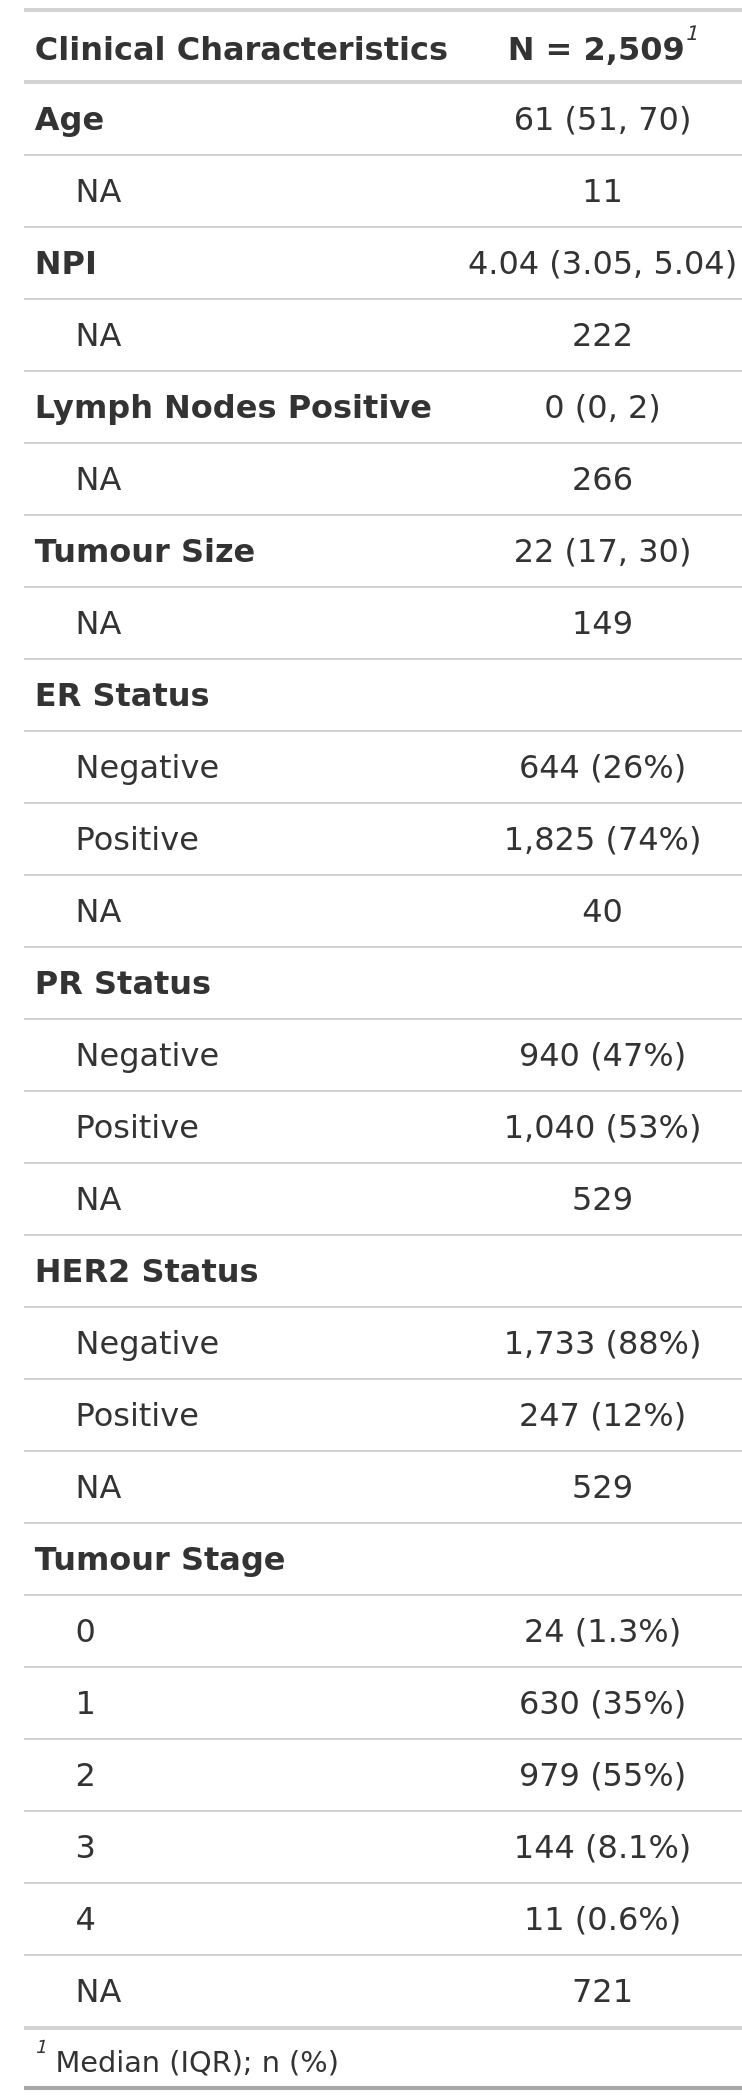
\includegraphics[height = 18cm]{../tables/Introduction/Table1_Clin_pt1.png}
\end{tabular}
\end{minipage}
\begin{minipage}[c]{0.5\textwidth}
\centering
\begin{tabular}{ccc}
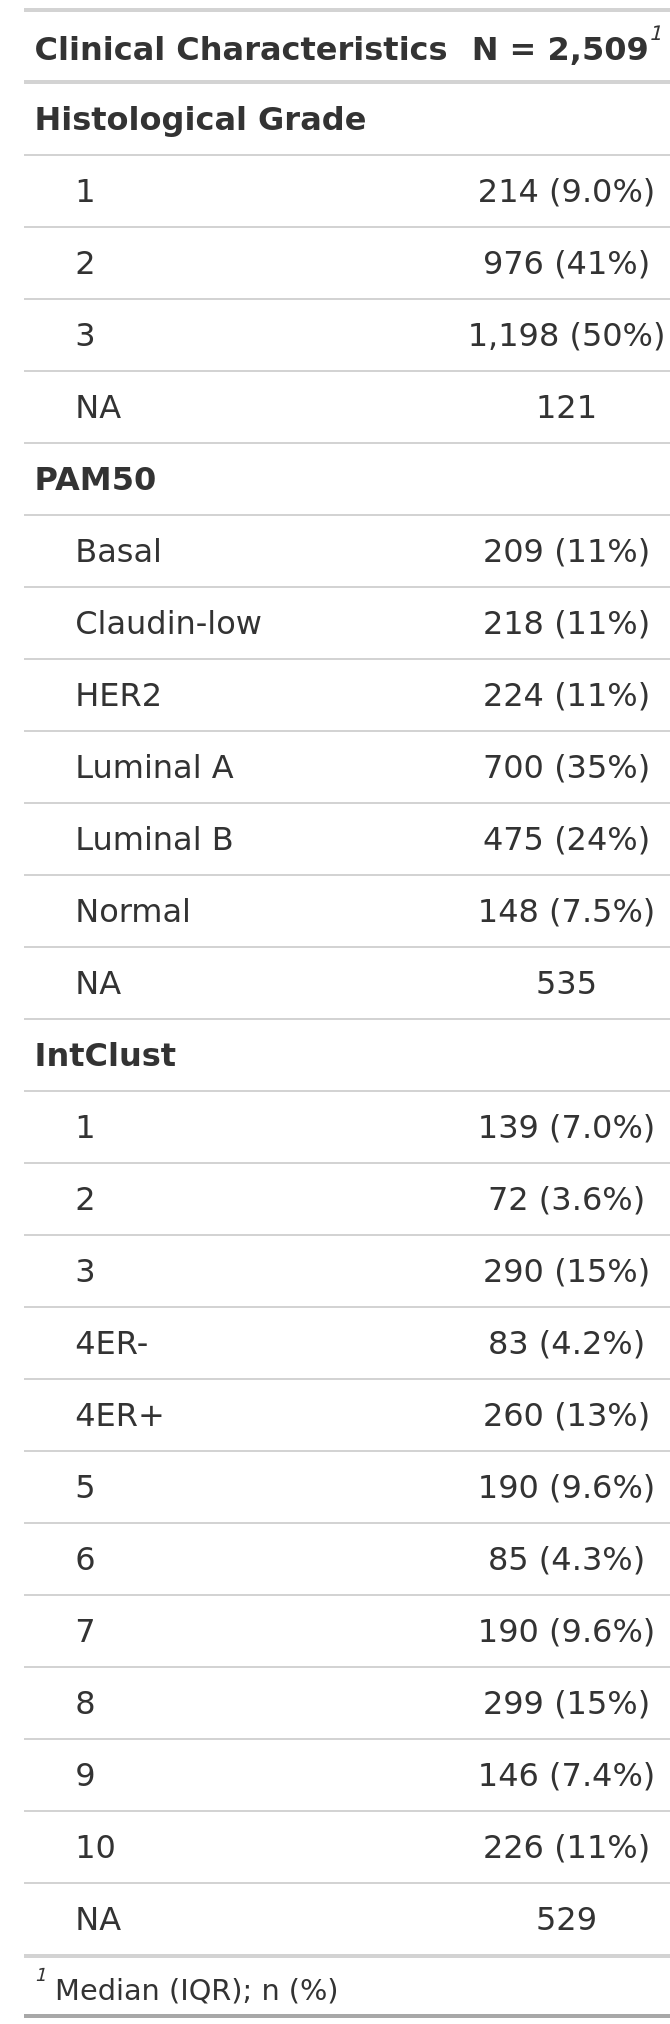
\includegraphics[height = 18cm]{../tables/Introduction/Table1_Clin_pt2.png}
\end{tabular}
\end{minipage}
\label{Clinchar}
\end{table}
\vfill 
\clearpage

\begin{figure}[H]
\center
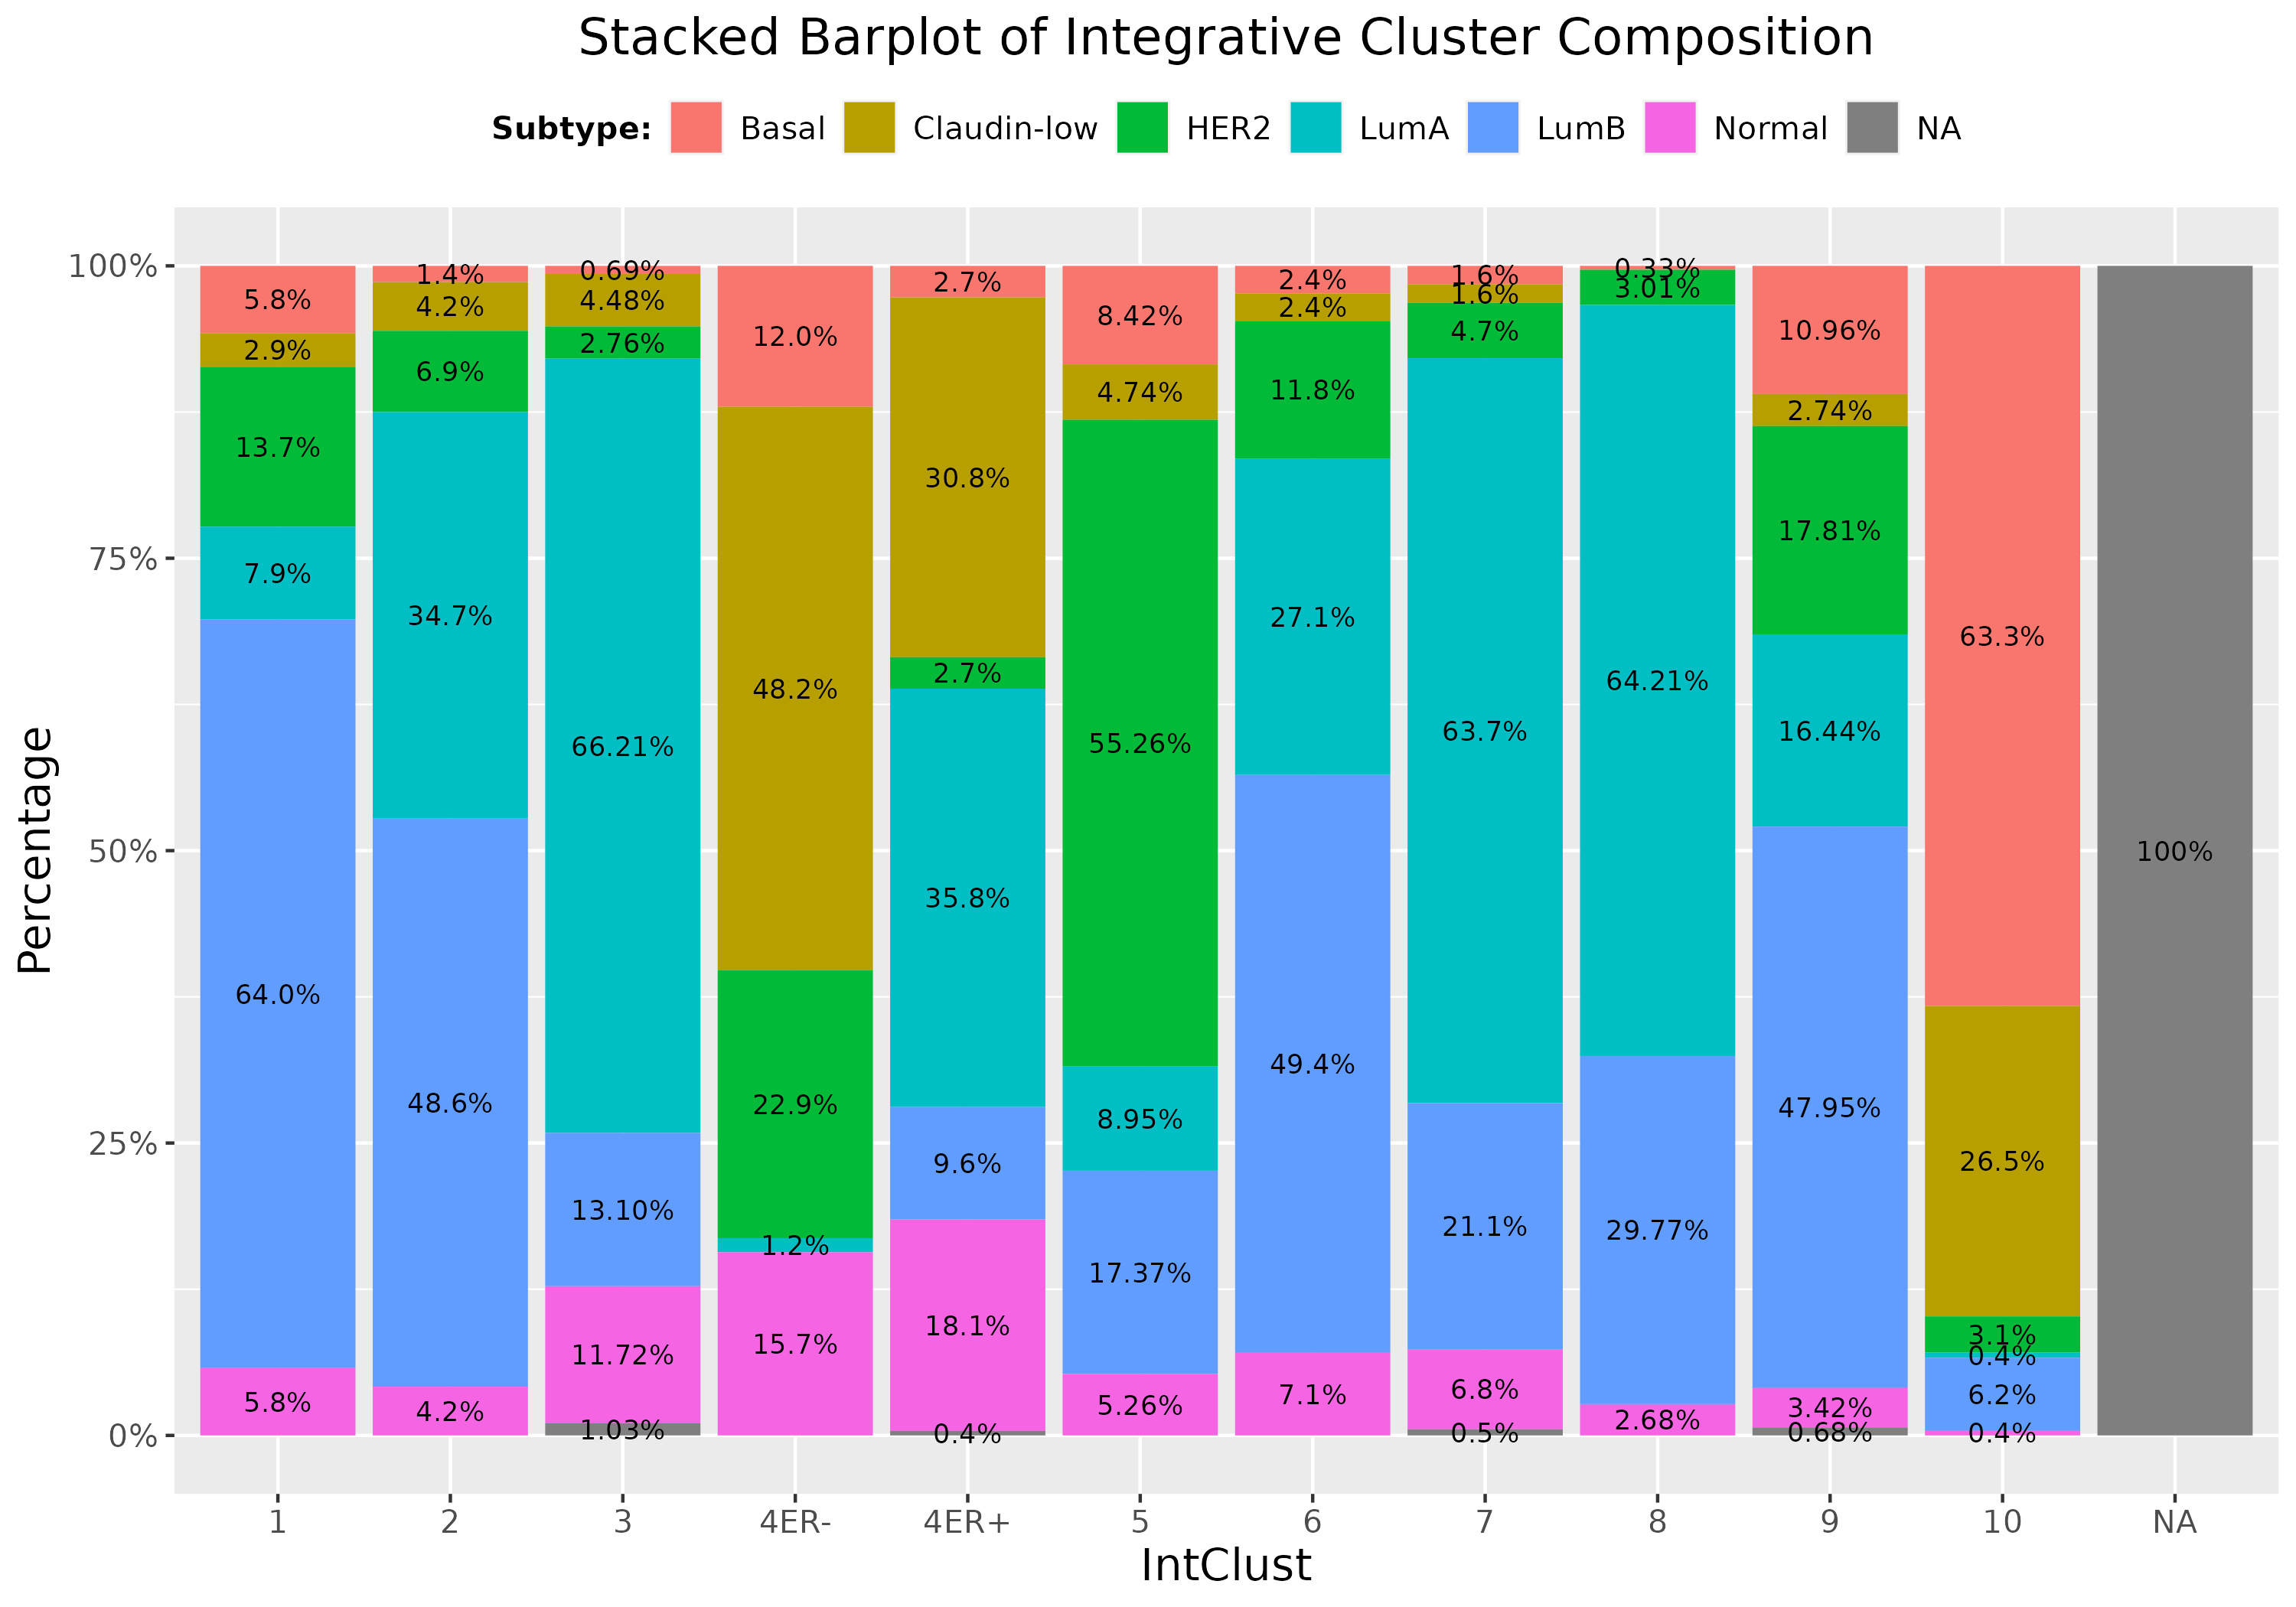
\includegraphics[width=0.94\textwidth]{../figures/Introduction/IntClust_Composition.png}
\caption[Stacked barplot indicating the PAM50 composition of each Integrative Cluster.]{Stacked barplot indicating the PAM50 composition of each Integrative Cluster. The x-axis denotes the Integrative Clusters and the y-axis percentages.}
\label{fig:Comp}
\end{figure} 

\begin{table}[H]
%\hspace{-1cm}
\begin{minipage}[c]{0.48\textwidth}
\centering
\caption{Treatment characteristics of the METABRIC patients.}
\begin{tabular}{ccc}
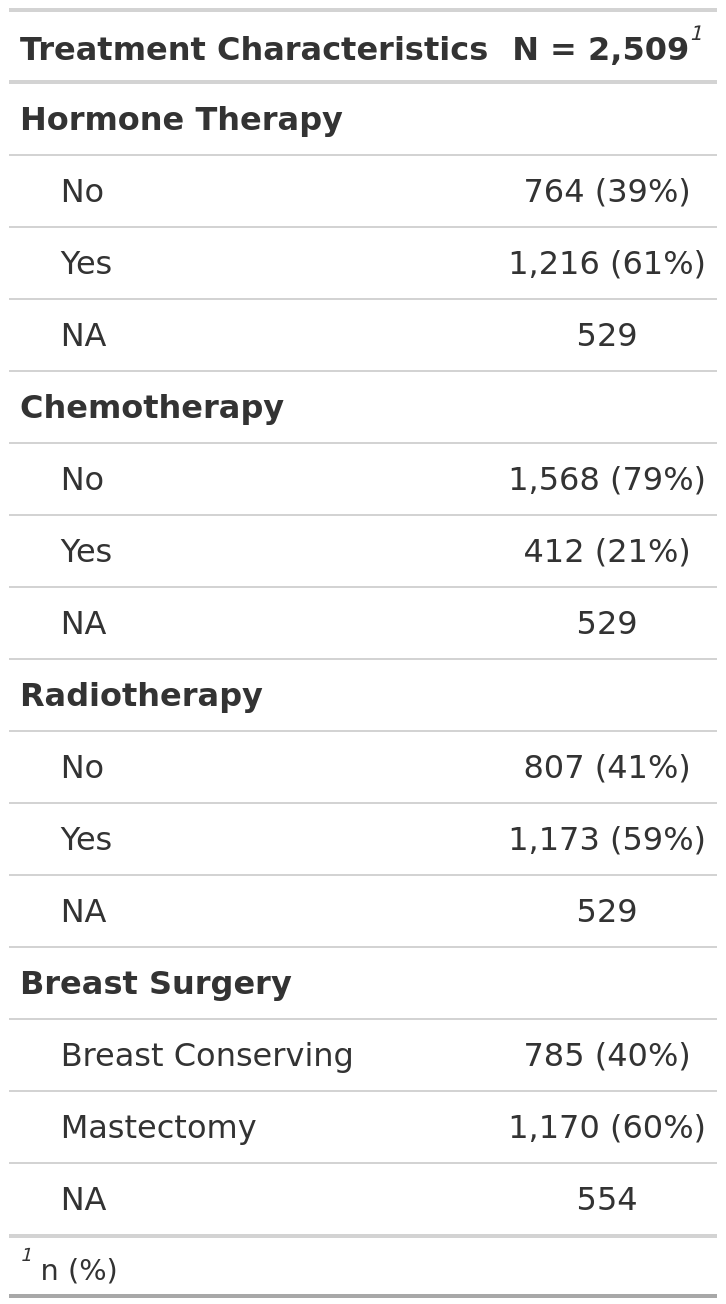
\includegraphics[height = 10.8cm]{../tables/Introduction/Table2_Treatment.png}
\label{Treatment}
\end{tabular}
\end{minipage}
\hspace{0.4cm}
\begin{minipage}[c]{0.48\textwidth}
\centering
\caption{Survival characteristics of the METABRIC patients.}
\begin{tabular}{ccc}
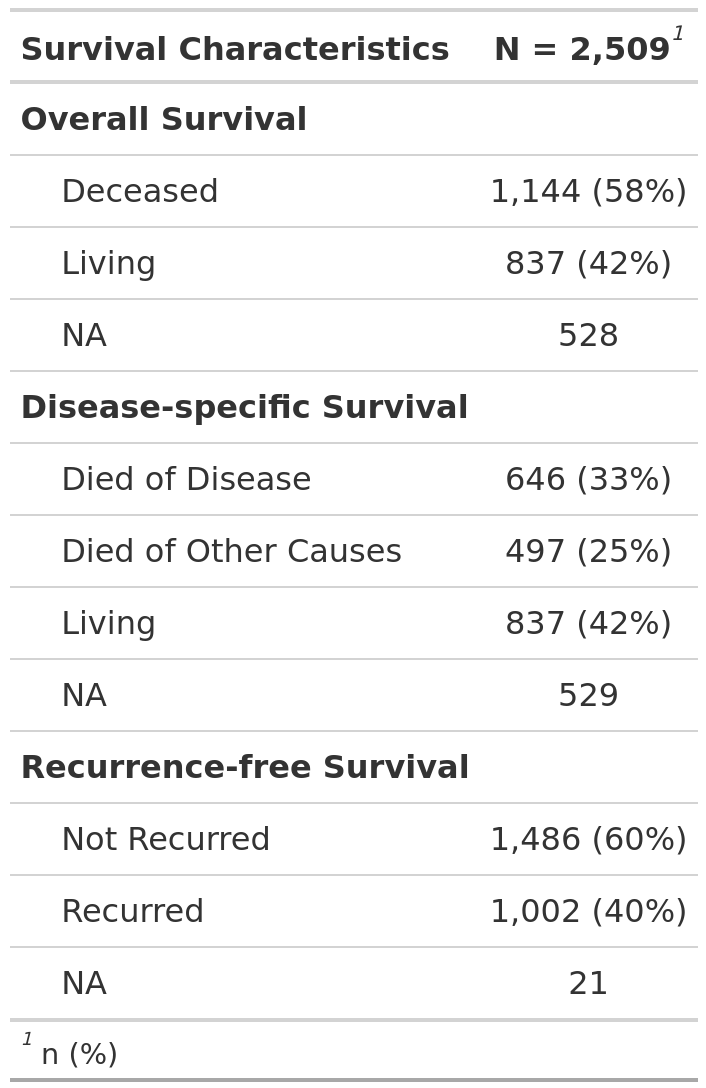
\includegraphics[height = 10.8cm]{../tables/Introduction/Table3_Survival.png}
\label{SurvTable}
\end{tabular}
\end{minipage}
\end{table}
 
These publicly available data are highly curated and periodically updated with additional information or datasets. Throughout this thesis the processed METABRIC data downloaded from cBioPortal are used “as is” and with the training and test sets defined in \cite{pmid22522925}, combined. Unless otherwise stated the results discussed in this thesis are based on the processed METABRIC data downloaded from cBioPortal in 2021.   

To obtain allele-specific CNA profiles, 1,992 Affymetrix SNP 6.0 CEL files available for 1,992 patients in the METABRIC study were accessed from the European Genome Phenome archive (study accession EGAS00000000083) \citep{pmid22522925, pmid34791407}. 

\subsection{Structure of Thesis}
Chapter 2 discusses CNAs as a measure of GI, with an introduction to published approaches for quantifying GI, and GI patterns in breast cancer. With application to the METABRIC cohort, novel CNA metrics are proposed, to measure individual patient CNA burden, accounting for the type, magnitude and location of the CNA. The distributions of the CNA metrics observed for the cohort are summarised, with an assessment of any effect from missing values. Distributions of CNA metrics are produced and summarised given location, e.g. global, or chromosome-arm specific, and are analysed comparing patients grouped by pre-defined breast cancer molecular classifications, such as PAM50 and IntClust.  

Chapter 3 investigates whether there is an association between the CNA metrics and survival outcomes, within the METABRIC cohort. A number of parametric, semi-parametric and non-parametric survival models are applied. Applications of survival trees demonstrate splits of patients into classification nodes using the molecular classifications and clinicopathological variables, while introducing the proposed CNA metrics as candidate predictors. 

Chapter 4 examines the effect of CNAs on gene expression, initially describing differential gene expression using limma and several expression-based predictive and prognostic assays for breast cancer. Differential gene expression analysis is carried out comparing gene expression between stratified groups of patients shown to have different survival outcomes, informed by models incorporating the CNA metric information. To finish, a comparative study is conducted, to compare the listing of differently expressed genes arrived at in this thesis, having incorporated CNA metric information, to the listings of prognostic and predictive gene sets previously derived and in use.

Chapter 5 focuses on allele-specific CNA profiles, CNA changepoints, and their identification and classification. The chapter reviews allele-specific copy number profiling using Allele-Specific Copy number Analysis of Tumours (ASCAT). Extraction of allele-specific CNA profiles using the PennCNV and ASCAT software is discussed and applied to the METABRIC cohort. Approaches to identify and model features of changepoints in allele-specific CNA profiles are proposed and include an extensive simulation study. 

Chapter 6 details application of allele-specific models to the METABRIC data. The models are applied to defined intervals, corresponding to gene regions and whole genome segments, and the genes and segments identified as containing CNA changepoints of significant length examined in the context of survival.  
\section{Copy Number Alterations as a Measure of Genomic Instability}
GI can be defined as an increased tendency for genomic alterations to occur. Genomic alterations, also termed genomic aberrations, include base substitutions, small insertions or deletions (indels), rearrangements, CNAs and even gain or loss of entire chromosomes and/or whole genome duplication \citep{pmid30736983, pmid31078431}. Two of the most well-characterised forms of GI are chromosomal instability (CIN) and microsatellite instability (MSI). CIN refers to changes in either chromosome number (numerical CIN), and/or structure (structural CIN), while MSI refers to the accumulation of mutations, usually point mutations or small indels, in microsatellite regions, i.e. regions of the genome displaying nucleotide repeats of about 1-6 bases in length \citep{pmid30736983, pmid31956294}.  

GI can occur as the result of defects in mechanisms including DNA replication, DNA damage repair, transcription, mitotic chromosome segregation, and telomere maintenance \citep{pmid26907526, pmid30736983, pmid31078431}. GI is a common feature of cancers and is recognised as a “facilitating” hallmark of cancer, enabling the activation of the eight functional hallmarks needed for tumour growth and progression \citep{pmid35022204}. While the degree of GI is variable within and between cancer types, the GI profile of a tumour can be thought of as the accumulation of genomic alterations, which have the potential to promote oncogenesis, affect progression and influence patient prognosis \citep{pmid26907526, pmid30736983}. In addition, the GI profile of a tumour can reflect the tumour's evolutionary history and future evolutionary potential \citep{pmid32242091}.

In this chapter, patterns of GI in breast cancer and several measures of GI utilised in the literature are discussed, a number of metrics based on CNAs are proposed, the effect of missing values on the CNA metric distributions assessed, and the distributions of these CNA metrics within pre-defined breast cancer molecular classifications (PAM50 and IntClust) analysed.

\subsection{Genomic Instability in Breast Cancer}
Breast cancer genomes are often tetraploid (4n) or near-triploid (3n), commonly have distinct gene expression patterns and often display specific numerical and complex structural chromosomal aberrations \citep{pmid31078431}. The exercise of classifying tumour samples or patients into groups of homogeneous gene expression patterns or CNA profiles identifies distinct genomic alteration patterns in breast cancer and provides a number of breast cancer classifications \citep{pmid28733194}. Here we focus on patterns and classifications based on CNA landscape.  

\cite{pmid17142309} described four distinct patterns of genomic alterations in breast cancer, termed “flat”, “simplex”, “complex I” and “complex II” (Figure \ref{fig:fig.hicks}). These patterns were identified using high-resolution comparative genome hybridisation arrays on 243 tumours selected from two breast cancer cohorts (140 samples were from the Cancer Center of the Karolinska Institute, while 103 were from the Oslo Micrometastasis study).

\begin{figure}[!htt]
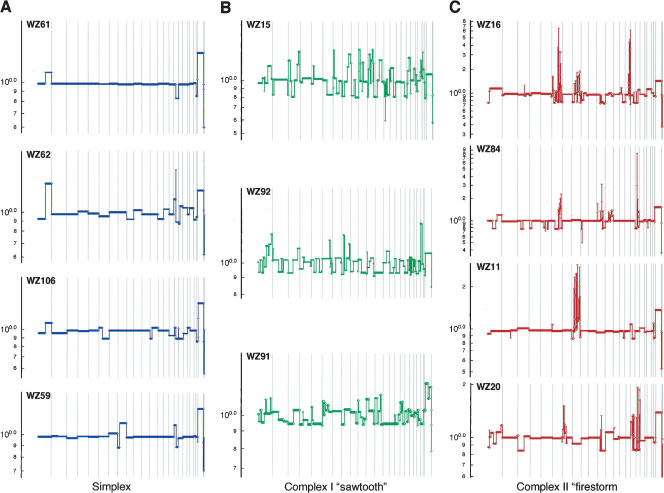
\includegraphics[width = 1\textwidth]{../figures/Chapter_2/Hicks_2006.jpg}
\caption[Distinct patterns of genomic rearrangements in breast cancer, taken from \cite{pmid17142309}.]{Distinct patterns of genomic rearrangements in breast cancer, taken from \cite{pmid17142309}. Segmentation profiles for individual tumours representing each category: (A) “Simplex” pattern (B) “Complex I”/“sawtooth” pattern (C) “Complex II”/“firestorm” pattern. The x-axis denotes chromosomes 1-22, X and Y, ordered from left to right, and the y-axis displays the geometric mean value of two experiments on a log scale.}
\label{fig:fig.hicks}
\end{figure}

Tumours displaying the “simplex” pattern have large segments of duplication and deletion that usually span entire chromosome arms or even chromosomes (Figure \ref{fig:fig.hicks}A). Frequent copy number changes observed within tumours displaying the “simplex” pattern include gain of chromosomes 1q, 8q and/or 16p and loss of chromosomes 16q, 8p and/or 22. These tumours are usually ER+ and of the Luminal subtype. Tumours displaying the “complex I” pattern, also termed the “sawtooth” pattern, have complex patterns of narrow, low-amplitude gains and losses. These gains and losses usually span short chromosome regions and are often alternating, resulting in regions with many copy number transitions (Figure \ref{fig:fig.hicks}B). These events commonly affect all chromosomes and lead to the majority of the genome undergoing copy number changes. Recurring copy number changes observed within tumours displaying the “complex I” pattern include regions of gain on chromosome 10p, and regions of loss on chromosomes 3p, 4p, 4q, 5q, 14q, 15q, and 17q. These tumours are usually triple-negative (ER-/PR-/HER-) and correspond to the Basal subtype. Tumours displaying the “complex II” pattern, also known as the “firestorm” pattern, resemble the “simplex” pattern except that the tumours contain at least one localised region of clustered narrow peaks of amplification, i.e. each amplification cluster is restricted to an individual chromosome or chromosome arm. These regions of amplification are referred to as amplicons and are usually separated by regions displaying normal copy number or deletions (Figure \ref{fig:fig.hicks}C). Recurrently amplified sites include FGFR1, MYC, CCND1, MDM2, ERBB2 (HER2), and ZNF217. These tumours are usually of the Luminal B and HER2 subtype. Tumours displaying the “flat” pattern have no clear amplifications or deletions except copy number polymorphisms \citep{pmid17142309, pmid28733194}. 

To relate these patterns to clinical outcome, \cite{pmid17142309} developed the Firestorm Index. Using this metric, it was observed that the “complex I” and “complex II” patterns were associated with more aggressive disease and worse survival outcomes. 

\cite{pmid27136393} provides a classification based on rearrangement signatures derived from 560 breast cancer whole genome sequences. Six rearrangement signatures (RS1-RS6) were created, based on whether the rearrangement was a deletion, tandem duplication, inversion, or translocation, the size of the rearrangement and also whether the rearrangements occurred in close proximity to each other. Interestingly, \cite{pmid28733194} noted that these signatures relate back to the classification described in \cite{pmid17142309}. RS1 and RS3 are characterised by tandem duplications similar to the “complex I” or “sawtooth” pattern, RS4 and RS6 by clustered rearrangements similar to the “complex II” or “firestorm” pattern, RS5 by deletions, and RS2 by translocations, similar to the “simplex” pattern. For most tumours, the genomic landscape of rearrangements is composed of combinations of these signatures \citep{pmid27136393, pmid28733194}.

\cite{pmid22522925} used gene expression data along with CNA data, of 1,992 breast cancer samples from the METABRIC cohort, to identify ten distinct subtypes of breast cancer. Initially, using Analysis of Variance (ANOVA) and the Kruskal-Wallis test, they identified genes where the presence of a CNA influenced the expression of that gene, i.e. where overexpression is associated with copy number gain or amplification and underexpression with copy number loss. This method, by definition, captures genomic drivers, oncogenes and tumour suppressor genes whose expression is associated with copy number changes. The 1,000 most significant cis-driven genes, in terms of Bonferroni corrected p-values, were inputted as explanatory variables in a joint latent variable framework for integrative clustering. The most parsimonious solution, with reference to copy number profiles, risk patterns, and prognosis, classified tumours into ten distinct groups (IntClust 1-10, Figure \ref{fig:fig.IC}). %Table \ref{tbl:IC}, produced by \cite{pmid23395906}, documents the features of the integrative clusters.

\begin{figure}[h]
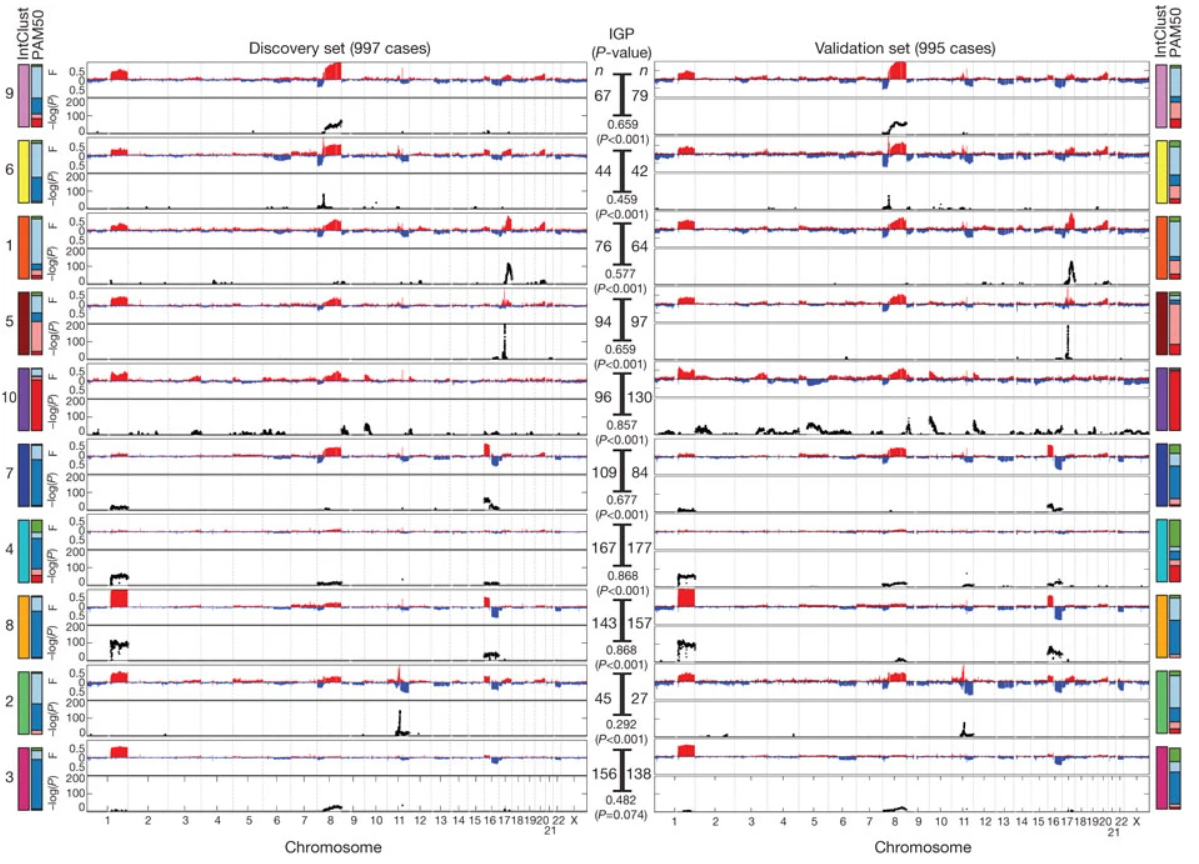
\includegraphics[width = 1\textwidth]{../figures/Chapter_2/IntClust_Profiles_Curtis.png}
\caption[Distinct copy number profiles of the Integrative Clusters, taken from \cite{pmid22522925}.]{Distinct copy number profiles of the Integrative Clusters, taken from \cite{pmid22522925}. Frequencies of CNAs are displayed on the upper y-axis of each section and the subtype-specific association (-log10 p-value) of aberrations is displayed on the bottom y-axis. Regions of copy number gain are indicated in red and regions of loss in blue. The distribution of PAM50 subtypes within each cluster is also shown.}
\label{fig:fig.IC}
\end{figure}

\subsection{Measures of Genomic Instability}
\label{MeasureGI} 
To explore the impact of GI in cancer, a number of genomic and transcriptomic signatures have been created to quantify levels of GI in tumours, and their prognostic and predictive power assessed. These metrics, summarised in Table \ref{tab:GI}, are described below.

% Please add the following required packages to your document preamble:
% \usepackage{graphicx}
\begin{table}[!htb]
\caption{Summary of existing measures of Genomic Instability.}
\resizebox{\textwidth}{!}{%
\begin{tabular}{|l|l|l|l|l|}
\hline
\textbf{GI Measure}                                                                                         & \textbf{Cancer Type(s)}                                                                                                                                                                   & \textbf{Input Data}  & \textbf{Platform(s) Used in Study}                                                                                                        & \textbf{Author}                                                                        \\ \hline
CIN25 and CIN75                                                                                             & \begin{tabular}[c]{@{}l@{}}Breast cancer, lung adenocarcinoma, \\ small-cell lung cancer, mesothelioma, \\ prostate cancer, B-cell lymphoma, \\ ovarian cancer, glioma, medulloblastoma\end{tabular} & Gene expression data & \begin{tabular}[c]{@{}l@{}}Affymetrix Human Genome \\ U133A microarray \\ Affymetrix Human Genome \\ U133+2 microarray \\ Rosetta 25k microarray\end{tabular} & \cite{pmid16921376} \\ \hline
Chromosomal Instability Score                                                                               & Breast cancer                                                                                                                                                                                        & Copy number data     & \begin{tabular}[c]{@{}l@{}}Affymetrix GeneChip Mapping \\ 100K microarray                                                                                           \end{tabular} & \cite{pmid20632083} \\ \hline
\begin{tabular}[c]{@{}l@{}} Centromere and Kinetochore \\ Gene Expression Score\end{tabular}
& \begin{tabular}[c]{@{}l@{}}Breast, lung, ovarian, liver, pancreatic, \\ colon, nasopharyngeal, gastric, cervical, \\ head and neck, prostate, brain.\end{tabular}                                     & Gene expression data & \begin{tabular}[c]{@{}l@{}}Affymetrix Human Genome \\ U133+2 microarray\end{tabular}                                                                                                         & \cite{pmid27577169}                                                                     \\ \hline
Chromosomal Instability Index                                                                               & Colorectal cancer                                                                                                                                                                                    & Copy number data     & \begin{tabular}[c]{@{}l@{}}Affymetrix Genome-wide Human \\ SNP array 6.0                                                                                            \end{tabular}  & \cite{pmid29343938} \\ \hline
\begin{tabular}[c]{@{}l@{}}Whole Arm Aberration Index and \\ Complex Arm‐Wise Aberration Index\end{tabular} & Breast cancer                                                                                                                                                                                        & Copy number data     & \begin{tabular}[c]{@{}l@{}}
Custom ROMA 85k microarray \\
Agilent Human Genome CGH \\ 244K microarray \\
Custom Human 30K 60-mer \\ oligo microarray
\end{tabular}                                                        & \cite{pmid20592421}                                                                   \\ \hline
Firestorm Index                                                                                             & Breast cancer                                                                                                                                                                                        & Copy number data & Custom ROMA 85k microarray & \cite{pmid17142309} \\ \hline
Copy Number Alteration Burden                                                                               & Prostate cancer, breast cancer                                                                                                                                                                       & Copy number data     & \begin{tabular}[c]{@{}l@{}}Agilent Human CGH Whole \\ Genome microarray \\ Affymetrix Genome-wide Human \\ SNP array 6.0 \end{tabular}                                                                                             & \begin{tabular}[c]{@{}l@{}}\cite{pmid25024180} \\ \cite{pmid30178746} \\ \cite{pmid30337938}\end{tabular} \\ \hline
\begin{tabular}[c]{@{}l@{}}Copy Aberration Regional Mapping \\ Analysis Scores \end{tabular}                                                            & Breast cancer                                                                                                                                                                                        & Copy number data     & \begin{tabular}[c]{@{}l@{}}Affymetrix Genome-wide Human \\ SNP array 6.0                                                                                            \end{tabular} & \cite{pmid32242091} \\ \hline
Genomic Instability Index                                                                                   & Breast cancer                                                                                                                                                                                        & Copy number data     & \begin{tabular}[c]{@{}l@{}}Custom Human 30K 60-mer \\ oligo microarray\end{tabular} & \cite{pmid17925008} \\ \hline
\begin{tabular}[c]{@{}l@{}}Genomic Identification of Significant \\ Targets in Cancer \end{tabular} & Glioma                                                                                                                                                                                               & Copy number data     & \begin{tabular}[c]{@{}l@{}}Affymetrix Human Mapping 50K \\ Xba240 SNP array\\ Affymetrix Human Mapping 50k \\ Hind240 SNP array\end{tabular} & \cite{pmid18077431}                                                                  \\ \hline
\end{tabular}%
}
\label{tab:GI}
\end{table}

\subsubsection{Expression Based Signature CIN25 and CIN70}
It has been well documented that correspondence exists between gene expression changes and CNAs in regions relevant to those genes \citep{pmid12297621, pmid17289997,  pmid22522925, pmid32024838}. \cite{pmid16921376} derived two expression-based signatures, reflecting CIN in tumours, termed CIN25 and CIN70, using 25 and 70 genes, respectively. These signatures were developed using integrated gene expression data from 18 studies, across nine cancer types, totalling 1,944 samples. These signatures are based on a functional aneuploidy measure (FA) calculated across cytobands, i.e. genomic regions corresponding to the approximate location of bands seen on Giemsa-stained chromosomes. For a given dataset, a cytoband specific \textit{t}-statistic compares normalised gene expression measurements mapped to a specific cytoband, group B, to the normalised gene expression measurements for the genes mapped to all other cytobands, group G: 

\begin{equation}
t = \frac{\mu_B - \mu_G}{\sqrt{(\frac{\sigma^2_B}{N_B}) + \frac{\sigma^2_G}{N_G})}}
\end{equation}

where $\mu_B$, $\mu_G$ are the observed means, $\sigma^2_B$,  $\sigma^2_G$, are the observed variances, and $N_B$, $N_G$, the number of genes, for groups B and G.

The total FA (tFA) for each sample, within each of the 18 datasets, was defined as the sum of all FA magnitudes (the absolute \textit{t} statistics), across each cytoband with more than 10 genes recorded, in that sample. For all genes within each dataset, the correlation coefficient across all samples between each gene's expression vector (the vector containing that genes expression for all samples in that dataset) and the tFA vector (the vector containing the tFA for each sample in that dataset) was computed. Genes in each dataset were then ranked based on the value of the correlation coefficient. Following normalisation of ranks within each dataset, the total of the ranks of a gene within three selected datasets was used as the final integrated ranking for the gene. The top 25 and 70 genes from this ranking formed the CIN25 and CIN70 signature, respectively.

tFA was found to be significantly correlated with aneuploidy assessed using CNA profiles and structural chromosomal aberrations from spectral karyotyping on NCI-60 cell lines. Furthermore, the CIN25 and CIN70 genes showed significant deviation in their expression relative to the remainder of the transcriptome and were enriched for regulators of mitotic spindle assembly, the mitotic checkpoint, and the DNA damage checkpoint.

To explore the prognostic power of CIN25 and CIN70, patients were split into two groups, patients with total expression, i.e. sum of the log-ratio measures, above the mean signature expression, and patients below the mean signature expression, in all samples from that dataset. This indicated that the CIN25 signature was a significant predictor of clinical outcome in 12 out of 18 cancer datasets and the CIN70 signature was a significant predictor of clinical outcome in 13 out of 18 datasets. Comparing the CIN25 and CIN70 signatures between primary and metastatic tumours also indicated metastatic samples display higher levels of the CIN signatures compared to primary tumours.

\subsubsection{Chromosomal Instability Score}
\cite{pmid20632083} used SNP copy number data from 313 primary lymph-node negative breast cancers to study the prognostic relevance of CIN within breast cancer subtypes. In this study, by measuring the loss, gain, or diploid status of SNPs within 100-kilobase (kb) genomic windows, a measure for CIN was defined as the total number of chromosomal segments showing a gain or loss. Hierarchical clustering of patients using this CIN metric identified four main groups showing varying degrees of chromosomal abnormalities. In addition, it was found that high CIN score was significantly associated with worse prognosis in ER+, Luminal B, and HER2 subtypes, but not in ER- patients. 

\subsubsection{Centromere and Kinetochore Gene Expression Score}
Centromeres and kinetochores play essential roles in cell division and their protein level is usually tightly regulated \citep{pmid19002142}. Their dysfunction can result in a number of misregulation effects, including missegregation and mislocalisation to non-centromeric chromatin, generating neo-centromeres, dicentric behaviour and chromosome bridges, that drive aneuploidy and CIN (gains and losses) \citep{pmid19002142, pmid27577169}. To capture this misregulation, \cite{pmid27577169} developed the centromere and kinetochore gene expression score (CES) that quantifies the misexpression of 14 centromere and kinetochore genes in cancers. To arrive at this scoring mechanism, expression profiles of 31 candidate centromere and kinetochore genes were analysed, 15 of these genes were observed to be significantly misregulated and of these, 14 were found to be associated with poor patient survival and correlated with cancer progression, in an analysis of 18 different cancer datasets from The Cancer Genome Atlas (TCGA). CES is calculated as the sum of the log$_2$ mRNA expression level of the 14 centromere and kinetochore genes. It was shown that high CES significantly correlated with increased CIN and accurately predicts patient outcome in terms of OS, distant metastasis-free survival and relapse-free survival. This study also reported that high CES cell lines were sensitive to genotoxic drugs, such as campthothecin, topotecan and irinotecan.

\subsubsection{Chromosomal Instability Index}
The CIN index is a measurement that quantitatively characterises genome-wide CNAs. The CINdex algorithm uses segmented copy number data to calculate global measures of GI across chromosomes and at a higher resolution across cytobands. The first step in calculating CIN index involves calling segments as either gain or loss. A segment with mean signal intensity greater than an assigned threshold, $t_{gain}$, is called as a gain, whereas a segment with mean signal intensity smaller than an assigned threshold, $t_{loss}$, is called as a loss. In \cite{pmid29343938} the biologically experimental values of $t_{gain}$ and $t_{loss}$ are 2.5 and 1.5, respectively. Subsequently, the amplitude of change is scaled to make maximal losses and maximal gains comparable in magnitude. To do this, the amplitude of each loss segment, $a$, is converted to the new value, $a'$, based on the relationship given by: 

\begin{equation}
(t_{loss} - a)/a = (a'-t_{gain})/(A - t_{gain})
\end{equation}

where $A$ is maximum gain amplitude across all samples and segments and $t_{loss}$ and $t_{gain}$ are the assigned thresholds for calling losses and gains, respectively. 

The chromosome-specific instability index for each sample is calculated using:

\begin{equation}
CIN_i = (\sum_ka_k + \sum_ja'_j)/N
\end{equation}

where \textit{N} is the number of SNP probes on chromosome $i$, $a$ is the amplitude of gain segments and $a’$ is the amplitude of loss segments. 

Applying the same calculation at the cytoband level provides the cytoband-specific instability index. The CINdex Bioconductor package \citep{CINdex} implements this algorithm and generates a chromosome and cytoband CIN value for each sample. The package also enables comparison of CIN index values between groups of patients to identify differentially altered chromosomes or cytobands. Genes within these differentially altered regions can then be identified and pathway enrichment performed. 

\subsubsection{Whole Arm Aberration Index and Complex Arm‐Wise Aberration Index}
\cite{pmid20592421} developed two algorithms to characterise levels of genomic distortion using array comparative genomic hybridisation (aCGH) data. These algorithms are termed the Whole Arm Aberration Index (WAAI) and the Complex Arm Aberration Index (CAAI), where WAAI aims to capture whole-arm deviations from normal copy number, i.e. whole-arm gains/losses, and CAAI aims to capture the degree of local distortion i.e complex rearrangements. 

WAAI is calculated across each chromosome arm for each sample. The first step in generating the WAAI values is to use the Piecewise Constant Fitting (PCF) algorithm to fit a piecewise constant regression function to the log-transformed aCGH data for each sample. As a result, a fitted value, termed “PCF-value”, is obtained for each probe. The centred PCF-values were then divided by the residual standard deviation to produce normalised PCF (NPCF)-values and a new variable $s$ was obtained by averaging the NPCF-values over all probes. If $s > 0$, WAAI was the 5\% quantile of NPCF and if $s \leq 0$, WAAI was the 95\% quantile of NPCF. Chromosome arms with WAAI $\ge 0.8$ were called as whole-arm gains, and chromosome arms with WAAI $\leq -0.8$ were called as whole arm losses. 

CAAI is also calculated across each chromosome arm for each sample. In the original paper a threshold of 0.5 was applied to create a two-category CAAI variable, whereas it is possible to use the CAAI as a continuous variable \citep{pmid32242091}. The first step in generating the CAAI variable is to use the PCF algorithm to fit a piecewise constant regression function to the log-transformed aCGH data for each sample. Then for each breakpoint (chromosomal position affected by rearrangements) identified by PCF, three scores, P, Q and W, were calculated. To produce the CAAI variable from the original paper, P, Q and W are defined as follows: 

\begin{equation}
P = tanh \left( \frac{\alpha}{L1 + L2} \right)
\end{equation}
\begin{equation}
Q = tanh(|H2 - H1|)
\end{equation}
\begin{equation}
W = 0.5 \left[1 + \frac{tanh(10(P-0.5))}{tanh(5)} \right]
\end{equation}

where $\alpha$ is a constant. For any given breakpoint, $L1$ and $L2$ denote the number of nucleotides in each segment and $H1$ and $H2$ denote their scaled PCF-values.  

\cite{pmid32242091}, proposed a refined version of the CAAI variable, where P, Q and W are defined as: 

\begin{equation}
P = tanh \left(\frac{\alpha}{L1 + L2} \right)
\end{equation}
\begin{equation}
Q = tanh(\beta \cdot |H1 - H2|)
\end{equation}
\begin{equation}
W = 0.5 \left[1 + \frac{tanh(10P - 5)}{tanh(5)} \right]
\end{equation}

where $\alpha$ and $\beta$ are constants $2 \cdot 10^6$ and $\frac{1}{1.2}$, respectively. For any given breakpoint, $L1$ and $L2$ denote the size of the segments joined and $H1$ and $H2$ denote their height, i.e. total copy number. 

These three scores P, Q and W, reflect the proximity to neighbouring breakpoints, the magnitude of change and a weight of importance. Subsequently, CAAI is defined as the maximal value of $\sum W \cdot min(P, Q)$ across all breakpoints within a region of predefined size, i.e. 20 megabases (Mb).

Applying CAAI and WAAI to data from 595 breast cancer patients from four clinical cohorts (MicMa cohort, WZ cohort, Chin-UCAM cohort and Ull cohort), patients were split into eight subgroups each with distinct patterns of genomic alterations. CAAI was observed to be highly prognostic for DSS and OS in breast cancer. In addition, CAAI also correlates with expression-based prognostic signatures including MammaPrint and OncotypeDX. Subsequently, \cite{pmid25169931} validated CAAI as an independent prognostic indicator in breast cancer and also showed that CAAI could act as a prognostic indicator in high-grade serous ovarian cancer.

\subsubsection{Firestorm Index}
\label{MeasureGIFI}
\cite{pmid17142309} noted that the “complex I”/“sawtooth” and “complex II”/“firestorm” patterns often correlated with aggressive disease and worse survival in diploid tumours. To confirm this, the authors created a metric which separates the highly rearranged “complex I”/“sawtooth” and “complex II”/“firestorm” from the “flat” and “simplex” patterns. To distinguish the “complex II”/“firestorm” pattern from the “simplex” pattern this metric considered both the tightly packed spacing of the firestorm events and the total number of events. This metric, termed the Firestorm index (F), is obtained by summation across the reciprocals of the mean of lengths of all adjacent segment pairs: 

\begin{equation}
F = \sum_i{\frac{2}{l_i^L + l_i^R}}
\end{equation}

where $i$ corresponds to the set of all discontinuities or breaks with a magnitude above the threshold of 0.1, $l_i^L$ and $l_i^R$ correspond to the number of probes in the nearest discontinuity to the left or right, respectively, or to a chromosome boundary, whichever is closer.

This metric can distinguish the “complex II”/“firestorm” pattern from the “simplex” pattern and assigns high F values to the complex patterns. The “complex I”/“sawtooth” pattern will have a high F value as a result of the high number of events across a large number of chromosomes, while the “complex II”/“firestorm” pattern will have a high F value due to the sparse events occurring in close proximity. \cite{pmid17142309} also reported a strong association between F and survival outcomes.

\subsubsection{Copy Number Alteration Burden}
\label{CNABurden}
CNA Burden is defined as a measure of the percentage of the genome affected by CNAs, calculated as the summation of the lengths of all CNA (gain and loss) segments as a percentage of the total length of the autosomal genome. 

A number of studies have reported an association between CNA burden and recurrence, metastasis, OS and DSS \citep{pmid25024180, pmid30178746, pmid30337938}. \cite{pmid25024180} showed that CNA burden is prognostic for prostate cancer recurrence and metastasis, \cite{pmid30178746} observed that CNA burden is associated with both OS and DSS in a range of cancers including breast, endometrial, renal, thyroid, and colorectal cancer and \cite{pmid30337938} showed that there is a significant association between CNA burden and OS and DSS in breast cancer cohorts.

\subsubsection{Copy Aberration Regional Mapping Analysis Scores}
\label{CARMA}
\cite{pmid32242091} developed the Copy Aberration Regional Mapping Analysis (CARMA) algorithm which identifies multiple local copy number features, or “motifs”, across a pre-defined region and combines these to create regional metrics. CARMA takes allele-specific copy number profiles as inputs and produces six metrics that aim to capture the degree of amplification (AMP), deletion (DEL), complexity, i.e. chromothripsis and chromoplexy (STP and CRV), loss of heterozygosity (LOH) and allelic imbalance or asymmetry (ASM). Together, these metrics consider copy number magnitude, the spatial distribution of copy number breakpoints, allelic imbalance and regional fluctuations in copy number.  

These scores are defined using continuous functions on genomic loci, i.e. positions on a chromosome, $t_1, …, t_i$, over a region R. Here, $f(t)$ is the median centred total copy number in locus $t$ and is calculated by $f(t) = f_A(t) + f_B(t) - m$, where $f_A(t)$ and $f_B(t)$ are piecewise constant functions representing the allele-specific copy number profiles of the major allele and minor allele, respectively, and $m$ is chosen as the median observed copy number.   

The degree of amplification AMP is defined as:

\begin{equation}
AMP = \int_{R}{\{f(t)_+\}^2} 
\end{equation}

where $f(t)_+$ corresponds to the regions where the median centred total copy number is greater than 0. Alternatively, one can think of this metric as $AMP = \sum L_+ \times H_+^2$, where $L_+$ is a vector containing the scaled lengths of segments where an amplification is present, relative to the median copy number, and $H_+$ is a vector containing the corresponding copy number magnitudes. AMP will take value 0 where the total copy number is equal to the median copy number and greater than 0 when there are some gains and no losses relative to the median. 

Similarly, the degree of deletion is defined as: 

\begin{equation}
DEL = \int_{R}{\{f(t)_-\}^2}
\end{equation}

where $f(t)_-$ corresponds to the regions where the median centred total copy number is less than 0. DEL will take value 0 where the total copy number is equal to the median and greater than 0, where there are some losses and no gains relative to the median.   

The complexity scores are defined as: 

\begin{equation}
STP = \int_{R}{\{Df(t)\}^2} dt
\end{equation}
\begin{equation}
CRV = \int_{R}{\{D^2f(t)\}^2} dt
\end{equation} 

where $Df(t)$ is the first derivative and $D^2f(t)$ is the second derivative, reflecting the change in total copy number and the oscillation in total copy number, respectively. STP will take value 0 where there is constant total copy number and greater than 0 where there is gradually increasing or decreasing copy number, or where there are fluctuations between smaller and larger copy numbers. CRV will take value 0 where the copy number is constant, be close to 0 where there is gradually increasing or decreasing copy number and greater than 0 where there are fluctuations between smaller and larger copy numbers. 

Loss of heterozygosity is defined as: 

\begin{equation}
LOH =  \int_{R}{\{1_0(f_B(t))\}} dt
\end{equation}

where $f_B(t)$ is the piecewise constant function representing the copy number profile of the minor allele, $1_0$ is an indicator variable informing whether or not the minor allele is lost. If the copy number of the minor allele is 0 at locus $t$ then $1_0 = 1$, otherwise $1_0 =0$. Alternatively, one can think of this metric as $LOH = \sum L[minor = 0]$, where $L$ is a vector containing the scaled lengths of segments where the minor allele has been lost, i.e. copy number is 0. LOH takes a value greater than 0 where the minor allele has been lost, with the magnitude of the metric reflecting the proportion of the region with LOH. 

Allelic imbalance or asymmetry is defined as:  

\begin{equation}
ASM = \int_{R}{\{(f_A(t) - f_B(t))^2\}} dt
\end{equation}

where $f_A(t)$ and $f_B(t)$ are the piecewise constant functions representing the copy number profile of the major allele and the minor allele, respectively, so that ASM $> 0$ in regions of allelic imbalance. 

The authors applied CARMA to four breast cancer cohorts, METABRIC (n = 1,943), Oslo2 (n = 276), OsloVal (n = 165), and ICGC (n = 553). To standardise the scores, all six scores were log$_2$-transformed and normalised by dividing by the 99th percentile in the METABRIC discovery set. The authors showed that the CARMA metrics correlated with the CAAI and CINdex metrics and provided significantly more detail about the copy number profile, enabling identification of alterations that may not be captured by the other methods. For example, in a region where there is loss of one allele and gain of the other, the CINdex would indicate that no alteration has occurred, whereas the LOH and ASM metrics would capture this event. The authors also considered the distribution of CARMA scores within breast cancer subtype classifications (PAM50 and IntClust) and noted that the CARMA scores captured differences in the genomic landscapes of the distinct subtypes. 

Examining whether the CARMA metrics were significantly associated with survival outcome, univariate Cox proportional hazards regression models were fitted for each metric, and these models indicated that all CARMA metrics were associated with DSS. To assess if the presence or absence of the copy number motifs was significantly associated with survival outcome, the information provided by all six CARMA metrics was combined into two prognostic indices, the CARMA Prognostic Index (CPI) and the weighted CPI ($\text{CPI}_\text{weighted}$). Briefly, using a discovery set and test set from the observed cohort, the CPI index was produced by fitting multivariate Cox regression models for DSS outcome and progression-free survival outcome, using the unweighted mean of the six CARMA metrics as predictors. The fitted model was then applied to the test set, producing a single unweighted prognostic value for each patient in the test set. 

Patients were stratified into low, intermediate, and high-risk groups, of equal cohort size, based on their CPI value. These tertile groups are defined as having CPI score, 1, 2, and 3, respectively. The $\text{CPI}_\text{weighted}$ score was produced using the 252 arm-wise CARMA scores directly as predictors and fitting a Cox regression model with LASSO penalty to the discovery set. Coefficients derived from the model were then used as weights to calculate the $\text{CPI}_\text{weighted}$. Both CPI and $\text{CPI}_\text{weighted}$ were shown to be significantly associated with DSS and progression-free survival before and after adjusting for other relevant clinical variables. Patients in the high-risk CPI group displayed significantly worse DSS and progression-free survival.

\subsubsection{Genomic Instability Index}
The Genomic Instability Index (GII) is defined as the fraction of the genome with CNAs. \cite{pmid17925008} proposed two GII metrics, calculated based on the fraction of the genome that was altered using common regions of alteration (CRA), regions that were altered in at least 5\% of tumours, and on the fraction of altered probes. As expected, a very strong correlation was observed between the two GII metrics (Spearman rank correlation 0.96). Using hierarchical clustering, on the CRA from 171 primary breast tumours, the authors identified a novel subtype of high-grade ER- breast cancer, characterised by a low GII. With this index the authors documented regions across the breast cancer genome that frequently contain CNAs and have corresponding dysregulated expression. Furthermore, they identified regions of the genome that were frequently amplified and correlated with poor prognosis, with some of these regions not previously identified. 

\subsubsection{Genomic Identification of Significant Targets in Cancer} 
\cite{pmid18077431} introduced the Genomic Identification of Significant Targets in Cancer (GISTIC) algorithm which differs from the previously mentioned GI measures/algorithms in that it identifies regions within the genome that are significantly altered across multiple samples. GISTIC produces multiple outputs, including a categorical value (0, 1 or 2) of aberration for each region and each sample. The GISTIC algorithm first assigns a score (G score) to each aberration, which reflects the aberration amplitude and the frequency with which the aberration occurs across samples, the significance of each aberration is assessed using permutation tests based on the overall pattern of aberrations observed across the genome. Regions with false discovery rates below a given threshold are declared to be significant aberration regions. For each significant aberration region, GISTIC defines a “peak region”, containing the highest frequency and amplitude of aberration, and determines whether the signal is due to broad events, focal events, or both.    
GISTIC has been applied to multiple cancer types and has identified a number of new targets of deletions and amplifications such as EHMT1 in medulloblastoma and CDK8 in colorectal carcinoma \citep{pmid21527027}. 
 
In subsequent years, the GISTIC algorithm underwent a number of methodological improvements resulting in GISTIC2.0 \citep{pmid21527027}. These improvements address challenges relating to modelling of complex cancer genomes that contain a mixture of CNA types occurring at distinct background rates and the ability of copy-number algorithms to provide a priori statistical confidence. 

\subsubsection{Summary}
As discussed, a large number of measures to quantify GI in tumours exist in the literature. All these measures, except for CES, use regions of altered copy number as a measure of CIN and should, in theory, be comparable when dealing with simple copy number deviations. For more complex copy number patterns, such as copy-neutral loss of heterozygosity, certain measures perform better, i.e. CARMA LOH and ASM metrics capture the event, while CINdex does not. These measures derived and evaluated using array-based data, aCGH and SNP arrays, or whole genome sequencing data, are limited in their accessibility and use as access to raw or segmented array/whole genome sequencing data is required. In addition, they can often be hard to interpret. As a result, we aim to create easily interpretable GI measures that can be calculated using publicly available summary CNA data. These CNA metrics aim to capture the main aspects of CNAs, including magnitude, type and genomic location.

\subsection{Proposed Copy Number Alteration Metrics}
\label{PCNA} 
The following CNA metrics, termed CNA Score and Burden metrics, aim to quantify levels of GI from summary CNA data and consider the magnitude of the CNA and if the CNA is an amplification or deletion. The CNA calls range from -2 to +2 indicating homozygous deletion (-2), hemizygous deletion (-1), diploidy (0), single copy gain (+1) and high-level amplification (+2).

\subsubsection{Copy Number Alteration Score Metrics}
Absolute CNA Score (Equation \ref{eq:CNA1}) for a sample or patient is the summation across all genes, $g \in 1:G$, of the absolute magnitudes of all calls, irrespective of type, while CNA Amp Score and CNA Del Score, capture the total magnitudes of amplifications only (Equation \ref{eq:CNA2}) and the total magnitudes of deletions only (Equation \ref{eq:CNA3}). The Difference Score (Equation \ref{eq:CNA4}) measures the difference between the magnitudes of CNA Amp Score and CNA Del Score. The last two proposed CNA Score metrics measure the percentage of a patient's total CNA Score that is classified as amplifications (Equation \ref{eq:CNA5}) and the percentage classified as deletions (Equation \ref{eq:CNA6}). Notably, the percentage CNA metrics are correlated with each other, i.e. if for a patient the percentage amplified is $80\%$, then the percentage deleted will be $20\%$.

\begin{equation}
\text{Absolute CNA Score}\: = \frac{}{}\sum_{g = 1}^{G}\left | \:CNA\:\:call_g\: \right |
\label{eq:CNA1}
\end{equation}

\begin{equation}
\text{CNA Amp Score}\: = \frac{}{}\sum_{g = 1}^{G}\left | \:CNA\:\:Amp\:\:call_g\: \right |
\label{eq:CNA2}
\end{equation}

\begin{equation}
\text{CNA Del Score}\: = \frac{}{}\sum_{g = 1}^{G}\left | \:CNA\:\:Del\:\:call_g\: \right |
\label{eq:CNA3}
\end{equation}

\begin{equation}
\text{Difference Score}\: =  \:CNA\:\:Amp\:\:Score\: - \:CNA\:\:Del\:\:Score\:
\label{eq:CNA4}
\end{equation}

\begin{equation}
\text{Percentage Amp Score}\: = \frac{\:CNA\:\:Amp\:\:Score\:}{\:Absolute\:\:CNA\:\:Score\:}\times100
\label{eq:CNA5}
\end{equation}

\begin{equation}
\text{Percentage Del Score}\: = \frac{\:CNA\:\:Del\:\:Score\:}{\:Absolute\:\:CNA\:\:Score\:}\times100
\label{eq:CNA6}
\end{equation}

\subsubsection{Copy Number Alteration Burden Metrics}
Further, we propose calculation of several CNA Burden metrics, measured for each patient. It is important to note that our CNA Burden metrics (Equations \ref{eq:CNAB1}-\ref{eq:CNAB6}) differ from the CNA Burden metric \citep{pmid25024180} mentioned in section \ref{CNABurden}. While both metrics aim to measure the percentage of the genome affected by CNAs, our CNA Burden metric uses publicly available gene level summary CNA data to calculate the percentage of genes containing an alteration, whereas the pre-existing metric uses the CNA segment lengths obtained from segmented CNA data to calculate the percentage of the genome affected by CNAs. Therefore, the focus here is on the presence of a CNA for each gene, while the CNA Burden metric utilised by \cite{pmid25024180} focuses on the lengths of these altered segments in relation to the total length of the autosomal genome. The proposed CNA Burden metric here also differs from the proposed CNA Score metric in several ways, including considering the presence or absence of a CNA rather than the magnitudes, and the scale and range of measurement, i.e. summation versus percentage.   

Absolute CNA Burden (Equation \ref{eq:CNAB1}) reflects the percentage of genes recorded containing an alteration. Similarly, the CNA Amp Burden metric (Equation \ref{eq:CNAB2}) and CNA Del Burden metric (Equation \ref{eq:CNAB3}) capture the percentage of genes containing an amplification and deletion, respectively. The Difference Score (Equation \ref{eq:CNAB4}) measures the difference between the CNA Amp Burden and CNA Del Burden. The last two proposed CNA Burden metrics measure the percentage of a patient's total CNA Burden that is classified as amplifications (Equation \ref{eq:CNAB5}) and the percentage classified as deletions (Equation \ref{eq:CNAB6}).

\begin{equation}
\text{CNA Burden}\: = \frac{\sum_{g = 1}^{G}  Alt_g}{G}\times100
\label{eq:CNAB1}
\end{equation}

\begin{equation}
\text{CNA Amp Burden}\: = \frac{\sum_{g = 1}^{G} {AltAmp}_g}{G}\times100
\label{eq:CNAB2}
\end{equation}

\begin{equation}
\text{CNA Del Burden}\: = \frac{\sum_{g = 1}^{G} {AltDel}_g}{G}\times100
\label{eq:CNAB3}
\end{equation}

\begin{equation}
\text{Difference Burden}\: = \:CNA\:\:Amp\:\:Burden\: - \:CNA\:\:Del\:\:Burden\:
\label{eq:CNAB4}
\end{equation}

\begin{equation}
\text{Percentage Amp Burden}\: = \frac{CNA\:\:Amp\:\:Burden\:}{CNA\:\:Burden\:}\times100
\label{eq:CNAB5}
\end{equation}

\begin{equation}
\text{Percentage Del Burden}\: = \frac{CNA\:\:Del\:\:Burden\:}{CNA\:\:Burden\:}\times100
\label{eq:CNAB6}
\end{equation}

$Alt$ corresponds to the alteration status (0 or 1) for each gene $g$, $AltAmp$ corresponds to the amplification status (0 or 1) for each gene $g$, and $AltDel$ corresponds to the deletion status (0 or 1) for each gene $g$.

\subsection{Application of CNA Metrics to the METABRIC Cohort}
These CNA Score and Burden metrics are calculated for all breast cancer patients in the METABRIC cohort for which CNA data were available (n = 2,173). The metrics are calculated globally, i.e over all 22,544 genes recorded, and, more locally, for each of the 42 chromosome arms, to account for the genomic location of the CNA. It should be noted that chromosomes differ in length and number of genes, with chromosome 1 being the longest autosomal chromosome and chromosome 22 being the shortest autosomal chromosome, meaning the CNA Score metrics are not comparable across chromosomes. 

\subsubsection{Observed Distributions for Global CNA Metrics}
The observed distributions of the global CNA Score and Burden metrics are explored and summarised in Tables \ref{tab:Score_All}-\ref{tab:Burden_CCA}, along with density plots and histograms (Figure \ref{fig:Score_Comp_Dense} and Figure \ref{fig:Burden_Comp_Dense}).   

A large proportion of patients display some level of GI, 99.95\% with Absolute CNA Score $>0$ and 95\% with Absolute CNA Score $>100$. The distribution of the CNA Del Score is broader than the distribution of the CNA Amp Score, standard deviation 3,150.91 compared to 2,252.74, with a higher maximum score value of 14,530, indicating that a patient's genome may undergo higher levels of deletion than amplification (Table \ref{tab:Score_All}). This feature is also indicated in the Difference Score distribution, where there is a higher density of patients displaying negative difference values, mean -378.86 and median -8, indicating higher levels of deletion than amplification. Similar trends are observed in the CNA Burden distributions, where the standard deviations of the CNA Amp and Del distributions are 8.54 and 13.89, respectively, with a higher maximum burden value of 64.17 for the CNA Del distribution (Table \ref{tab:Burden_All}). 

To determine the impact of missingness on the CNA metrics, an assessment using only complete-case (CC) data, i.e. including only patients that have CNA information for all 22,544 genes recorded, versus using all available data to produce the CNA metrics is carried out. When using all available data, CNA metrics for all $2,173$ patients are produced, while CNA metrics calculated using only CC data discard patients displaying an NA value in any of the genes, leaving $2,091$ patients for which CNA metrics are calculated. It should be noted for the CNA Burden calculation, $G$ refers to the number of genes recorded for each patient and ranges from $22,466$ to $22,544$, when using all available data, and is $22,544$ when using the CC data. The main advantage of using CC data is simplicity, as statistical analysis is more straightforward with CC data. Disadvantages of using CC data stem from the potential loss of information in discarding incomplete cases. 

The effect of any missingness is assessed by comparing the features of the observed distributions for CC data and all data, using comparative density plots and estimating the overlapping area of the two kernel densities, using the R \texttt{overlap()} function \citep{Overlap}. This function is used to estimate the proportion of overlapping area between two densities, i.e. where the integral of the minimum between two densities is divided by the integral of the maximum of the two densities. This proportion is then multiplied by 100 to calculate the percentage overlap. 

Figure \ref{fig:Score_Comp_Dense} and Table \ref{table:CNAScoreT1} indicate that the two density plots for each global CNA Score metric are similar and have a high percentage overlap. The lowest percentage overlap, observed within Absolute CNA Score and CNA Del Score were 96.55\% and 97.15\%, respectively. High concordance is also observed in the comparison between the CNA Burden metrics (Figure \ref{fig:Burden_Comp_Dense} and Table \ref{table:CNABurdenT1}). The CNA Burden metrics displaying the lowest percentage overlap are CNA Burden and CNA Del Burden with 96.76\% and 97.18\%, respectively.

\vfill
\begin{figure}[!h]
\center
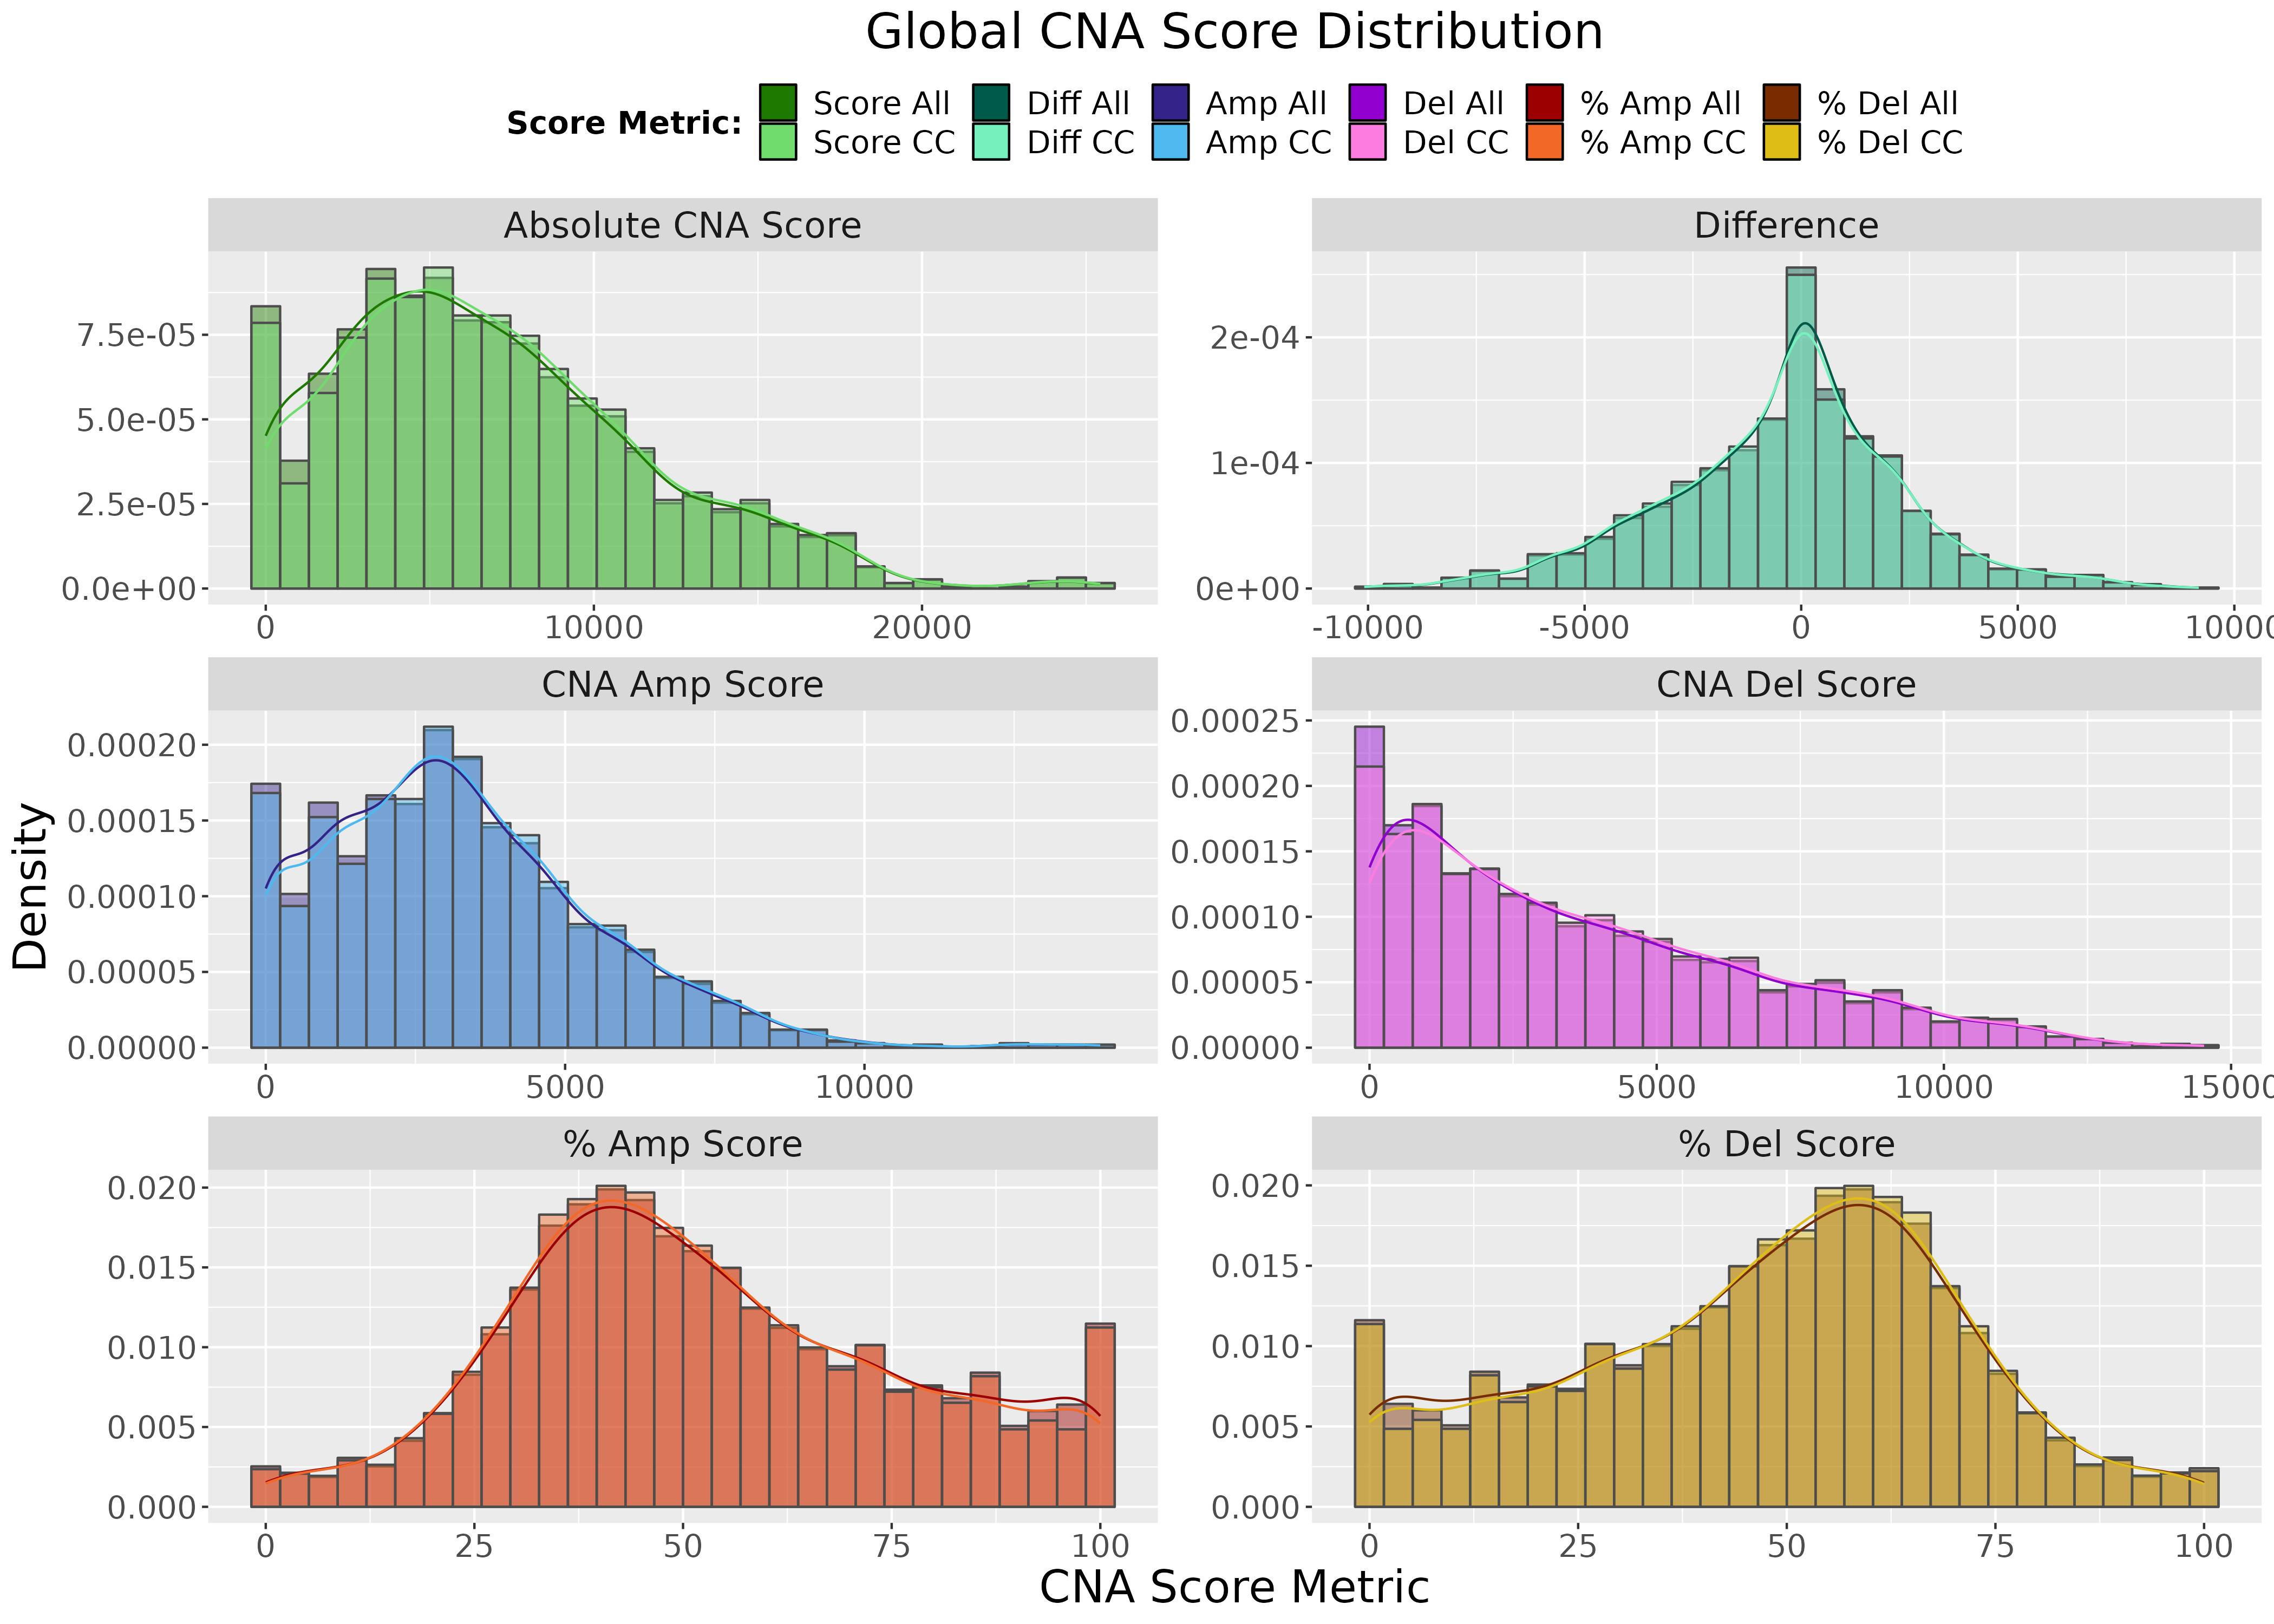
\includegraphics[width = 1\textwidth]{../figures/Chapter_2/Global_CNA_Score_Comparative_Density.png}
\caption[Density plots for each global CNA Score metric.]{Density plots for each global CNA Score metric. Each facet contains density plots for both the complete-case CNA Score metric and the CNA Score metric calculated using all available data.}
\label{fig:Score_Comp_Dense}
\end{figure}
\vfill 

\begin{figure}[!htb]
\center
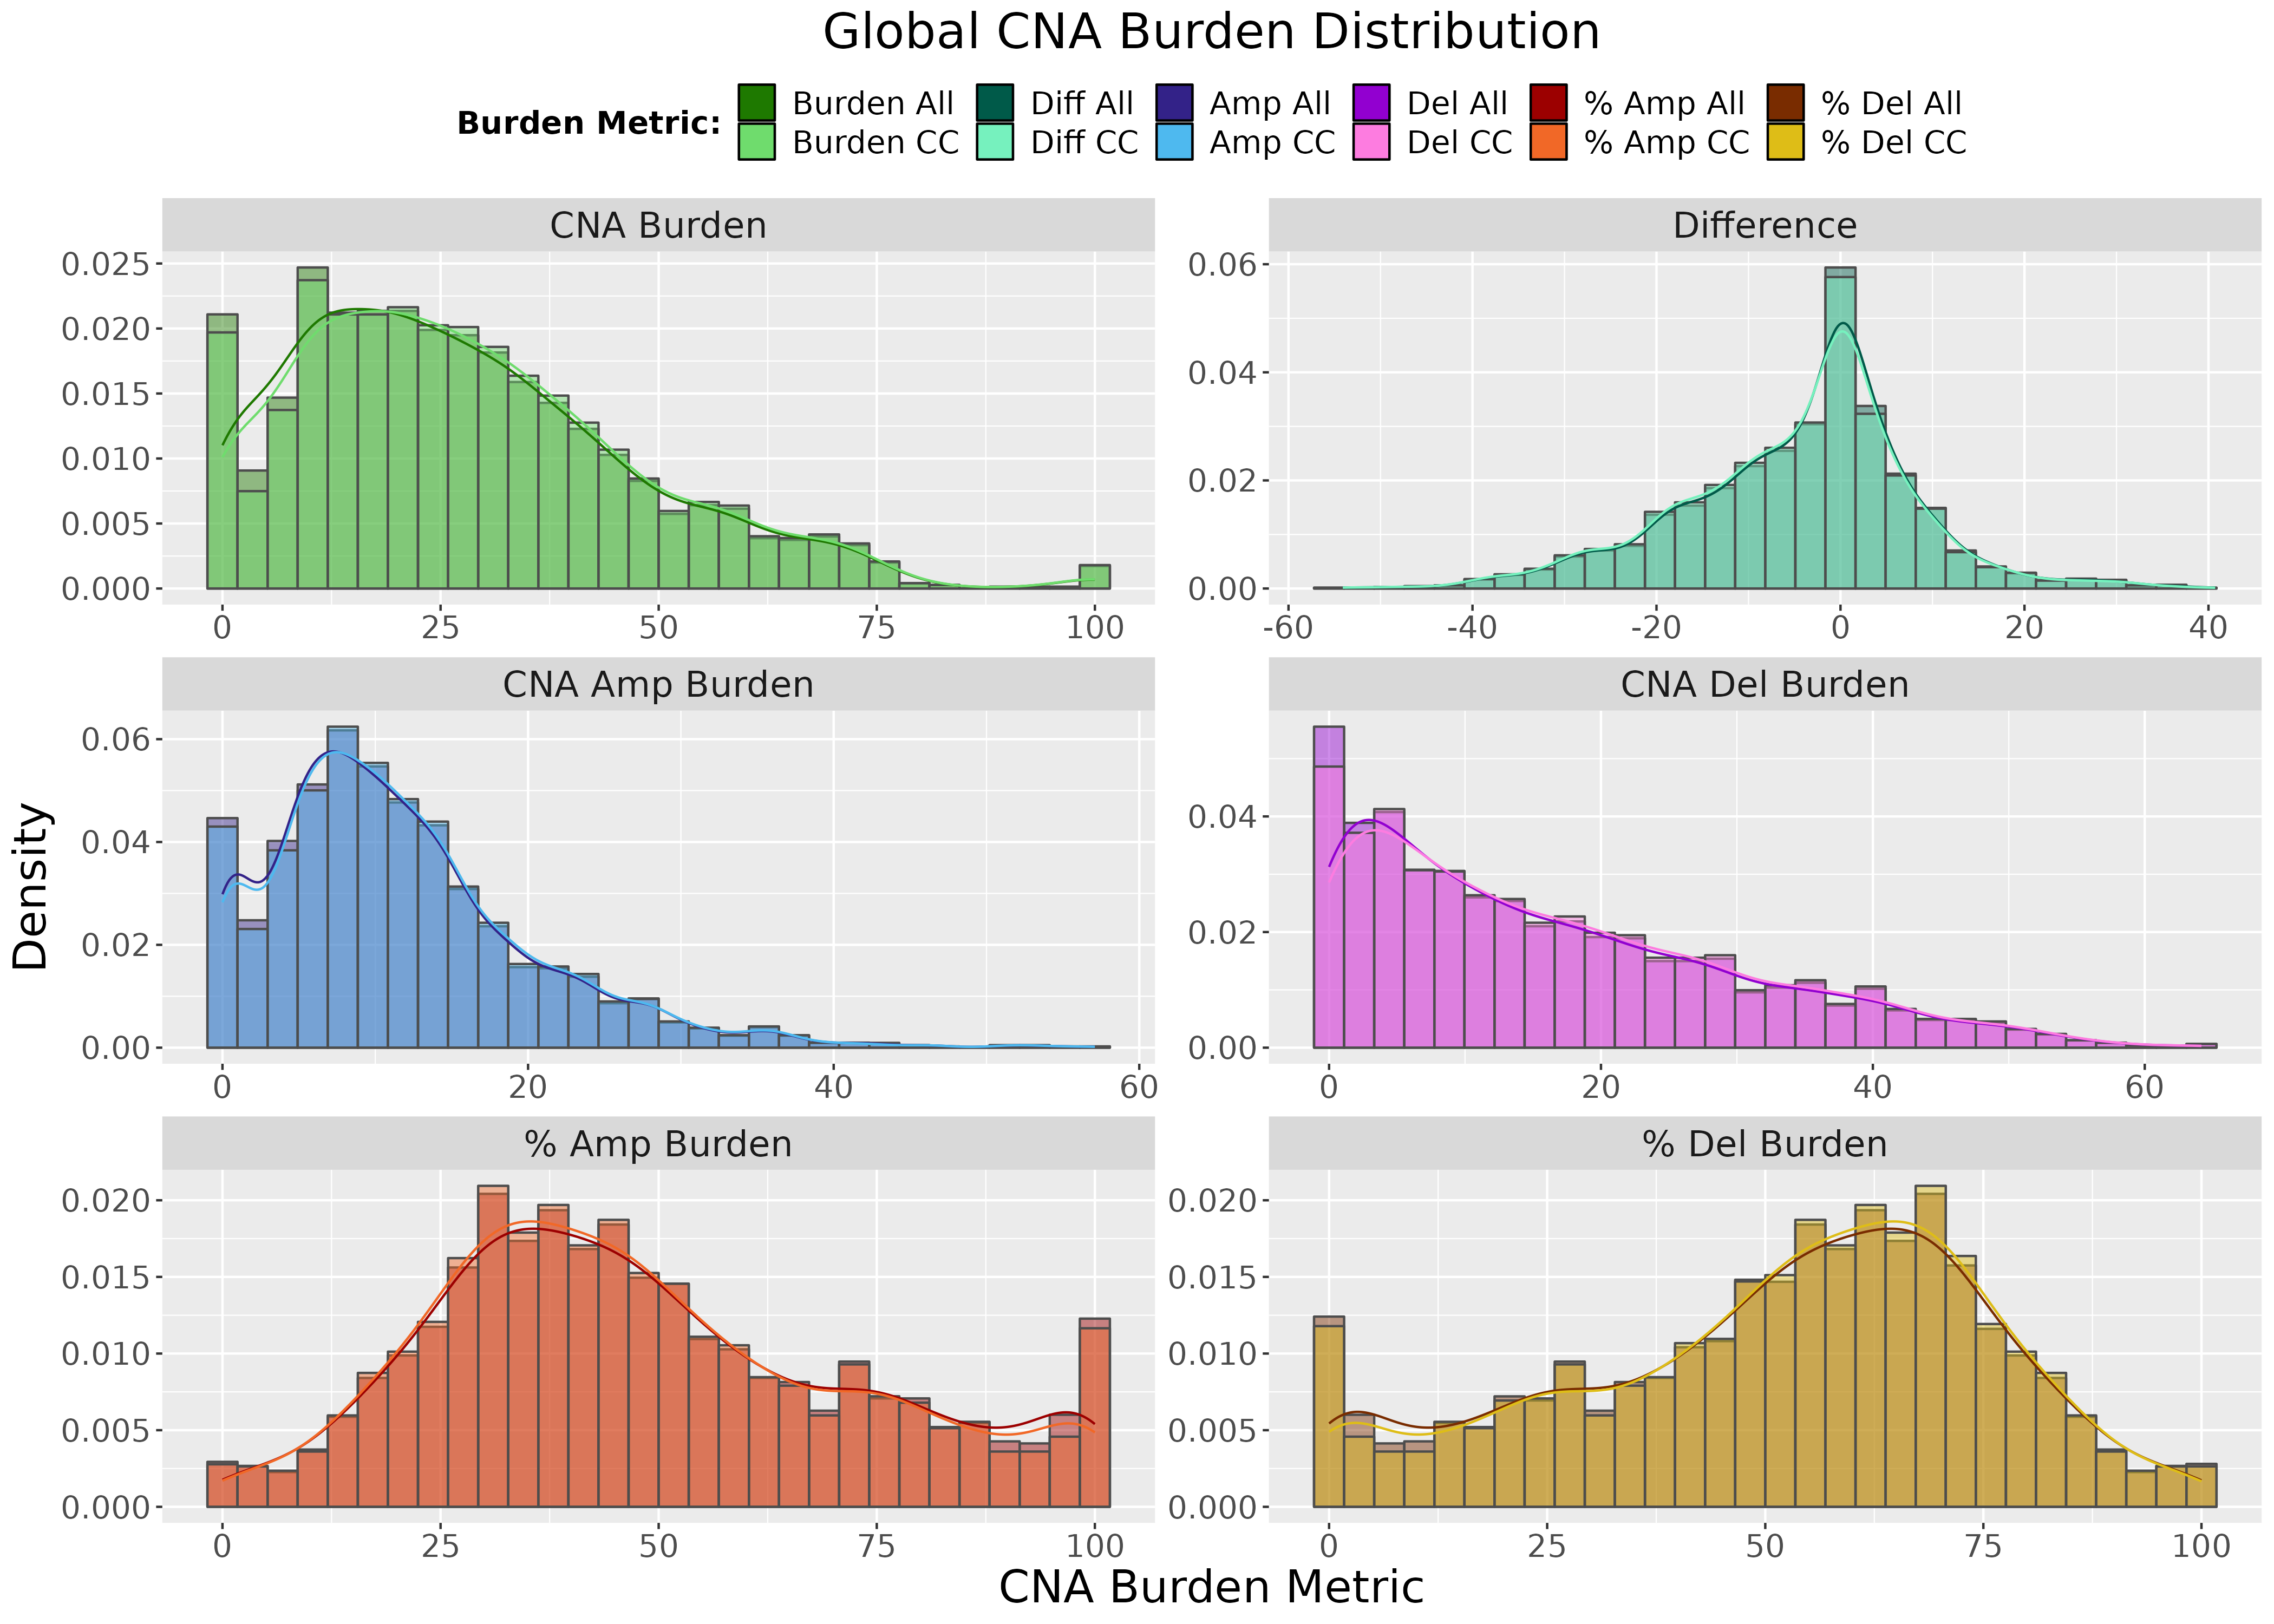
\includegraphics[width = 1\textwidth]{../figures/Chapter_2/Global_CNA_Burden_Comparative_Density.png}
\caption[Density plots for each global CNA Burden metric.]{Density plots for each global CNA Burden metric. Each facet contains density plots for both the complete-case CNA Burden metric and the CNA Burden metric calculated using all available data.}
\label{fig:Burden_Comp_Dense}
\end{figure}

\begin{table}[!htb]
\center
\caption[Summary statistics of the CNA Score metrics where all available data are used.]{Summary statistics of the CNA Score metrics where all available data are used.}
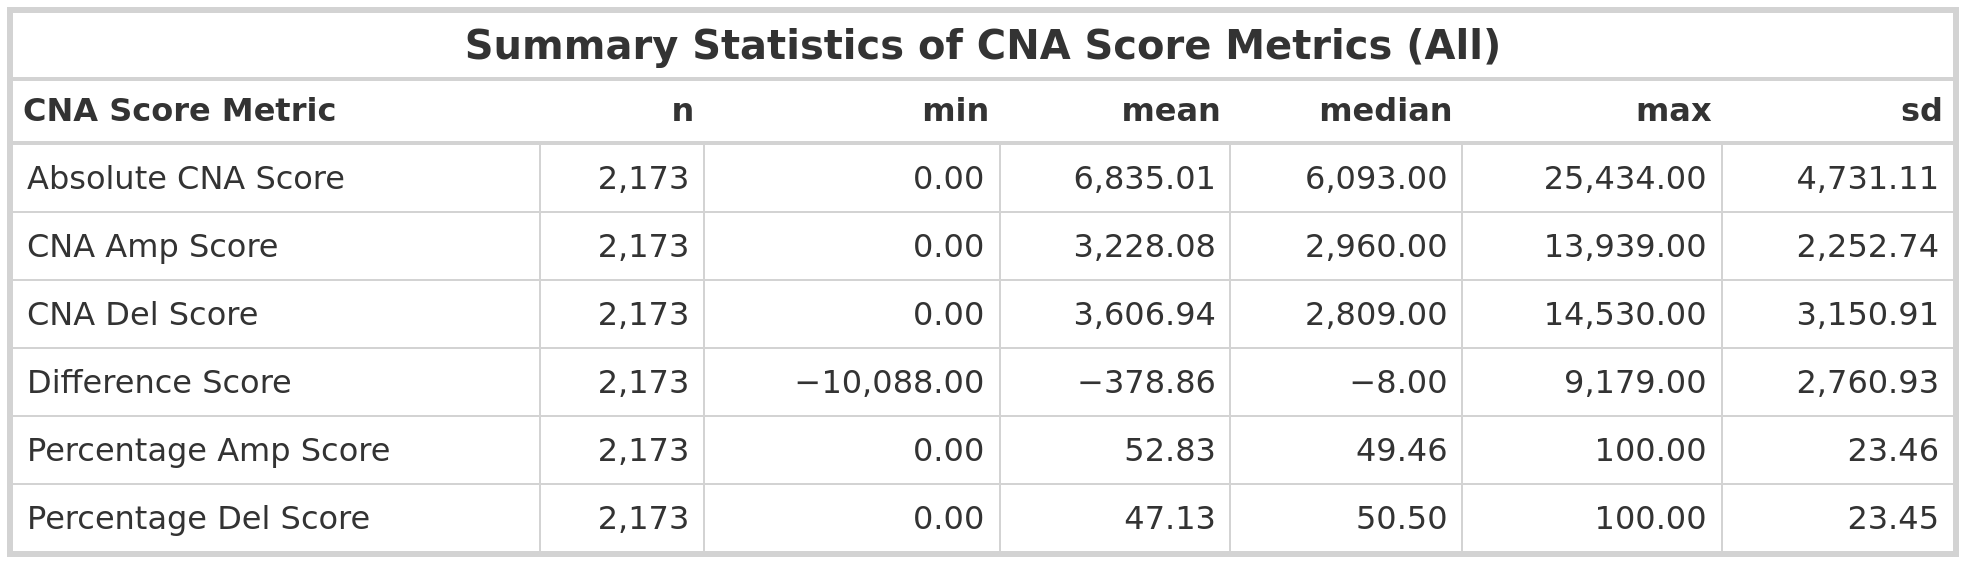
\includegraphics[width = 0.98\textwidth]{../tables/Chapter_2/Global_CNA_Score_Metric_All_Summary.png}
\label{tab:Score_All}
\end{table}

\begin{table}[!htb]
\center
\caption[Summary statistics of the CNA Score metrics where only complete cases are used.]{Summary statistics of the CNA Score metrics where only complete cases are used.}
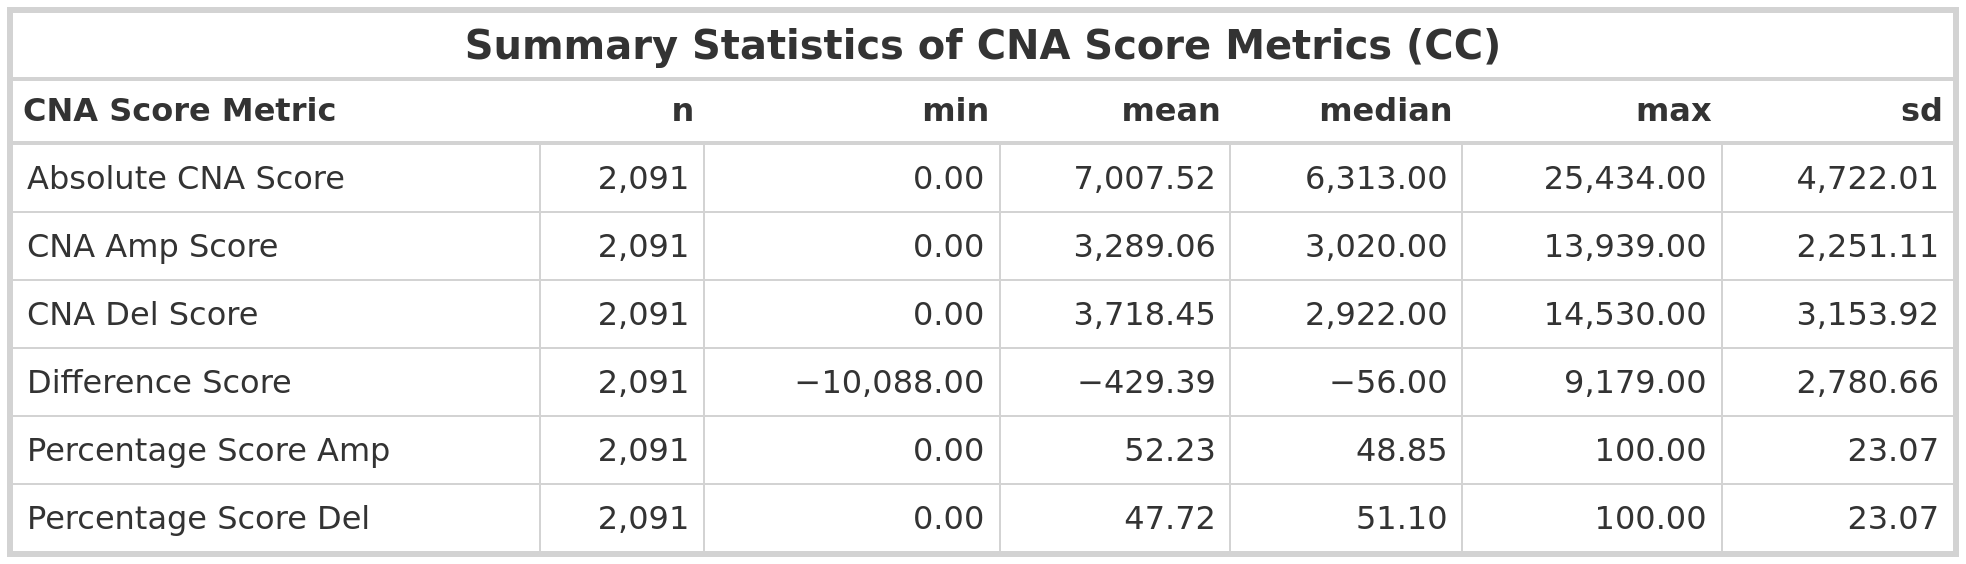
\includegraphics[width = 0.98\textwidth]{../tables/Chapter_2/Global_CNA_Score_Metric_CCA_Summary.png}
\label{tab:Score_CCA}
\end{table}

\begin{table}[!htb]
\center
\caption[Summary statistics of the CNA Burden metrics where all available data are used.]{Summary statistics of the CNA Burden metrics where all available data are used.}
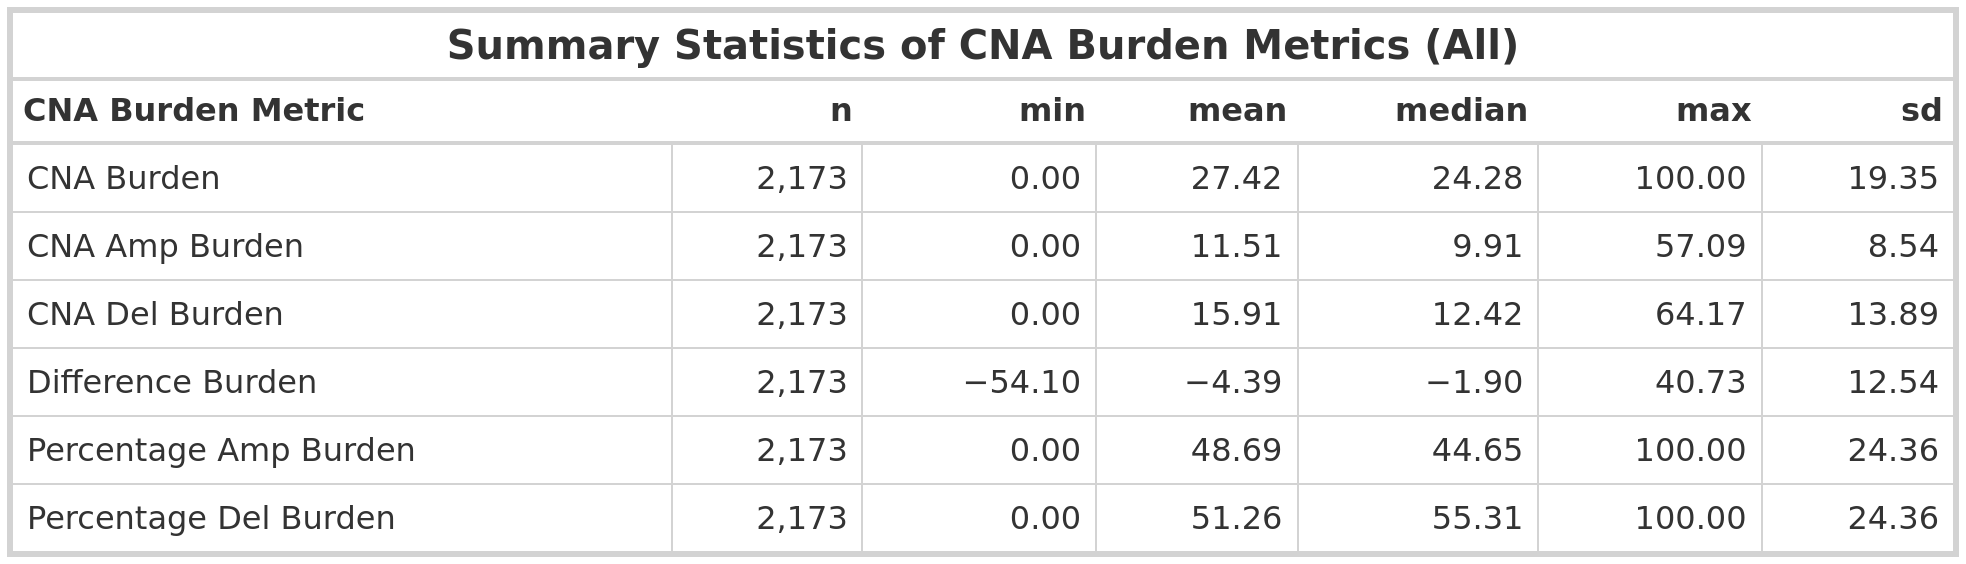
\includegraphics[width = 0.98\textwidth]{../tables/Chapter_2/Global_CNA_Burden_Metric_All_Summary.png}
\label{tab:Burden_All}
\end{table}

\begin{table}[!htb]
\center
\caption[Summary statistics of the CNA Burden metrics where only complete cases are used.]{Summary statistics of the CNA Burden metrics where only complete cases are used.}
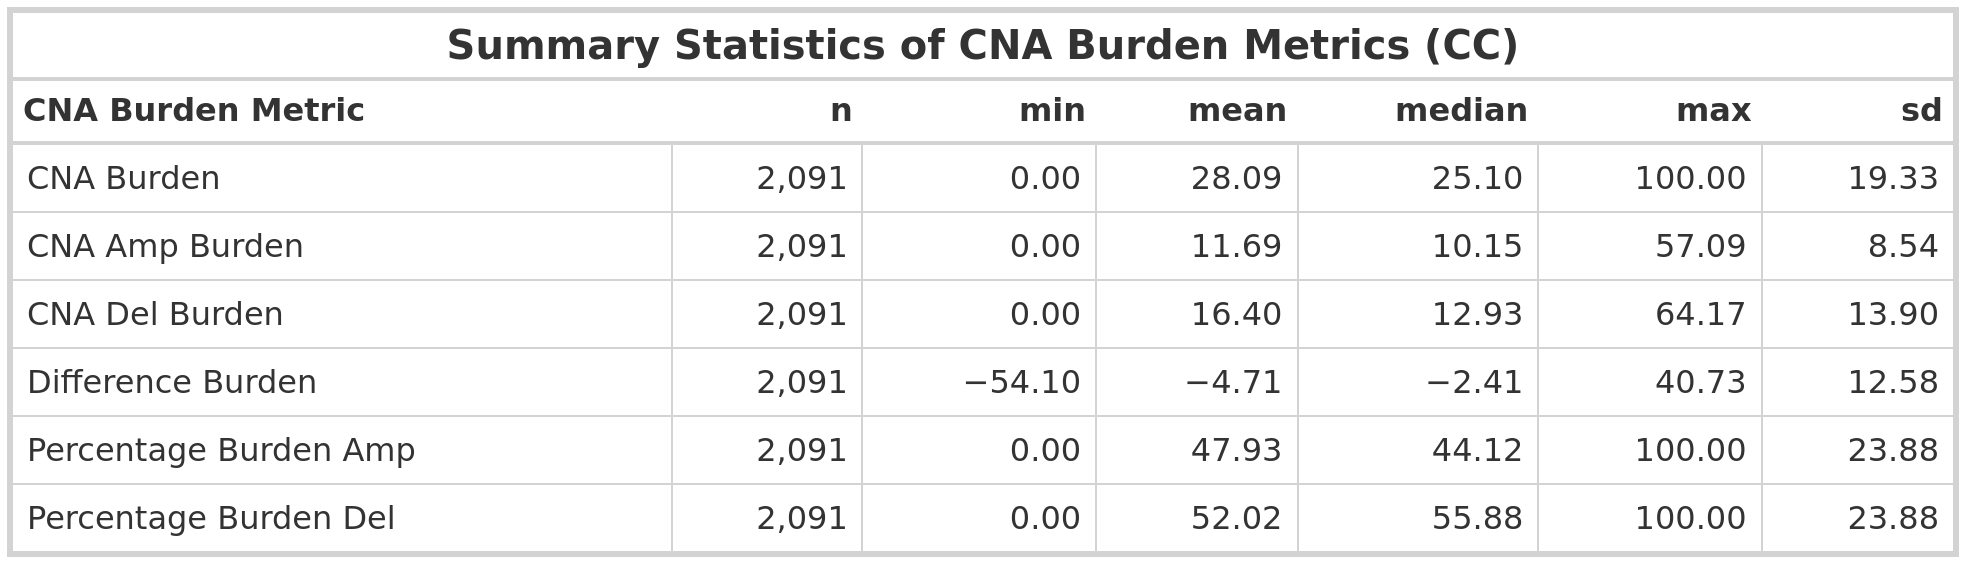
\includegraphics[width = 0.98\textwidth]{../tables/Chapter_2/Global_CNA_Burden_Metric_CCA_Summary.png}
\label{tab:Burden_CCA}
\end{table}

\begin{table}[h]
    \begin{minipage}{.49\linewidth}
    \caption[The percentage overlap between the global complete-case and all-case CNA Score metric densities]{
    The percentage overlap between the global complete-case and all-case CNA Score metric densities.
    Metrics are ordered and coloured by percentage overlap.}
      \centering 
\begin{tabular}[t]{l>{}r}
\toprule
CNA Score Metric & \% Overlap\\
\midrule
Absolute CNA Score & \cellcolor[HTML]{414487}{\textcolor{white}{96.55}}\\
 
CNA Del Score & \cellcolor[HTML]{482374}{\textcolor{white}{97.15}}\\
 
CNA Amp Score & \cellcolor[HTML]{481769}{\textcolor{white}{97.35}}\\
 
\% CNA Score Amp & \cellcolor[HTML]{46085B}{\textcolor{white}{97.58}}\\
 
\% CNA Score Del & \cellcolor[HTML]{440154}{\textcolor{white}{97.69}}\\
 
Difference Score & \cellcolor[HTML]{440154}{\textcolor{white}{97.69}}\\
\bottomrule
\end{tabular} \label{table:CNAScoreT1}
    \end{minipage}%
    \hspace{0.4cm}
    \begin{minipage}{.49\linewidth}
      \centering
    \caption[The percentage overlap between the global complete-case and all-case CNA Burden metric densities.]{
    The percentage overlap between the global complete-case and all-case CNA Burden metric densities.
    Metrics are ordered and coloured by percentage overlap.} 
\begin{tabular}[t]{l>{}r}
\toprule
CNA Burden Metric & \% Overlap\\
\midrule
CNA Burden & \cellcolor[HTML]{414487}{\textcolor{white}{96.76}}\\
 
CNA Del Burden & \cellcolor[HTML]{472D7B}{\textcolor{white}{97.18}}\\
 
CNA Amp Burden & \cellcolor[HTML]{482979}{\textcolor{white}{97.24}}\\
 
\% CNA Burden Amp & \cellcolor[HTML]{481C6E}{\textcolor{white}{97.45}}\\
 
\% CNA Burden Del & \cellcolor[HTML]{481C6E}{\textcolor{white}{97.45}}\\
 
Difference Burden & \cellcolor[HTML]{440154}{\textcolor{white}{97.87}}\\
\bottomrule
\end{tabular} \label{table:CNABurdenT1}
    \end{minipage}
\end{table}
\clearpage

\subsubsection{Observed Distributions for Chromosome Arm CNA Metrics}  
Similarly, the observed distributions for the chromosome arm CNA metrics are inspected and an assessment of the effects of missingness is carried out. Figures \ref{SurvTrees_Score_HM_CCA} and \ref{SurvTrees_Score_HM} display the heatmaps of the chromosome arm CNA Amp and Del Score metrics calculated using compete cases only and all available data, the grey indicates missing data. Figures \ref{SurvTrees_Burden_HM_CCA} and \ref{SurvTrees_Burden_HM} display the heatmaps of the chromosome arm CNA Amp and Del Burden metrics calculated using compete cases only and all available data. Comparing A and B in each of these figures, it is observed that similar clusters of patients are generated based on both the all-case and CC chromosome arm CNA metrics. When comparing the overlap in distributions it is observed that only 10 out of the 252 chromosome arm CNA Score and Burden metrics display percentage overlap below 80\%. The lowest overlap in the CNA Score and Burden metric distributions is in the Percentage Amp metrics on 9p, 11.00\% and 10.84\%, respectively (Table \ref{table:CNAScoreT2} and \ref{table:CNABurdenT2}). The second and third lowest overlap between the CC and all-case CNA Score and Burden metric distributions is observed for chromosome arms 9p, 16.69\% and 16.83\%, and 7p, 42.65\% and 45.26\%. Density plots, focusing on chromosome 9p and 7p, are provided in Figure \ref{fig:Plot-PerArm-DensityPlots} and indicate that high density regions, such as those located around 0, display high levels of mismatch.  

Figures \ref{SurvTrees_Score_HM_CCA}-\ref{SurvTrees_Burden_HM} also highlight previously documented patterns of CNAs in breast cancer, including high levels of amplifications on chromosome 1q, 8q and 16p and high levels of deletions on 8p, 16q and 17p \citep{pmid20576095, pmid22522925}. Similar to the global CNA Score and Burden metrics, it appears that deletions are more widespread across the genome, affecting greater numbers of chromosomes, than amplifications. 

Rather than extensively presenting details of distributions for each of the 42 chromosome arms, we select chromosome arm 1q for more detailed illustration and discussion (see Supplementary Information for remaining chromosome arms). Chromosome arm 1q is frequently altered in breast cancer and shows interesting features in this analysis. The summary statistics (Tables \ref{tab:Score_All_Chr1q}-\ref{tab:Burden_CCA_Chr1q}) and distributions (Figures \ref{fig:Score_Comp_Dense_Chr1q} and \ref{fig:Burden_Comp_Dense_Chr1q}) indicate that the copy number landscape of chromosome 1q is dominated by amplifications, median CNA Score values 0 and 954 and median CNA Burden values 0 and 78.71\%, for deletions and amplifications, respectively. The maximum values of the CNA Burden and CNA Amp, 100\% and 99.91\%, and the Difference Score distribution being nearly entirely positive also suggests that almost all of the alterations observed are amplifications. Figure \ref{fig:Score_Comp_Dense_Chr1q} indicates that three of the CNA Score metrics on chromosome 1q, Absolute CNA Score, CNA Amp Score and Difference Score, have trimodal distributions. Three peaks correspond to cases where patients have low, moderate and high levels of GI. For the CNA Burden metrics the majority of the metric distributions are bimodal, with peaks corresponding to patients with low and high GI. 

Overall, assessing distributions of the global CNA metrics comparing CC patient data to all-patient data, i.e. including those with some missingness prevalent, shows that missing values have only a minor impact on these distributions. The impact of missingness is greater in the chromosome arm CNA metric distributions, however, as the majority of distributions displayed greater than 80\% overlap, it is determined that including all cases, across the global and chromosome arm-specific metrics, is unlikely to invoke bias in the form of underestimating the CNA metrics. Furthermore, imputation of missing CNA values was considered but not performed as the impact of the missing values on the CNA metric distributions was shown to be minor across the majority of CNA metrics.

\vfill
\begin{figure}[!h]
  \centering
   \vspace{0.4cm}
  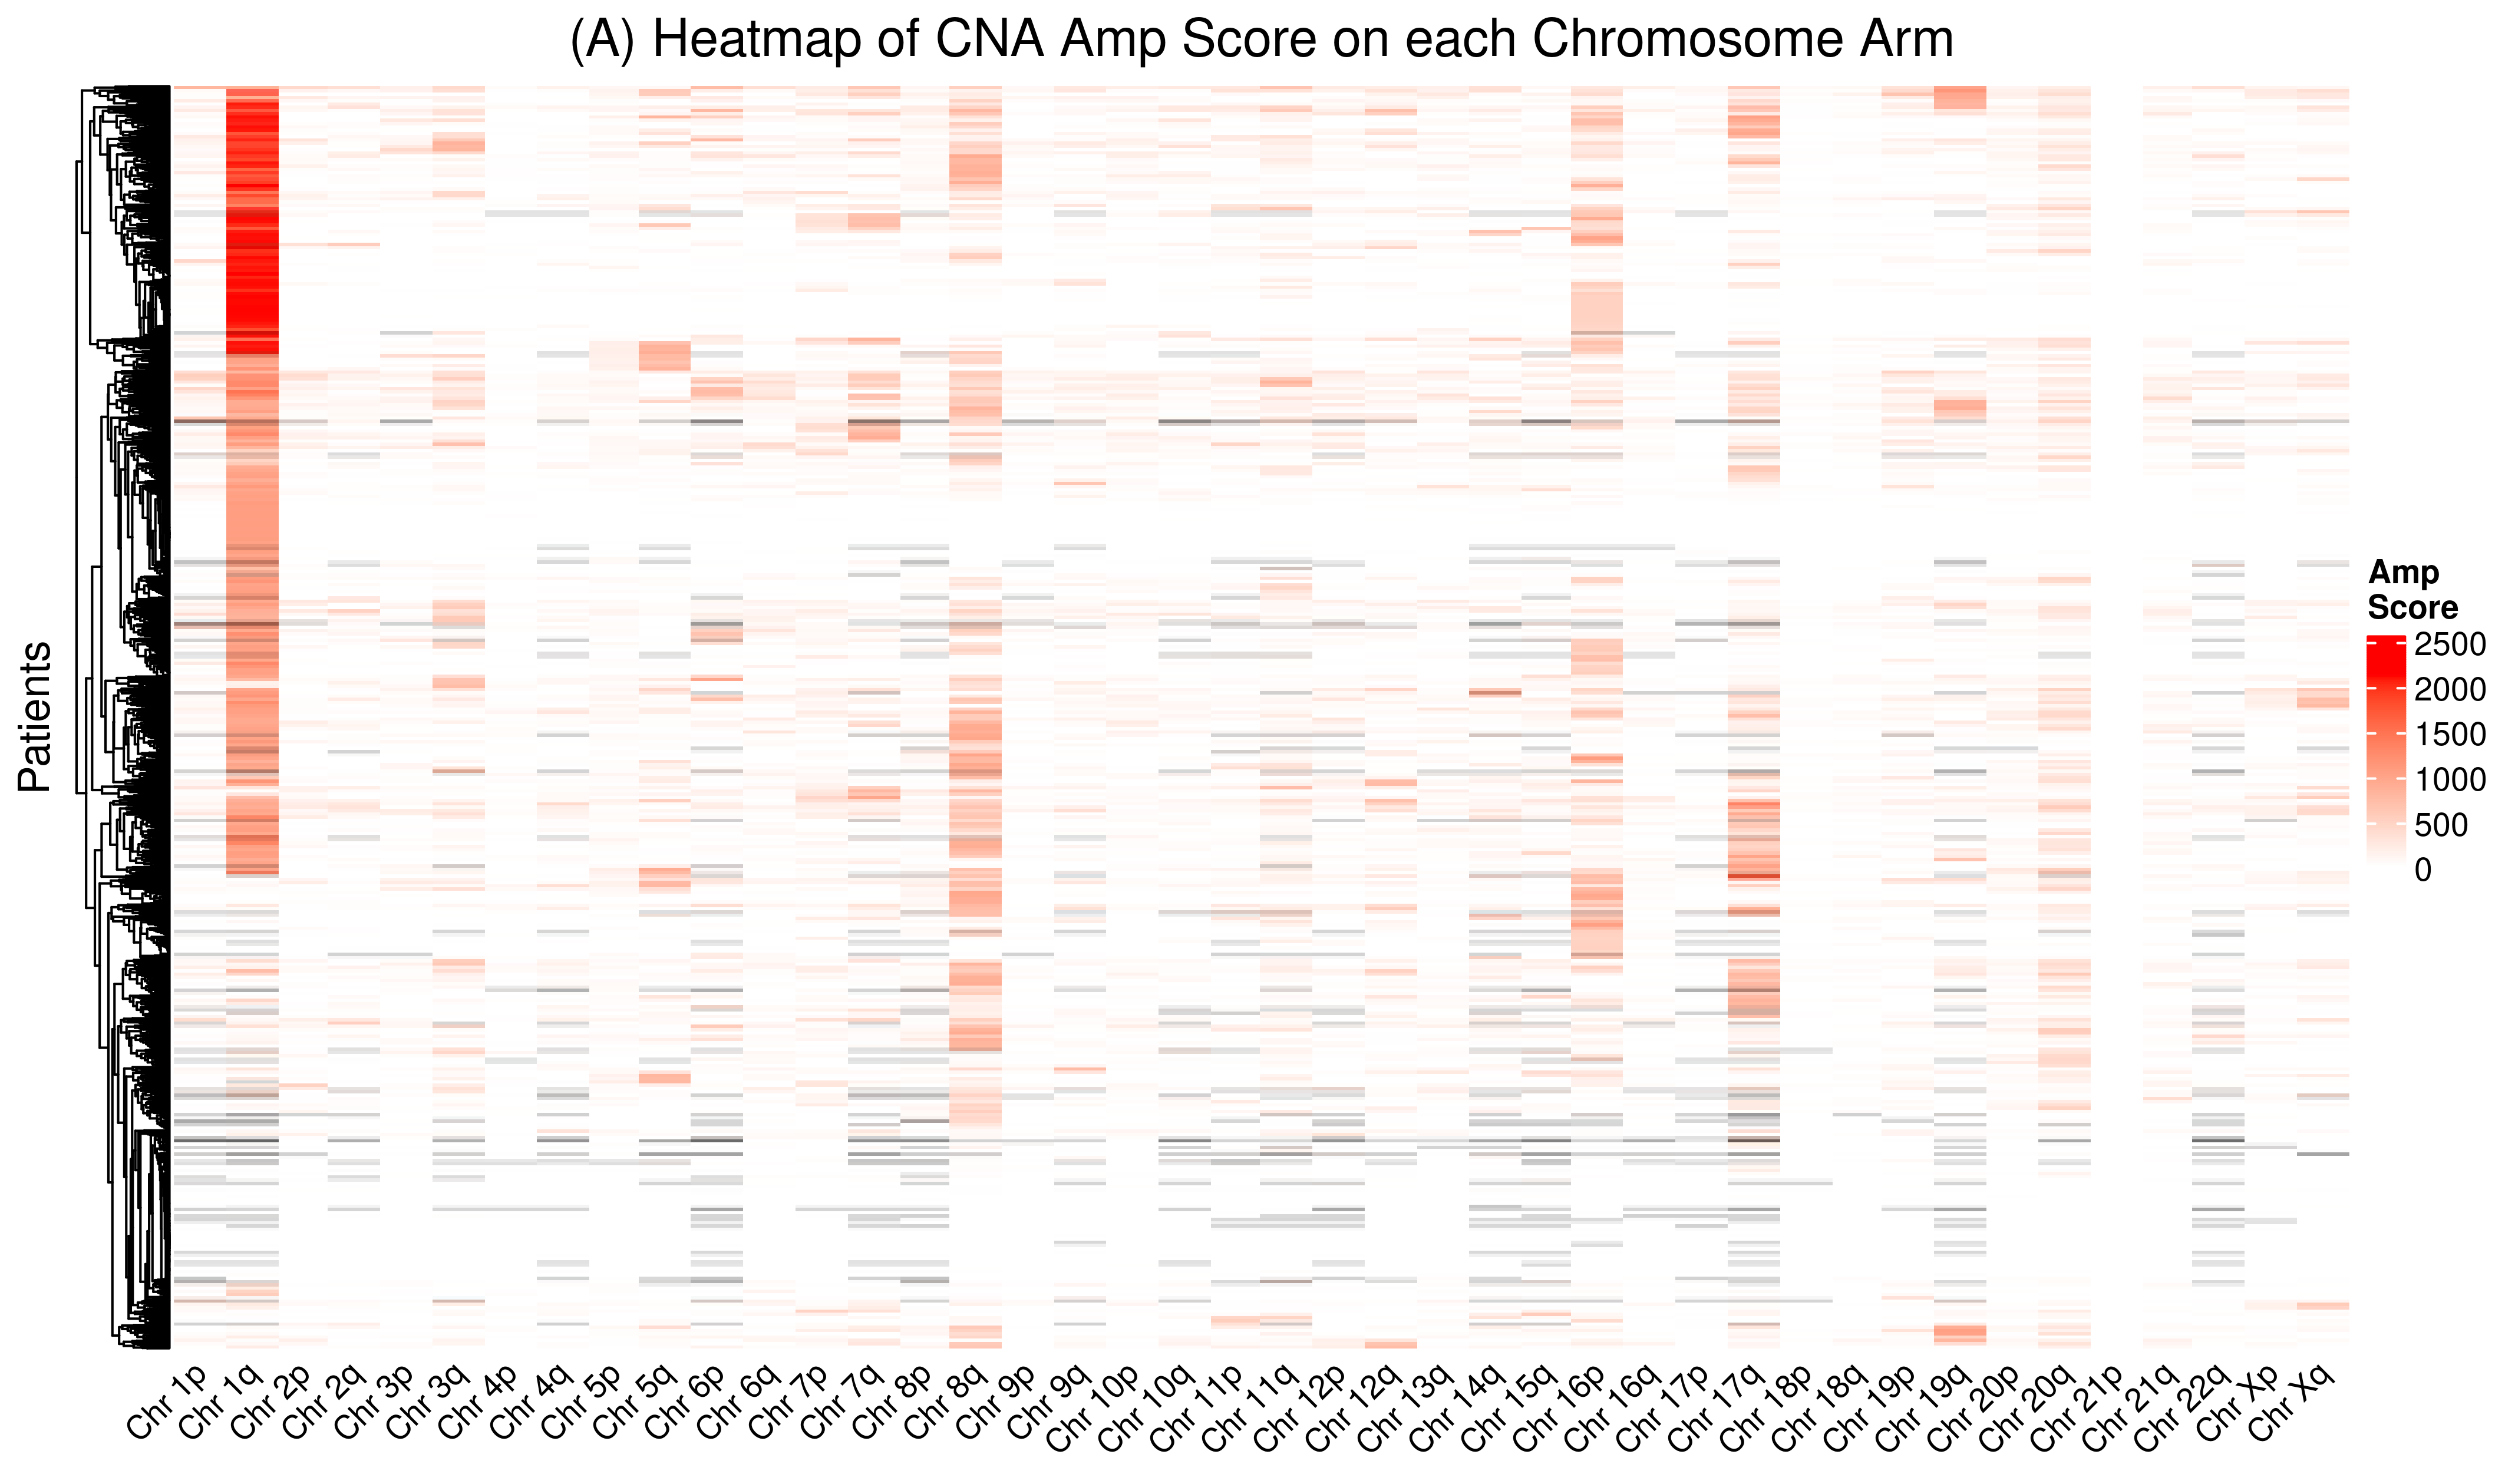
\includegraphics[width = 1.05\textwidth]{../figures/Chapter_2/CNA_Amp_Score_Heatmap_CCA.png}
  
  \vspace{1.3cm}
  
    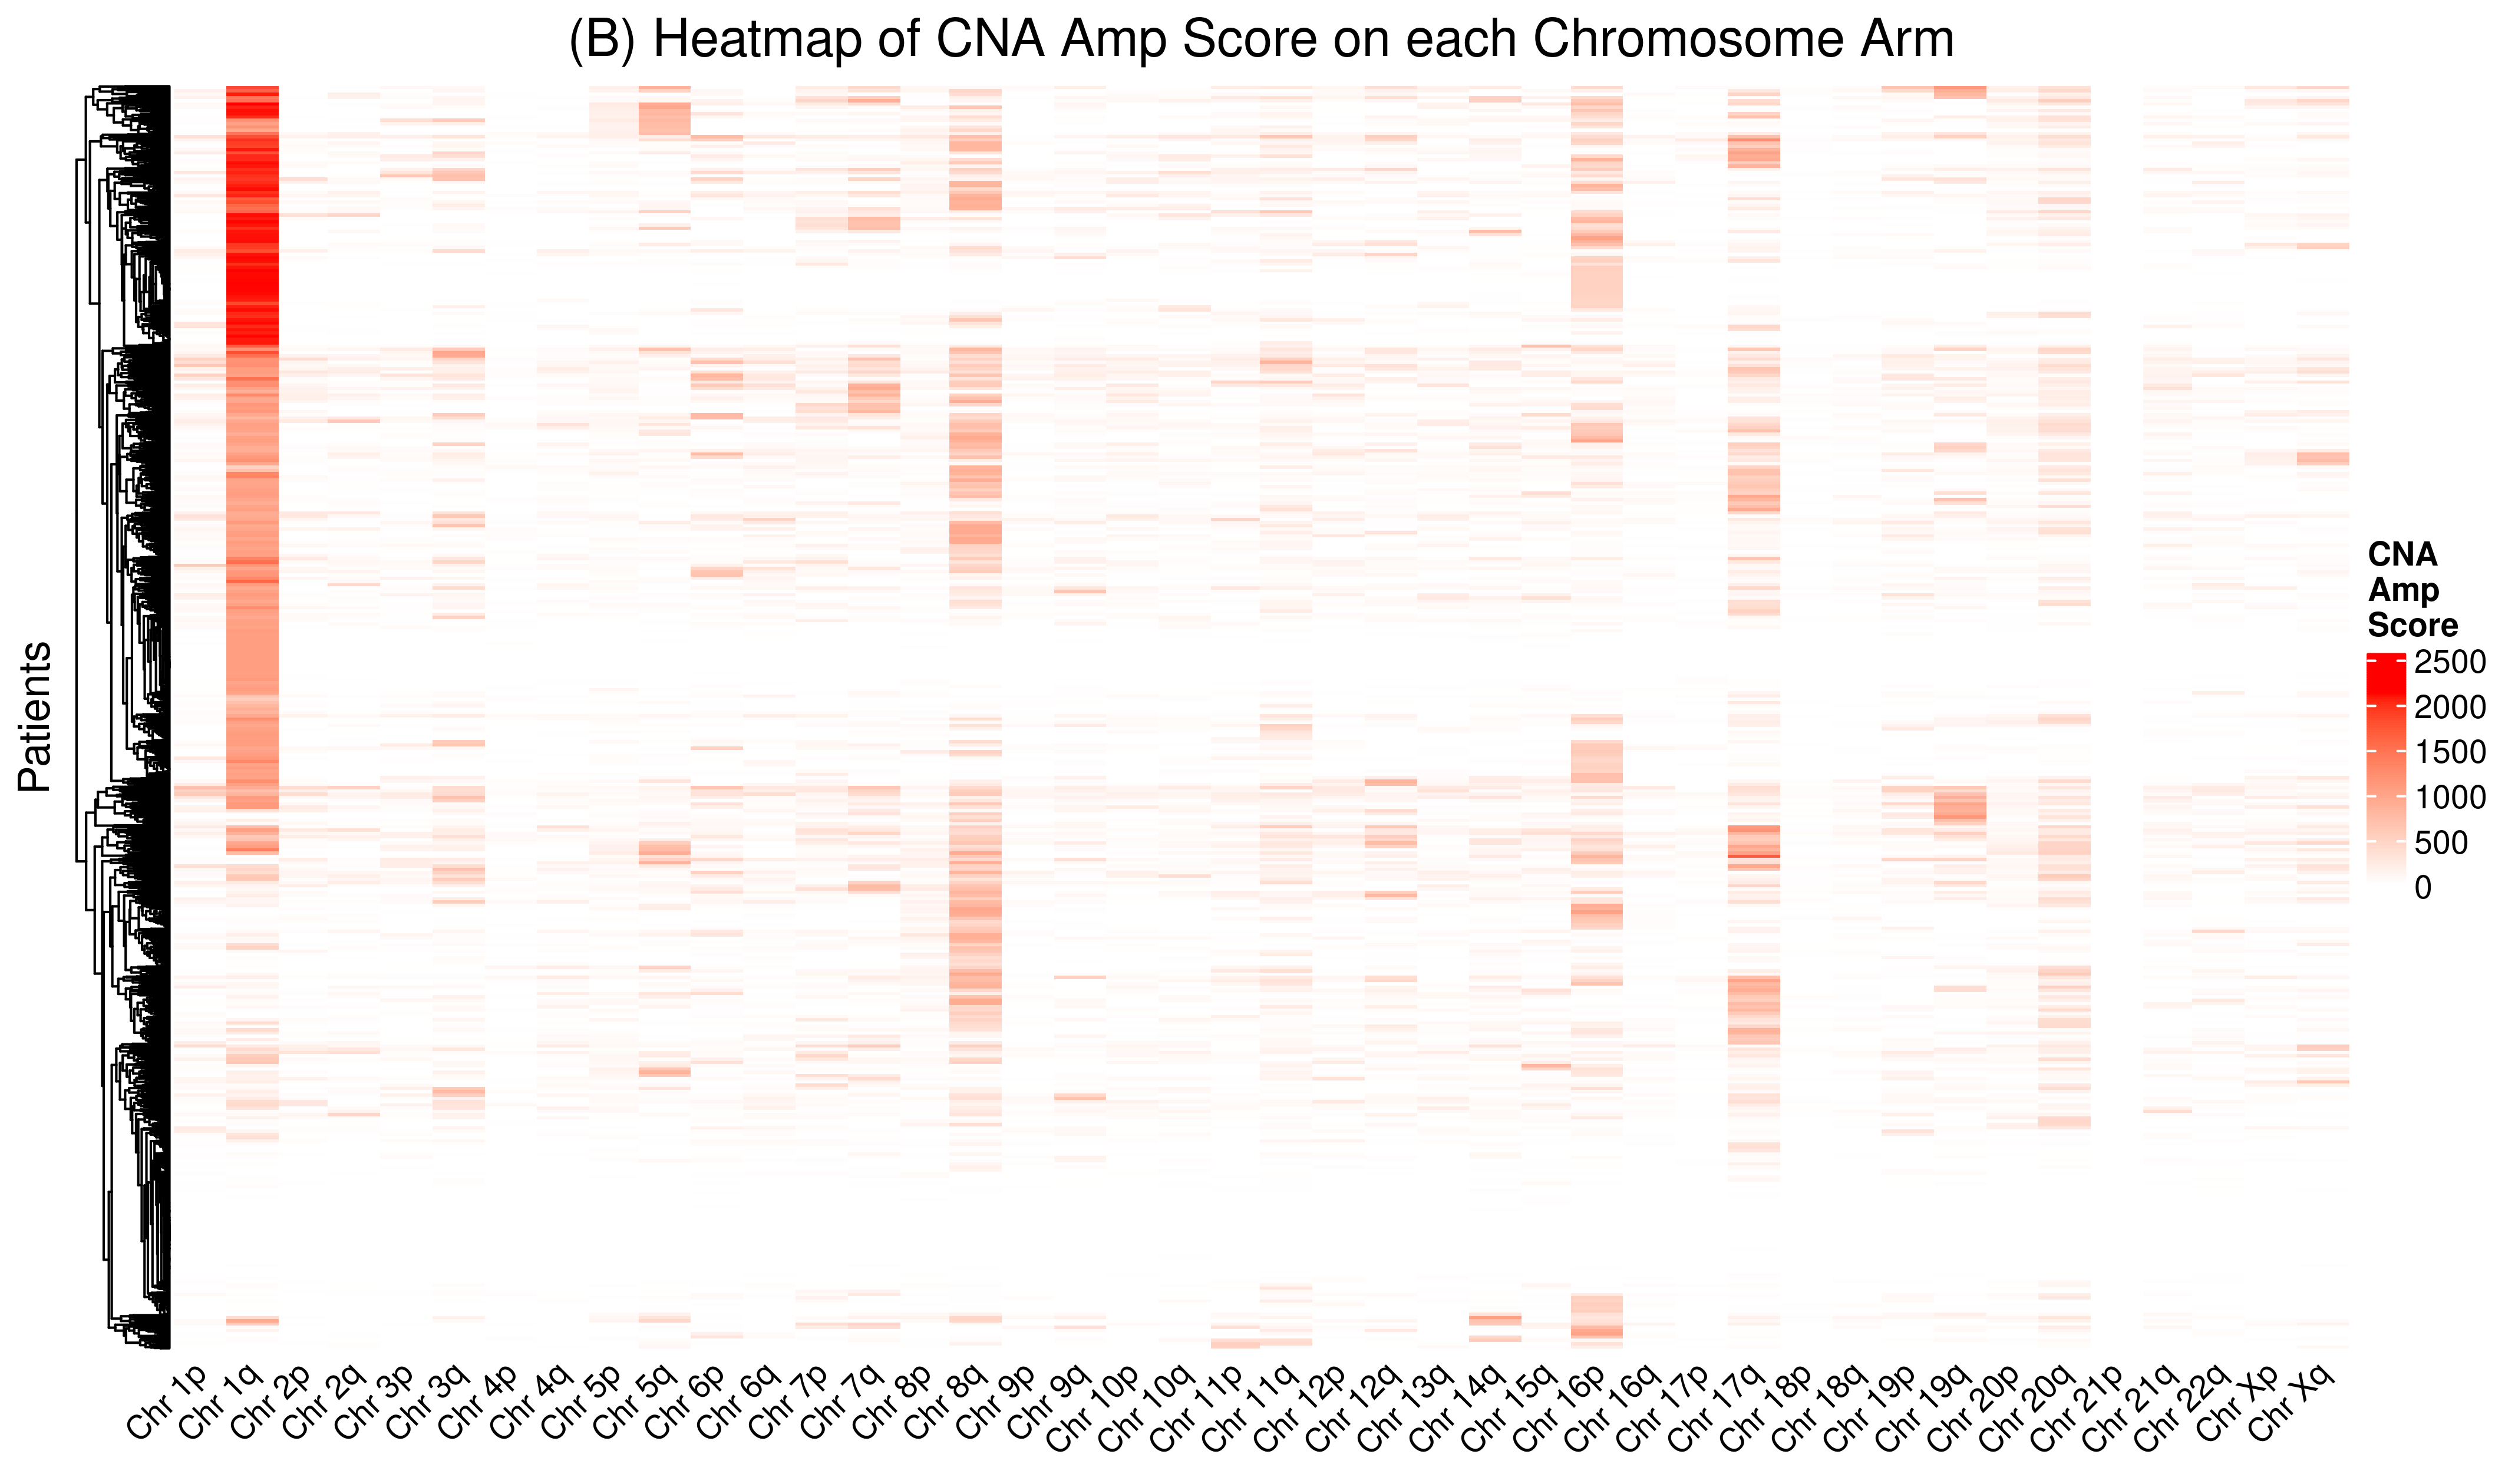
\includegraphics[width = 1.05\textwidth]{../figures/Chapter_2/CNA_Amp_Score_Heatmap_All.png}
  
   \vspace{0.4cm}
 
  \caption[Heatmap of CNA Amp Score across chromosome arms.]{Heatmap of CNA Amp Score across chromosome arms with (A) consideration to complete-case METABRIC patients only (n = 2,091) and (B) consideration to all METABRIC patients including those presenting with some missing data (n = 2,173). Grey indicates missing values.}
  \label{SurvTrees_Score_HM_CCA}
\end{figure}
\vfill 
\clearpage

\begin{figure}[!ht]
  \centering
  
  \vspace{0.8cm}
  
   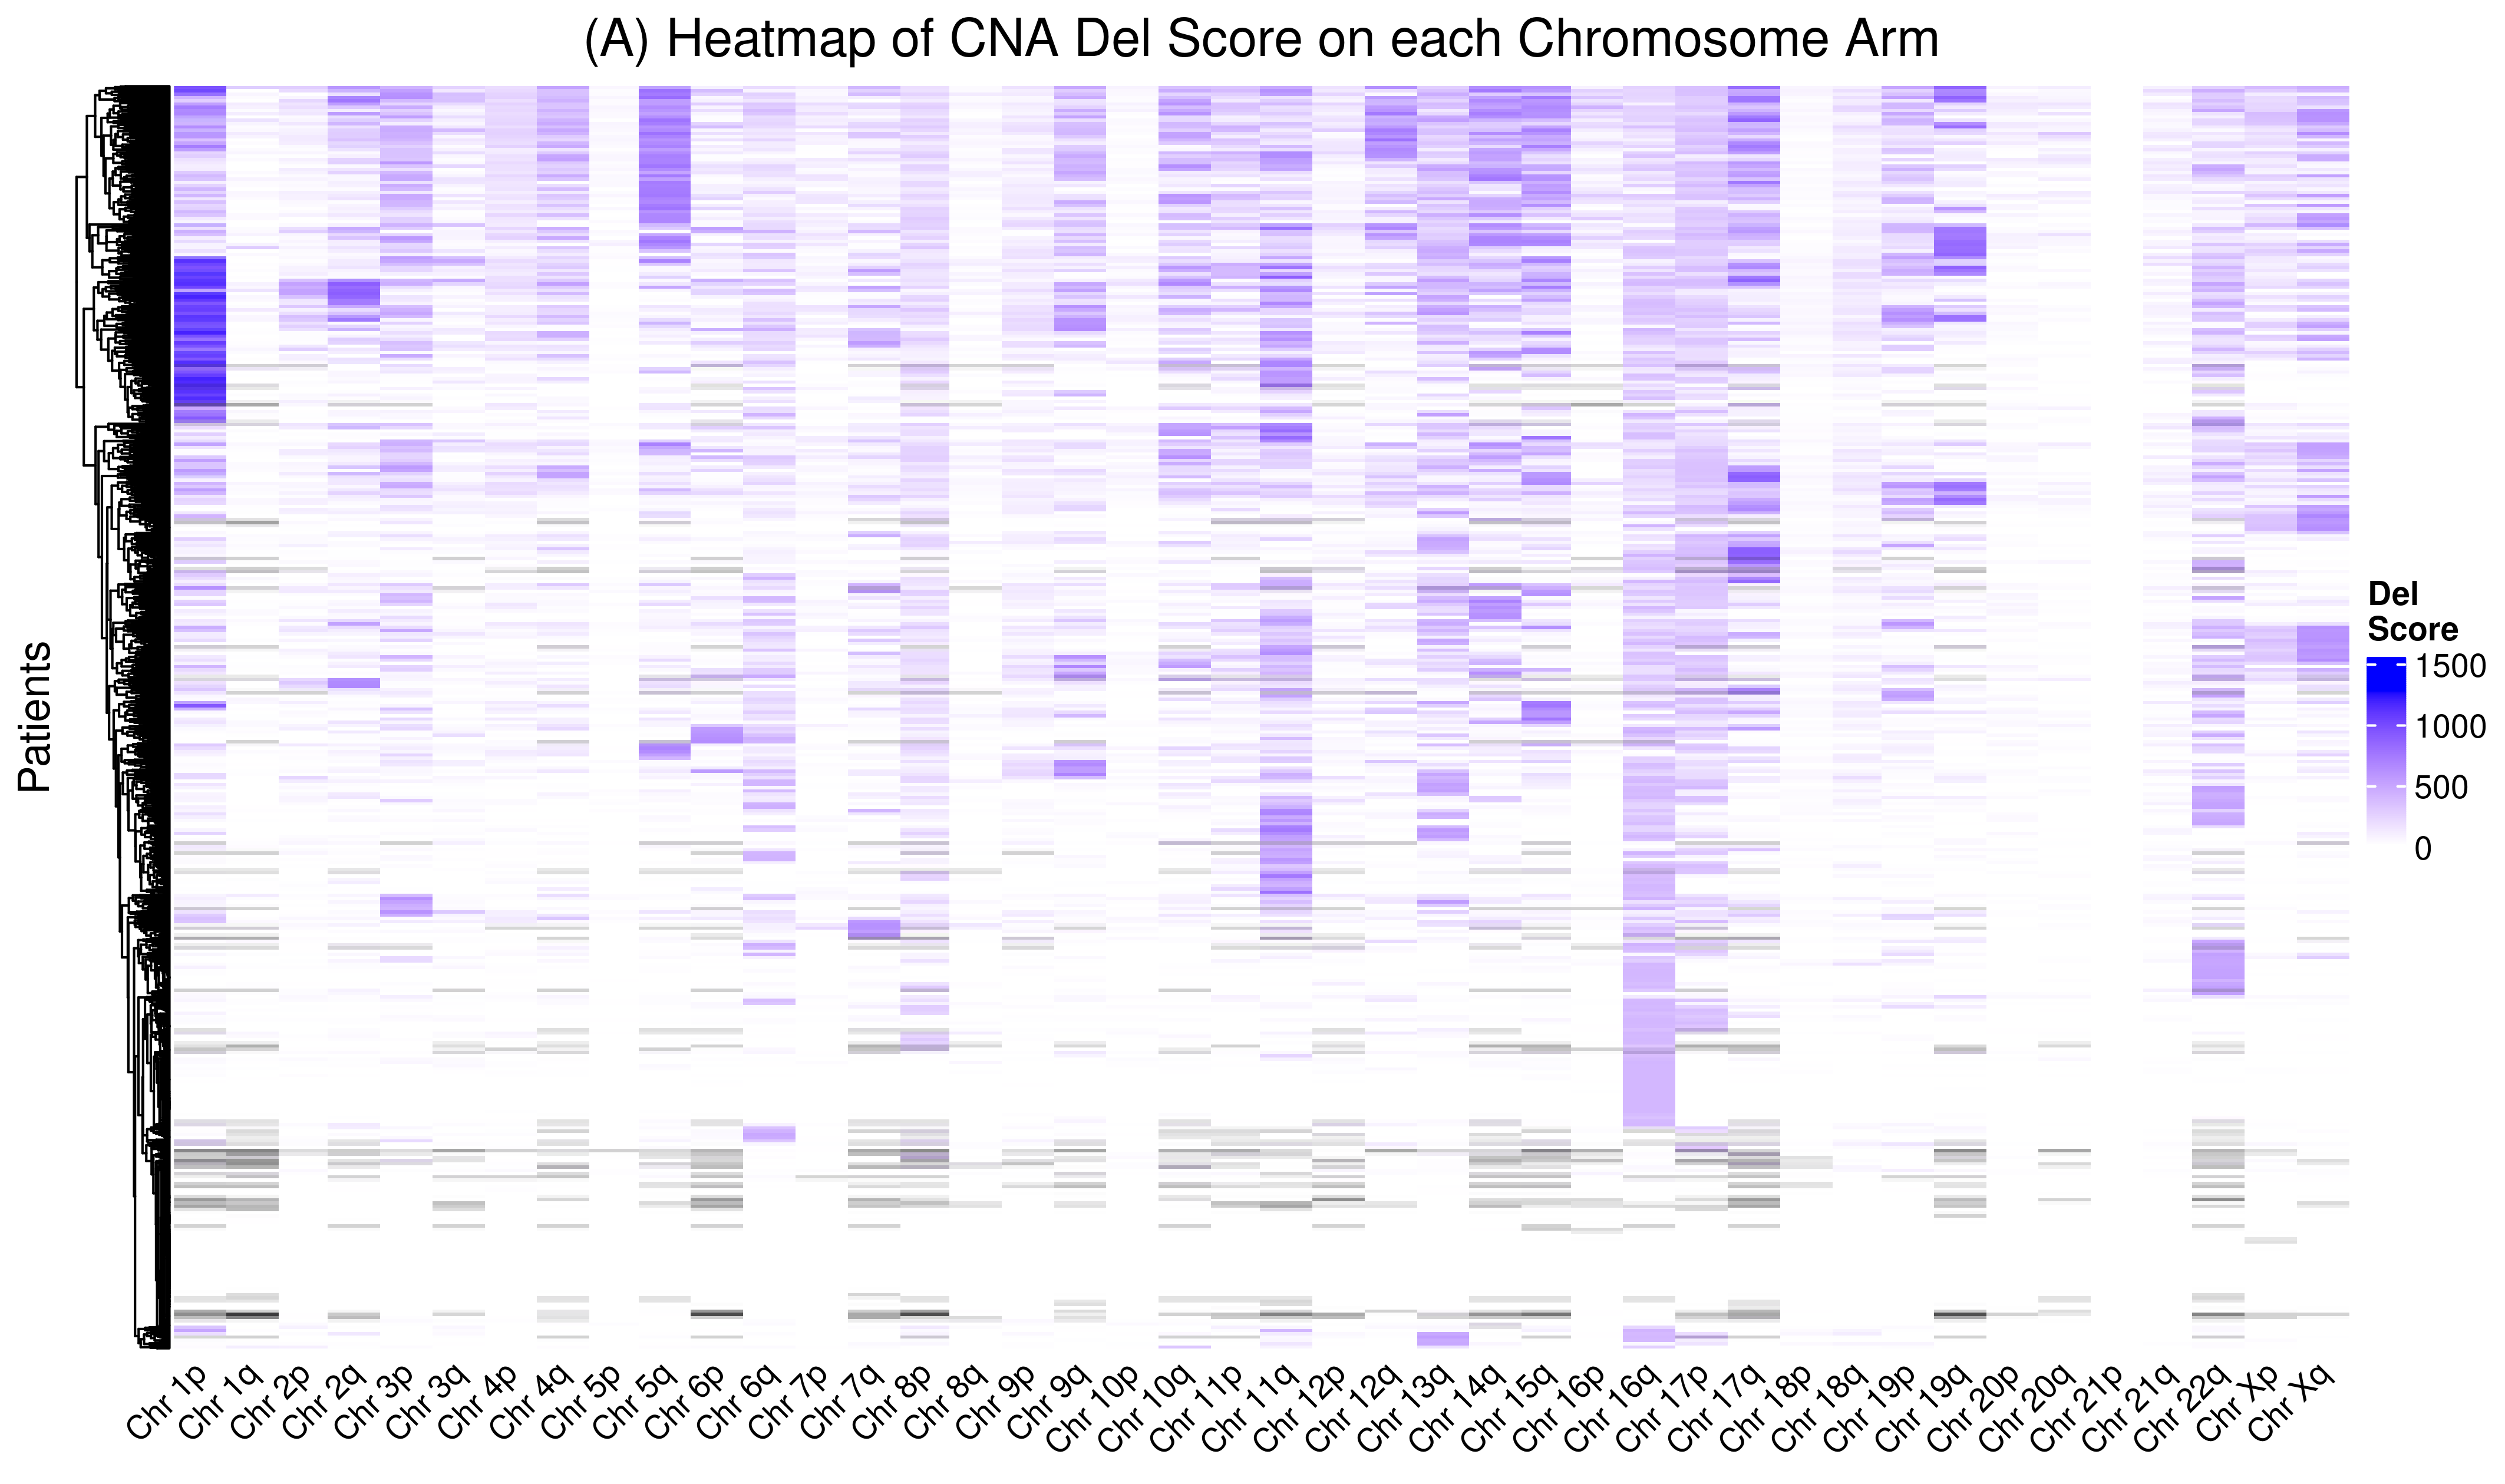
\includegraphics[width = 1.05\textwidth]{../figures/Chapter_2/CNA_Del_Score_Heatmap_CCA.png}

  \vspace{1.5cm}
   
  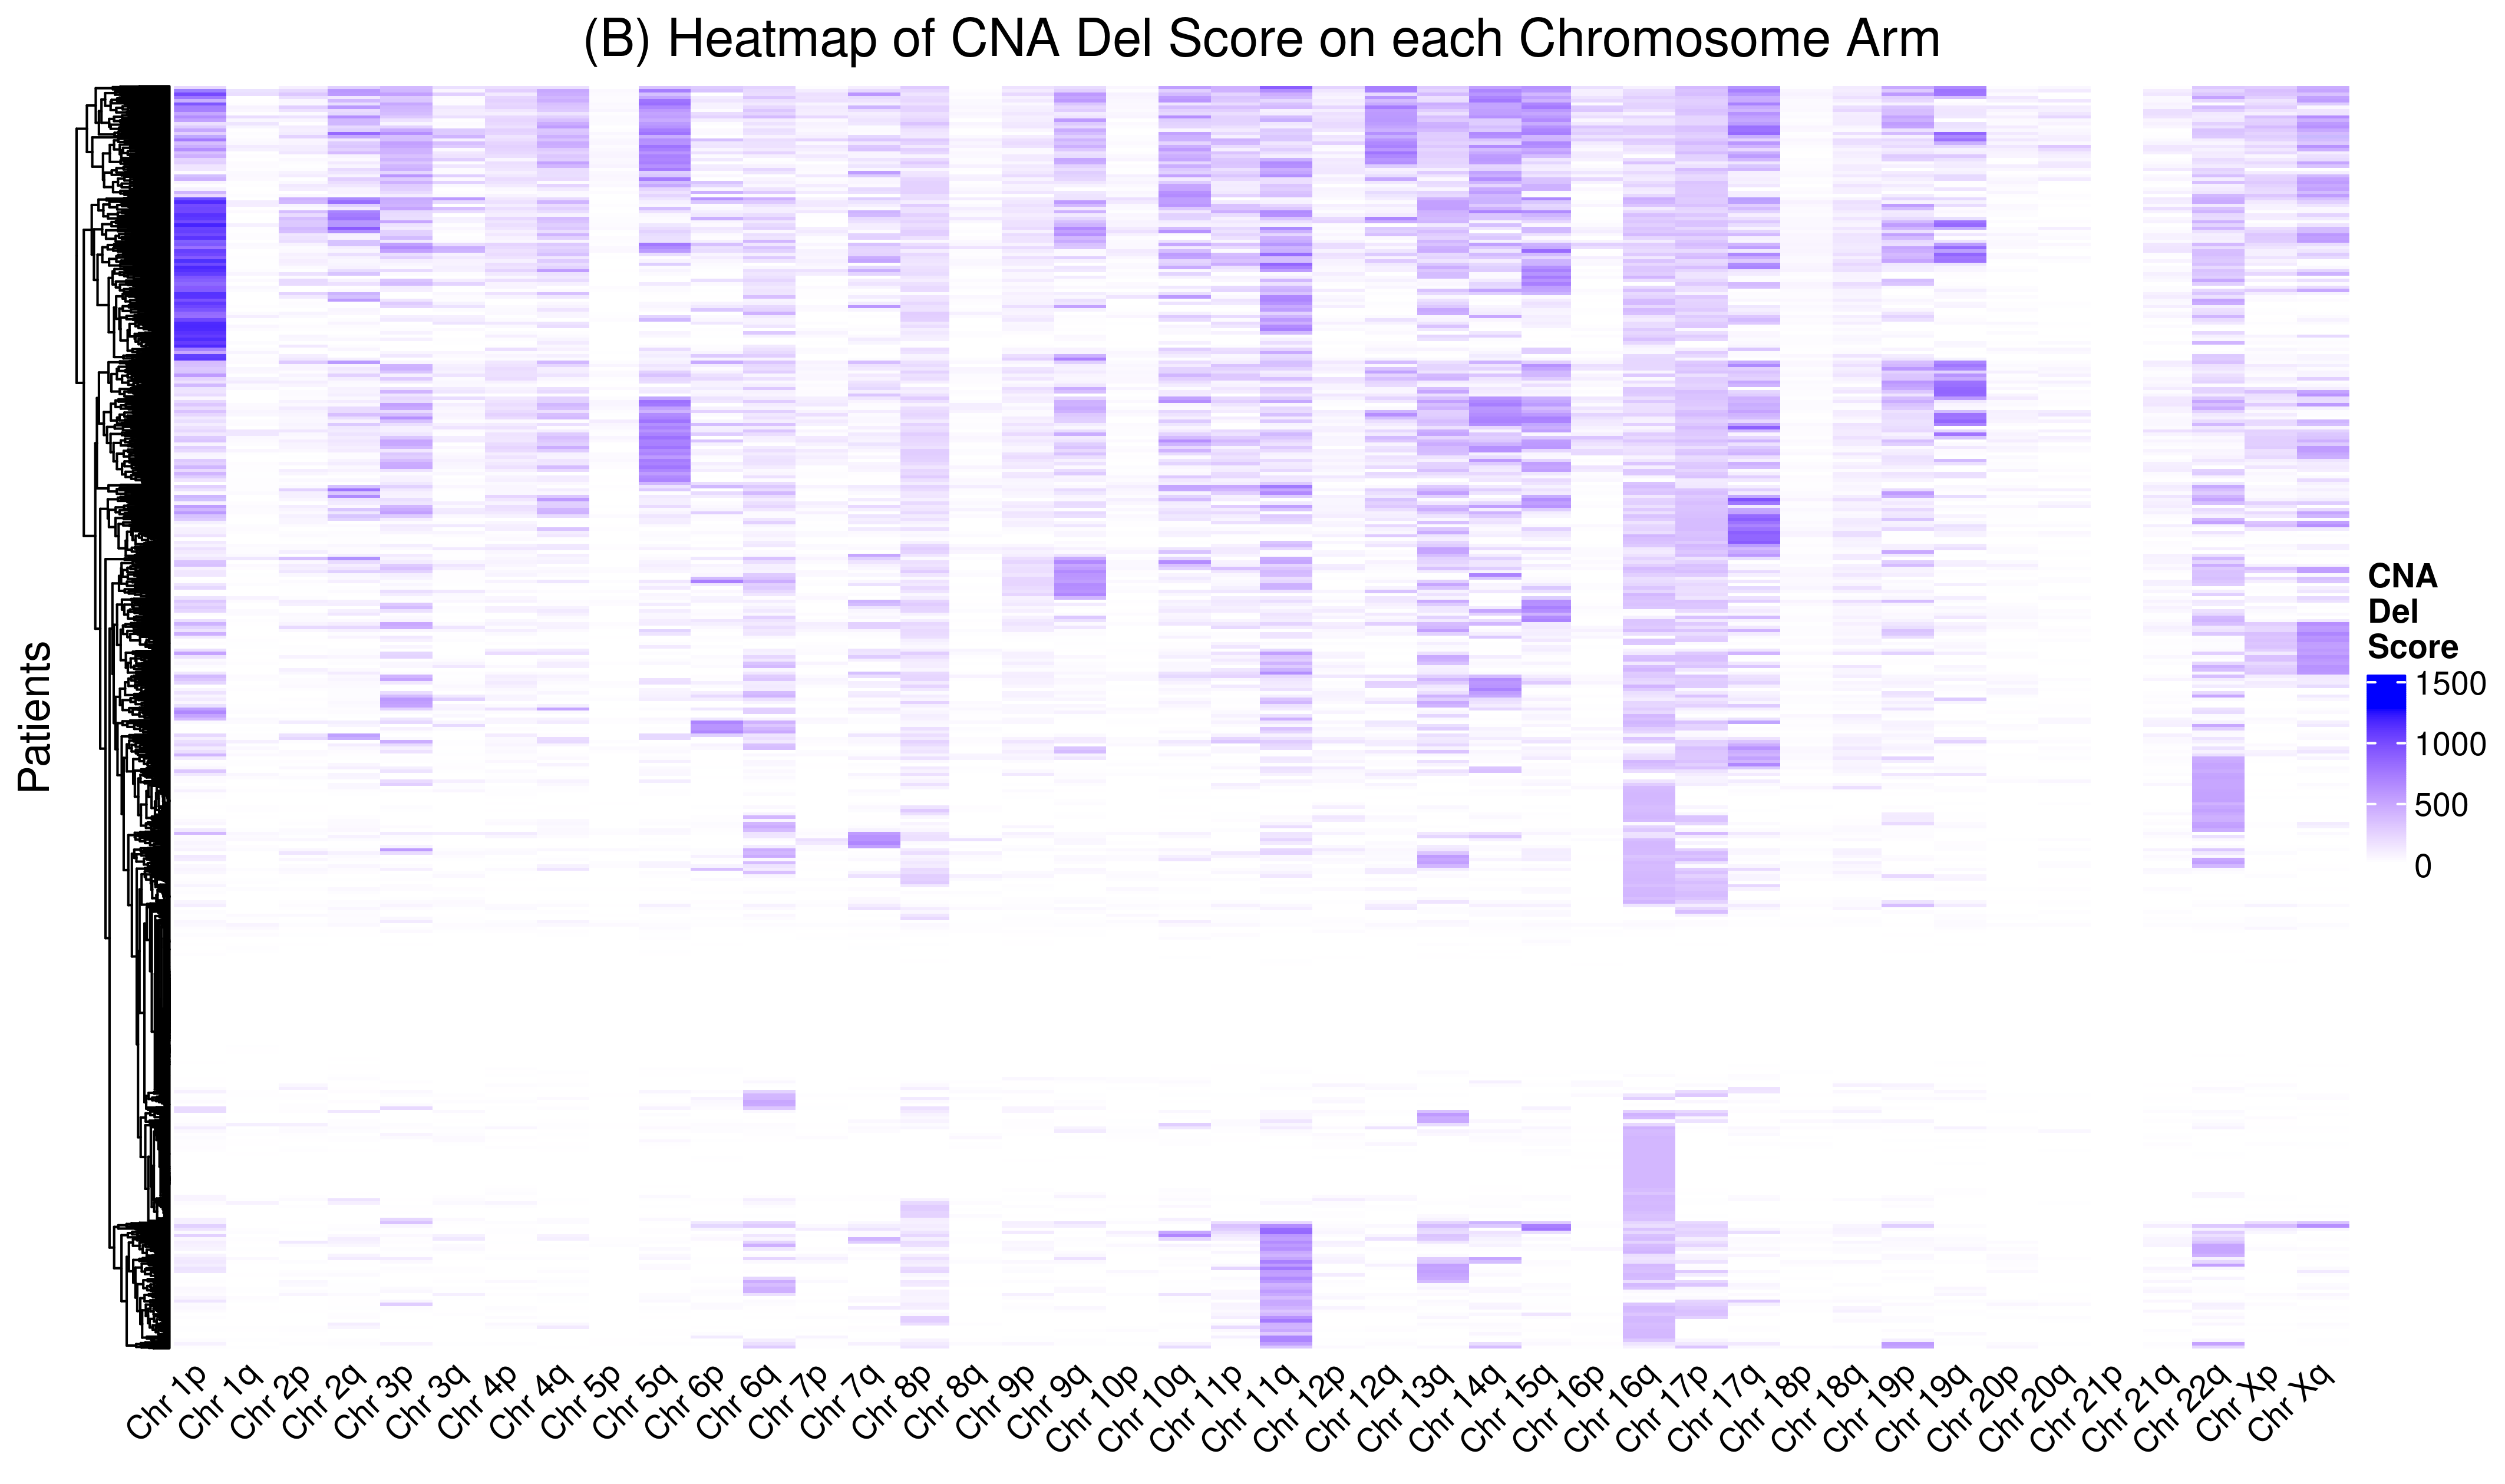
\includegraphics[width = 1.05\textwidth]{../figures/Chapter_2/CNA_Del_Score_Heatmap_All.png}
  
  \vspace{0.8cm}
  
  \caption[Heatmap of CNA Del Score across chromosome arms.]{Heatmap of CNA Del Score across chromosome arms with (A) consideration to complete-case METABRIC patients only (n = 2,091) and (B) consideration to all METABRIC patients including those presenting with some missing data (n = 2,173). Grey indicates missing values.}
  \label{SurvTrees_Score_HM}
\end{figure}
\clearpage

\begin{figure}[!ht]
  \centering
  
  \vspace{0.8cm}
  
  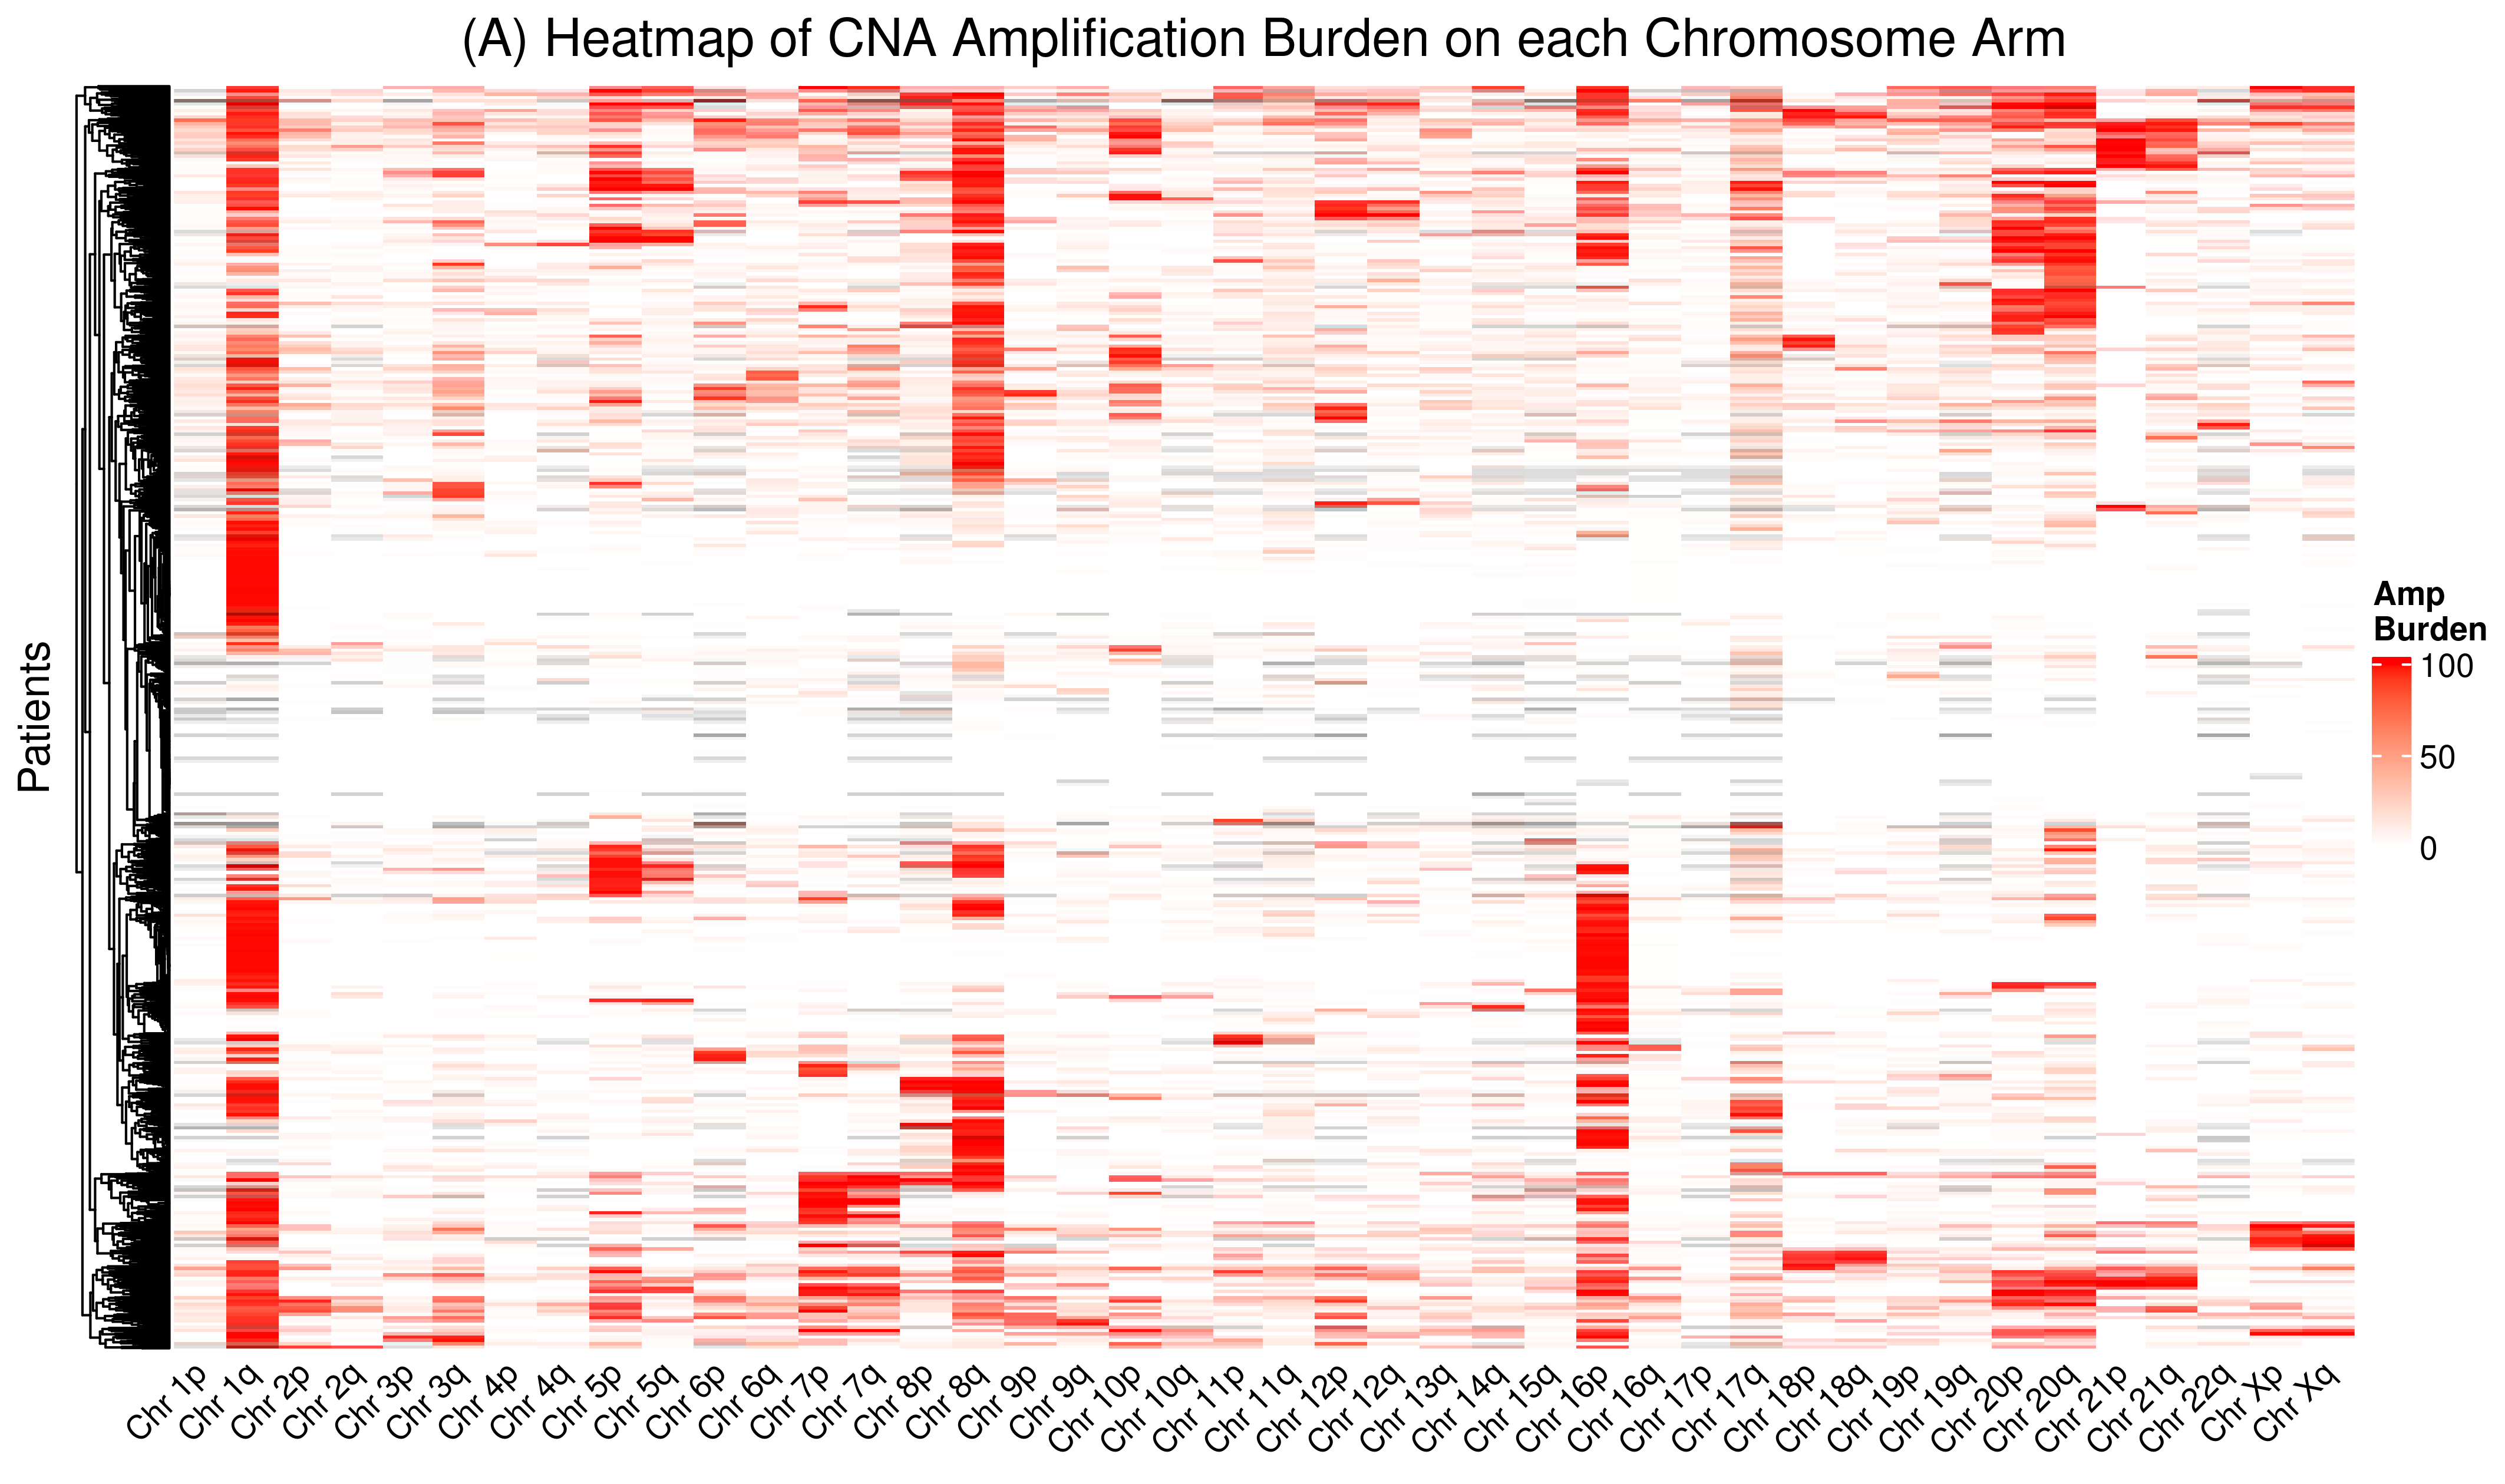
\includegraphics[width = 1.05\textwidth]{../figures/Chapter_2/CNA_Amp_Burden_Heatmap_CCA.png}
  
  \vspace{1.5cm}
  
     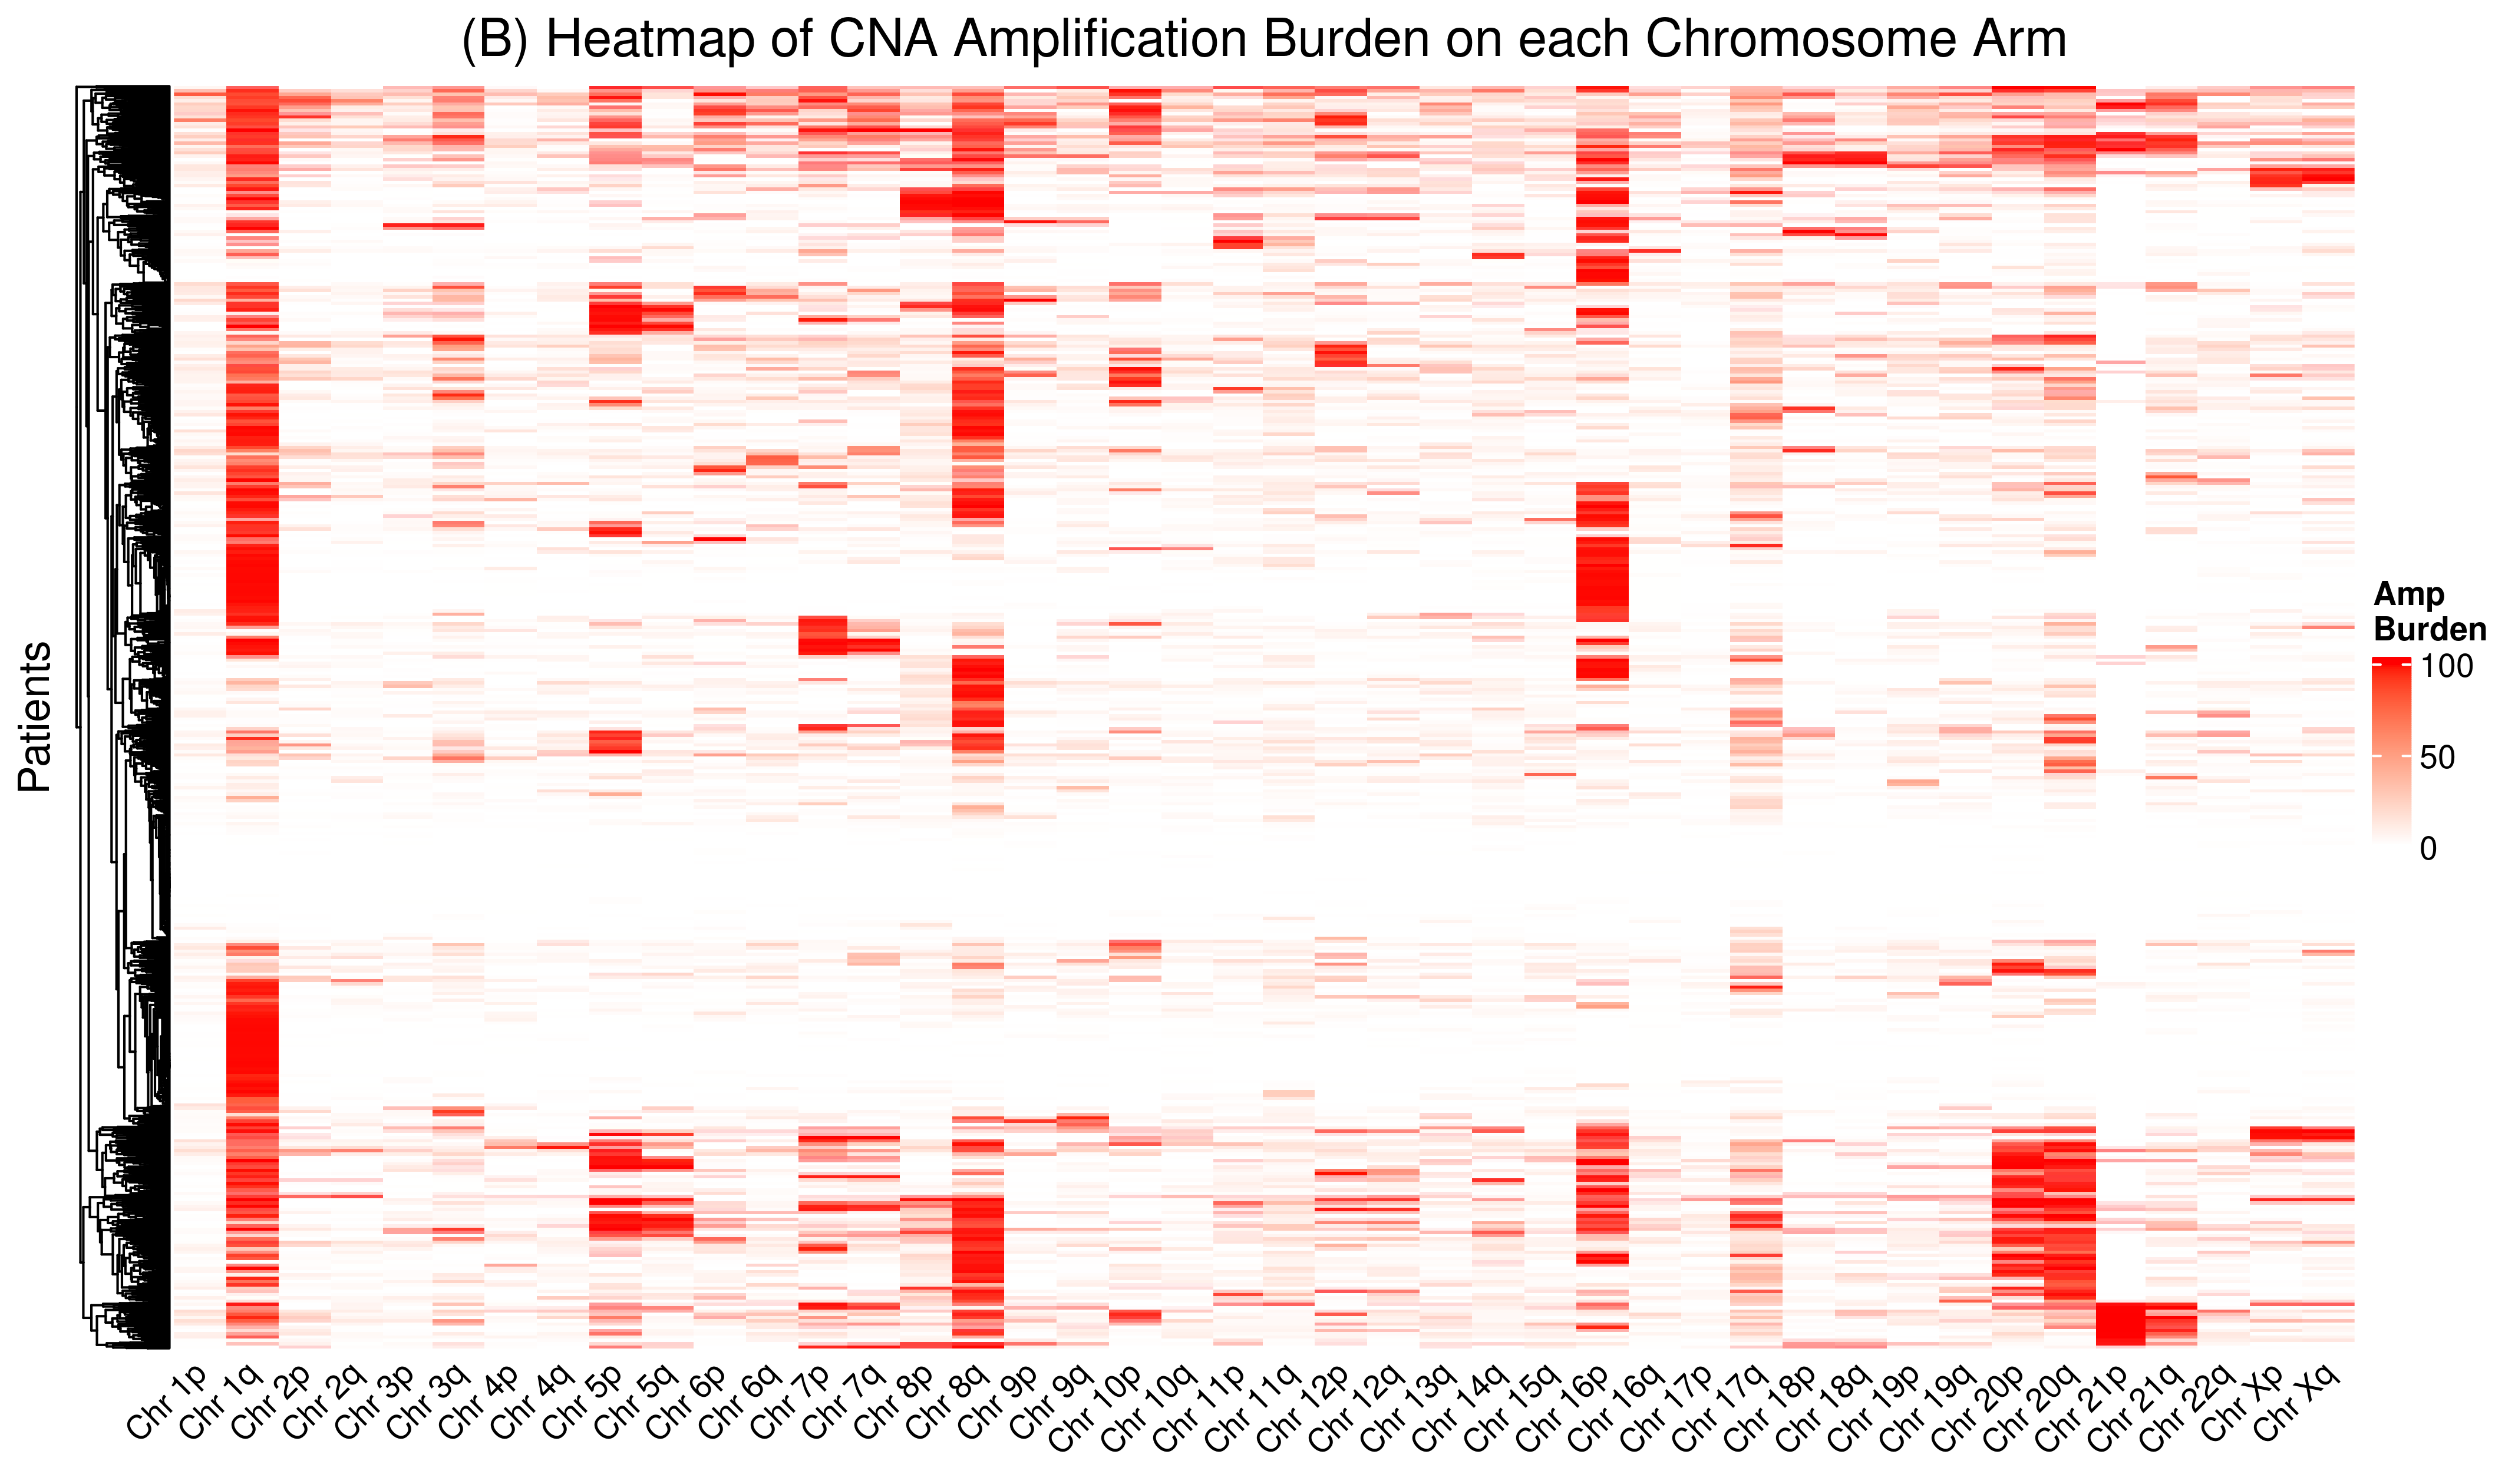
\includegraphics[width = 1.05\textwidth]{../figures/Chapter_2/CNA_Amp_Burden_Heatmap_All.png} 

\vspace{0.8cm}

  \caption[Heatmap of CNA Amp Burden across chromosome arms.]{Heatmap of CNA Amp Burden across chromosome arms with (A) consideration to complete-case METABRIC patients only (n = 2,091) and (B) consideration to all METABRIC patients including those presenting with some missing data (n = 2,173). Grey indicates missing values.}
  \label{SurvTrees_Burden_HM_CCA}
\end{figure}
\clearpage

\begin{figure}[!ht]
  \centering
  
  \vspace{0.8cm}
  
    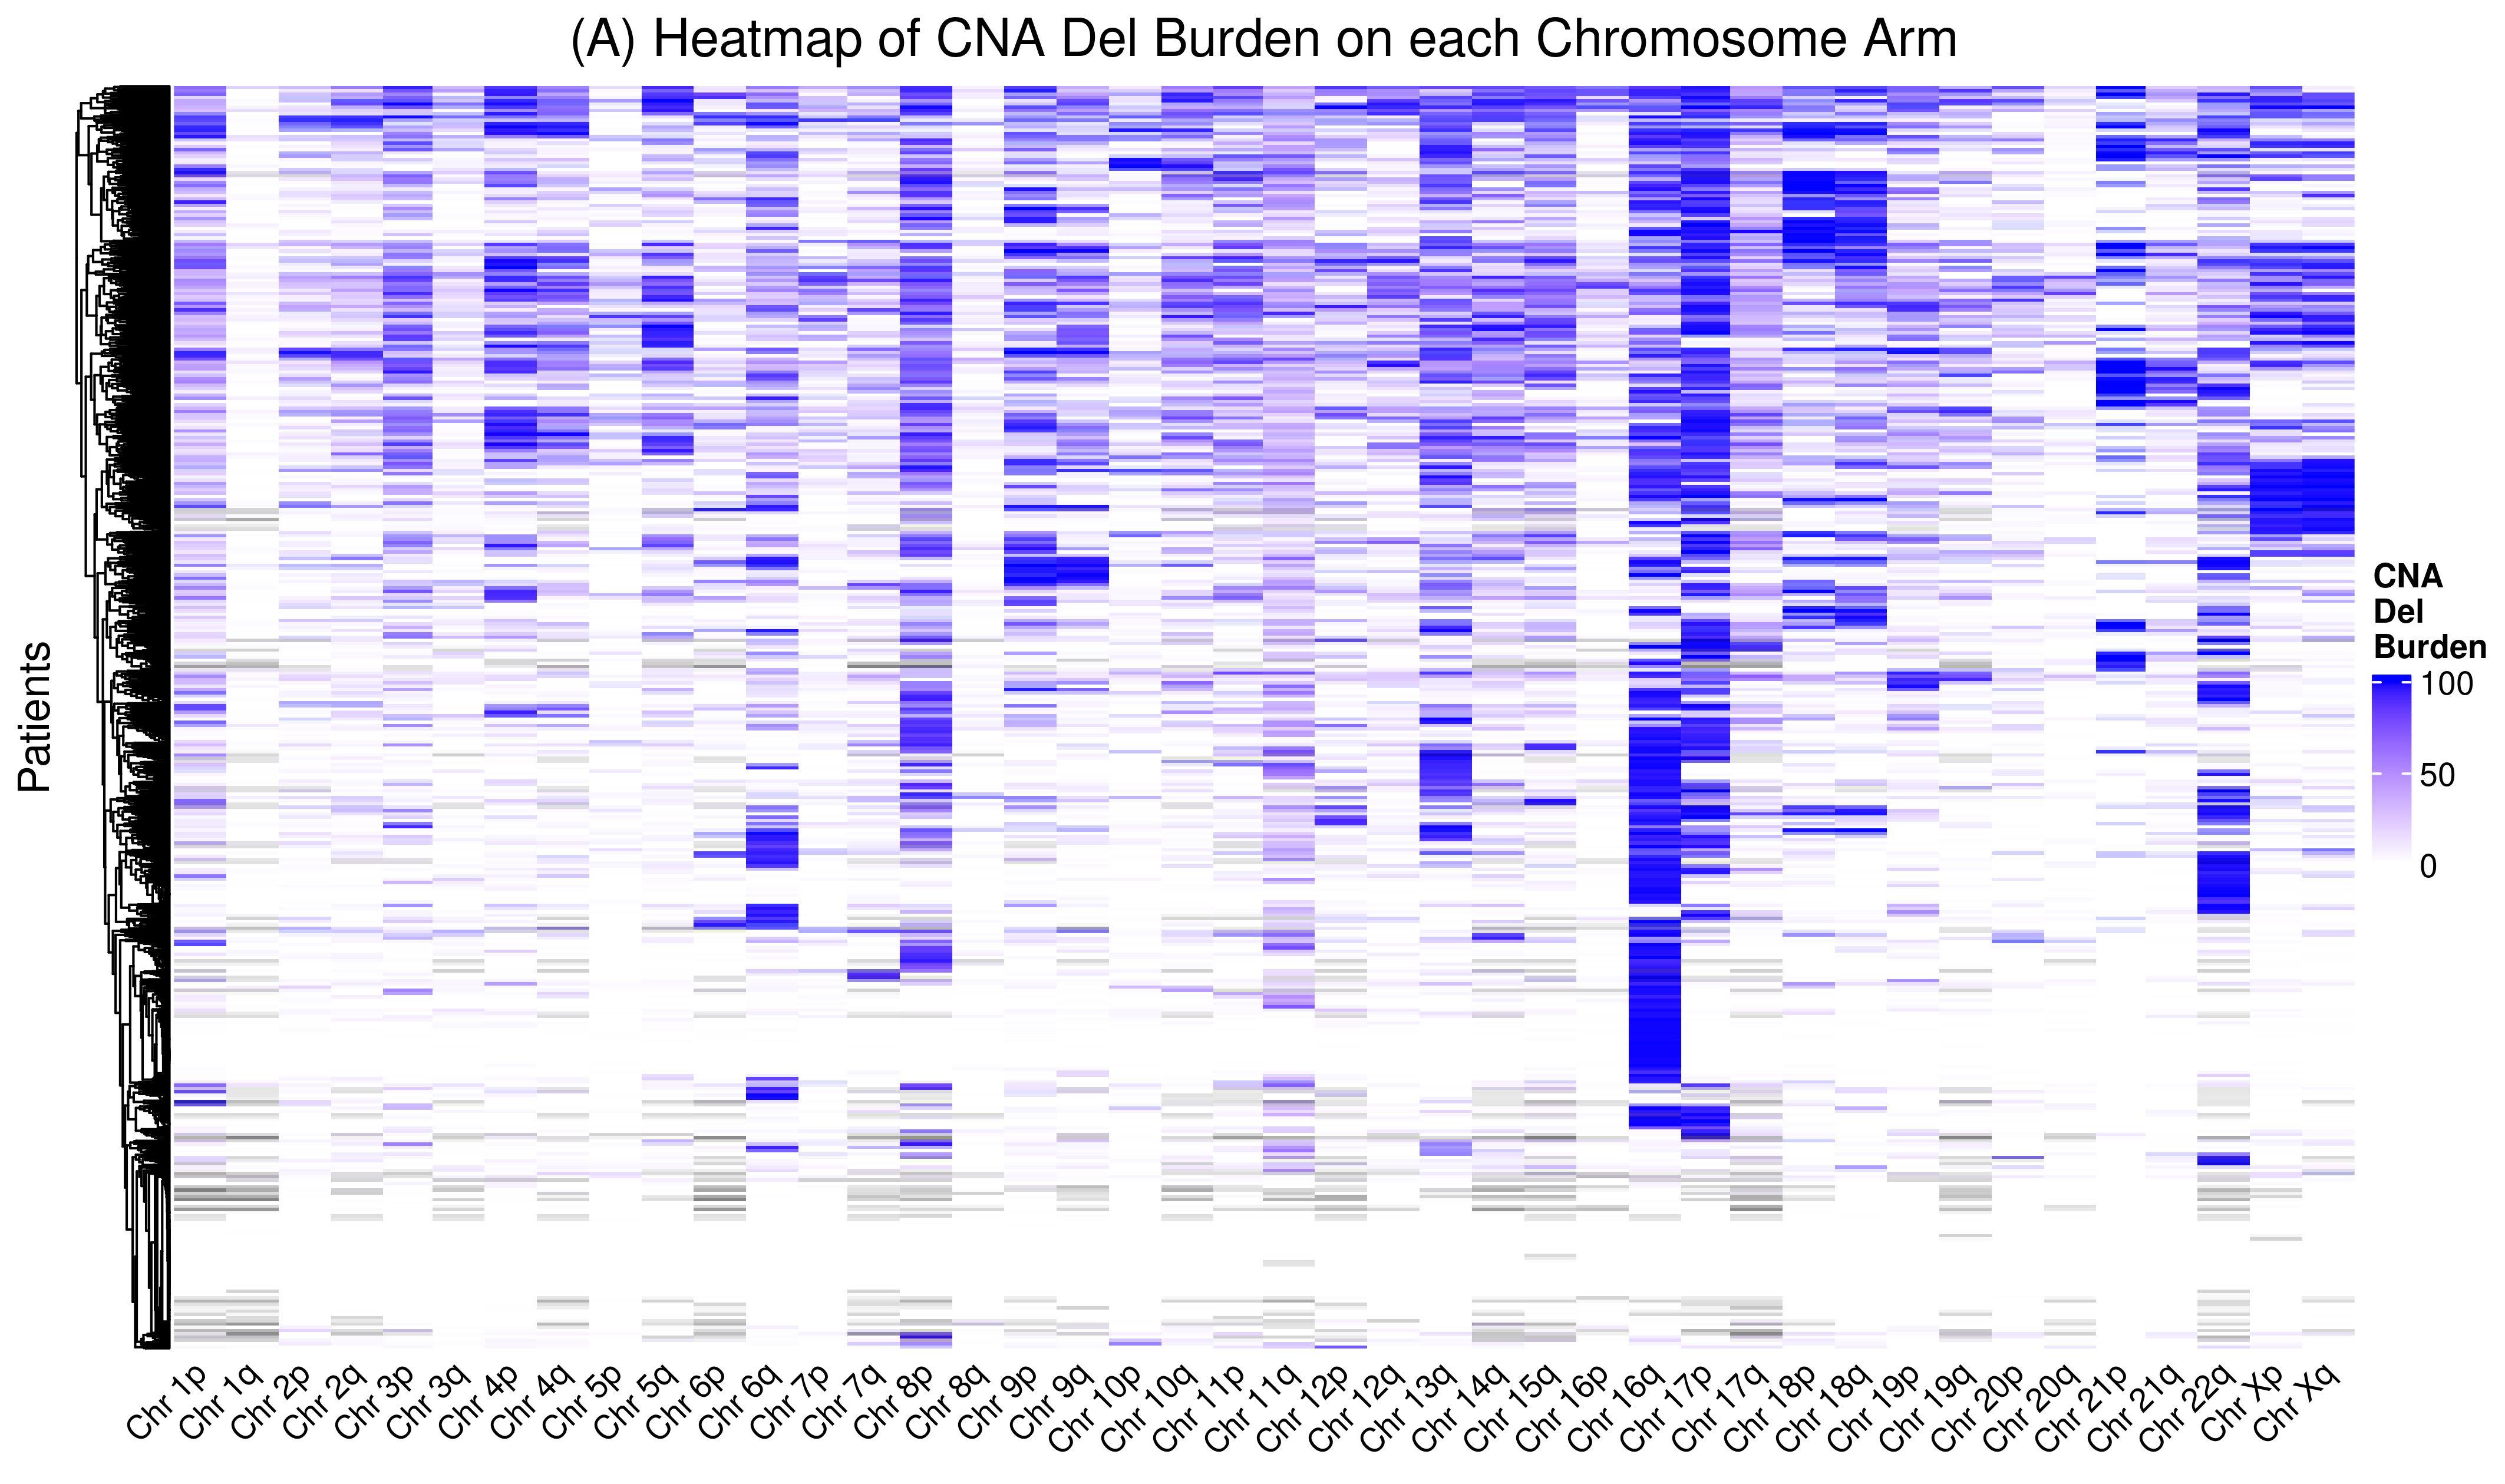
\includegraphics[width = 1.05\textwidth]{../figures/Chapter_2/CNA_Del_Burden_Heatmap_CCA.png}
    
  \vspace{1.5cm}
   
  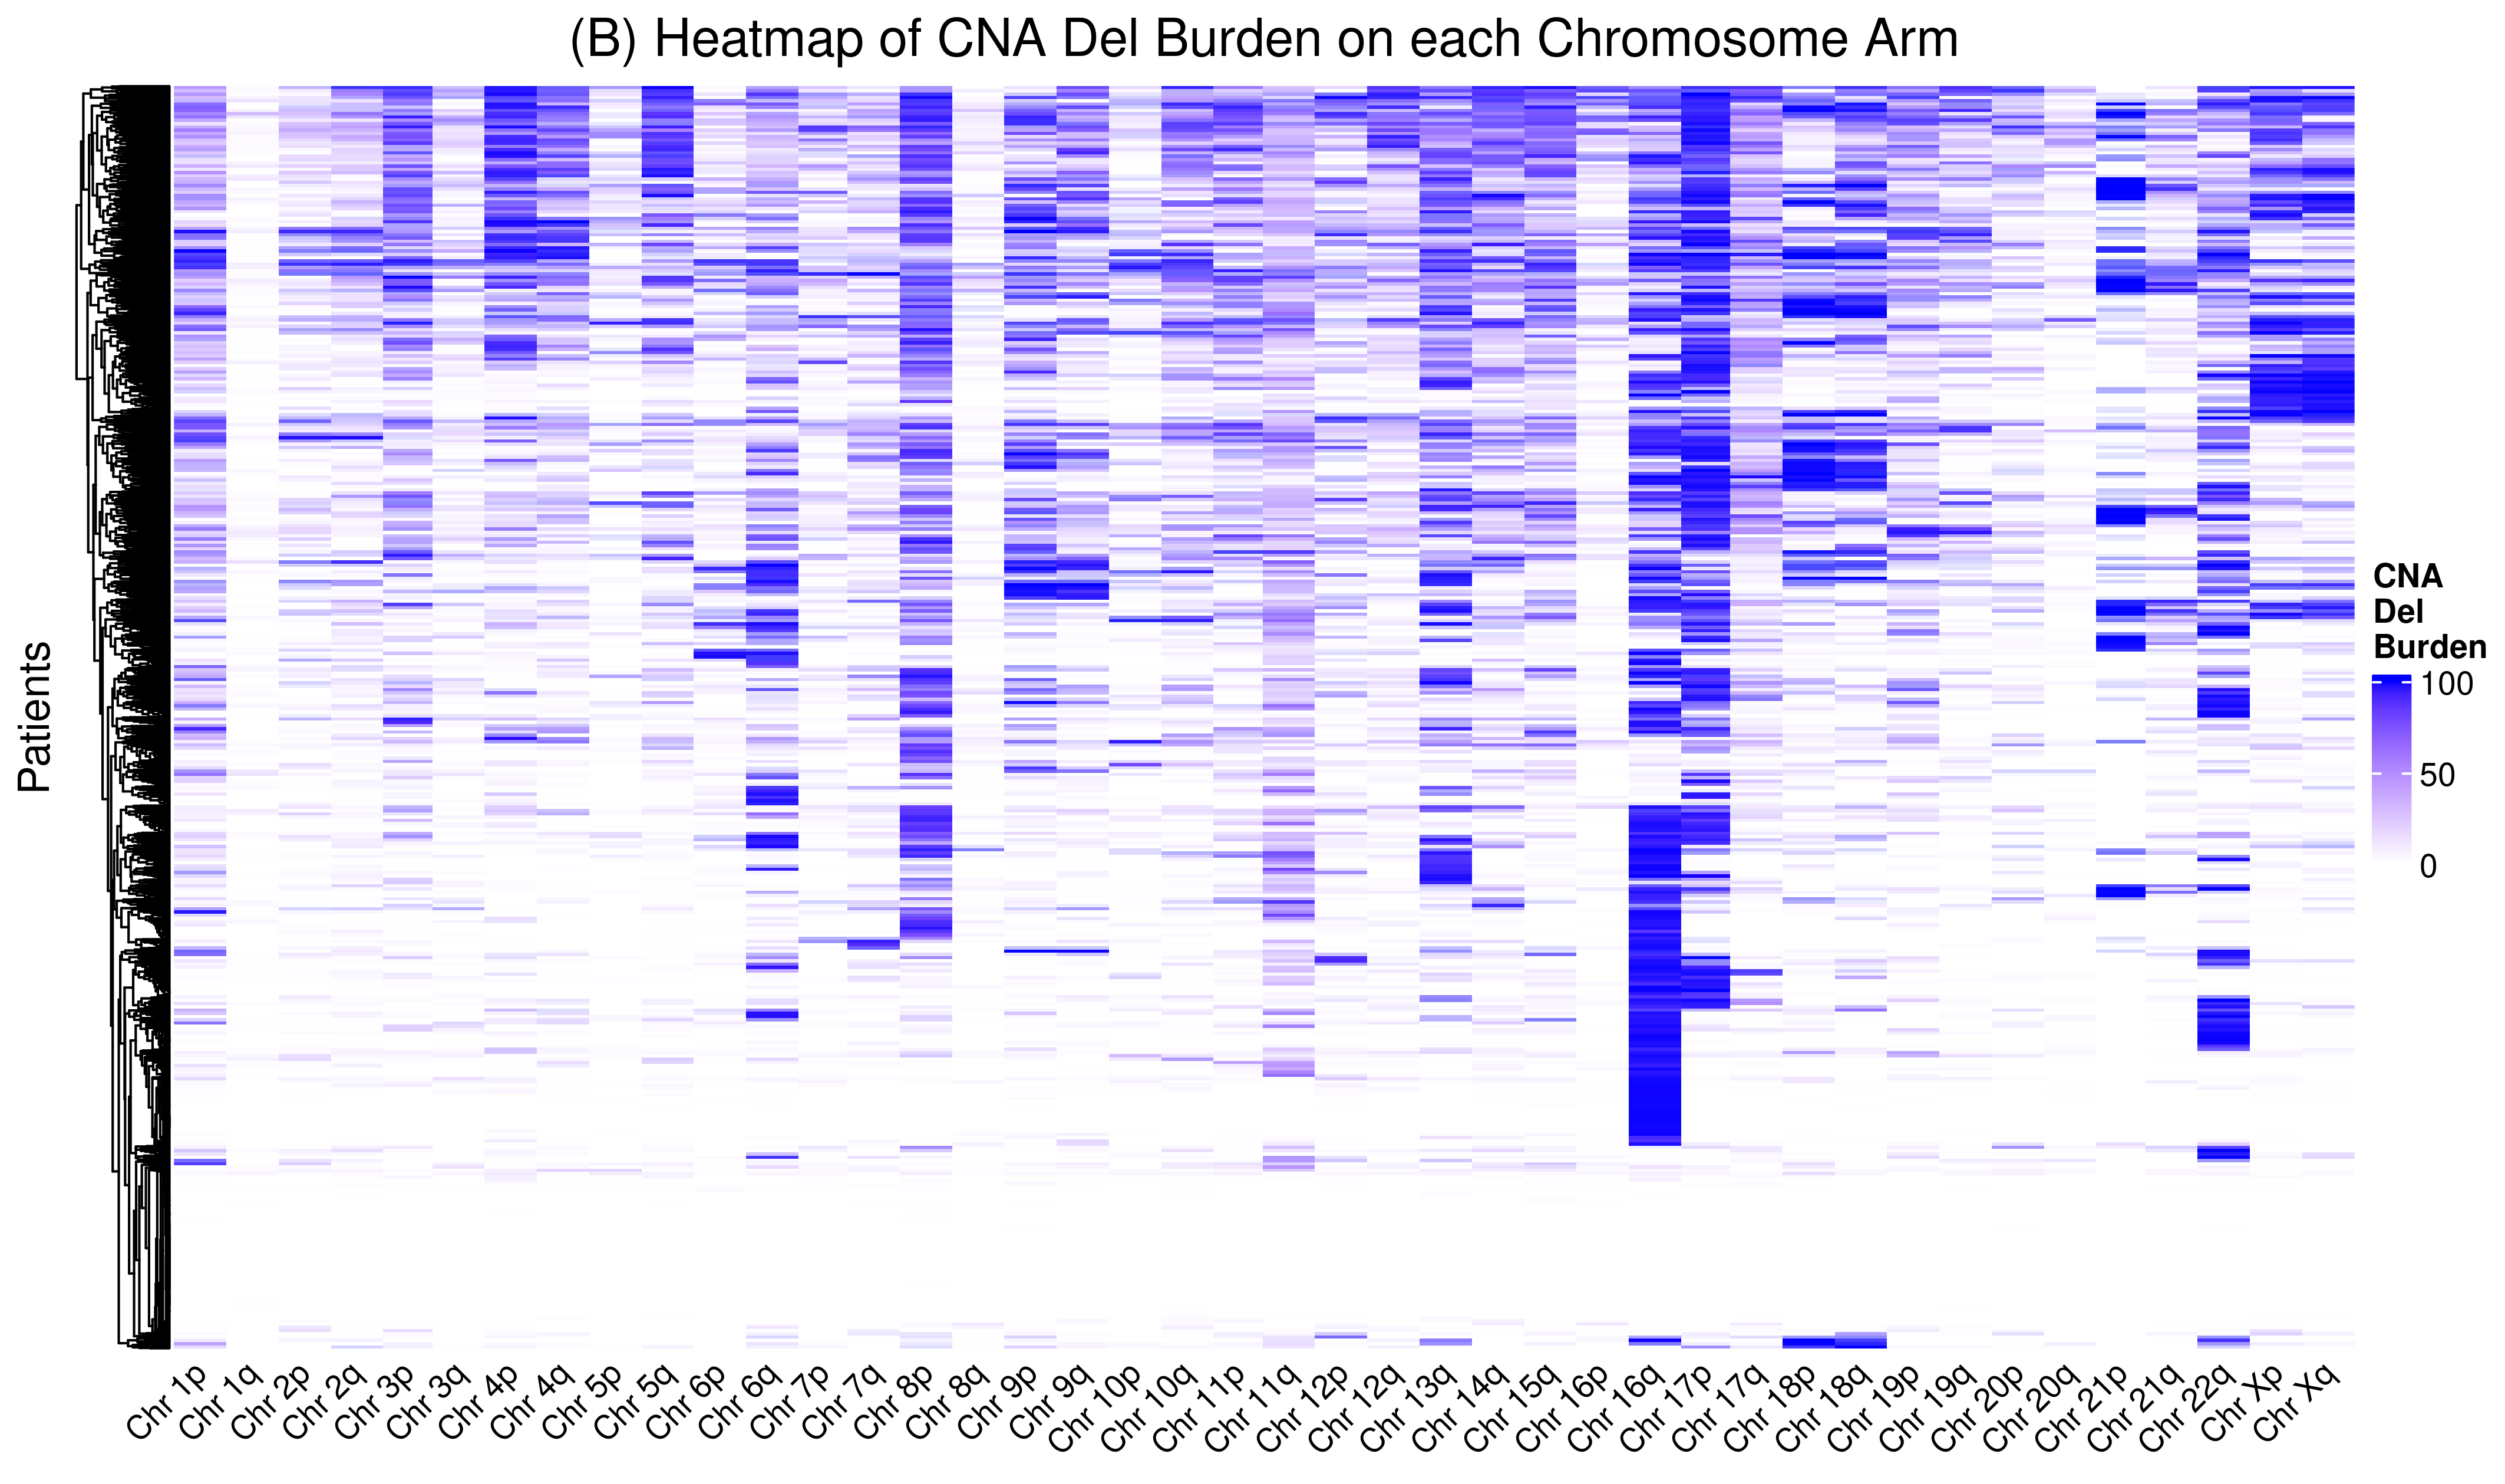
\includegraphics[width = 1.05\textwidth]{../figures/Chapter_2/CNA_Del_Burden_Heatmap_All.png}
  
  \vspace{0.8cm}
  
   \caption[Heatmap of CNA Del Burden across chromosome arms.]{Heatmap of CNA Del Burden across chromosome arms with (A) consideration to complete-case METABRIC patients only (n = 2,091) and (B) consideration to all METABRIC patients including those presenting with some missing data (n = 2,173). Grey indicates missing values.}
  \label{SurvTrees_Burden_HM}
\end{figure}

\begin{table}[!ht]
    \begin{minipage}{.49\linewidth}
      \caption[Chromosomes arms with poor overlap between complete-case patient and all-patient CNA Score metrics.]{Chromosomes arms with poor overlap between complete-case patient and all-patient CNA Score metrics. Metrics are ordered and coloured by percentage overlap.}
      \centering 
\begin{tabular}[t]{l>{}r}
\toprule
CNA Score Metric & \% Overlap\\
\midrule
\% CNA Score Amp 9p & \cellcolor[HTML]{414487}{\textcolor{white}{11.00}}\\
 
CNA Amp Score 9p & \cellcolor[HTML]{443C84}{\textcolor{white}{16.69}}\\
 
\% CNA Score Del 7p & \cellcolor[HTML]{481F70}{\textcolor{white}{42.65}}\\
 
\% CNA Score Amp 18q & \cellcolor[HTML]{481466}{\textcolor{white}{55.59}}\\
 
Difference 18p & \cellcolor[HTML]{450458}{\textcolor{white}{74.15}}\\
 
\% CNA Score Del 8q & \cellcolor[HTML]{450457}{\textcolor{white}{75.14}}\\
 
\% CNA Score Amp 22q & \cellcolor[HTML]{440256}{\textcolor{white}{76.71}}\\
 
Difference Xq & \cellcolor[HTML]{440155}{\textcolor{white}{77.85}}\\
 
Difference 18q & \cellcolor[HTML]{440155}{\textcolor{white}{78.80}}\\
 
Difference 19p & \cellcolor[HTML]{440154}{\textcolor{white}{79.10}}\\
\bottomrule
\end{tabular} \label{table:CNAScoreT2}
    \end{minipage}%
    \hspace{0.3cm}
    \begin{minipage}{.49\linewidth}
      \centering
      \caption[Chromosomes arms with poor overlap between complete-case patient and all-patient CNA Burden metrics.]{Chromosomes arms with poor overlap between complete-case patient and all-patient CNA Burden metrics. Metrics are ordered and coloured by percentage overlap.}
\begin{tabular}[t]{l>{}r}
\toprule
CNA Burden Metric & \% Overlap\\
\midrule
\% CNA Burden Amp 9p & \cellcolor[HTML]{414487}{\textcolor{white}{10.84}}\\
 
CNA Amp Burden 9p & \cellcolor[HTML]{443B84}{\textcolor{white}{16.83}}\\
 
\% CNA Burden Del 7p & \cellcolor[HTML]{481C6E}{\textcolor{white}{45.26}}\\
 
\% CNA Burden Amp 18q & \cellcolor[HTML]{460B5E}{\textcolor{white}{65.25}}\\
 
CNA Amp Burden Xq & \cellcolor[HTML]{46075B}{\textcolor{white}{67.35}}\\
 
Difference 19p & \cellcolor[HTML]{46065A}{\textcolor{white}{70.39}}\\
 
\% CNA Burden Amp 22q & \cellcolor[HTML]{450457}{\textcolor{white}{72.01}}\\
 
Difference 18p & \cellcolor[HTML]{450357}{\textcolor{white}{76.29}}\\
 
Difference Xq & \cellcolor[HTML]{440154}{\textcolor{white}{77.29}}\\
 
Difference 18q & \cellcolor[HTML]{440154}{\textcolor{white}{79.68}}\\
\bottomrule
\end{tabular} \label{table:CNABurdenT2}
    \end{minipage}
\end{table}

\vfill
\begin{figure}[H]
\vspace{0.1cm}
\begin{minipage}{.49\textwidth}
    \subfloat[]{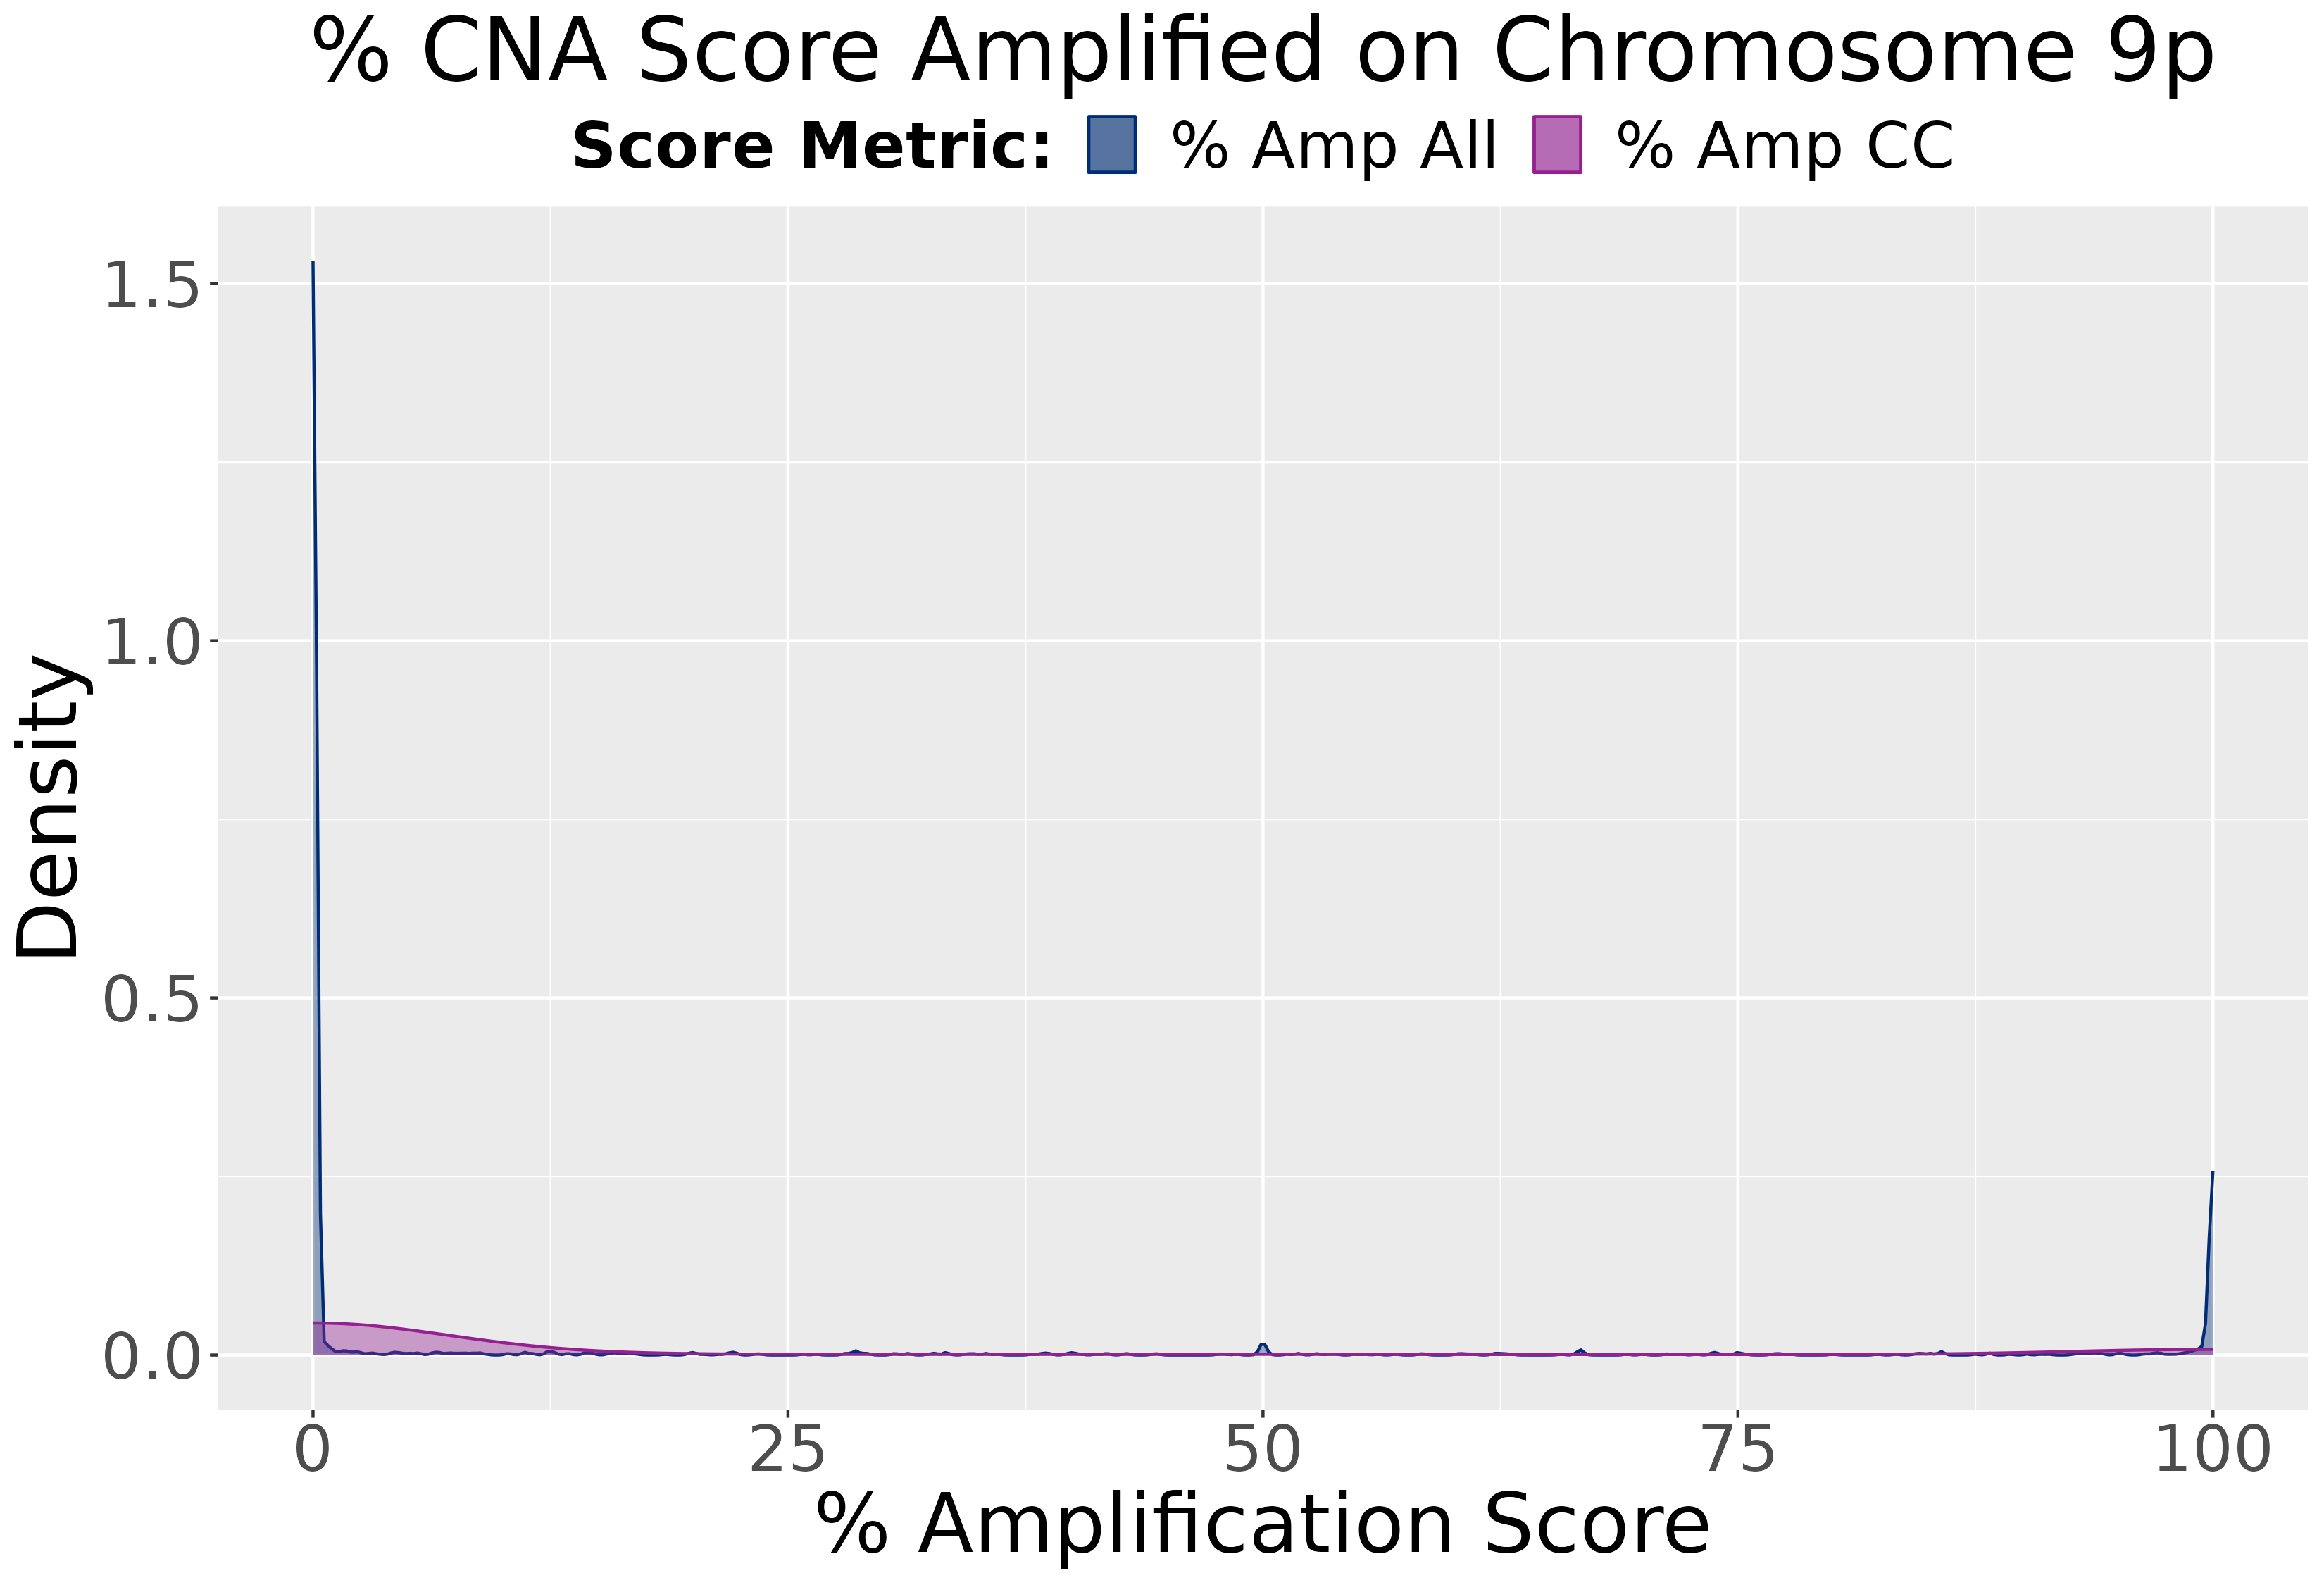
\includegraphics[width=\textwidth]{../figures/Chapter_2/CNA_Score_9p.png}}
\end{minipage}
\hfill   
\begin{minipage}{.49\textwidth}
    \subfloat[]{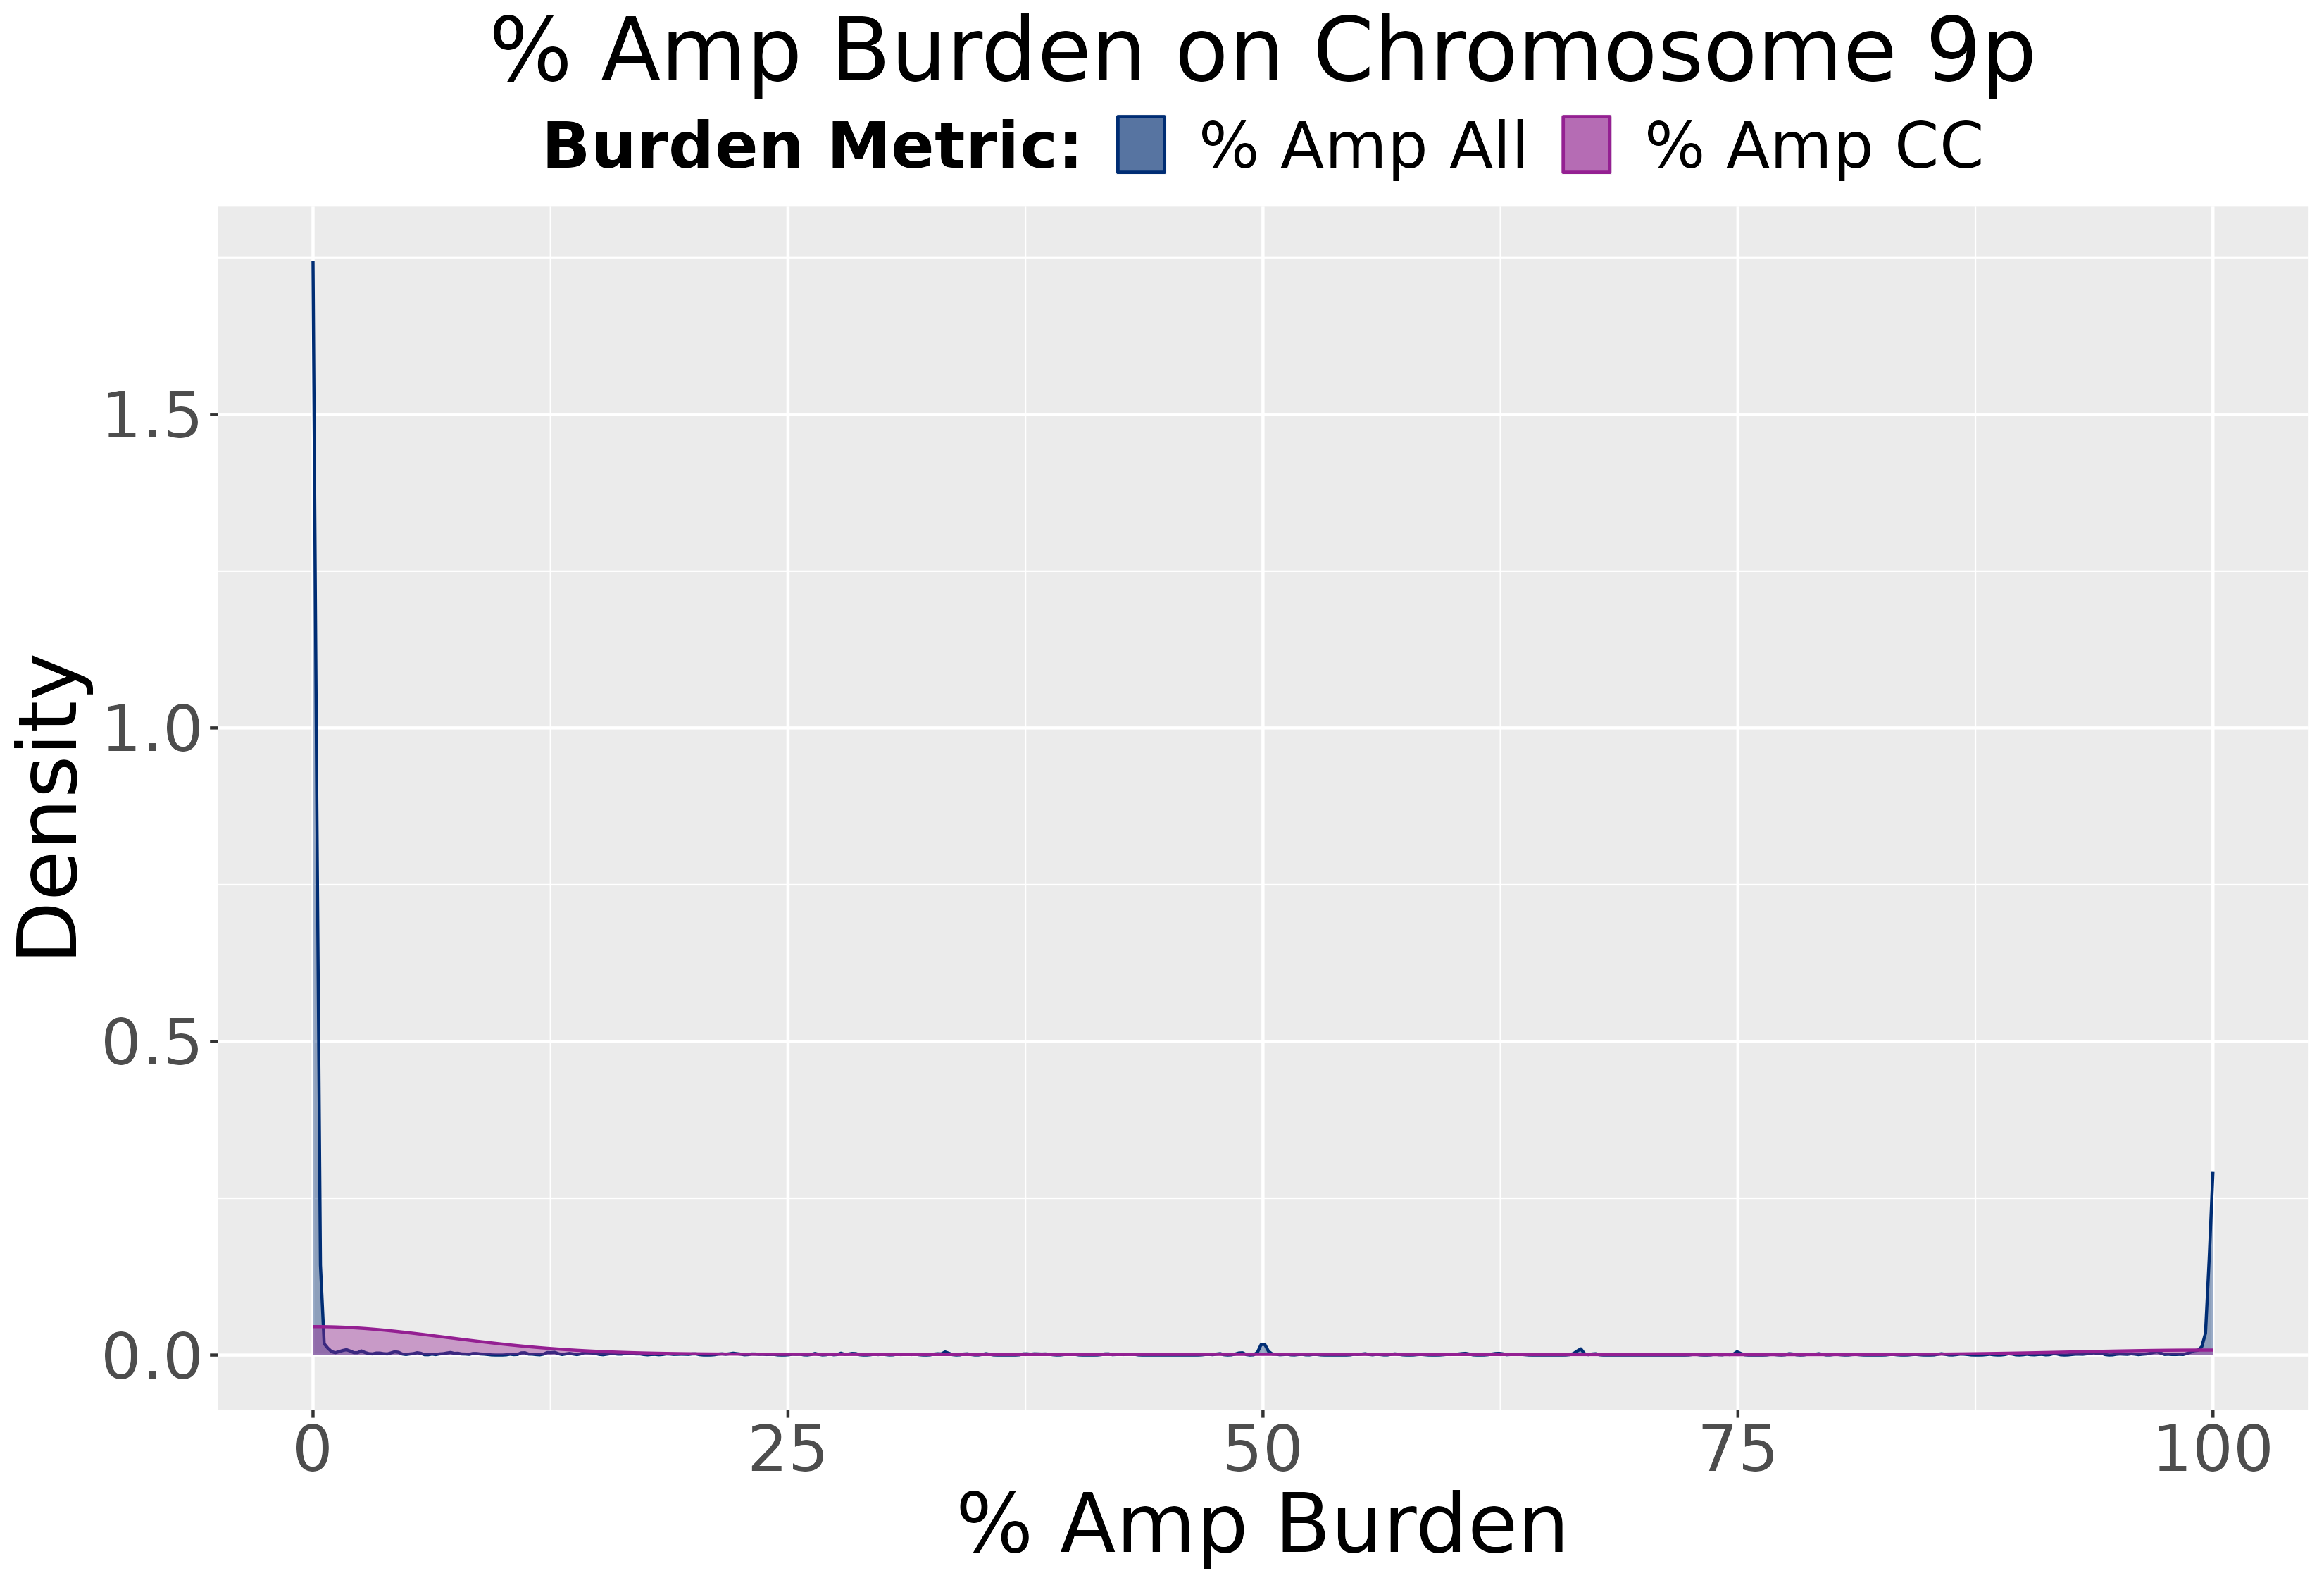
\includegraphics[width=\textwidth]{../figures/Chapter_2/CNA_Burden_9p.png}}
\end{minipage}
\hfill
\begin{minipage}{.49\textwidth}
    \subfloat[]{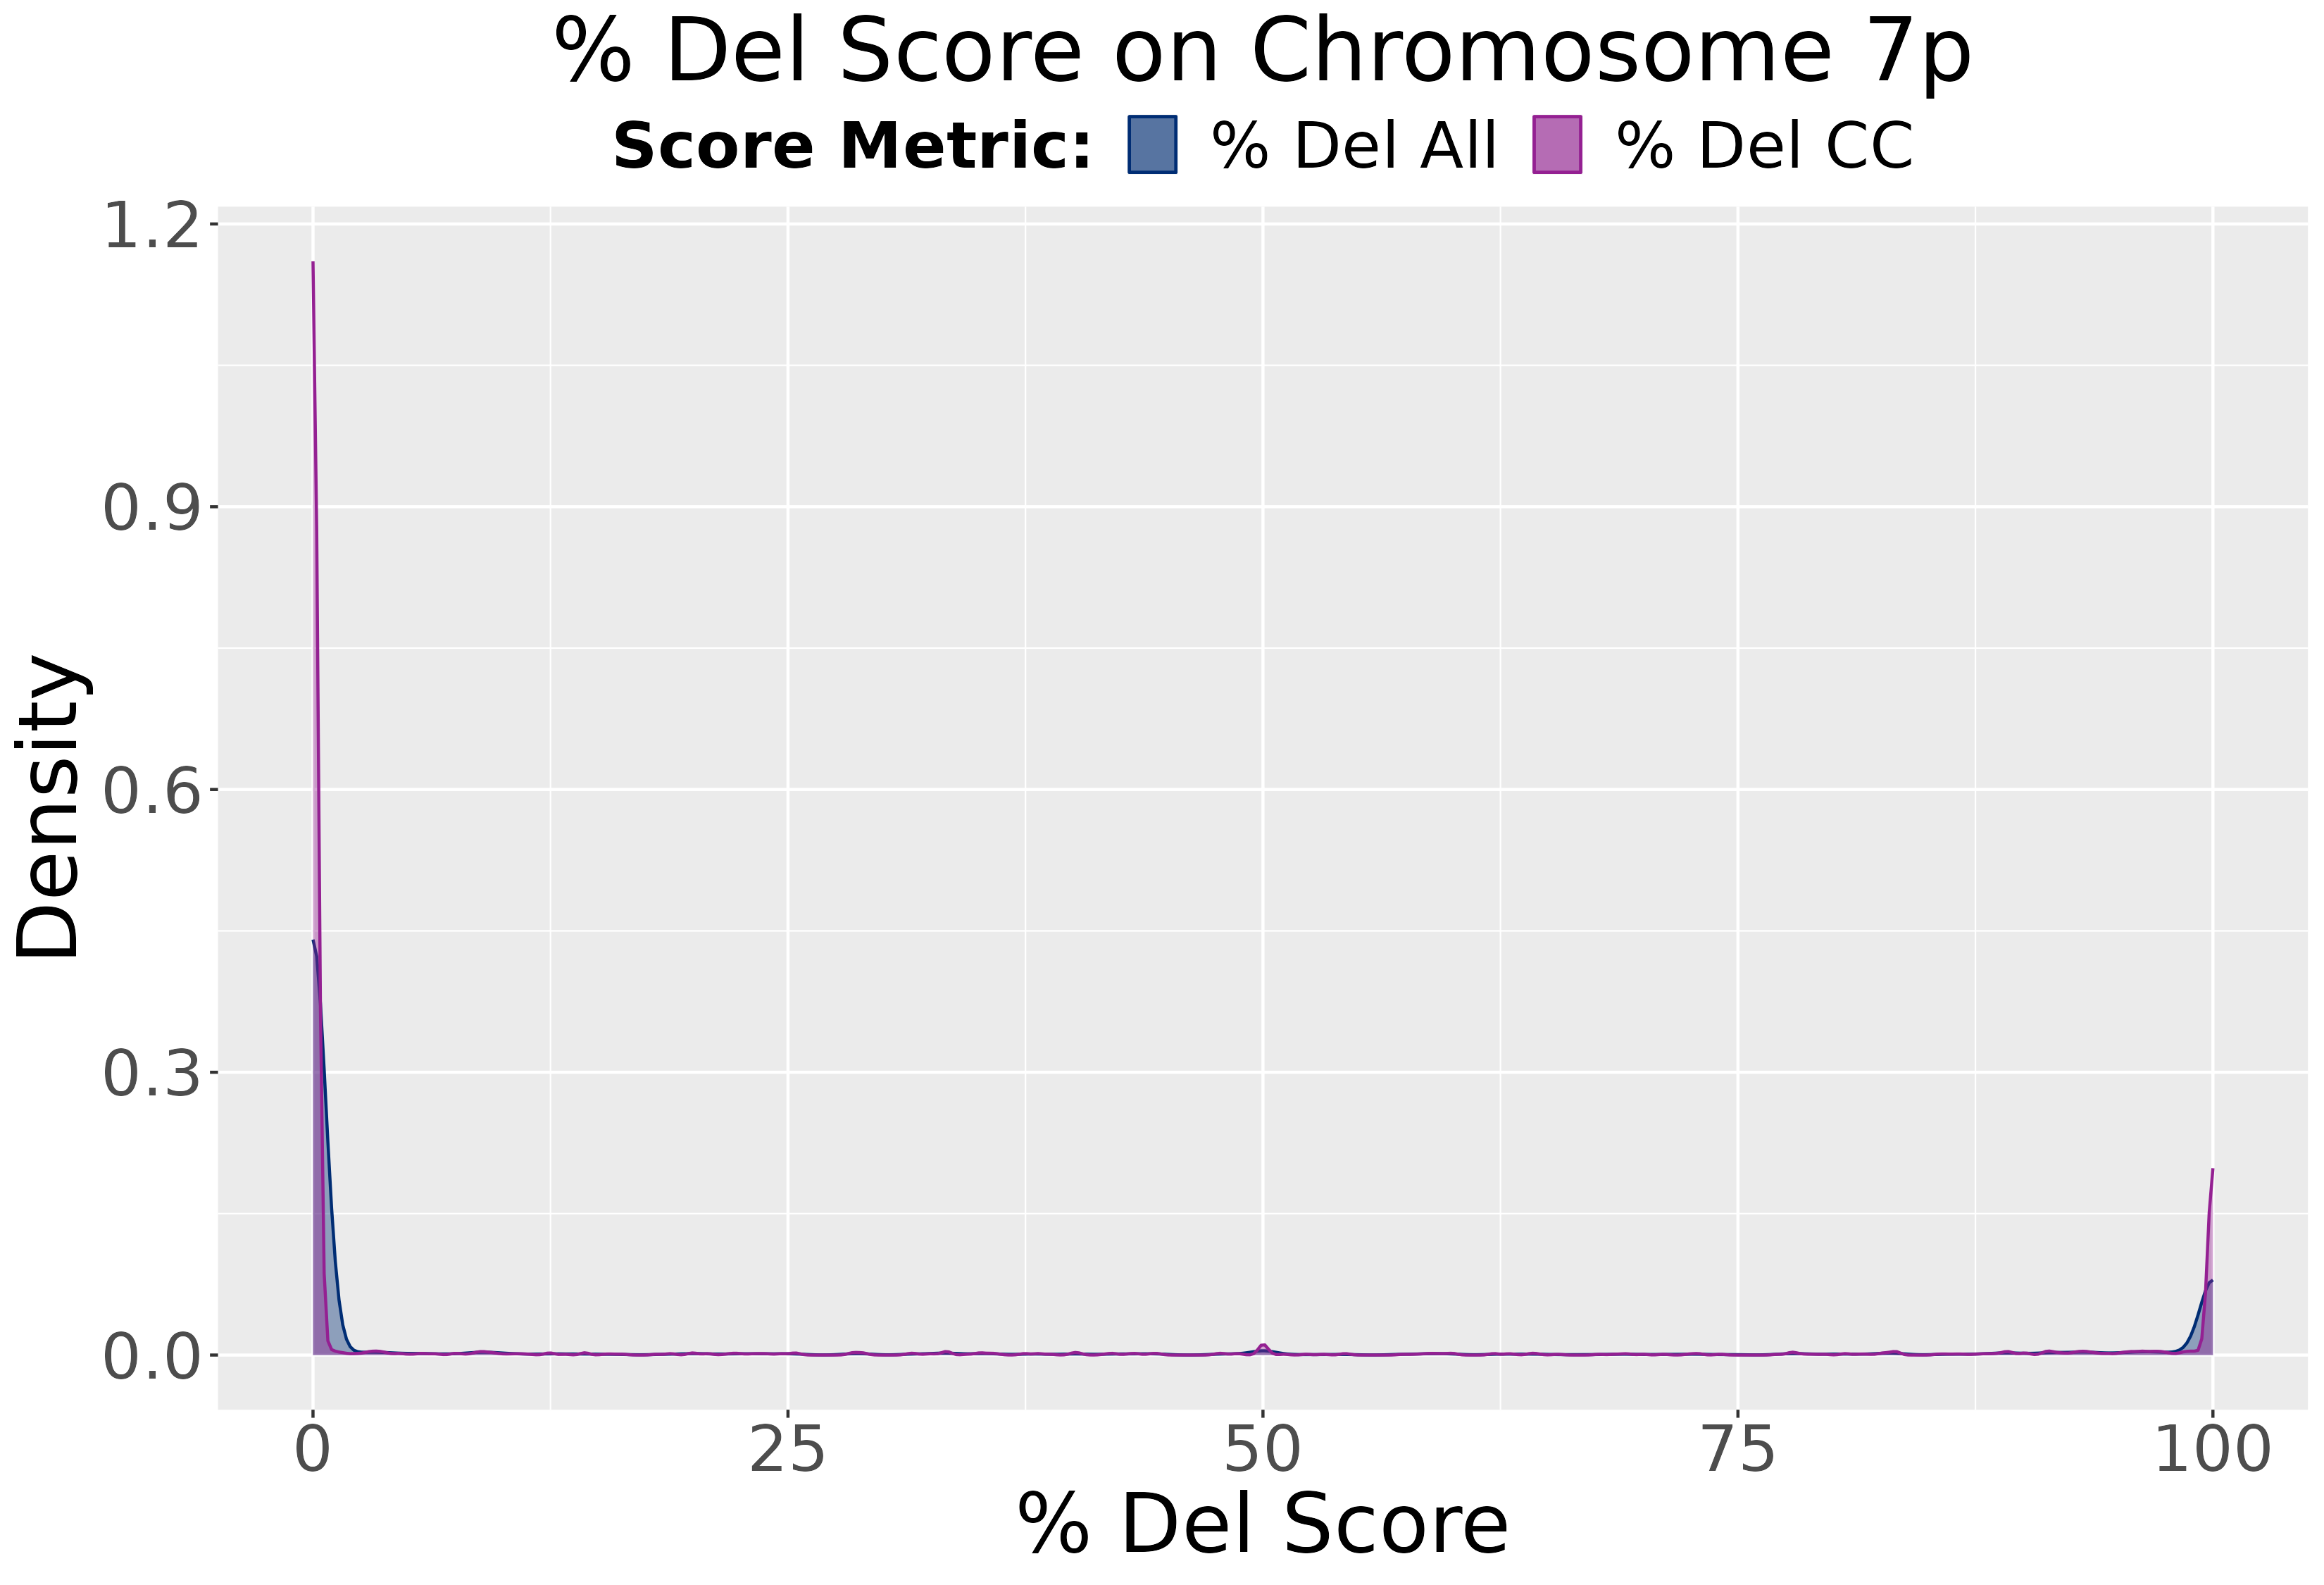
\includegraphics[width=\textwidth]{../figures/Chapter_2/CNA_Score_7p.png}}
\end{minipage}
\hfill    
\begin{minipage}{.49\textwidth}
    \subfloat[]{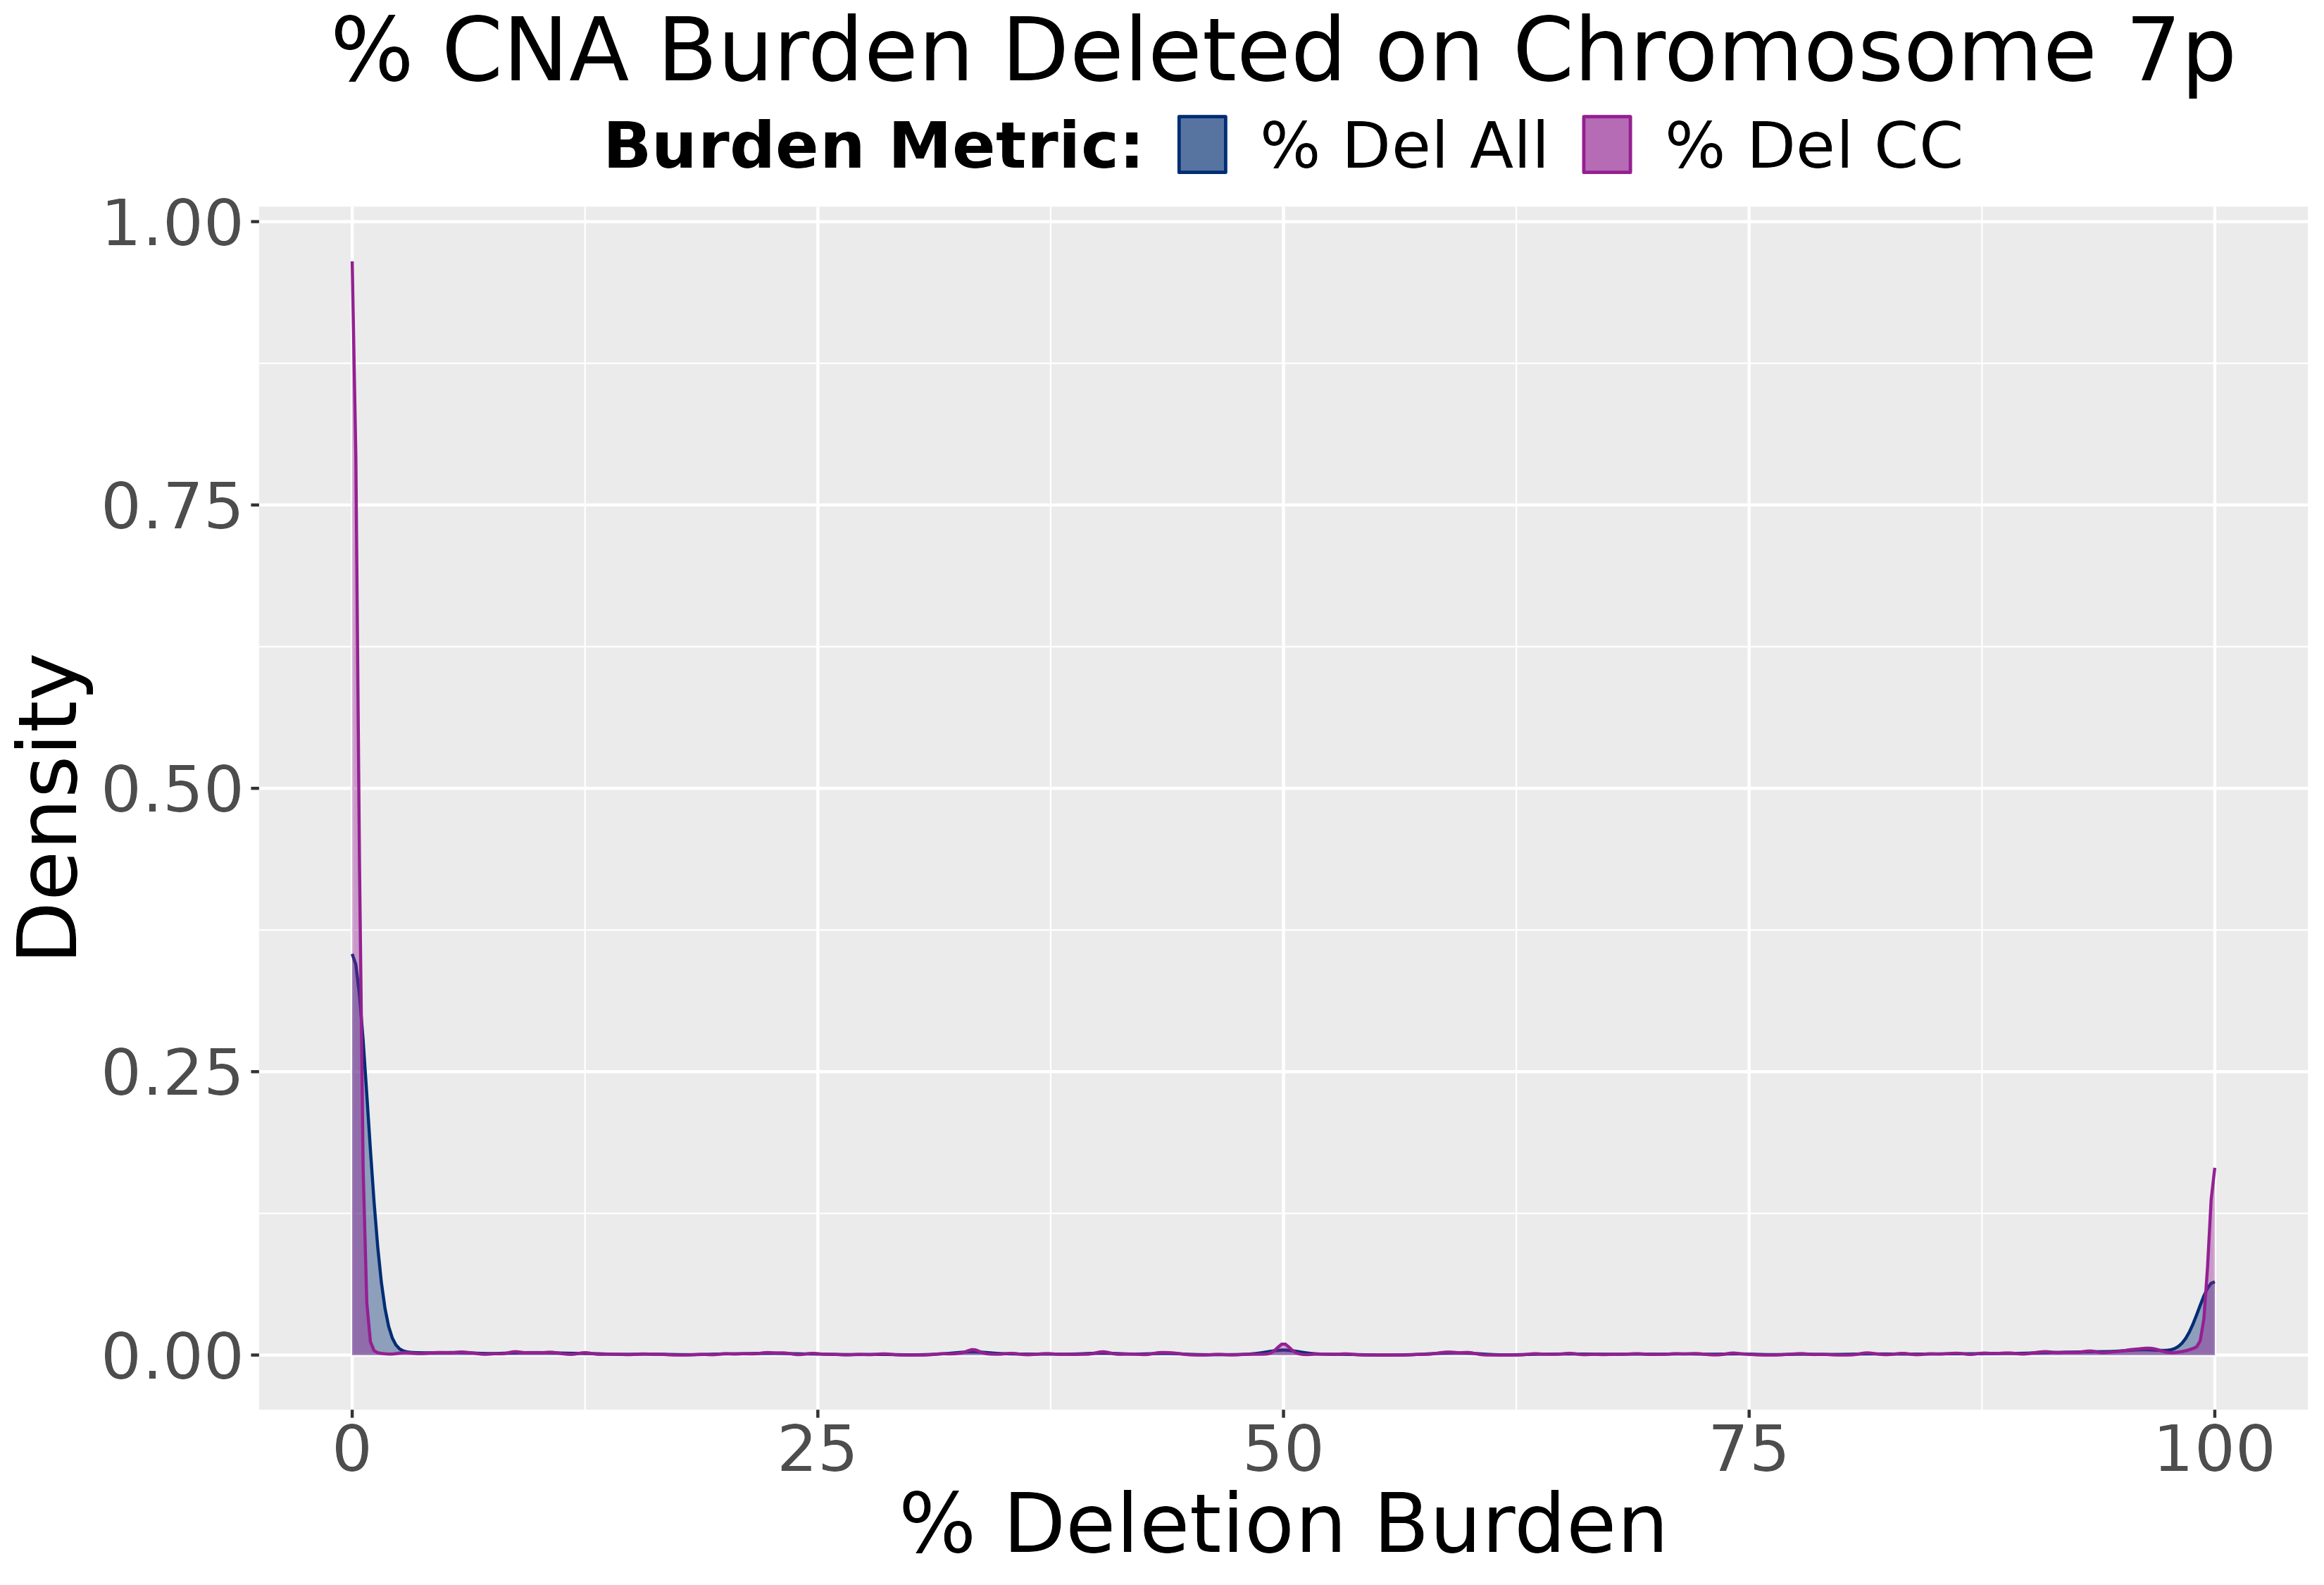
\includegraphics[width=\textwidth]{../figures/Chapter_2/CNA_Burden_7p.png}}
\end{minipage}
    \caption[Density plots for selected chromosome arm CNA metrics.]{Density plots for selected chromosome arm CNA metrics. (A) Percentage CNA Score Amp on chromosome 9p, (B) Percentage CNA Burden Amp on chromosome 9p, (C) Percentage CNA Score Del on chromosome 7p and (D) Percentage CNA Burden Del on chromosome 7p. Each plot contains density plots for both the complete-case metric and the metric calculated using all available data.}\label{fig:Plot-PerArm-DensityPlots}
\end{figure} 
\vfill 

\begin{table}[!ht]
\center
\caption[Summary statistics of the CNA Score metrics on chromosome 1q where all available data is used.]{Summary statistics of the CNA Score metrics on chromosome 1q  where all available data is used.}
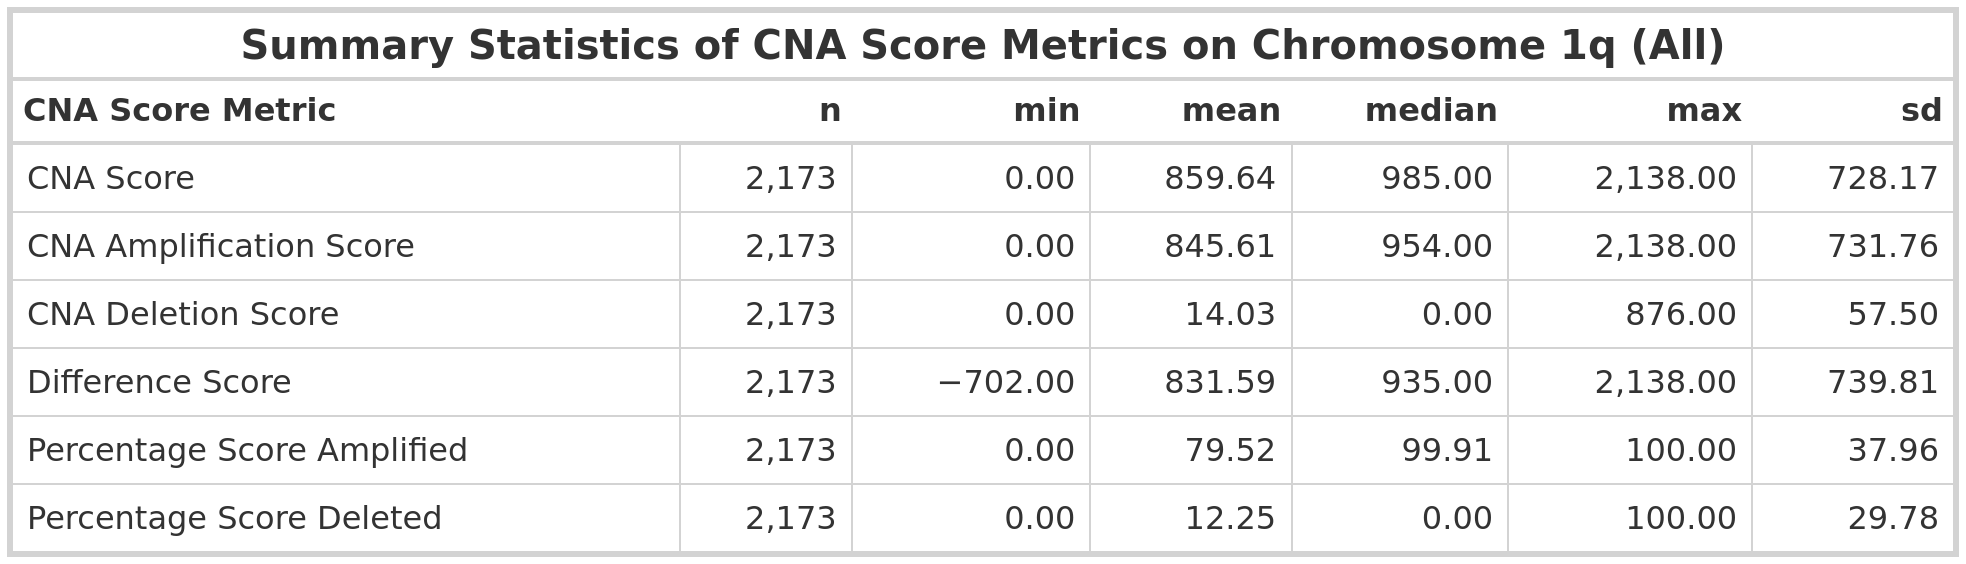
\includegraphics[width = 0.98\textwidth]{../tables/Chapter_2/CNA_Score_Metric_All_Chr1q_Summary.png}
\label{tab:Score_All_Chr1q}
\end{table}

\begin{table}[!ht]
\center
\caption[Summary statistics of the CNA Score metrics on chromosome 1q where only complete cases are used.]{Summary statistics of the CNA Score metrics on chromosome 1q where only complete cases are used.}
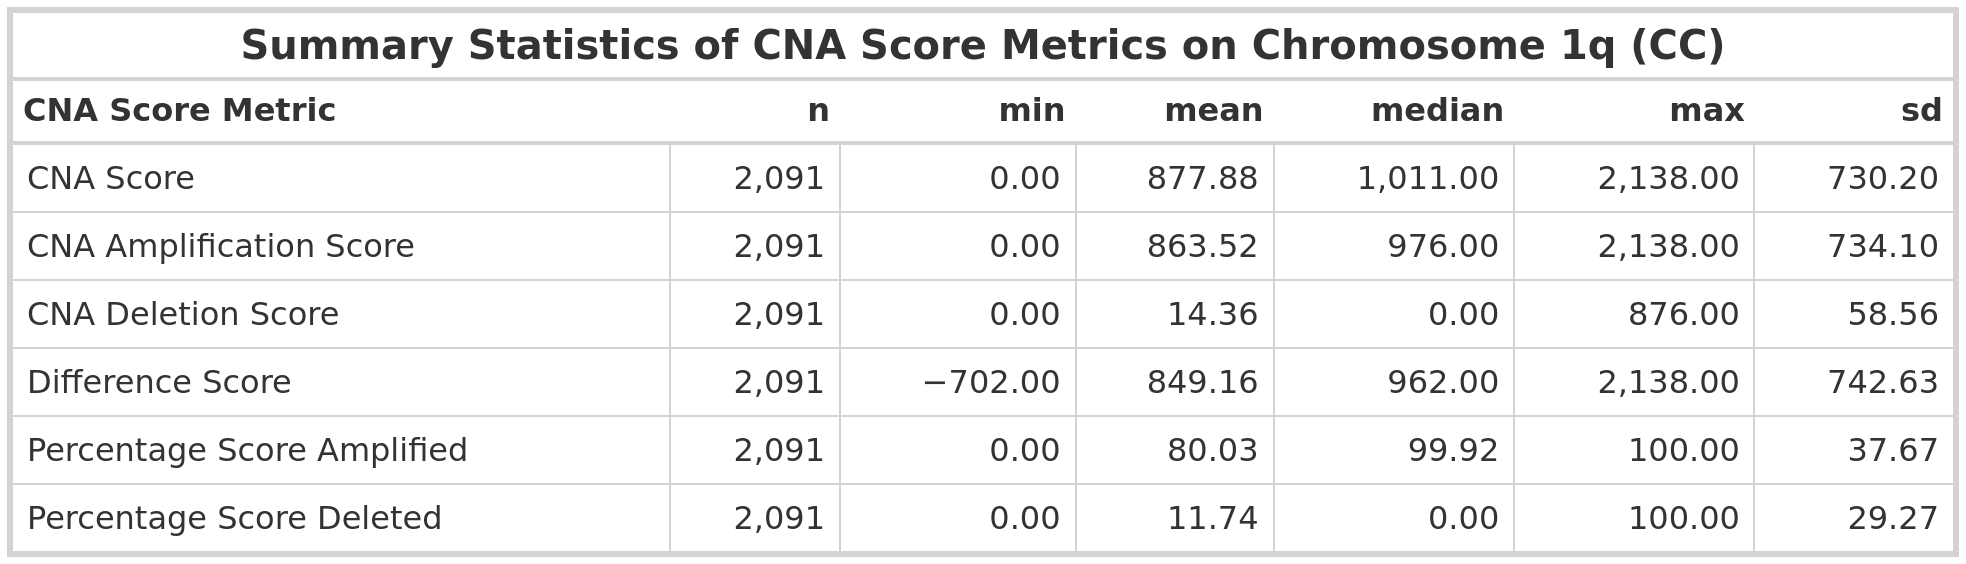
\includegraphics[width = 0.98\textwidth]{../tables/Chapter_2/CNA_Score_Metric_CCA_Chr1q_Summary.png}
\label{tab:Score_CCA_Chr1q}
\end{table}

\begin{table}[!ht]
\center
\caption[Summary statistics of the CNA Burden metrics on chromosome 1q where all available data is used.]{Summary statistics of the CNA Burden metrics on chromosome 1q where all available data is used.}
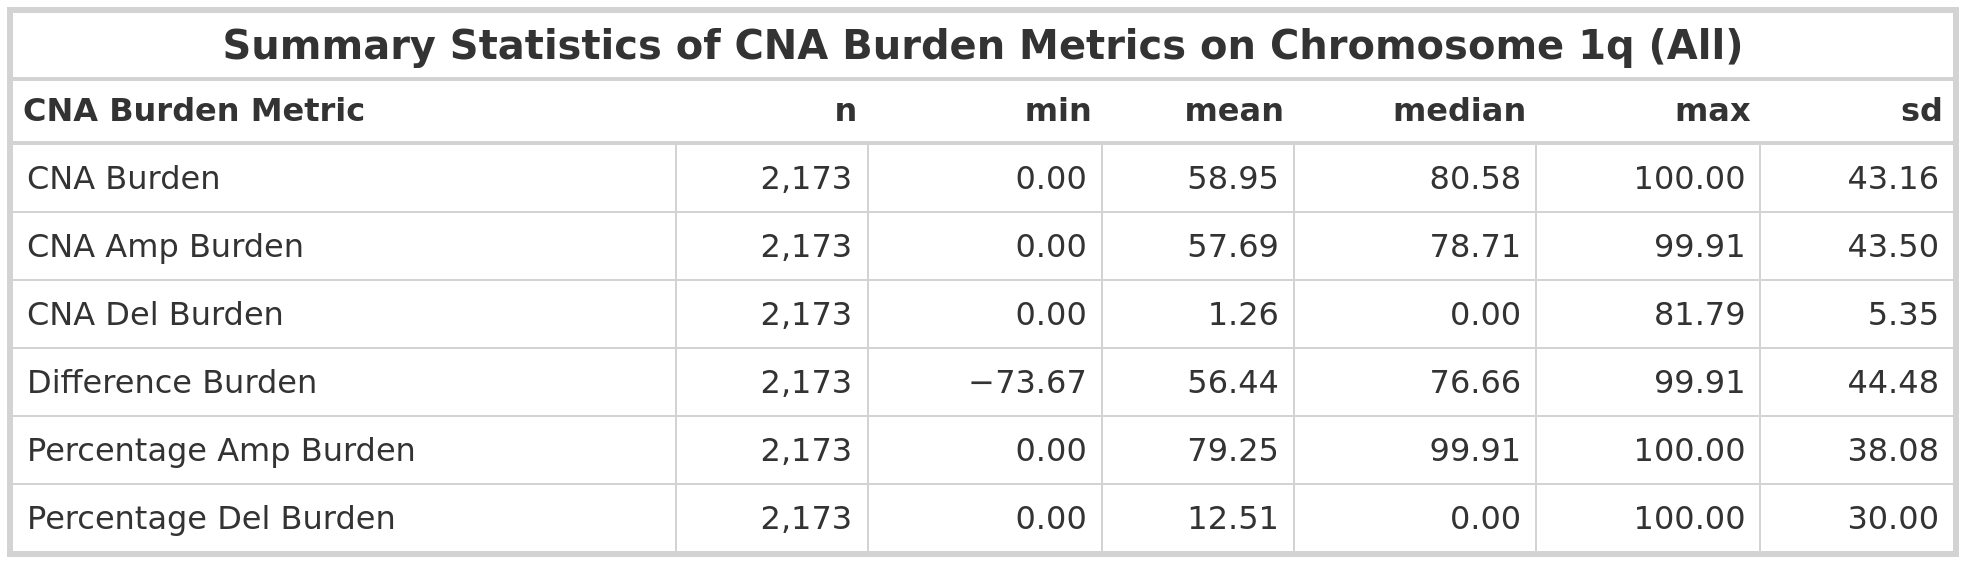
\includegraphics[width = 0.98\textwidth]{../tables/Chapter_2/CNA_Burden_Metric_All_Chr1q_Summary.png}
\label{tab:Burden_All_Chr1q}
\end{table}

\begin{table}[!ht]
\center
\caption[Summary statistics of the CNA Burden metrics on chromosome 1q where only complete cases are used.]{Summary statistics of the CNA Burden metrics on chromosome 1q where only complete cases are used.}
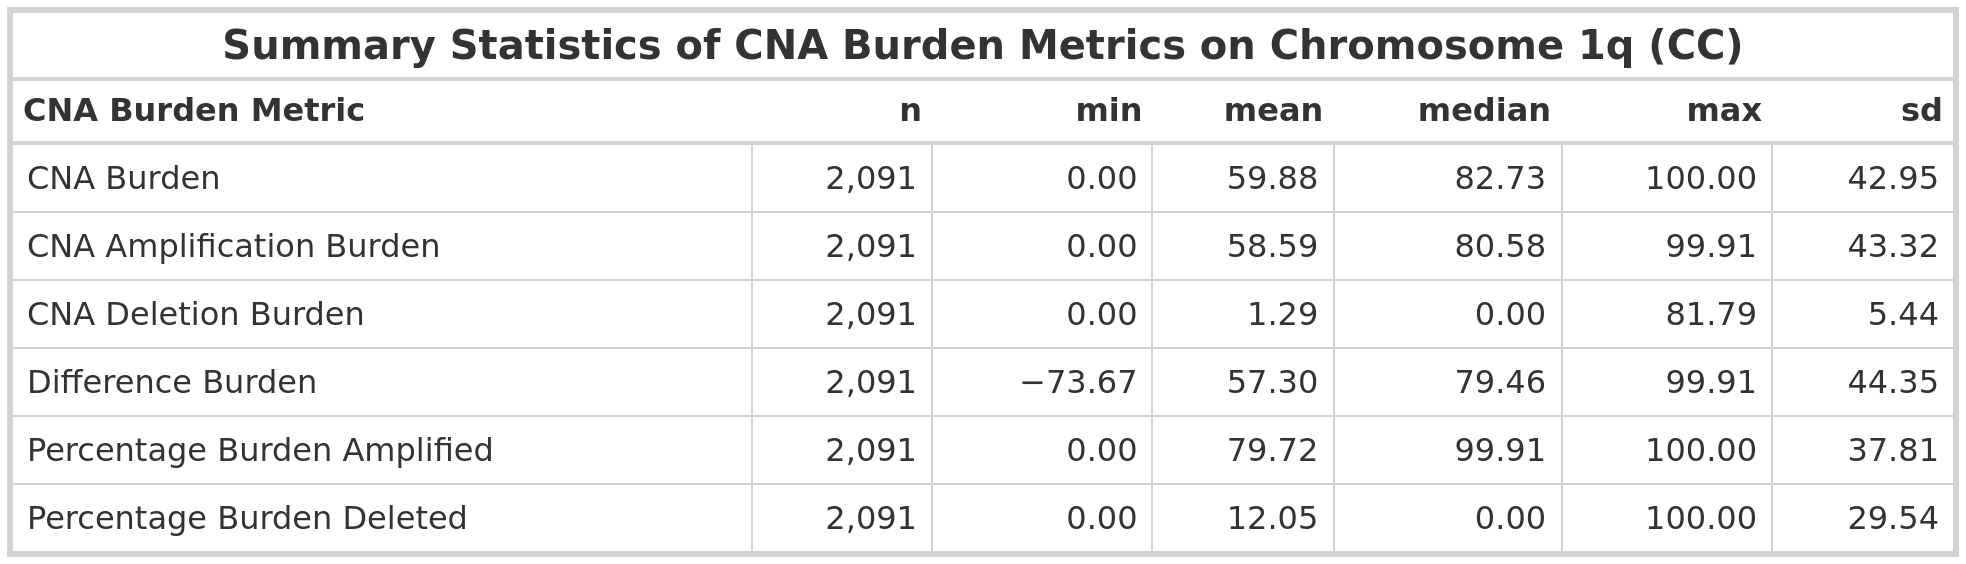
\includegraphics[width = 0.98\textwidth]{../tables/Chapter_2/CNA_Burden_Metric_CCA_Chr1q_Summary.png}
\label{tab:Burden_CCA_Chr1q}
\end{table}

\begin{figure}[!ht]
\center
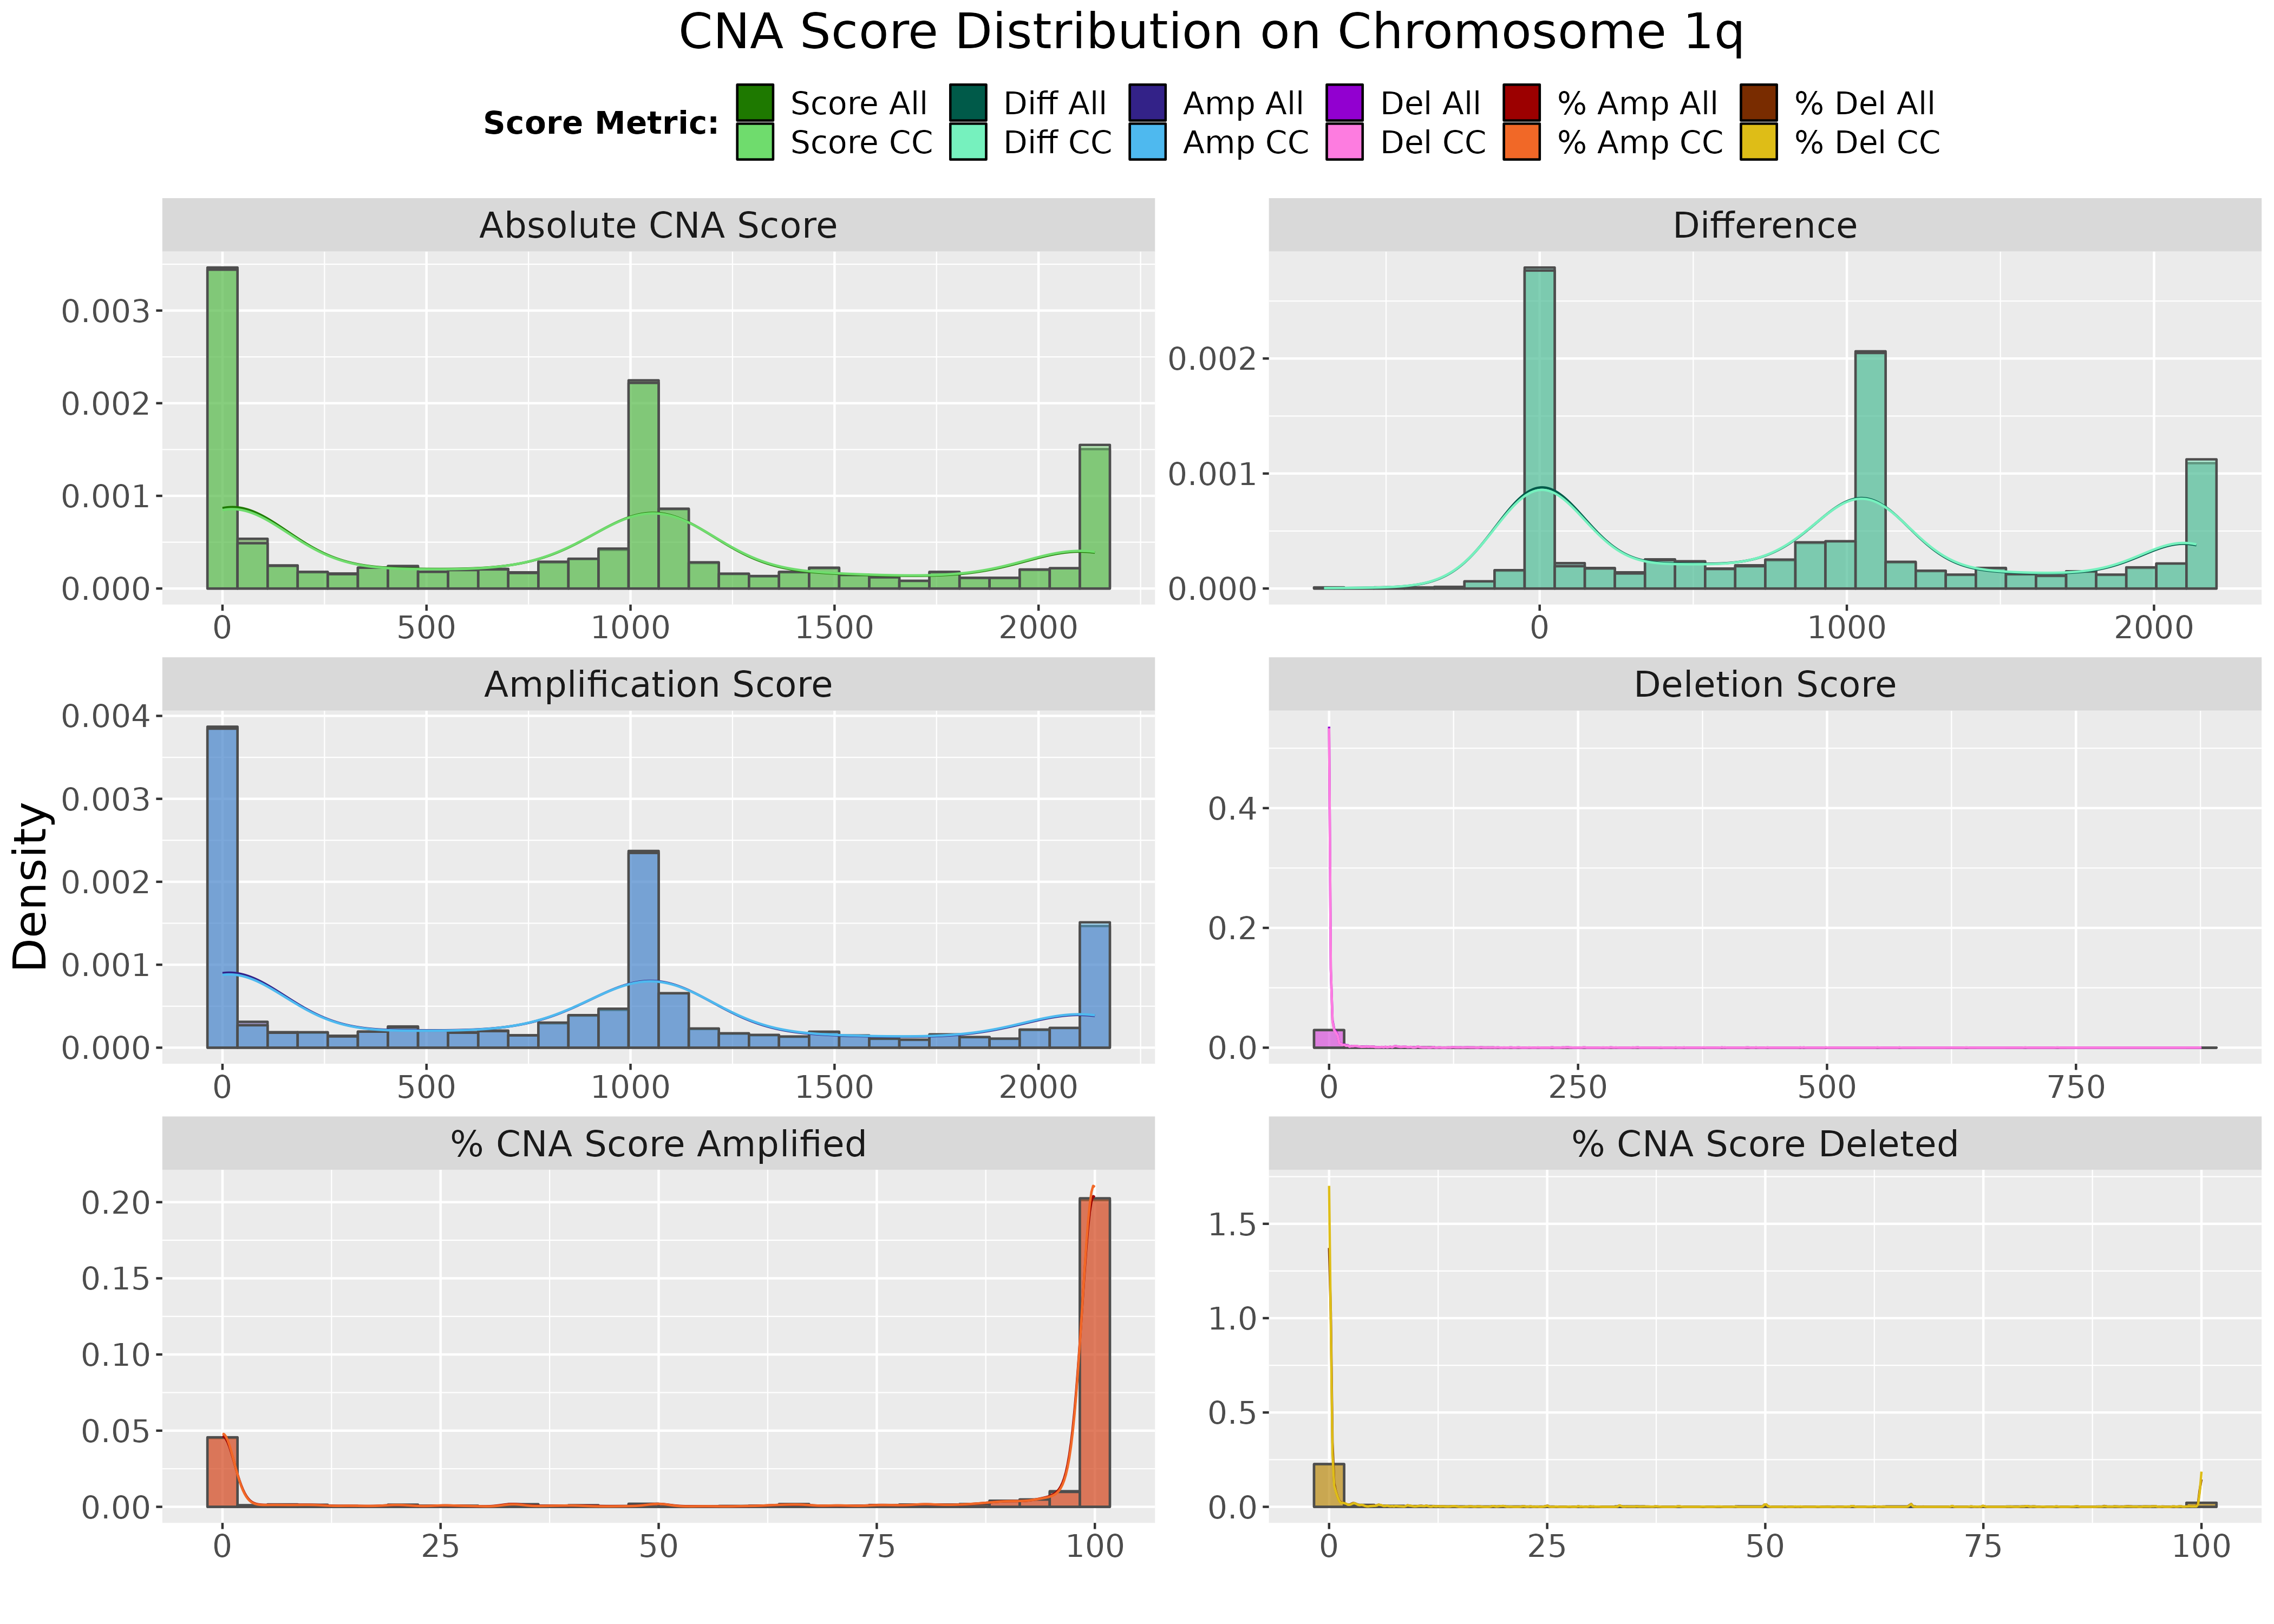
\includegraphics[width = 0.96\textwidth]{../figures/Chapter_2/CNA_Score_Comparative_Density_Chr1q.png}
\caption[Density plots for each CNA Score metric on chromosome 1q.]{Density plots for each CNA Score metric on chromosome 1q. Each facet contains density plots for both the complete-case CNA Score metric and the CNA Score metric calculated using all available data.}
\label{fig:Score_Comp_Dense_Chr1q}
\end{figure}

\begin{figure}[!ht]
\center
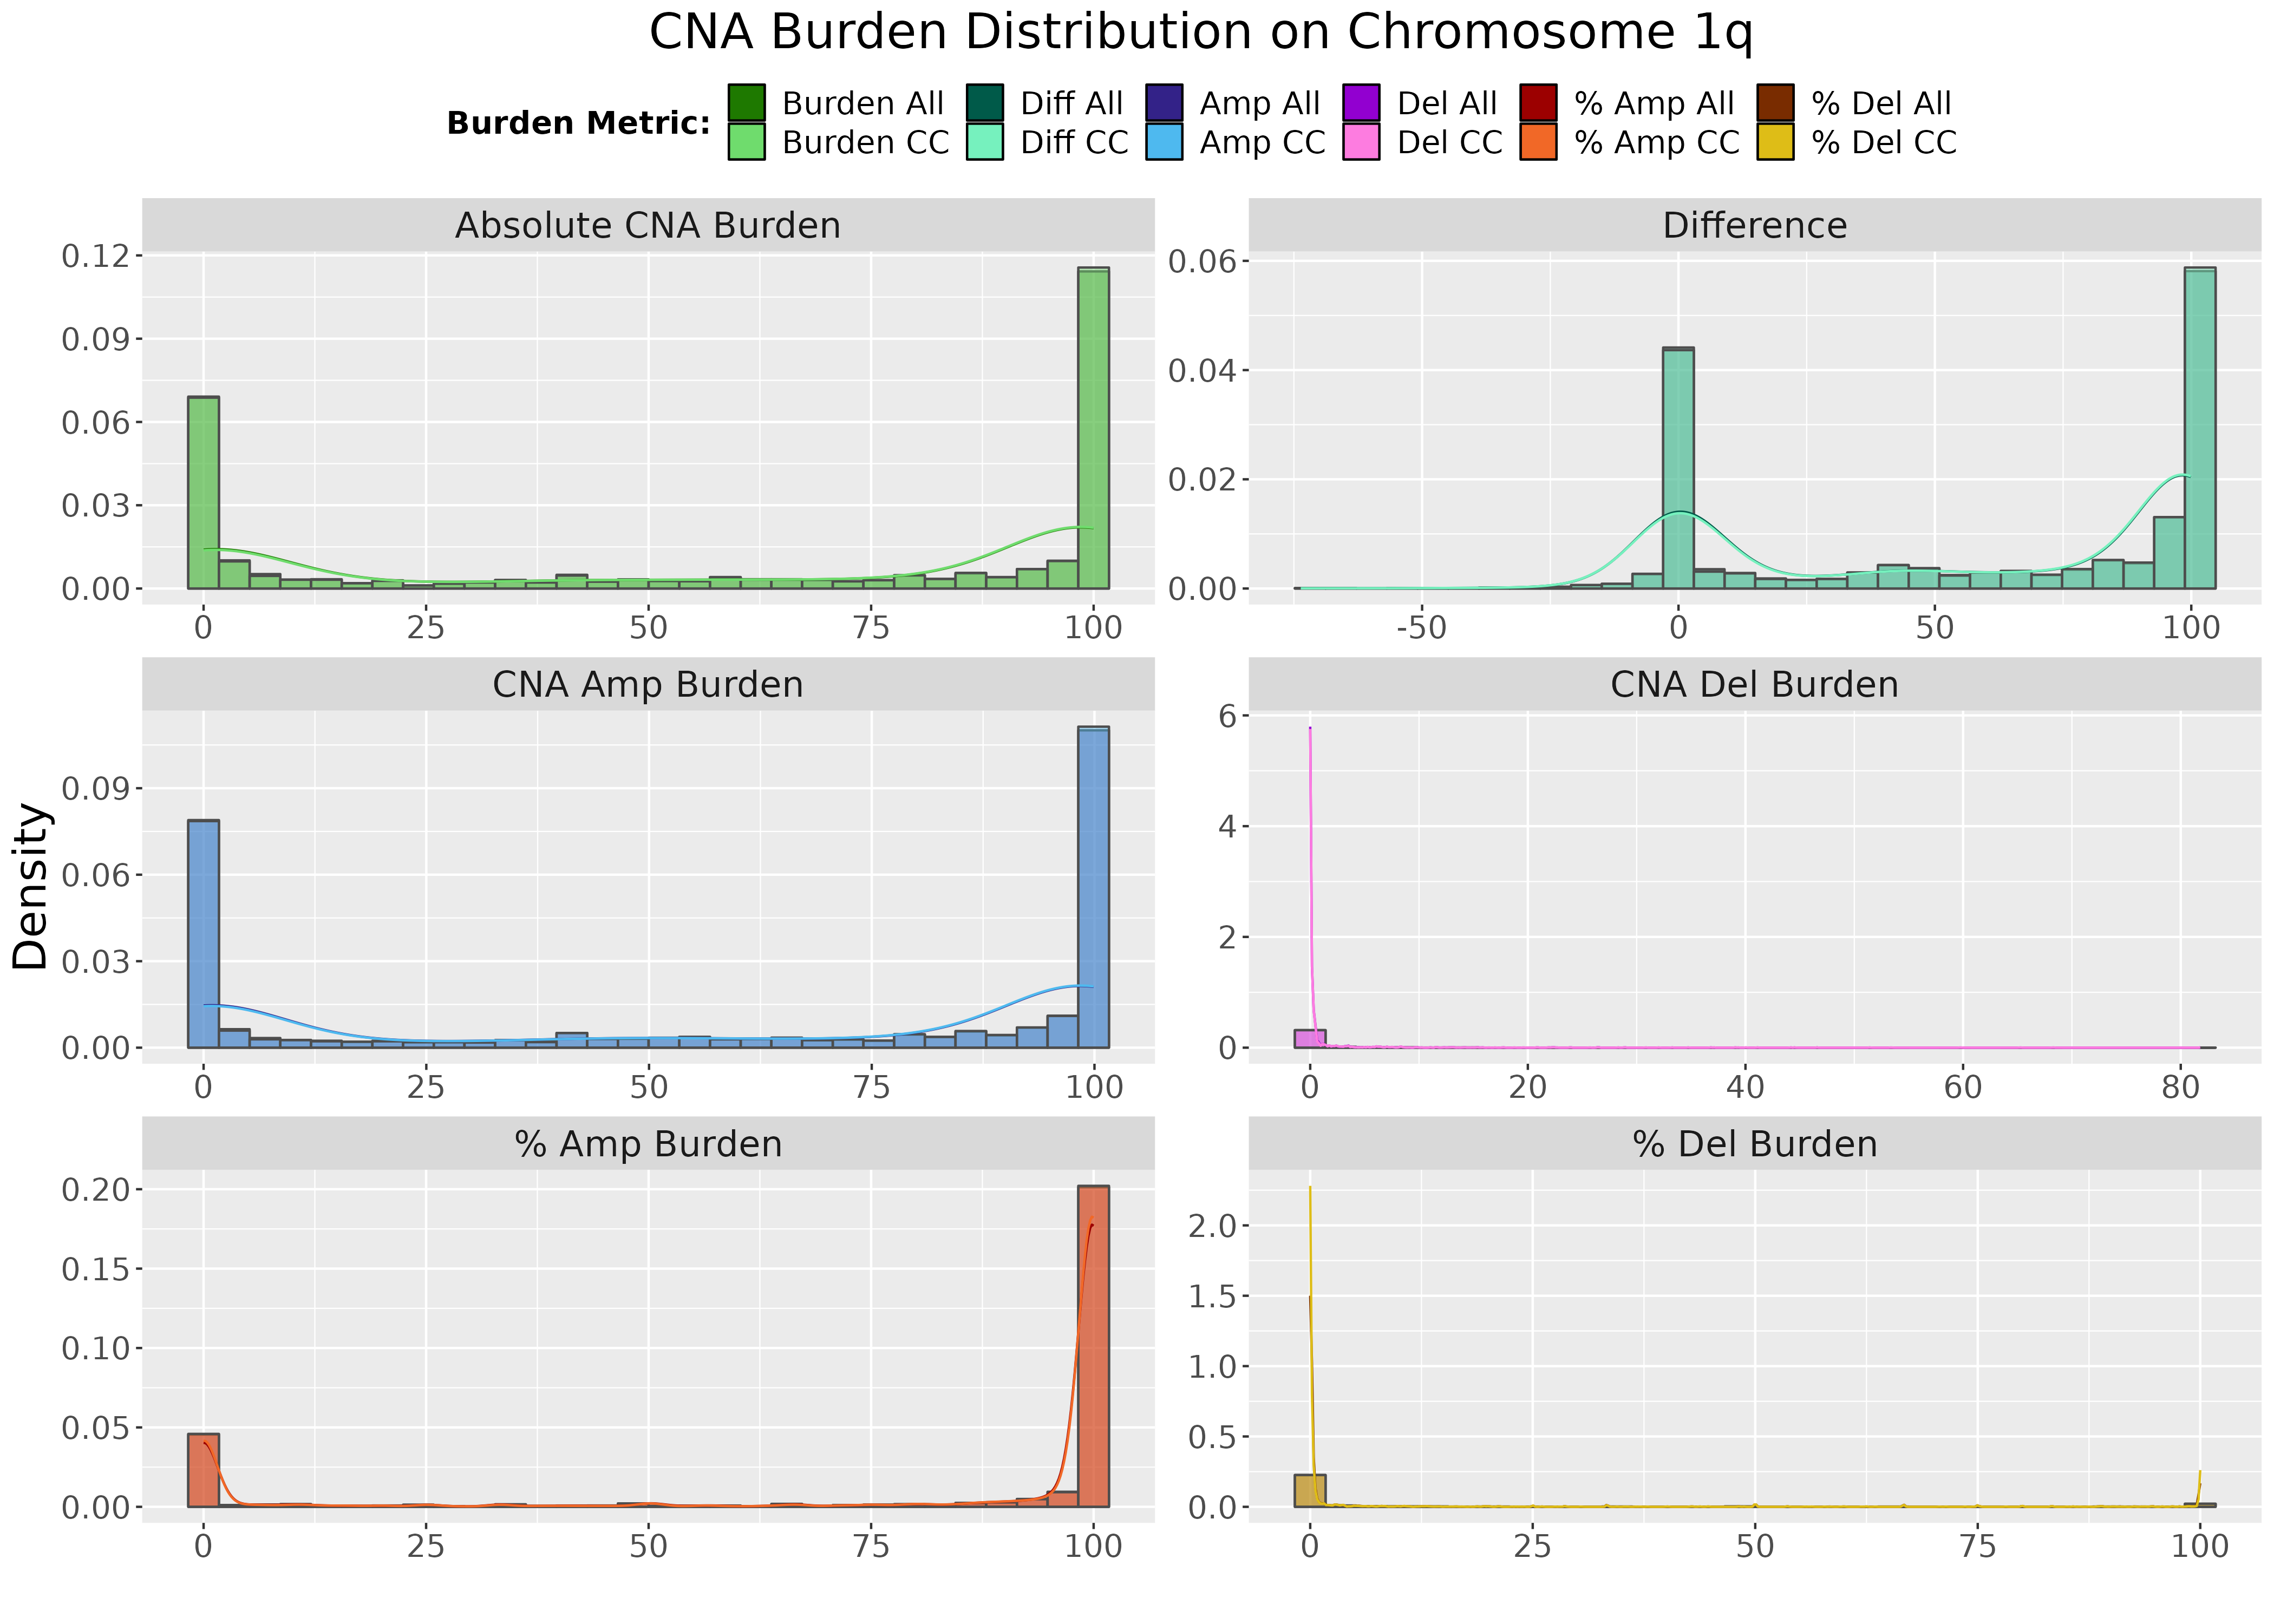
\includegraphics[width = 0.96\textwidth]{../figures/Chapter_2/CNA_Burden_Comparative_Density_Chr1q.png}
\caption[Density plots for each CNA Burden metric on chromosome 1q.]{Density plots for each CNA Burden metric on chromosome 1q. Each facet contains density plots for both the complete-case CNA Burden metric and the CNA Burden metric calculated using all available data.}
\label{fig:Burden_Comp_Dense_Chr1q}
\end{figure}
\clearpage 

\subsection{CNA Metric Distributions within Molecular Subtype Classifications}
\label{LGI}
The calculated CNA Score and Burden metrics are cross-referenced against breast cancer subtype classifications, PAM50 subtype and IntClust, to determine if observed distributions of metrics differed comparing these stratified cohorts of patients. Within the METABRIC cohort there are 1,974 patients for which CNA data and PAM50 subtype information are available and 1,980 patients for which CNA data and IntClust information are available (Table \ref{Clinchar}). The 529 patients missing both PAM50 and IntClust information did not have any gene expression data available meaning they could not be allocated PAM50 or IntClust, while six patients had IntClust information but were categorised as PAM50 “NC” and subsequently recoded as NA. We present distributions of the global CNA metrics across molecular classifications in section \ref{ObsDis} and distributions of the chromosome arm CNA metrics across molecular classifications in section \ref{ObsDis1}.

\subsubsection{Observed Distributions for Global CNA Metrics across Molecular Subtype Classifications}
\label{ObsDis}
The observed distribution of the six CNA Score metrics, for patients stratified by PAM50 subtype, is displayed in Figure \ref{fig:CNA-Score-Metric-Boxplots-P50}, and Figure \ref{fig:CNA-Burden-Metric-Boxplots-P50} displays the six CNA Burden metrics. Also provided with Figures \ref{fig:CNA-Score-Metric-Boxplots-P50} and \ref{fig:CNA-Burden-Metric-Boxplots-P50} are the Benjamini-Hochberg (BH) adjusted p-values for the Kruskal-Wallis test for any difference in the distribution of a metric comparing the groups of patients stratified by PAM50 subtype. 

These visualisations and accompanying statistical tests (Figure \ref{fig:CNA-Score-Metric-Boxplots-P50} and Figure \ref{fig:CNA-Burden-Metric-Boxplots-P50}) indicate that some significant difference exists comparing each of the CNA metric distributions across PAM50 subtype (Kruskal-Wallis adjusted $p<0.0001$). Dunn's Test, a post-hoc test for Kruskal-Wallis, is then applied to each CNA metric performing pairwise comparisons to determine which groups are significantly different in mean rank scores (Tables \ref{tab:DT_Score_1} and \ref{tab:DT_Burden_1}). The distribution of CNA Score and Burden metrics in Basal patients is significantly different from all other subtypes (Tables \ref{tab:DT_Score_1} and \ref{tab:DT_Burden_1}). Basal patients display the highest Absolute CNA Scores and CNA Burden across all subtypes ($p<0.0001$) indicating higher levels of GI when compared to other subtypes. In line with this, the Basal patients display the highest CNA Amp and Del Score and Burden across all subtypes ($p<0.001$ for each comparison).

The HER2 and Luminal B subtypes have the 2nd and 3rd highest Absolute CNA Score and Burden, CNA Amp Score and Burden and CNA Del Score and Burden, respectively. While the shape and spread of these metric distributions appear quite similar, the HER2 subtype displays slightly higher levels of Absolute CNA Score and Burden ($p = 0.01$). This is also observed for the CNA Del metrics, where HER2 patients have higher levels of deletions than Luminal B patients ($p = 0.01$), but not the CNA Amp metrics ($p = 0.41$ and $p = 0.47$). When comparing the Luminal A and Luminal B patients, it is observed that Luminal B patients have significantly higher levels of instability across all metrics ($p<0.0001$). The Luminal A, Normal and Claudin-low patients display the lowest CNA Score and Burden metrics. The Normal and Claudin-low subtypes display no significant difference for the total, amplification and deletion CNA Score and Burden metrics ($p>0.05$). All Luminal A and Claudin-low densities, apart from the CNA Amp metric distributions, are not significantly different from each other in these subtypes ($p>0.05$). Luminal A patients display significantly higher levels of amplifications when compared with Normal and Claudin-low subtypes ($p < 0.0001$, Tables \ref{tab:DT_Score_1} and \ref{tab:DT_Burden_1}). 

Focusing on the direct comparison of levels of amplification to deletion within each PAM50 subtype, Figures \ref{fig:CNA-Score-Metric-Boxplots-P50-AmpDel} and \ref{fig:CNA-Burden-Metric-Boxplots-P50-AmpDel}, the subtypes known to be associated with poorer survival outcome, i.e. Basal, HER2 and Luminal B, have significantly higher levels of deletion burden than amplification burden ($p<0.0001$). Conversely PAM50 subtypes with better survival prognosis either display significantly more amplifications, Luminal A ($p < 0.01$), or no significant difference in the levels of amplifications and deletions, Normal and Claudin-low ($p > 0.05$).

\vfill
\begin{figure}[!h]
\center
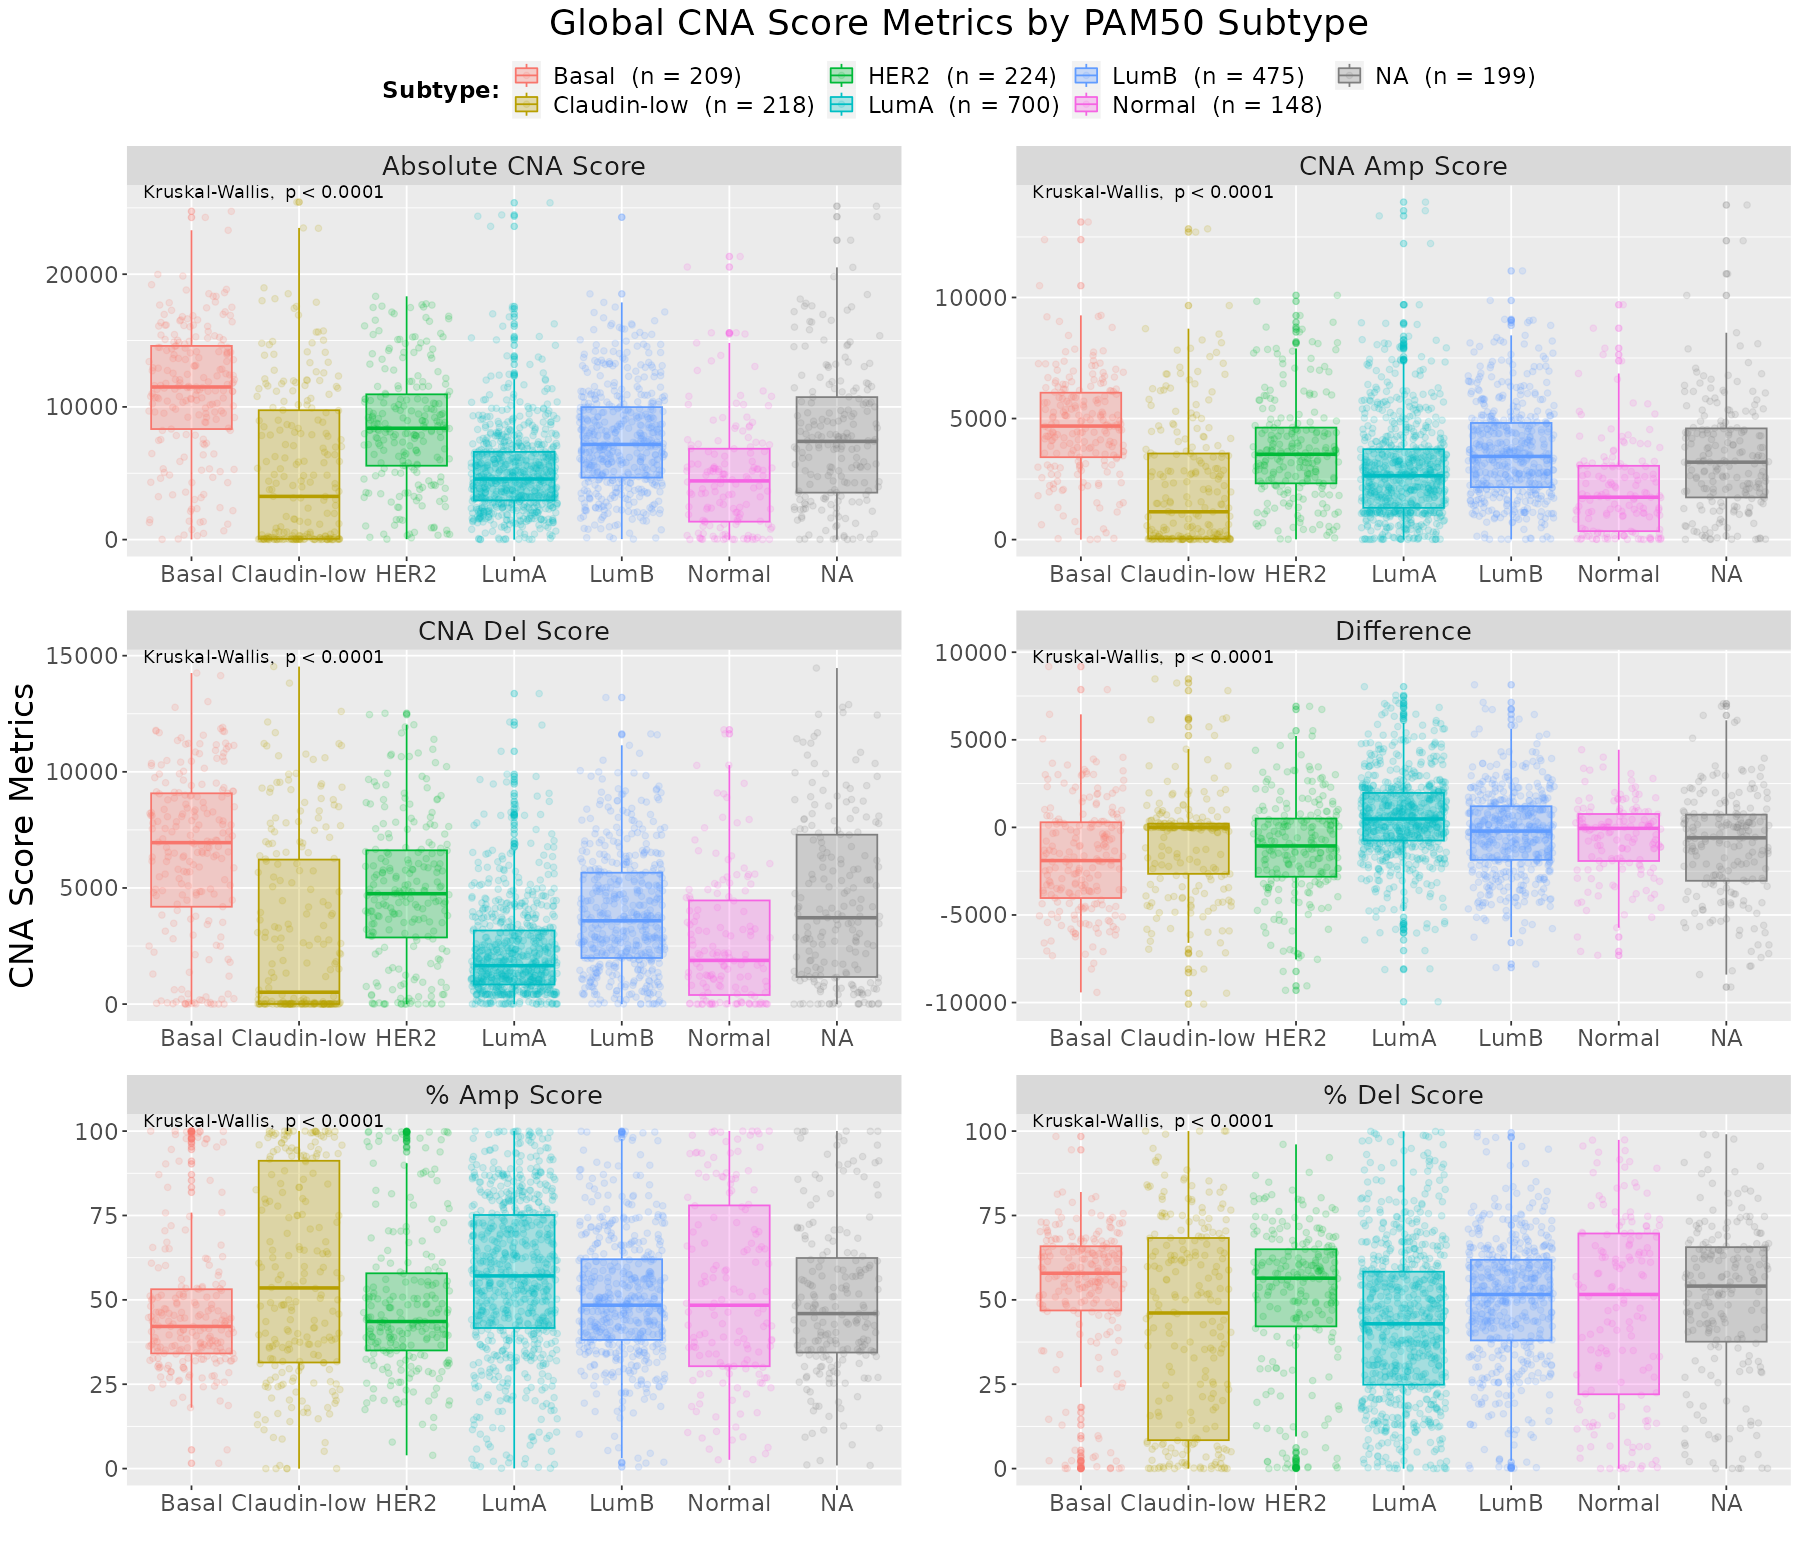
\includegraphics[width=1\textwidth]{../figures/Chapter_2/Global_CNA_Score_Metrics_Across_PAM50.png}
\caption[Boxplots for each CNA Score metric by PAM50 subtype.]{Boxplots for each CNA Score metric by PAM50 subtype. Each facet contains boxplots for the CNA Score metrics calculated using all available data accompanied by Benjamini-Hochberg adjusted Kruskal-Wallis p-values. NA denotes METABRIC patients missing PAM50 information.}
\label{fig:CNA-Score-Metric-Boxplots-P50}
\end{figure}
\vfill

\begin{figure}[!ht]
\center
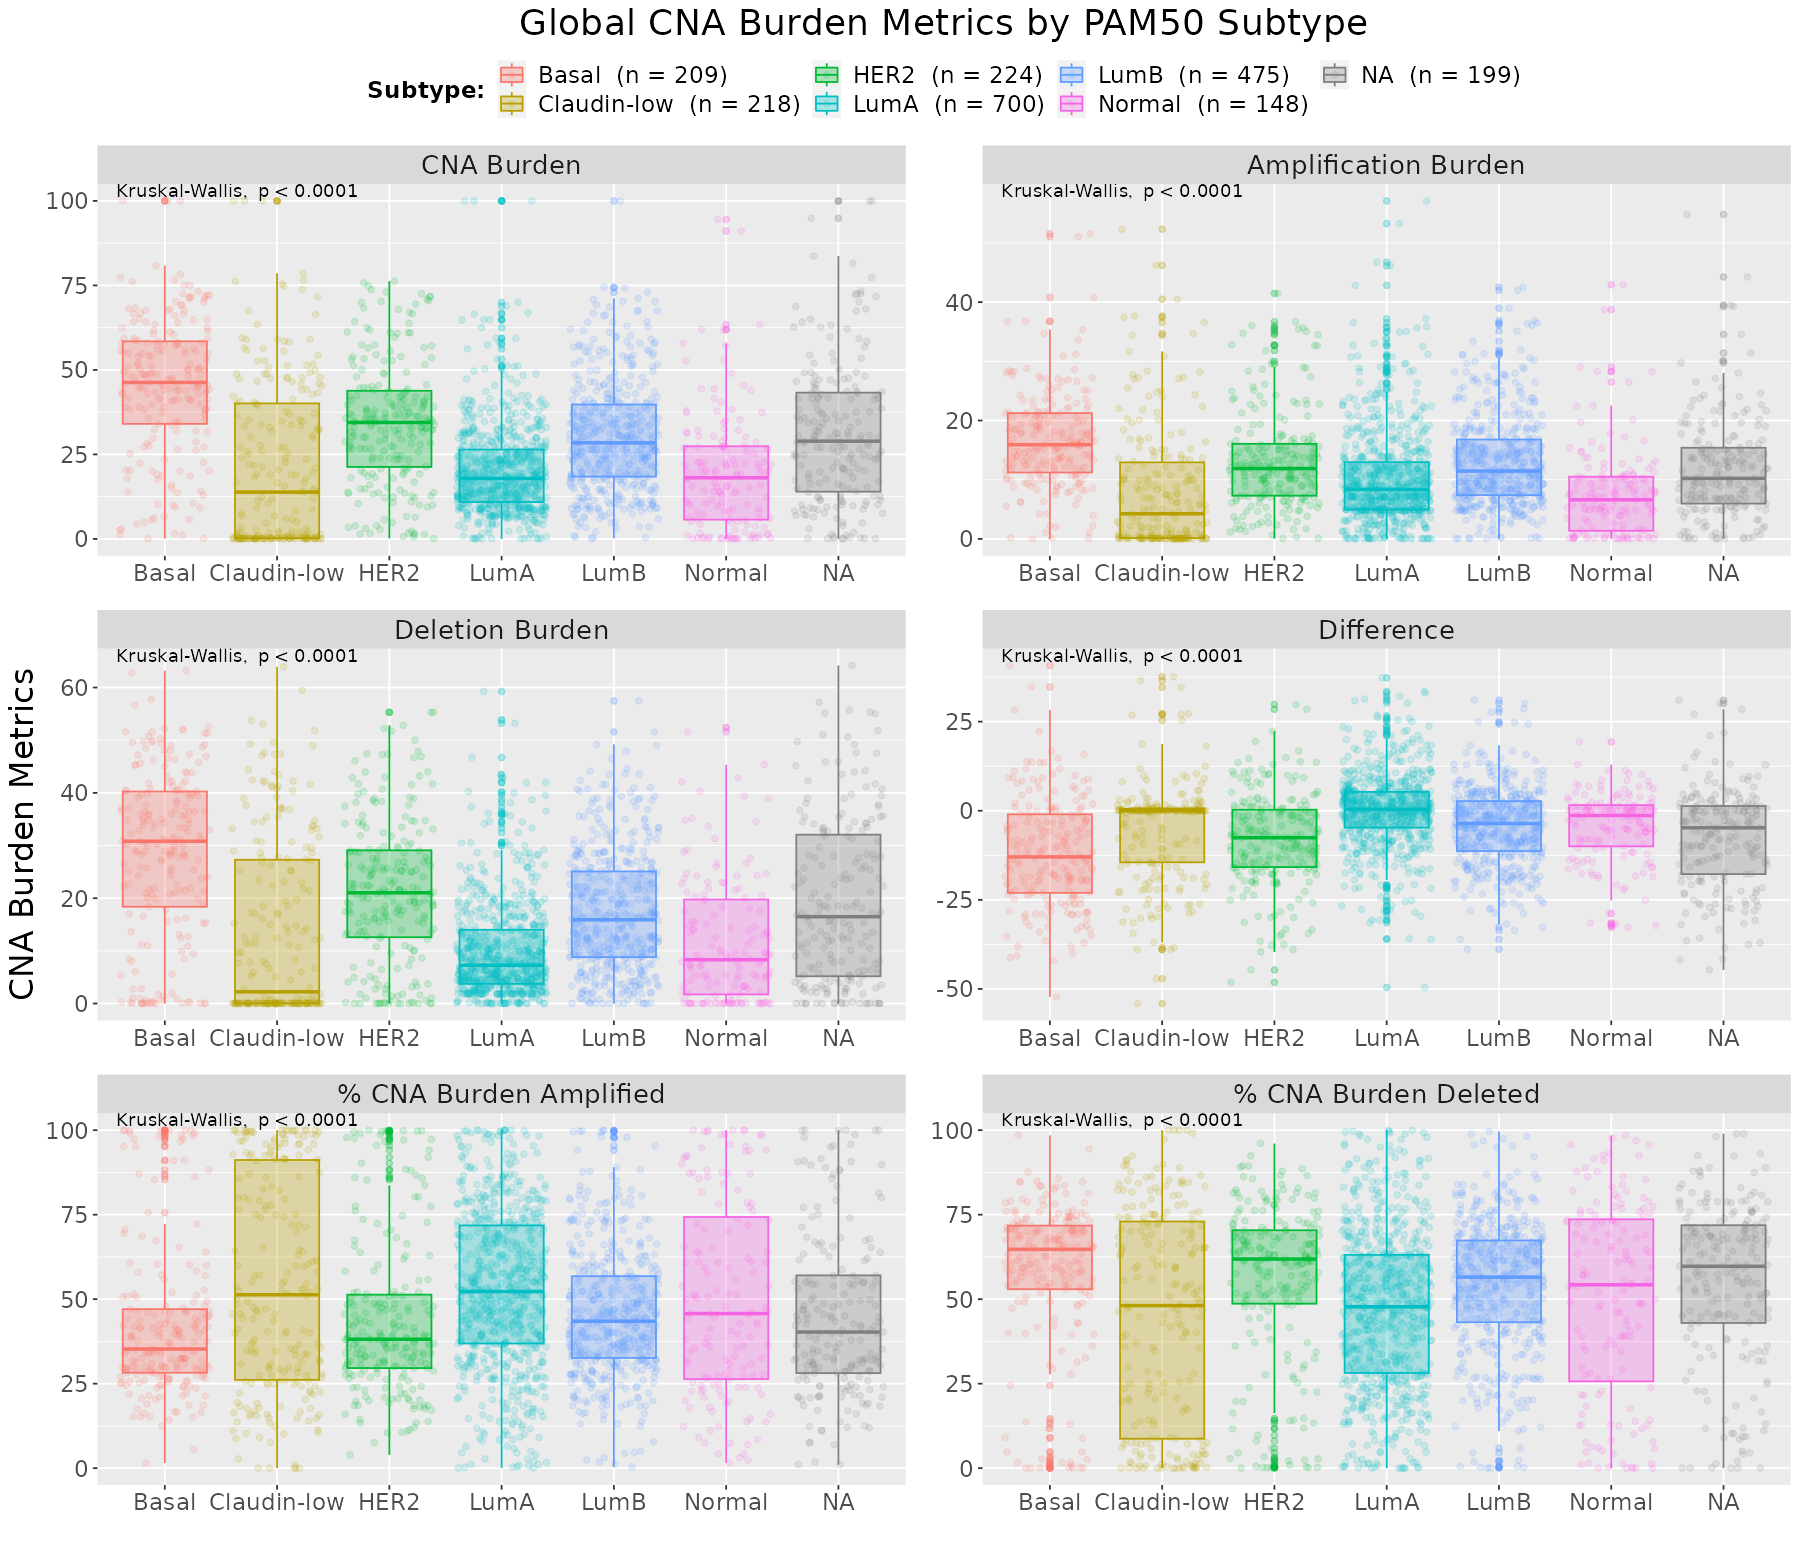
\includegraphics[width=1\textwidth]{../figures/Chapter_2/Global_CNA_Burden_Metrics_Across_PAM50.png}
\caption[Boxplots for each CNA Burden metric by PAM50 subtype.]{Boxplots for each CNA Burden metric by PAM50 subtype. Each facet contains boxplots for the CNA Burden metrics calculated using all available data accompanied by Benjamini-Hochberg adjusted Kruskal-Wallis p-values. NA denotes METABRIC patients missing PAM50 information.}
\label{fig:CNA-Burden-Metric-Boxplots-P50}
\end{figure}

\begin{table}[!ht]
\center
\caption[Comparisons of CNA Score metric distributions by PAM50 subtype.]{Comparisons of CNA Score metric distributions by PAM50 subtype. Z statistic and Benjamini-Hochberg adjusted p-value for each Dunn's test are shown.}
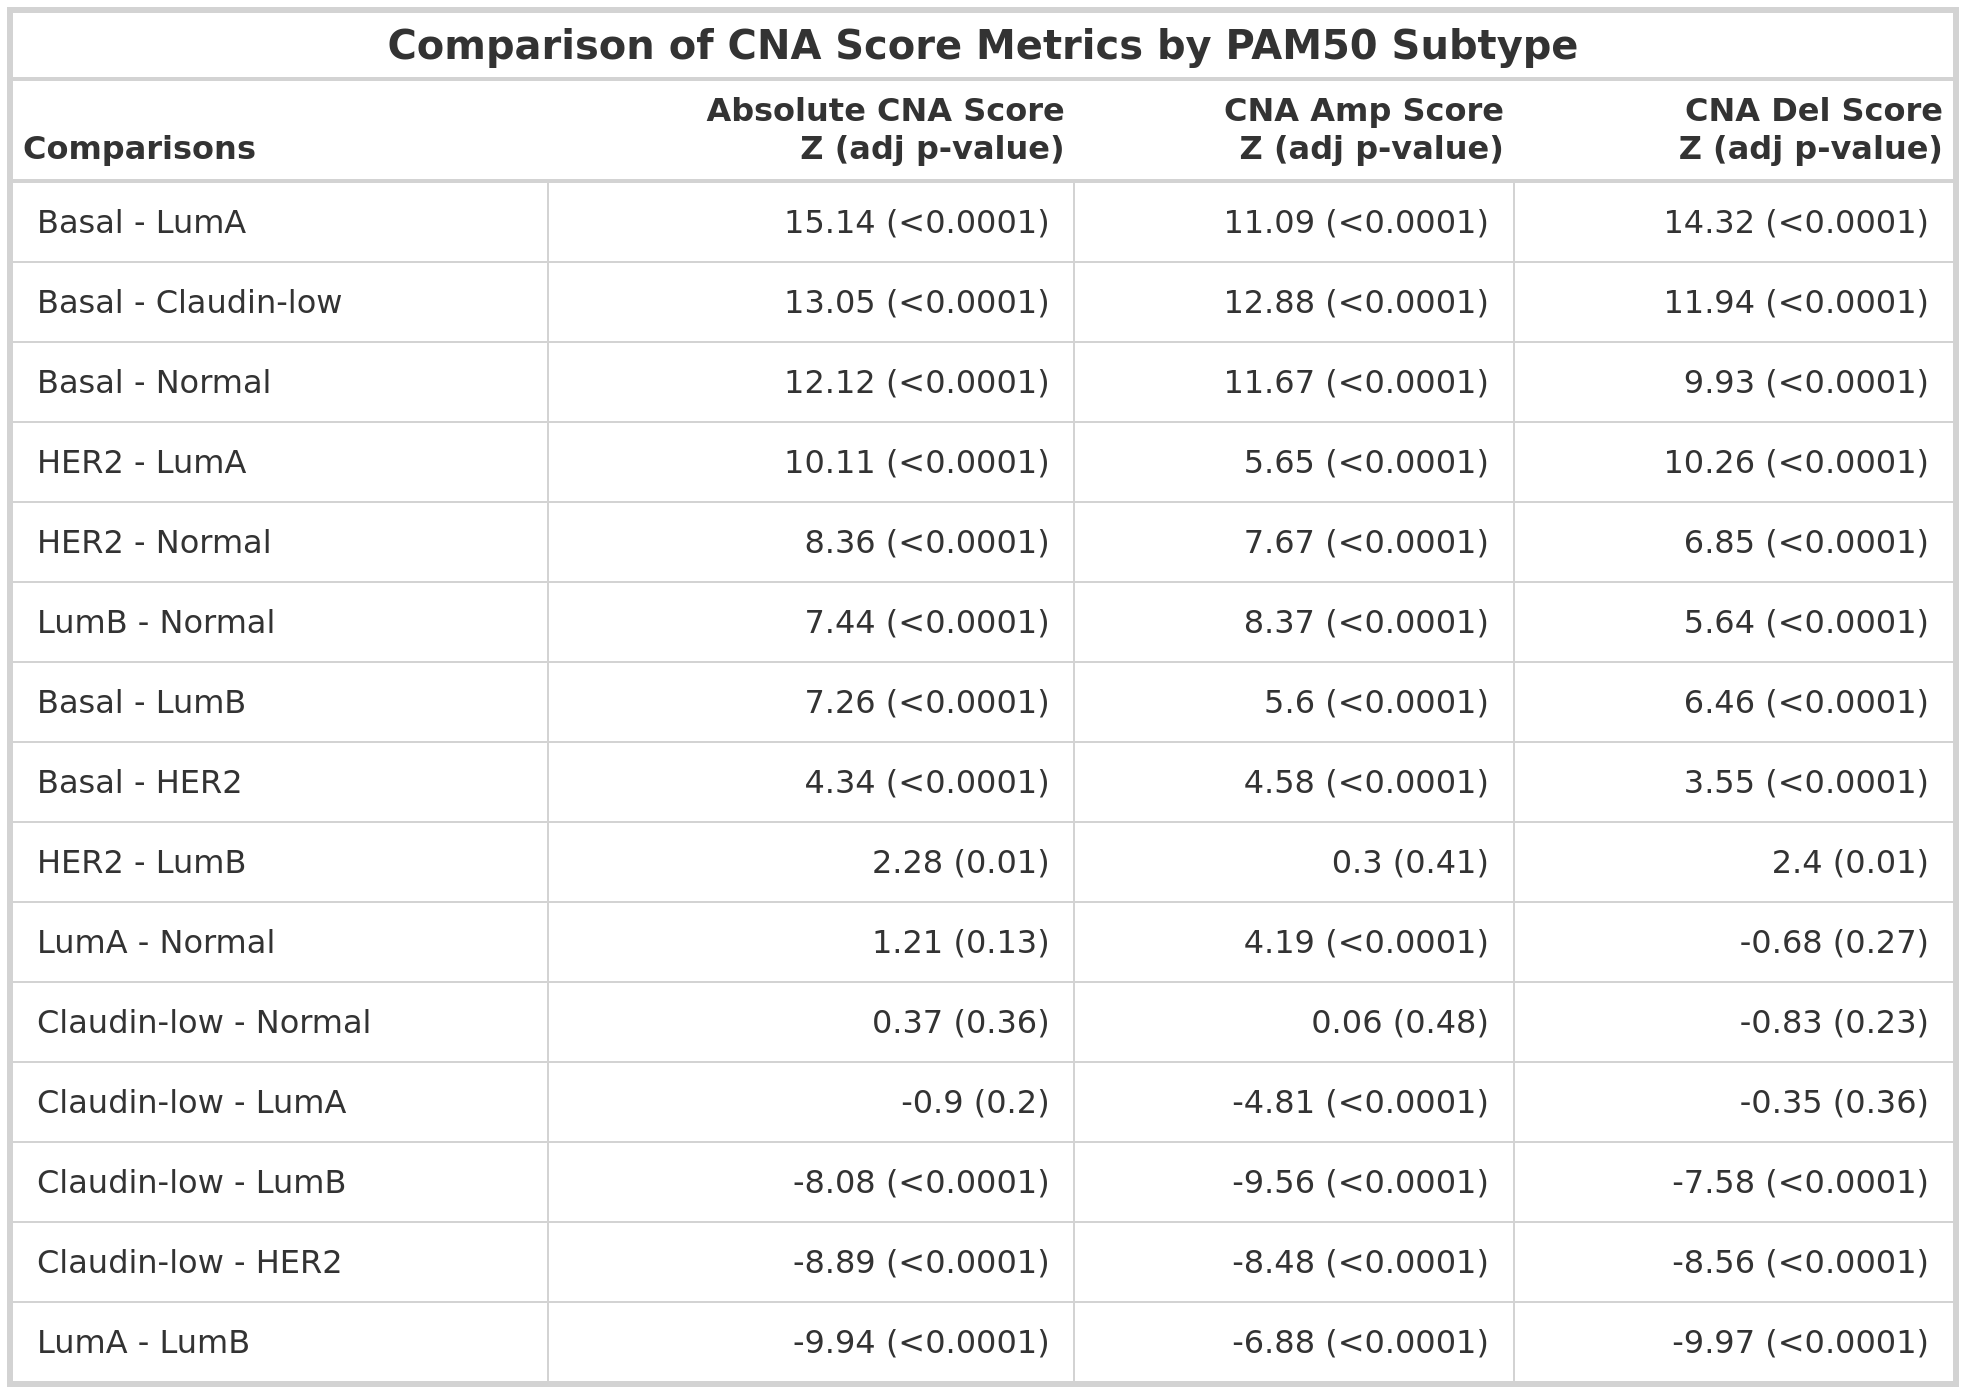
\includegraphics[width=0.98\textwidth]{../tables/Chapter_2/Global_CNA_Score_Metric_Comparisons.png}
\label{tab:DT_Score_1}
\end{table}

\begin{table}[!ht]
\center
\caption[Comparisons of CNA Burden metric distributions by PAM50 subtype.]{Comparisons of CNA Burden metric distributions by PAM50 subtype. Z statistic and Benjamini-Hochberg adjusted p-value for each Dunn's test are shown.}
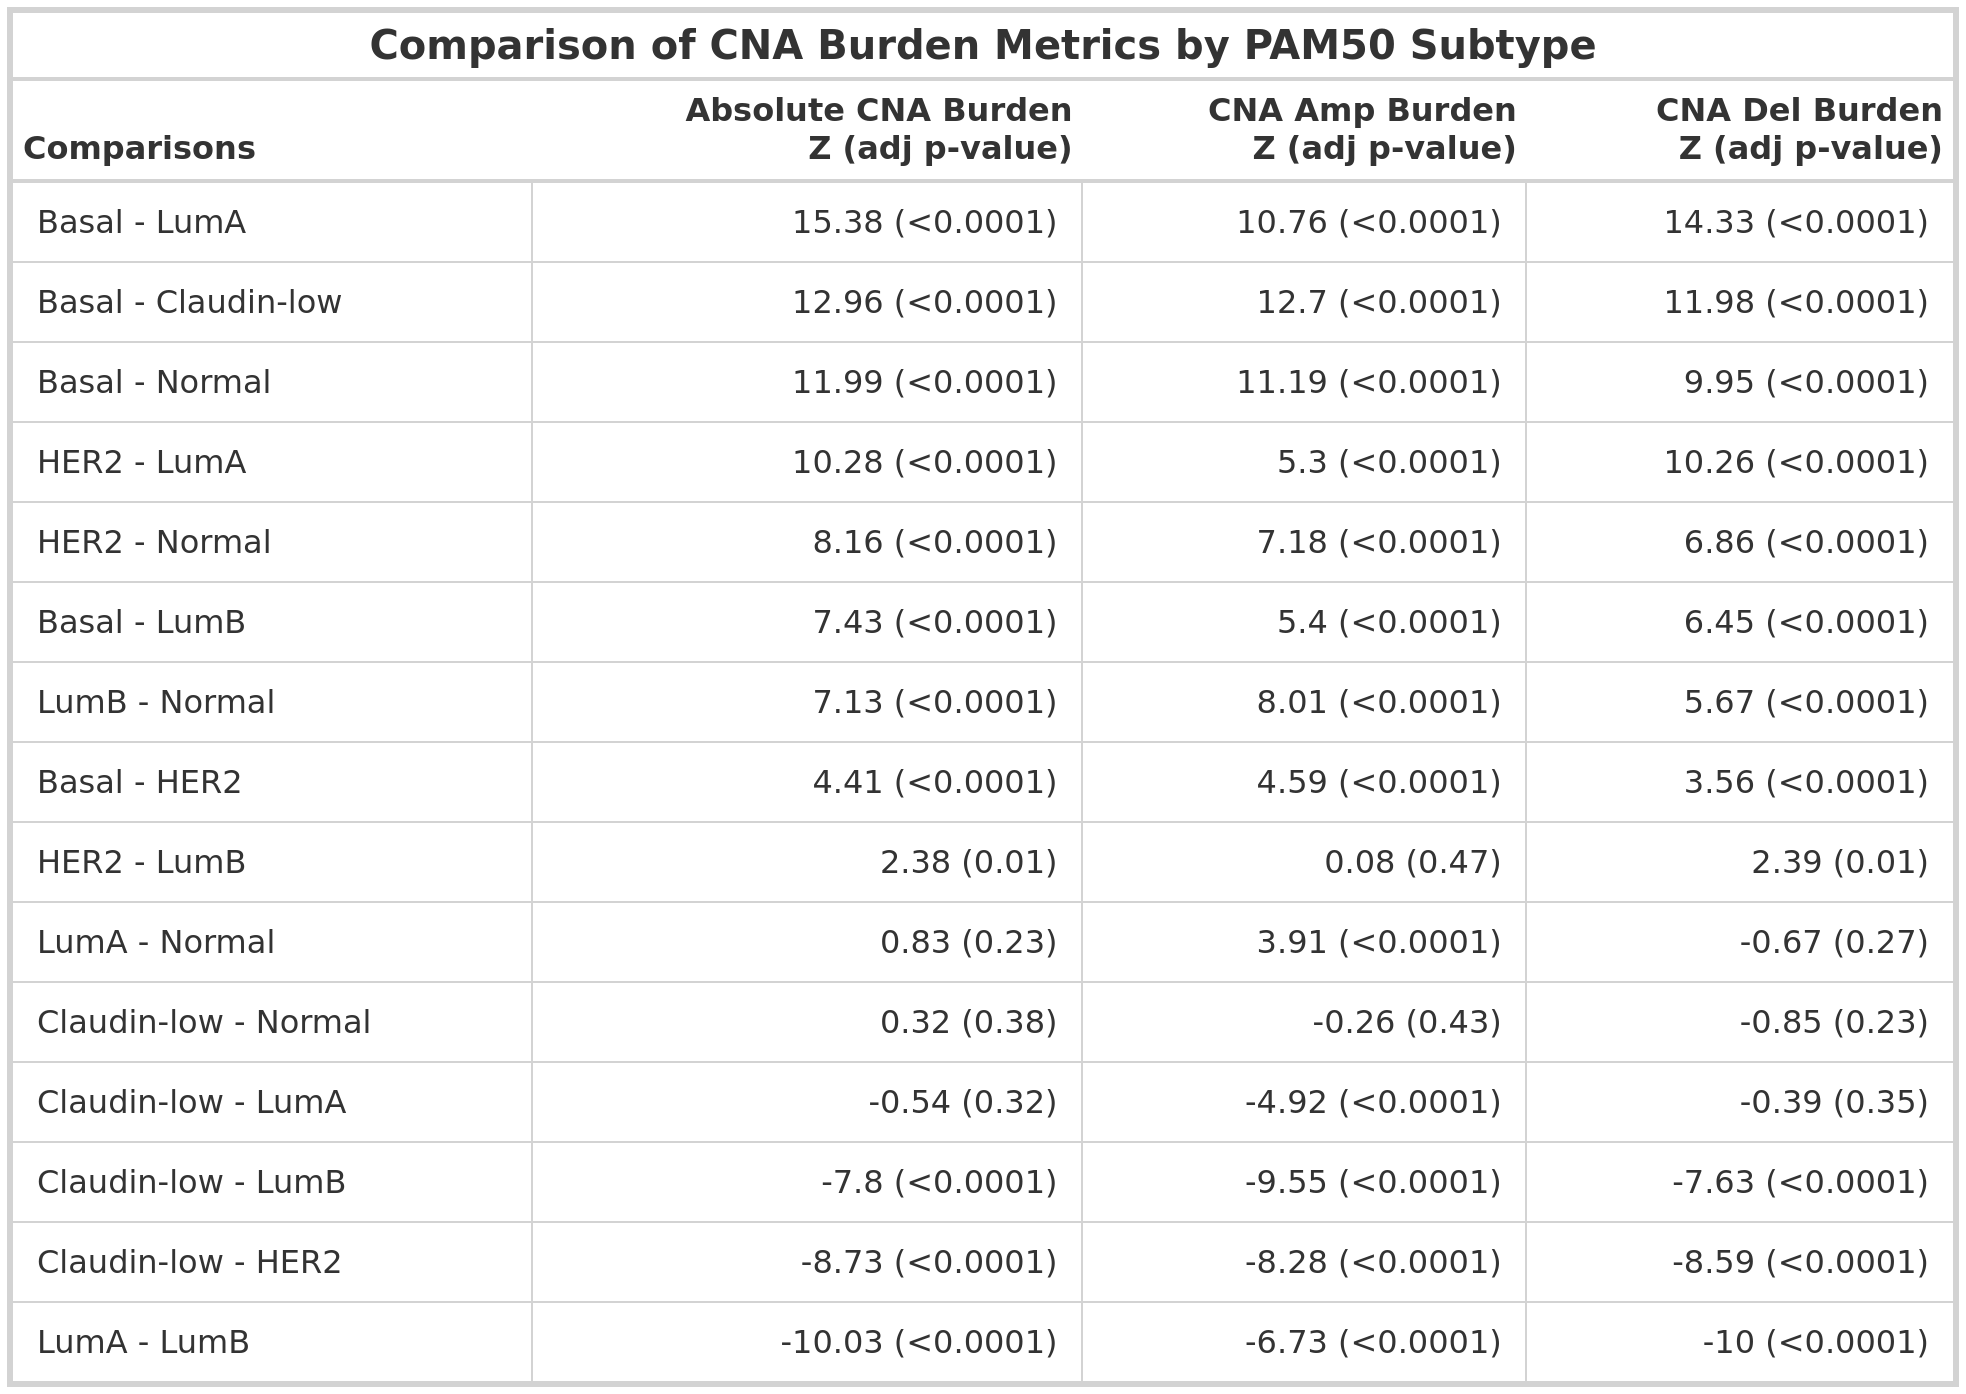
\includegraphics[width=0.98\textwidth]{../tables/Chapter_2/Global_CNA_Burden_Metric_Comparisons.png}
\label{tab:DT_Burden_1}
\end{table}

\begin{figure}[!ht]
\center
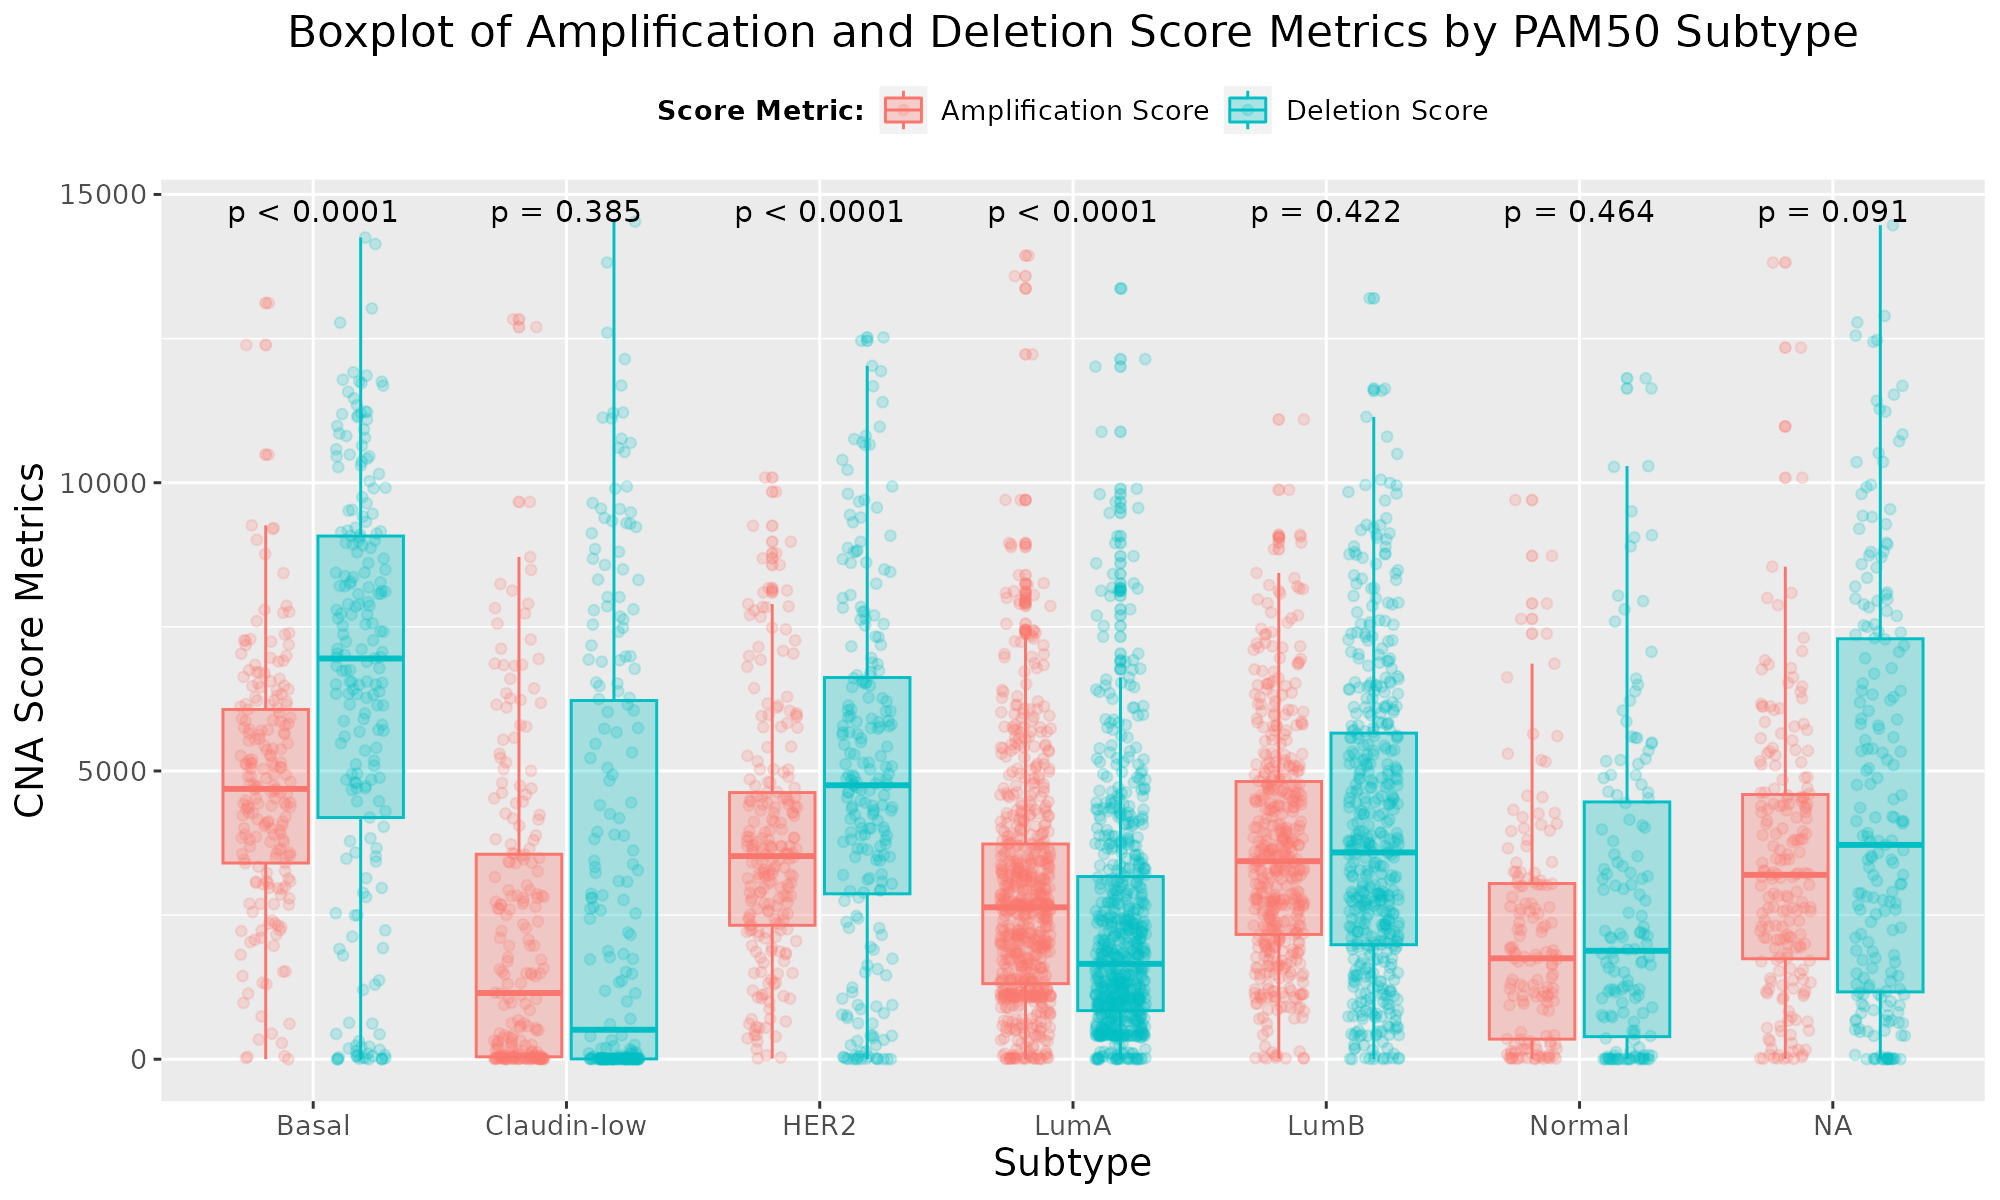
\includegraphics[width=1\textwidth]{../figures/Chapter_2/Global_CNA_Score_AmpDel_Across_PAM50.png}
\caption[Boxplots for each CNA Amp and CNA Del Score metric by PAM50 subtype.]{Boxplots for each CNA Amp and CNA Del Score metric by PAM50 subtype. Includes Benjamini-Hochberg adjusted Kruskal-Wallis p-values.}
\label{fig:CNA-Score-Metric-Boxplots-P50-AmpDel}
\end{figure}

\begin{figure}[!ht]
\center
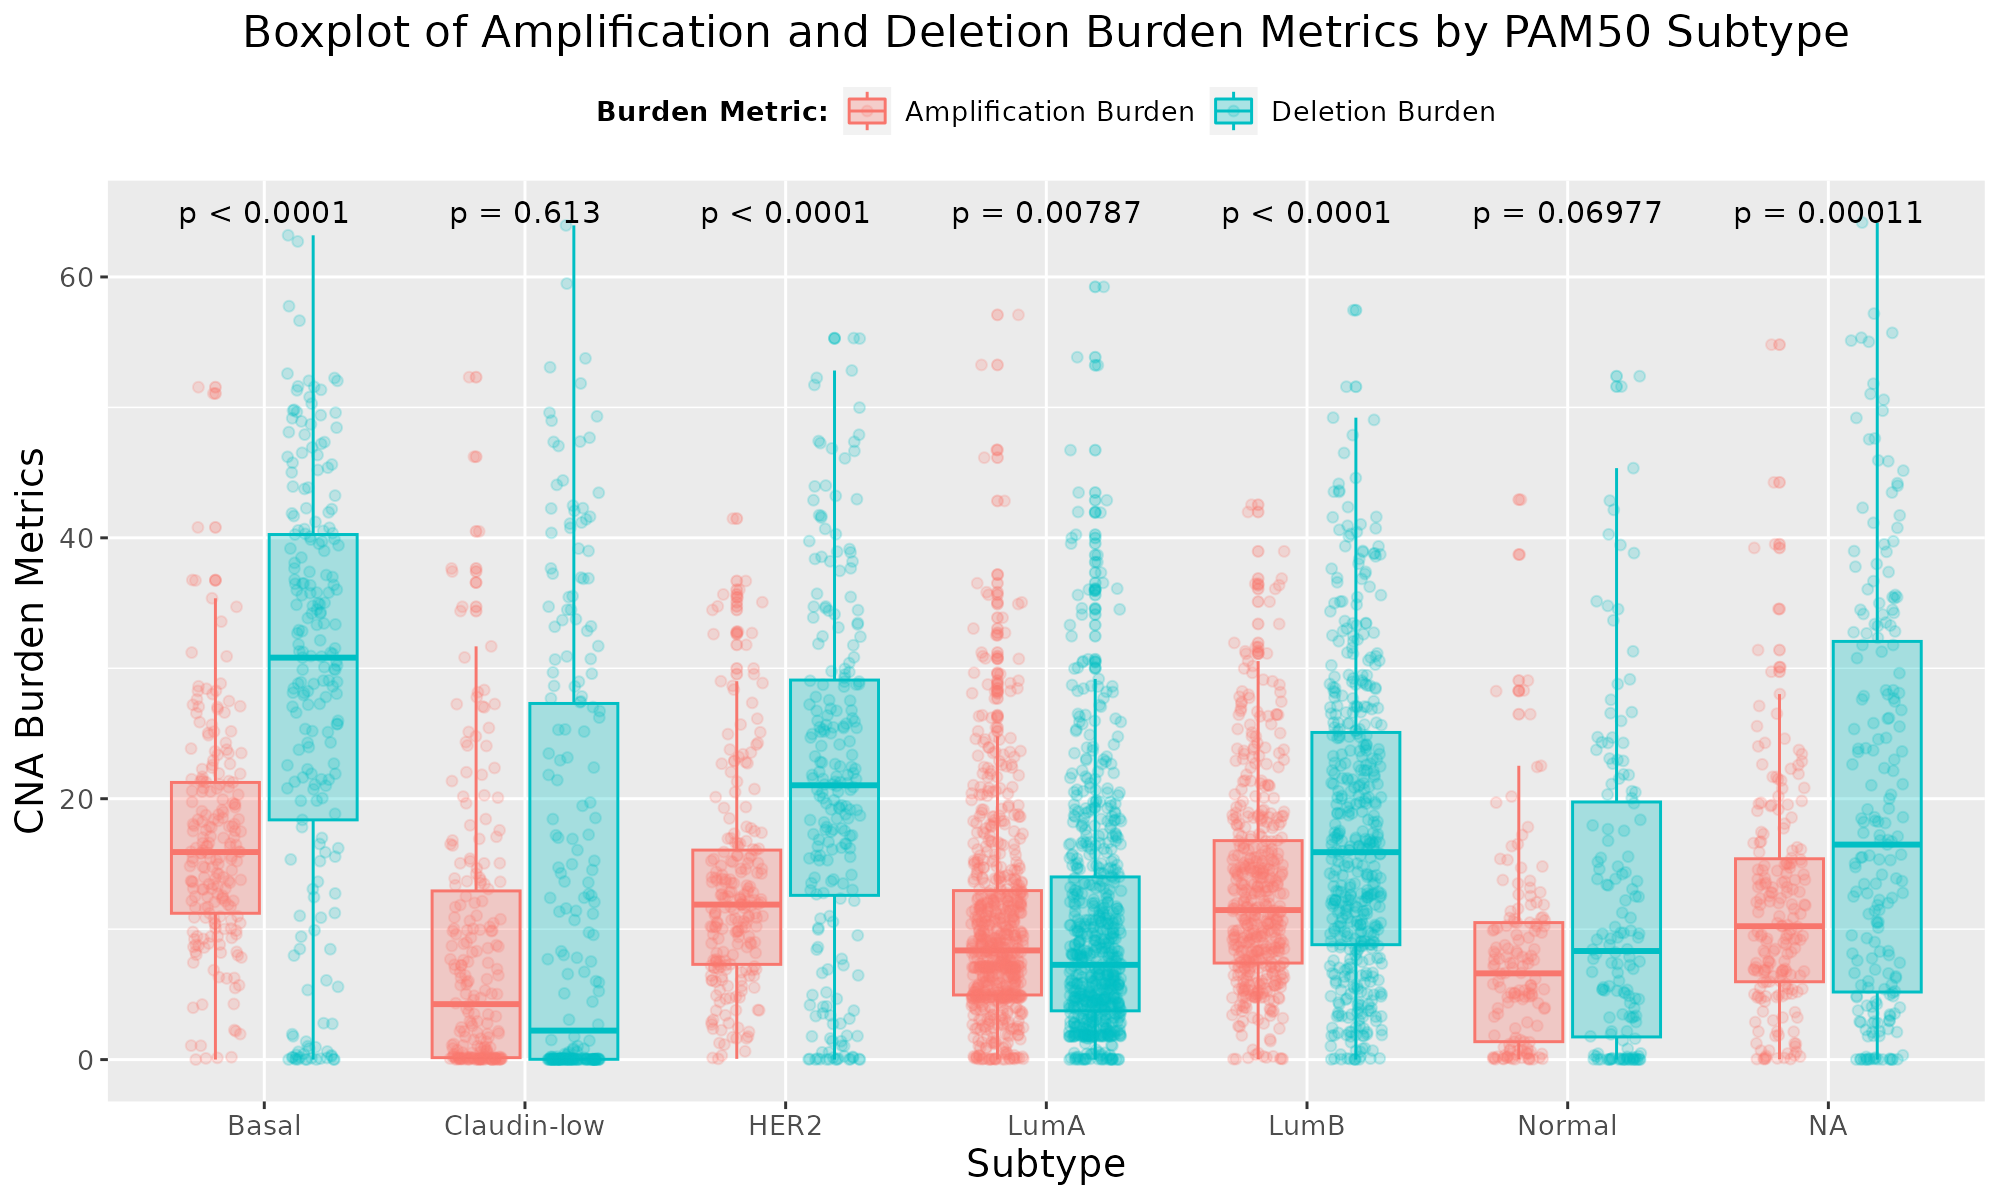
\includegraphics[width=1\textwidth]{../figures/Chapter_2/Global_CNA_Burden_AmpDel_Across_PAM50.png}
\caption[Boxplots for each CNA Amp and CNA Del Burden metric by PAM50 subtype.]{Boxplots for each CNA Amp and CNA Del Burden metric by PAM50 subtype. Includes Benjamini-Hochberg adjusted Kruskal-Wallis p-values.}
\label{fig:CNA-Burden-Metric-Boxplots-P50-AmpDel}
\end{figure}
\clearpage 

The observed distribution of the six CNA metrics, for patients stratified by IntClust is provided (Figures \ref{fig:CNA-Score-Metric-Boxplots-IC} and \ref{fig:CNA-Burden-Metric-Boxplots-IC}), accompanied by BH adjusted Kruskal-Wallis p-values. These figures indicate some significant difference exists comparing each of the CNA metric distributions across IntClusts (Kruskall-Wallis adjusted $p<0.0001$ for all CNA metrics).

\begin{figure}[!ht]
\center
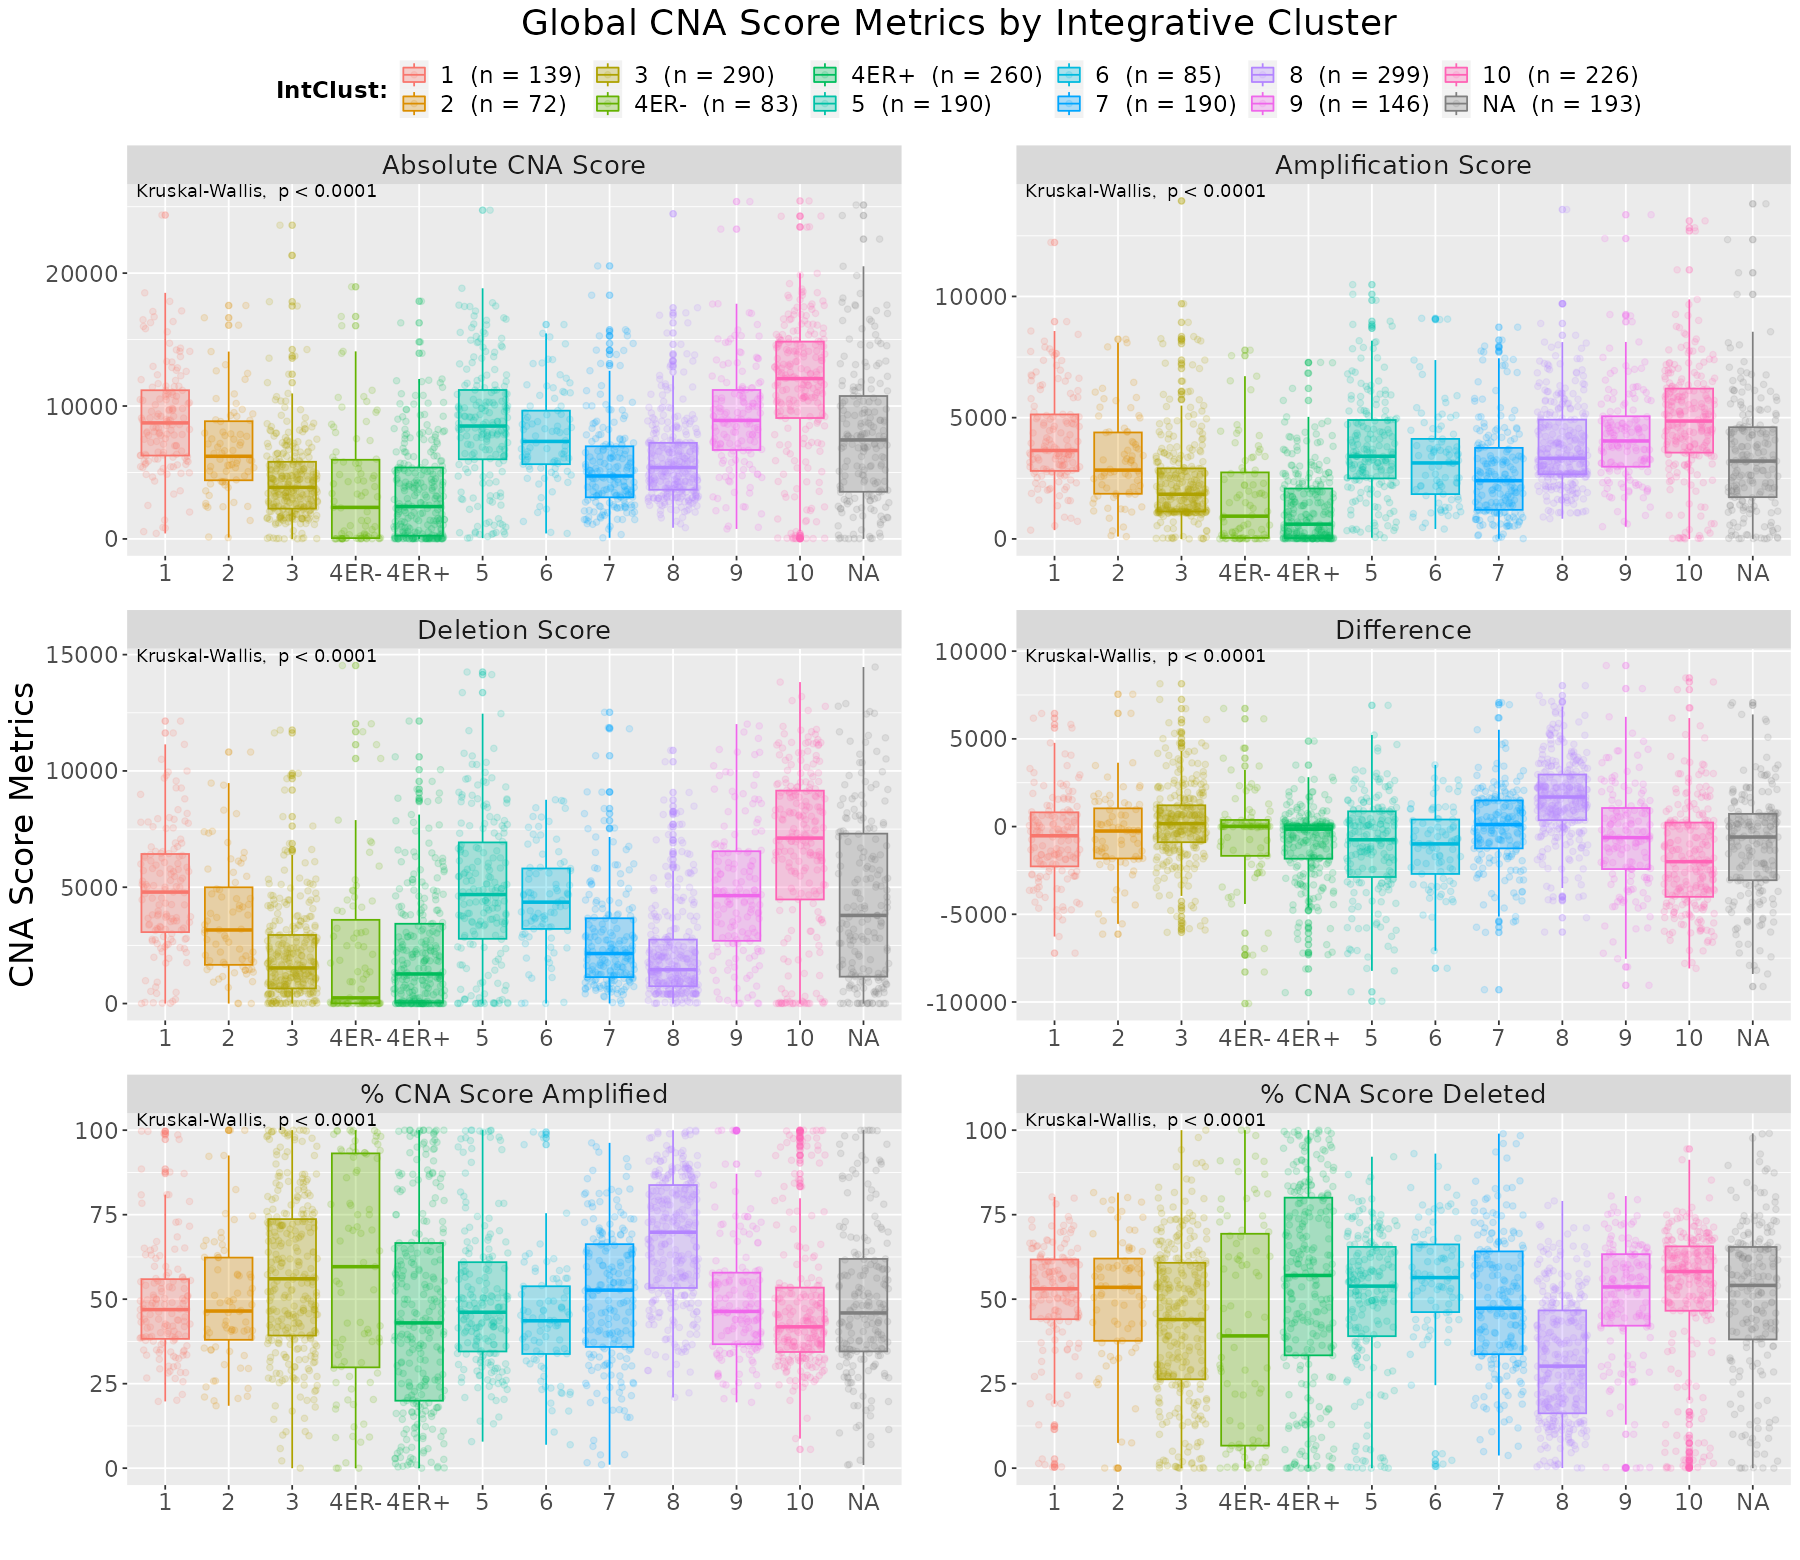
\includegraphics[width=1\textwidth]{../figures/Chapter_2/Global_CNA_Score_Metrics_Across_IntClust.png}
\caption[Boxplots for each CNA Score metric by IntClust.]{Boxplots for each CNA Score metric by IntClust. Each facet contains boxplots for the CNA Score metrics calculated using all available data and Benjamini-Hochberg adjusted Kruskal-Wallis p-values. NA denotes METABRIC patients missing IntClust information.}
\label{fig:CNA-Score-Metric-Boxplots-IC}
\end{figure}

\begin{figure}[!ht]
\center
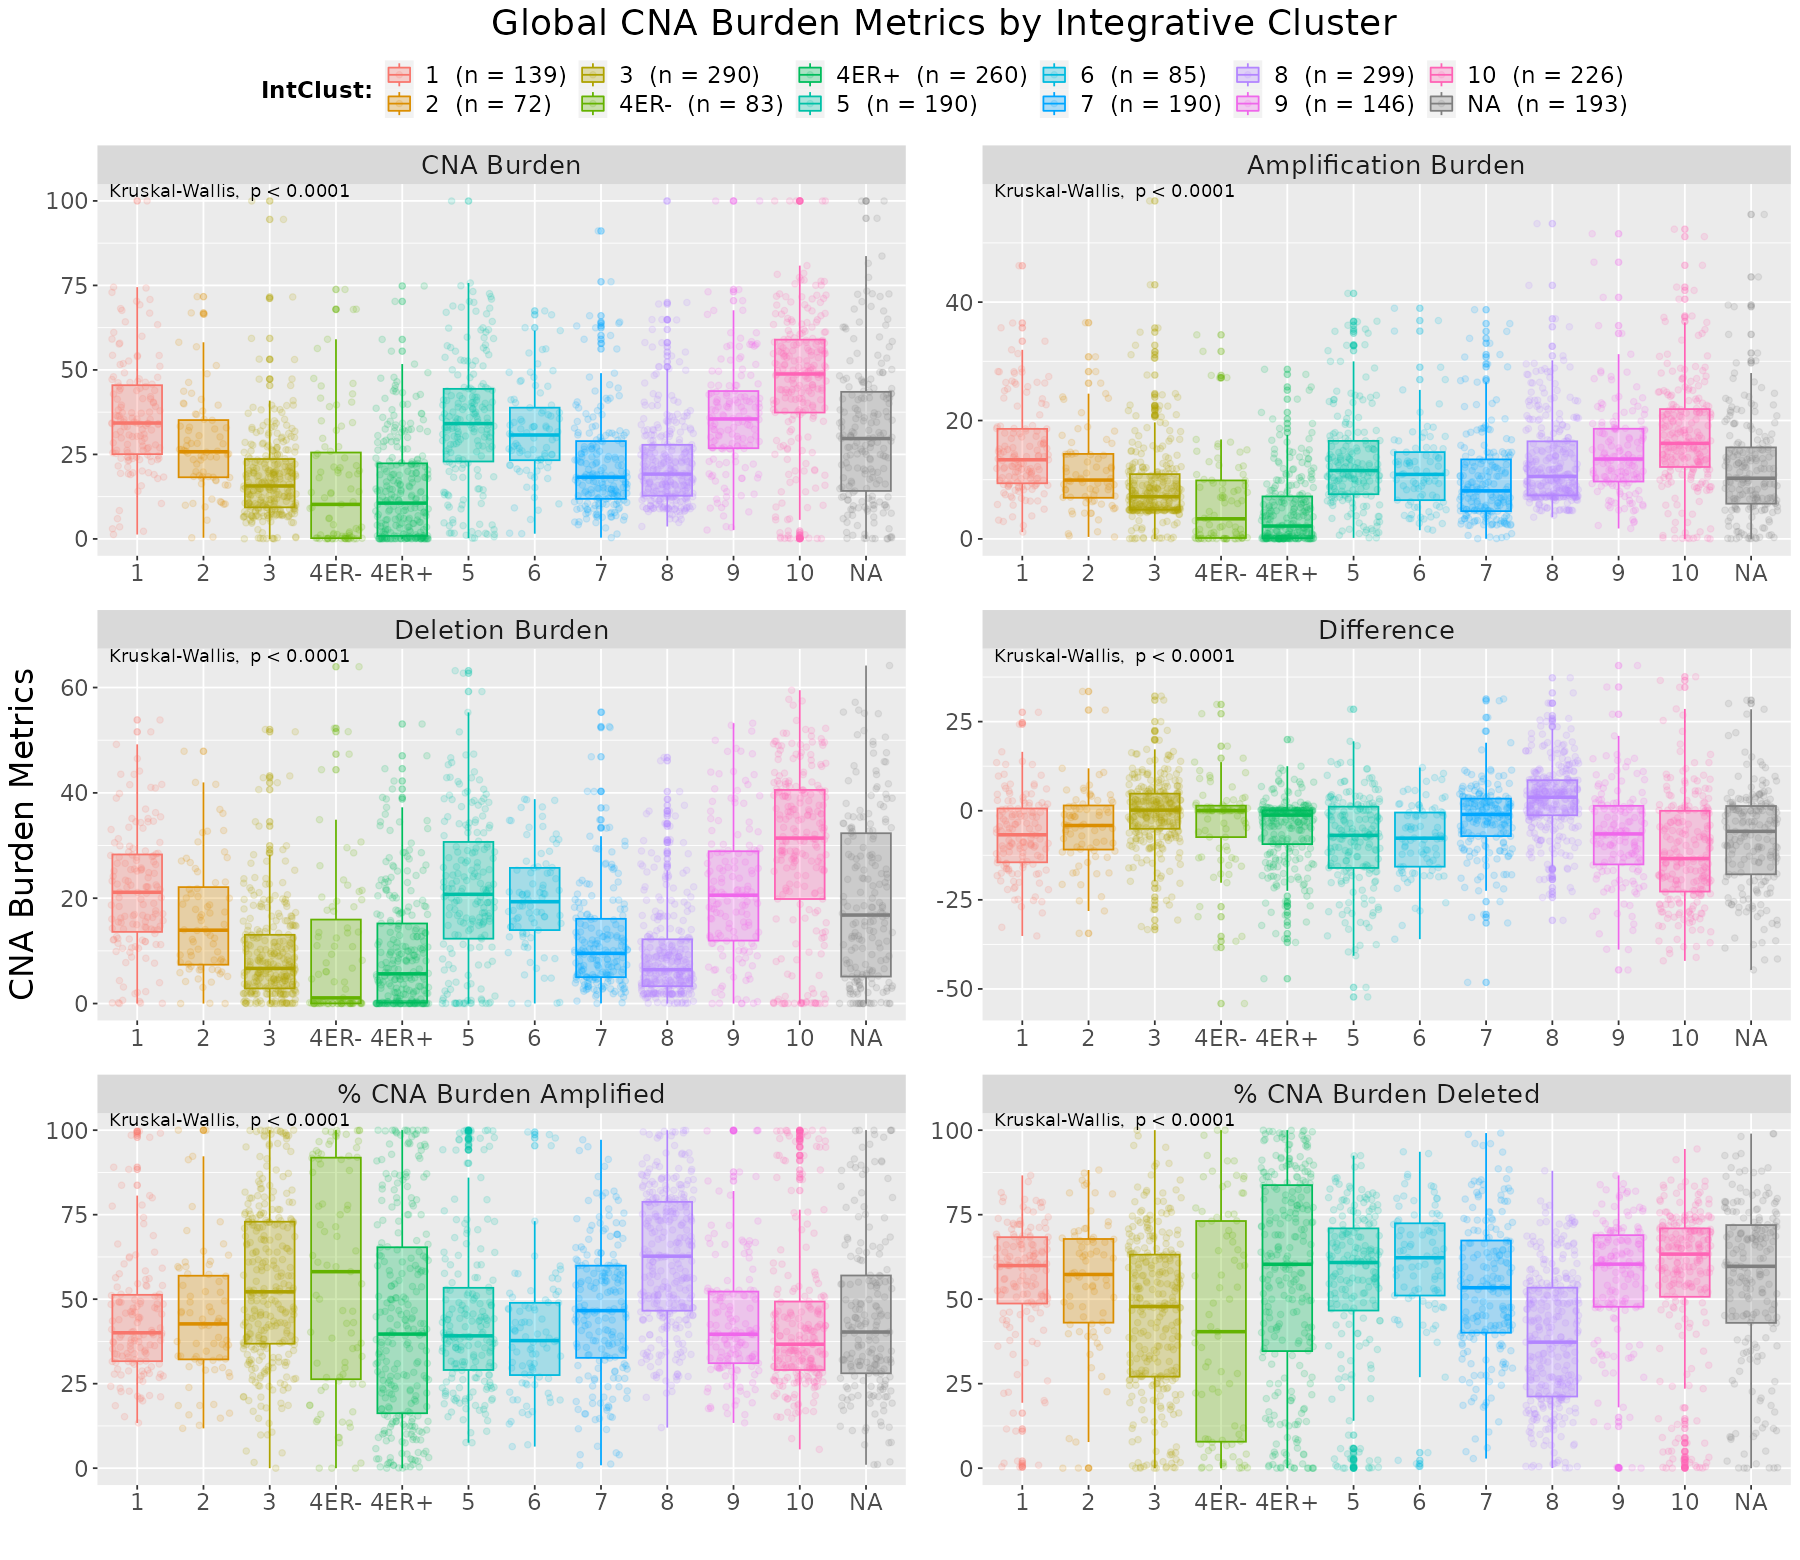
\includegraphics[width=1\textwidth]{../figures/Chapter_2/Global_CNA_Burden_Metrics_Across_IntClust.png}
\caption[Boxplots for each CNA Burden metric by IntClust.]{Boxplots for each CNA Burden metric by IntClust. Each facet contains boxplots for the CNA Burden metrics calculated using all available data and Benjamini-Hochberg adjusted Kruskal-Wallis p-values. NA denotes METABRIC patients missing IntClust information.}
\label{fig:CNA-Burden-Metric-Boxplots-IC}
\end{figure}

IntClust 10 displays the highest absolute, amplification and deletion CNA Score and Burden metrics (Dunn’s test $p < 0.0001$ for most comparisons, Tables \ref{tab:DT_Score_2} and \ref{tab:DT_Burden_2}). This is not surprising as IntClust 10 is primarily made up of Basal patients (Figure \ref{fig:Comp}). IntClust 1, 5 and 9 also display high levels of GI and are primarily composed of the PAM50 subtypes that have higher levels of GI, i.e. Basal, HER2 and Luminal B subtype. The densities of these distributions, apart from the CNA Amp metric distribution, are not significantly different from each other ($p > 0.05$). The levels of amplification burden observed in IntClust 5 are significantly lower than the levels observed in IntClust 1 and 9 ($p = 0.01$ and $p = 0.02$, respectively). IntClust 3, 4ER-, ER+, and 7 are primarily composed of Luminal A, Normal and Claudin-low subtypes (Figure \ref{fig:Comp}). These subtypes display low levels of GI and as such the boxplots display the lowest CNA Score and Burden metrics, except for CNA Del Score and Burden where IntClust 8 displays lower levels of deletions, when compared with IntClust 7. The distributions of IntClust 4ER- and 4ER+ do not significantly differ from each other, while IntClust 3 displays significantly more amplifications than IntClust 4ER+ and 4ER- ($p < 0.0001$ and $p < 0.01$, respectively), and IntClust 7 has significantly higher distributions across all metrics ($p < 0.01$, Tables \ref{tab:DT_Score_2} and \ref{tab:DT_Burden_2}).

Focusing on the direct comparison of levels of amplification to deletion within each IntClust, Figures \ref{fig:CNA-Score-Metric-Boxplots-IC-AmpDel} and \ref{fig:CNA-Burden-Metric-Boxplots-IC-AmpDel}, IntClust 2, 5 and 10, three clusters associated with poorer survival outcome, have significantly higher levels of deletions than amplifications ($p = 0.034$, $p < 0.0001$ and $p < 0.0001$, respectively). IntClust 1, 4ER+ and 6 also display significantly more deletions than amplifications but correspond to intermediate or good survival outcome ($p < 0.0001$, $p = 0.0005$ and $p < 0.0001$, respectively). The remaining IntClust classifications observed by \cite{pmid22522925} to have favourable survival outcomes, i.e. IntClust 3, 4ER-, 7 and 8, show no significant difference in the levels of amplifications and deletions, IntClust 3, 4ER-, 7 ($p > 0.05$) or significantly more amplifications than deletions, IntClust 8 ($p < 0.0001$).

\begin{table}[!ht]
\caption[Comparisons of CNA Score metric distributions by Integrative Cluster.]{Comparisons of CNA Score metric distributions by Integrative Cluster. Z statistics and Benjamini-Hochberg adjusted p-values for each Dunn's test are shown.}
\begin{minipage}[c]{0.45\textwidth}
\centering
\begin{tabular}{ccc}
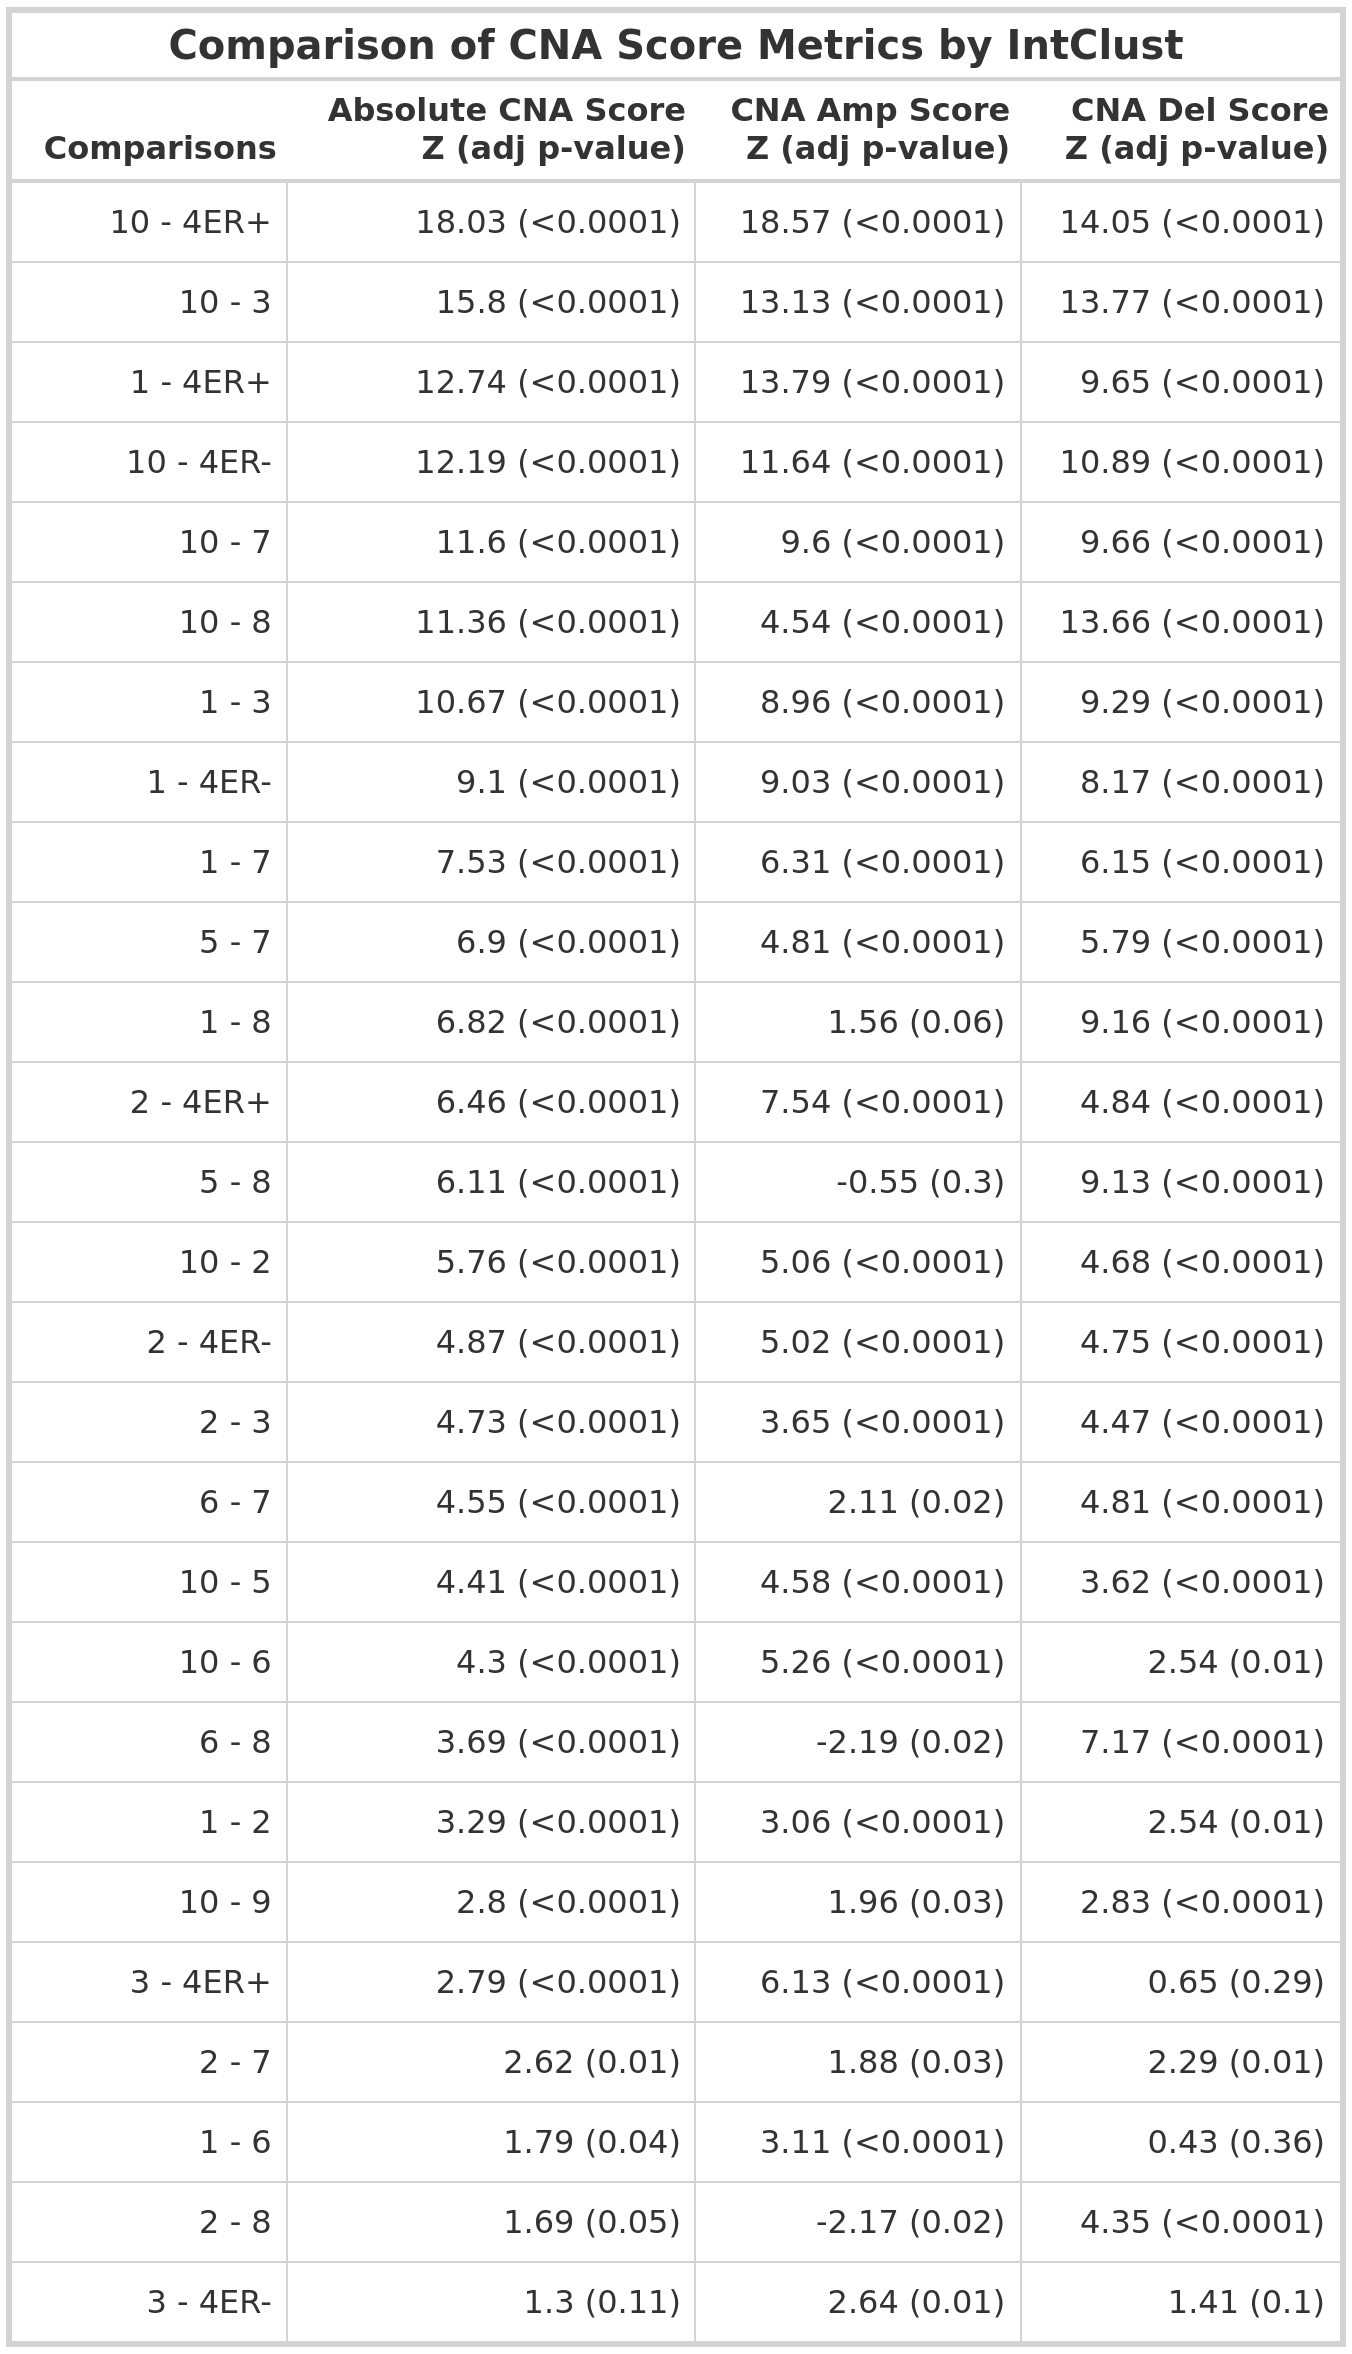
\includegraphics[width=0.98\textwidth]{../tables/Chapter_2/Global_CNA_Score_Metric_IntClust_Comparisons_1.png}
\end{tabular}
\end{minipage}
\hspace{0.8cm}
\begin{minipage}[c]{0.45\textwidth}
\centering
\begin{tabular}{ccc}
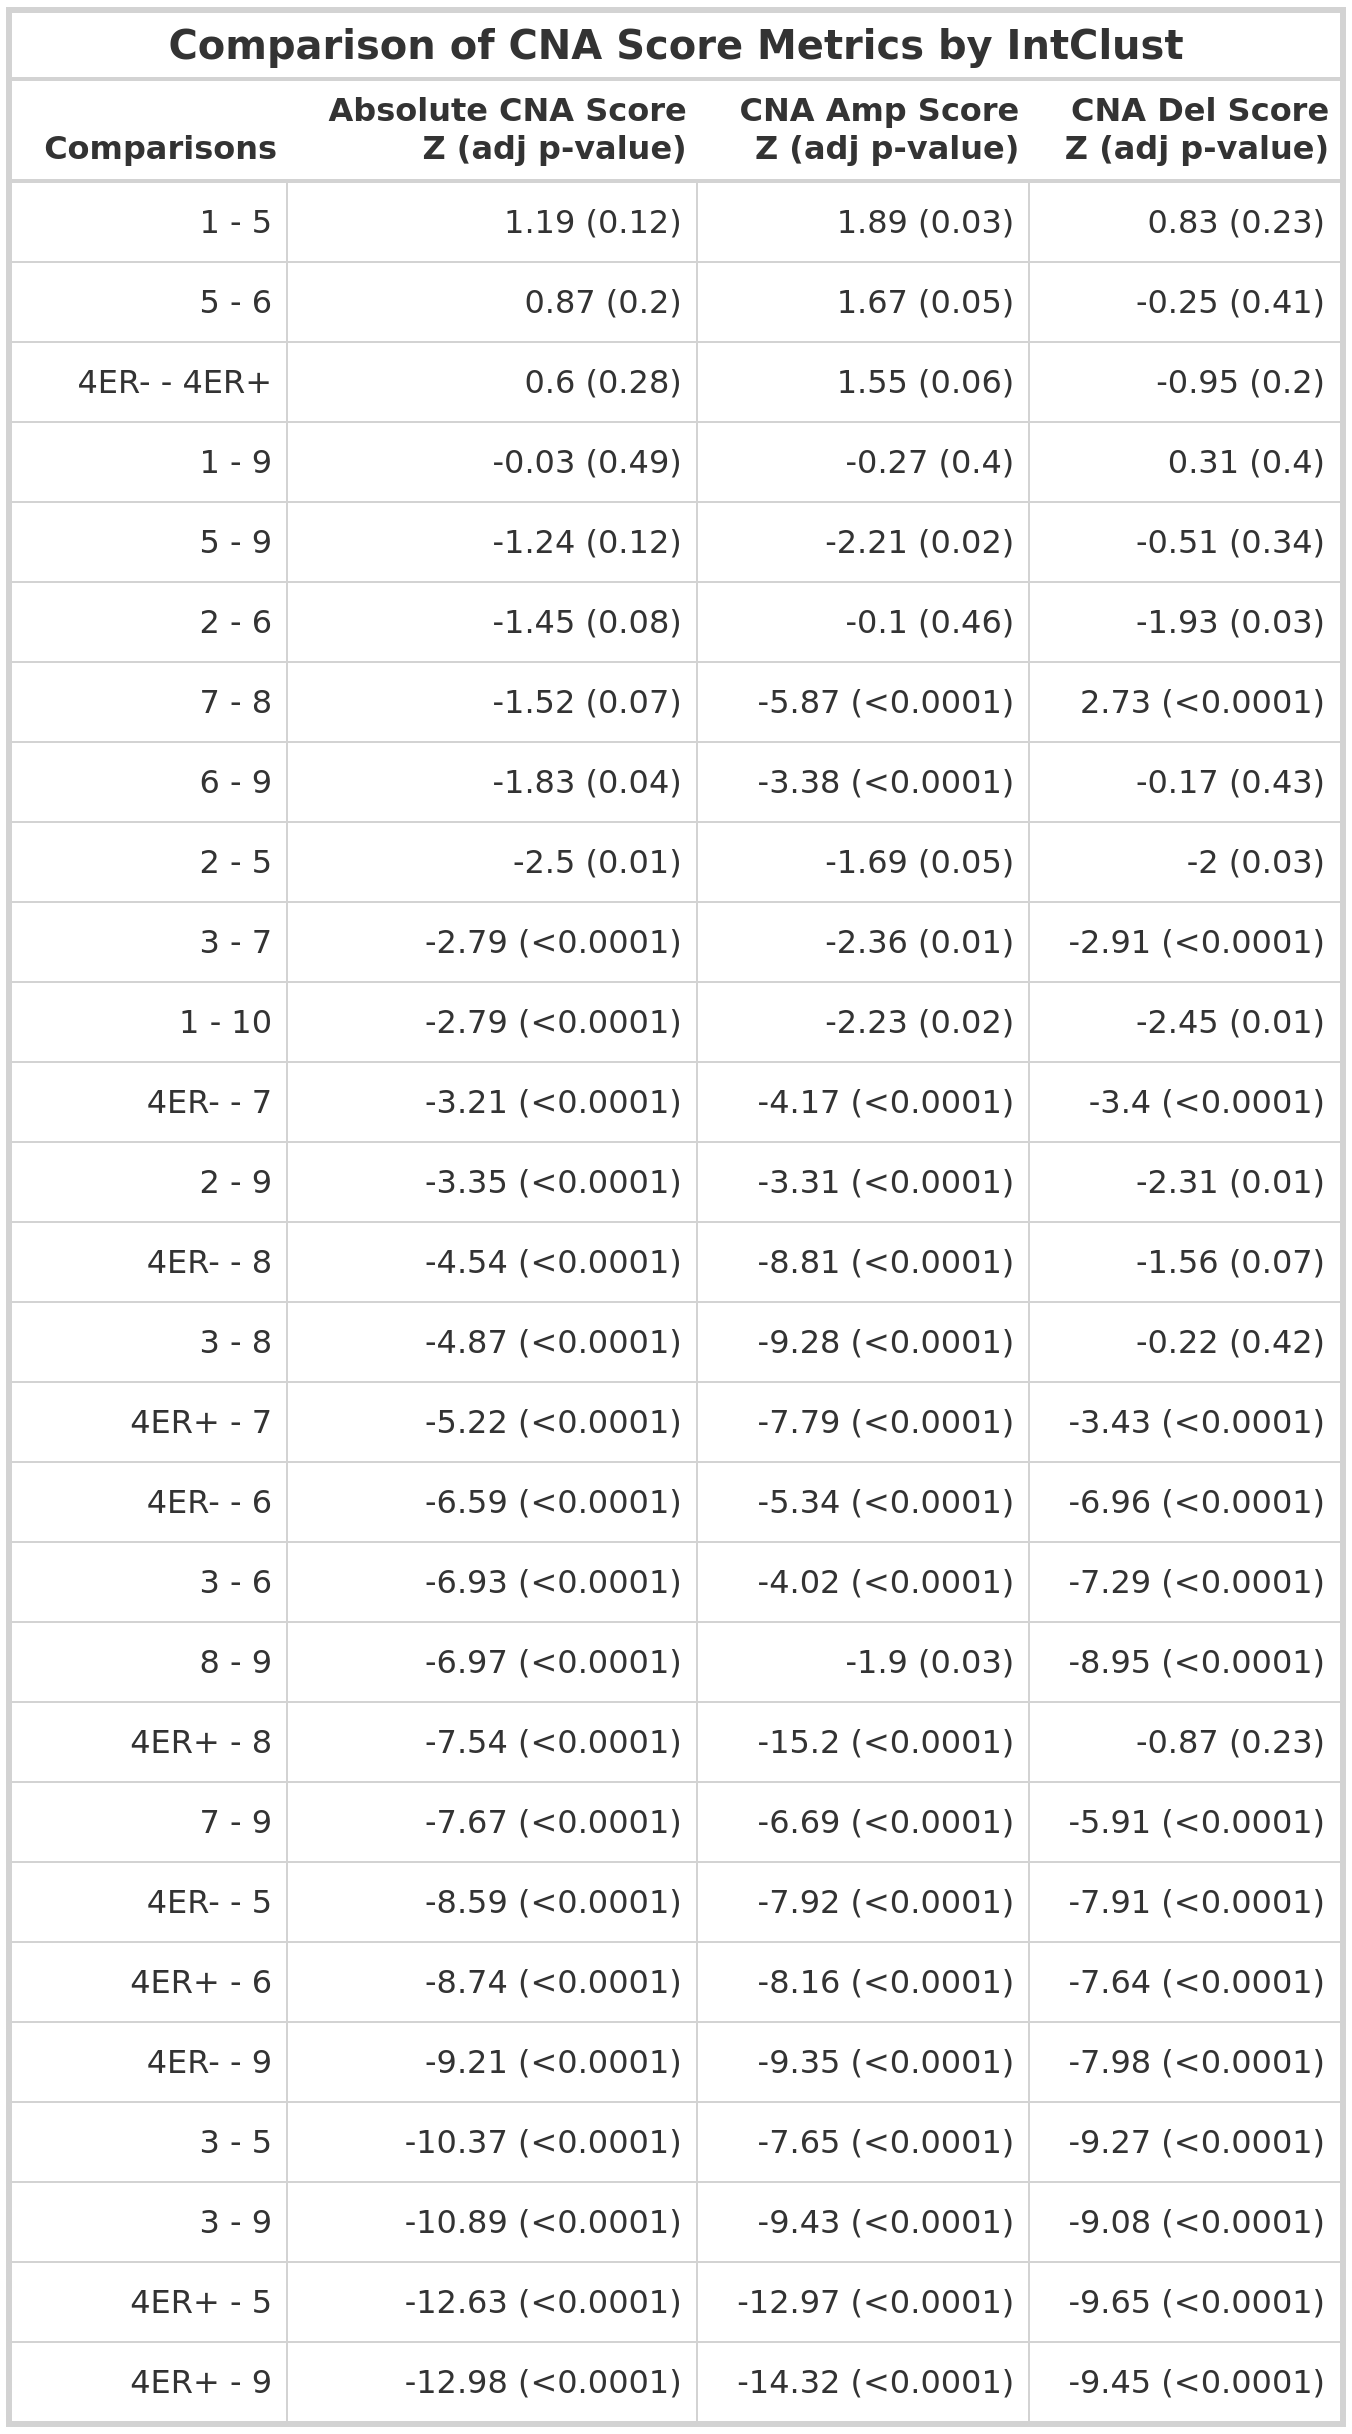
\includegraphics[width=0.96\textwidth]{../tables/Chapter_2/Global_CNA_Score_Metric_IntClust_Comparisons_2.png}
\end{tabular}
\end{minipage}
\label{tab:DT_Score_2}
\end{table}

\begin{figure}[!ht]
\center
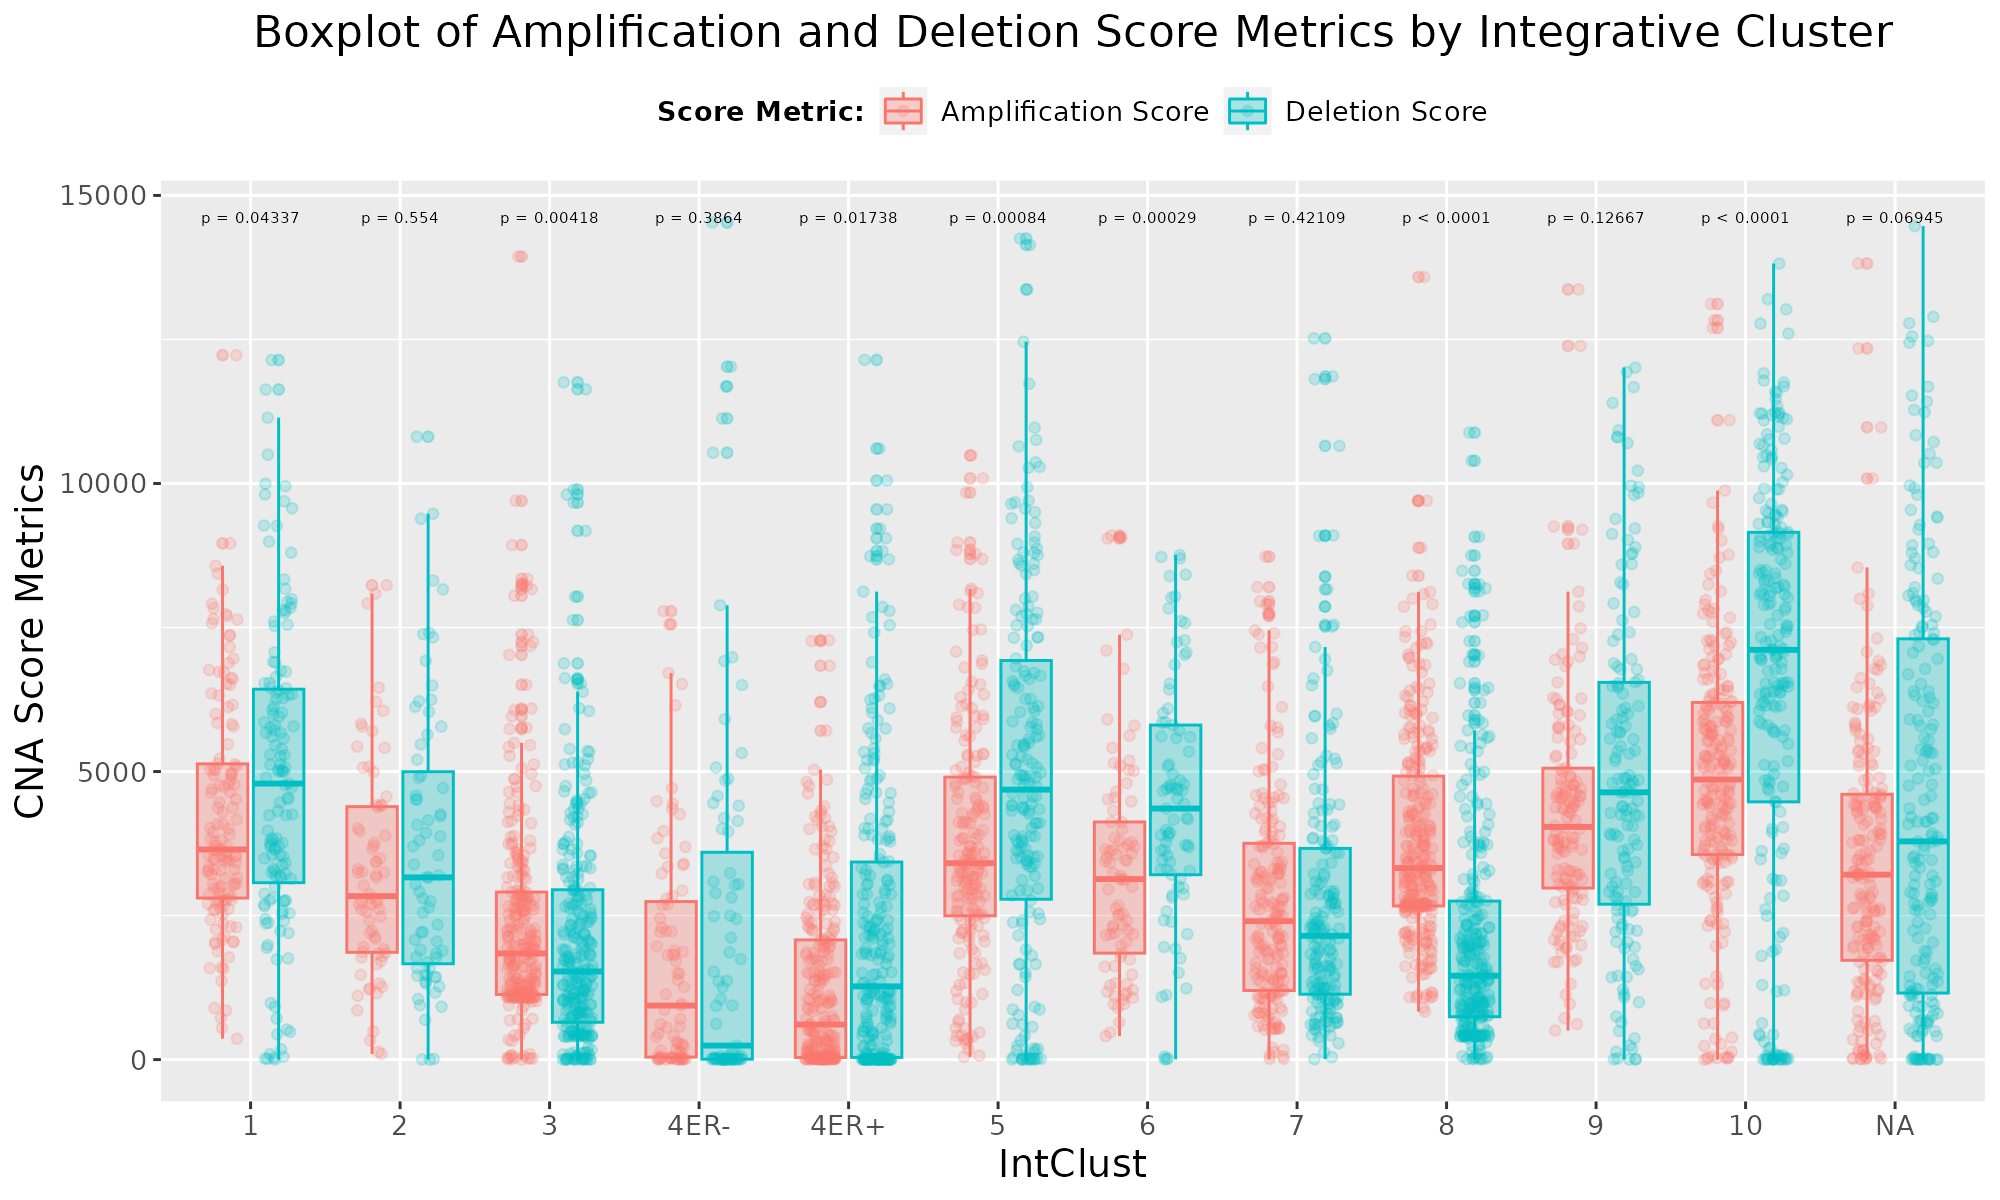
\includegraphics[width=0.97\textwidth]{../figures/Chapter_2/Global_CNA_Score_AmpDel_Across_IC.png}
\caption[Boxplots for each CNA Amp and CNA Del Score metric by Integrative Cluster.]{Boxplots for each CNA Amp and CNA Del Score metric by Integrative Cluster. Includes Benjamini-Hochberg adjusted Kruskal-Wallis p-values.}
\label{fig:CNA-Score-Metric-Boxplots-IC-AmpDel}
\end{figure}

\begin{table}[!ht]
\caption[Comparisons of CNA Burden metric distributions by Integrative Cluster.]{Comparisons of CNA Burden metric distributions by Integrative Cluster. Z statistics and Benjamini-Hochberg adjusted p-values for each Dunn's test are shown.}
\begin{minipage}[c]{0.45\textwidth}
\centering
\begin{tabular}{ccc}
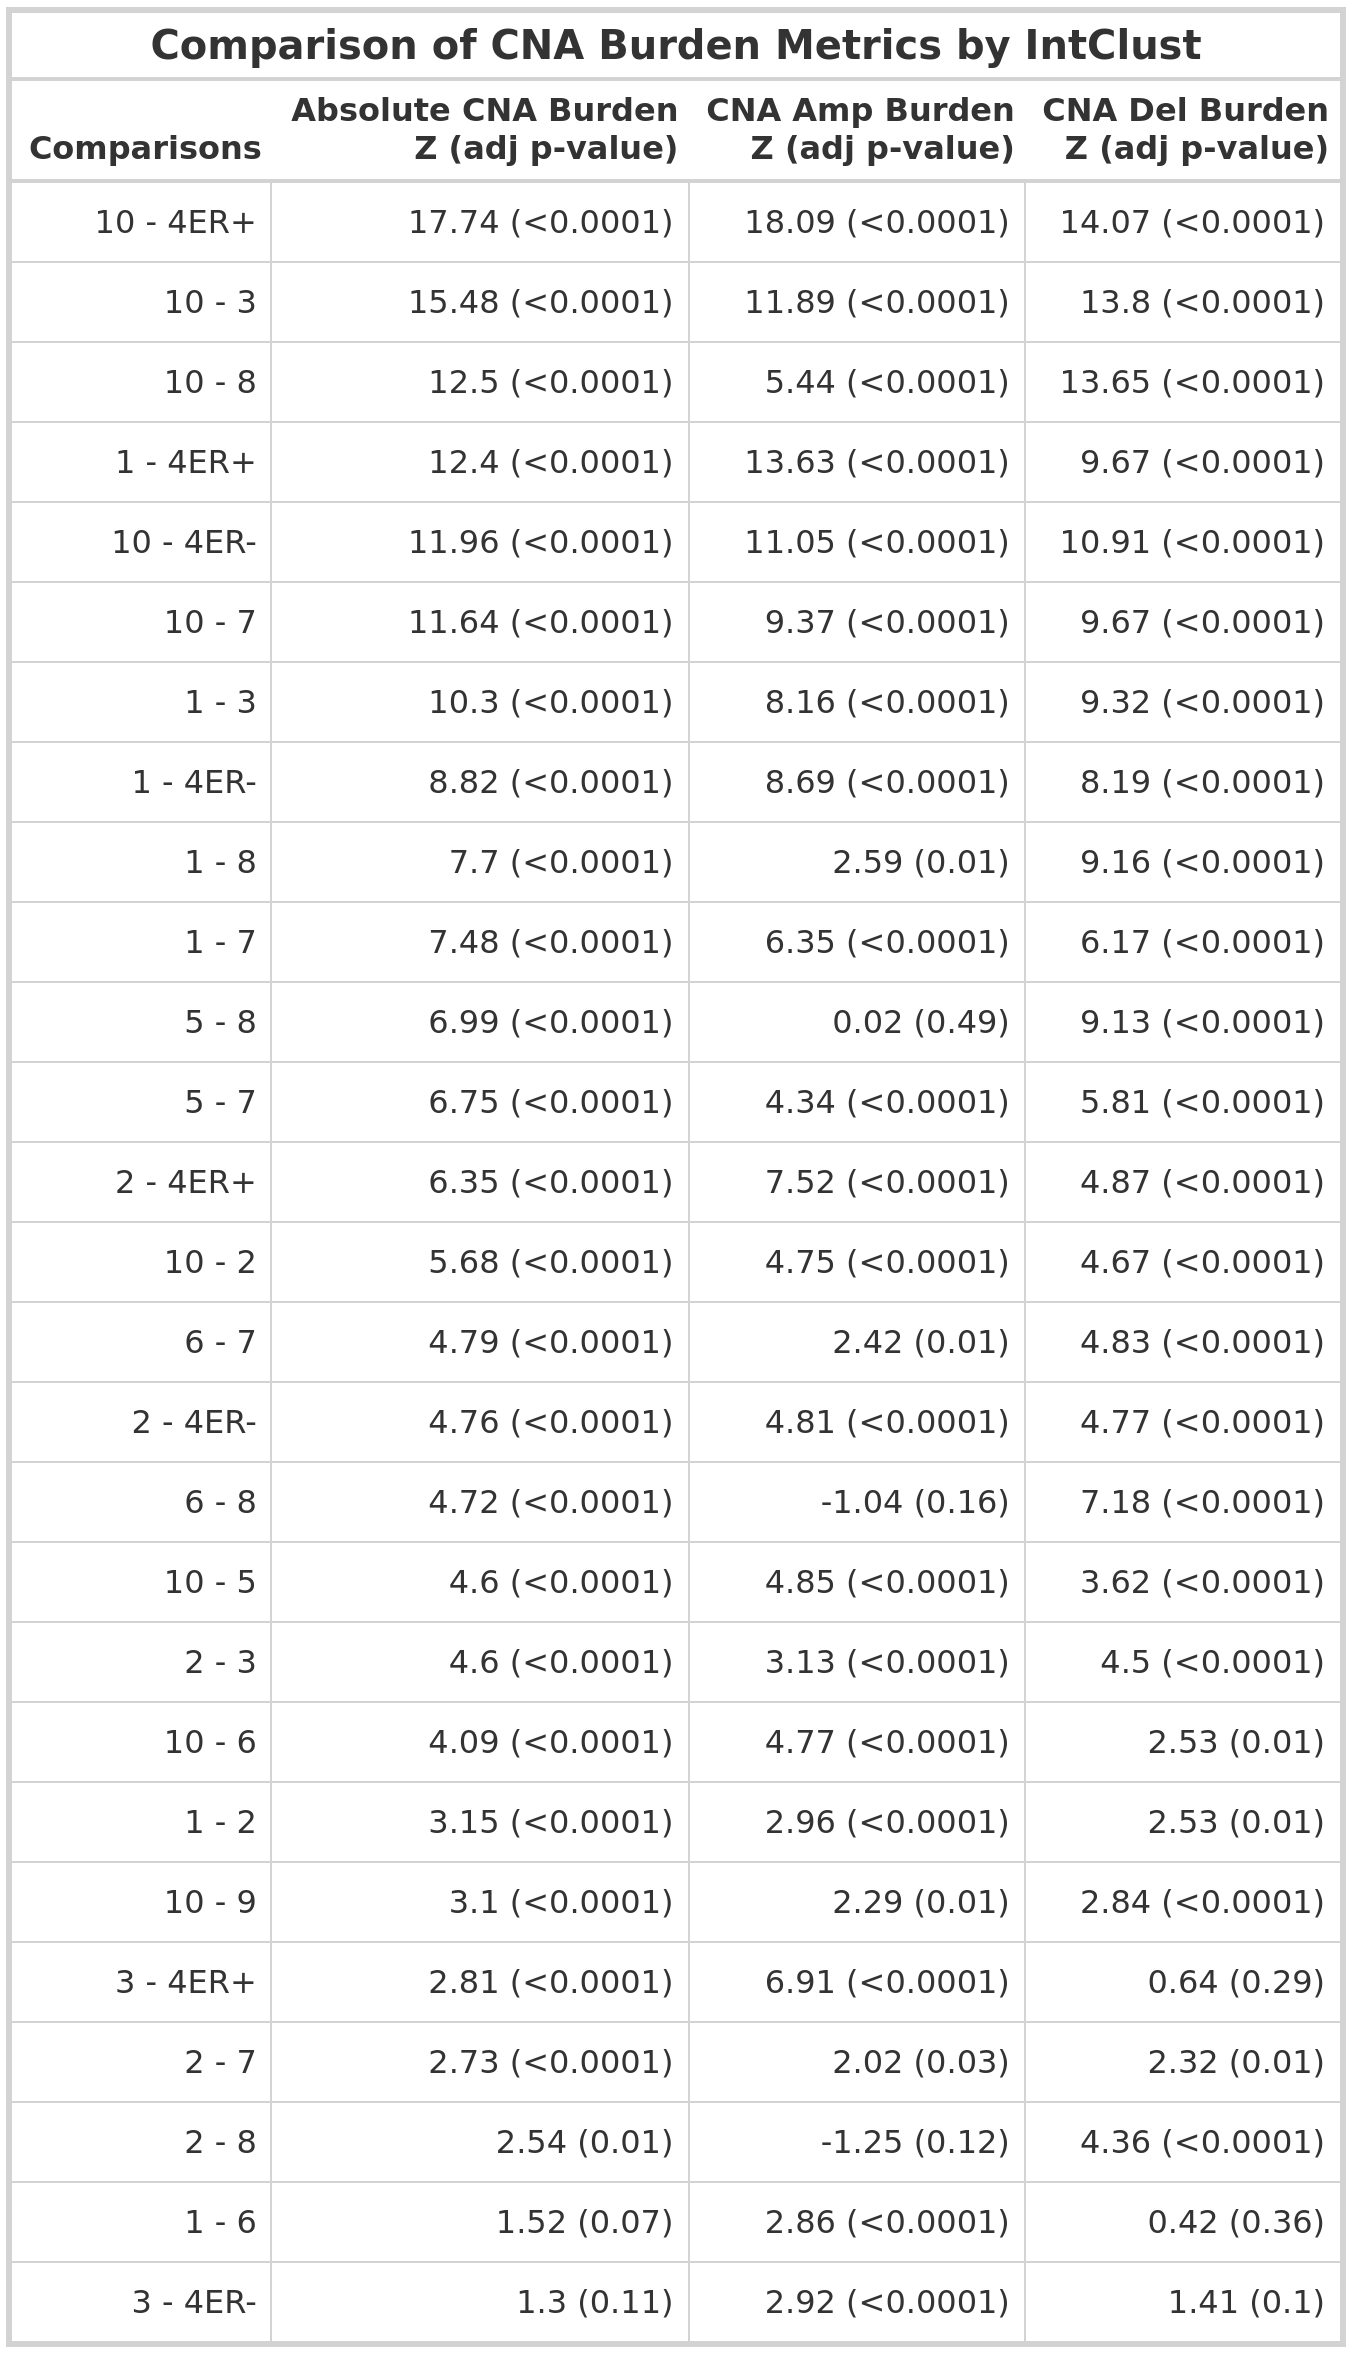
\includegraphics[width=0.98\textwidth]{../tables/Chapter_2/Global_CNA_Burden_Metric_IntClust_Comparisons_1.png}
\end{tabular}
\end{minipage}
\hspace{0.8cm}
\begin{minipage}[c]{0.45\textwidth}
\centering
\begin{tabular}{ccc}
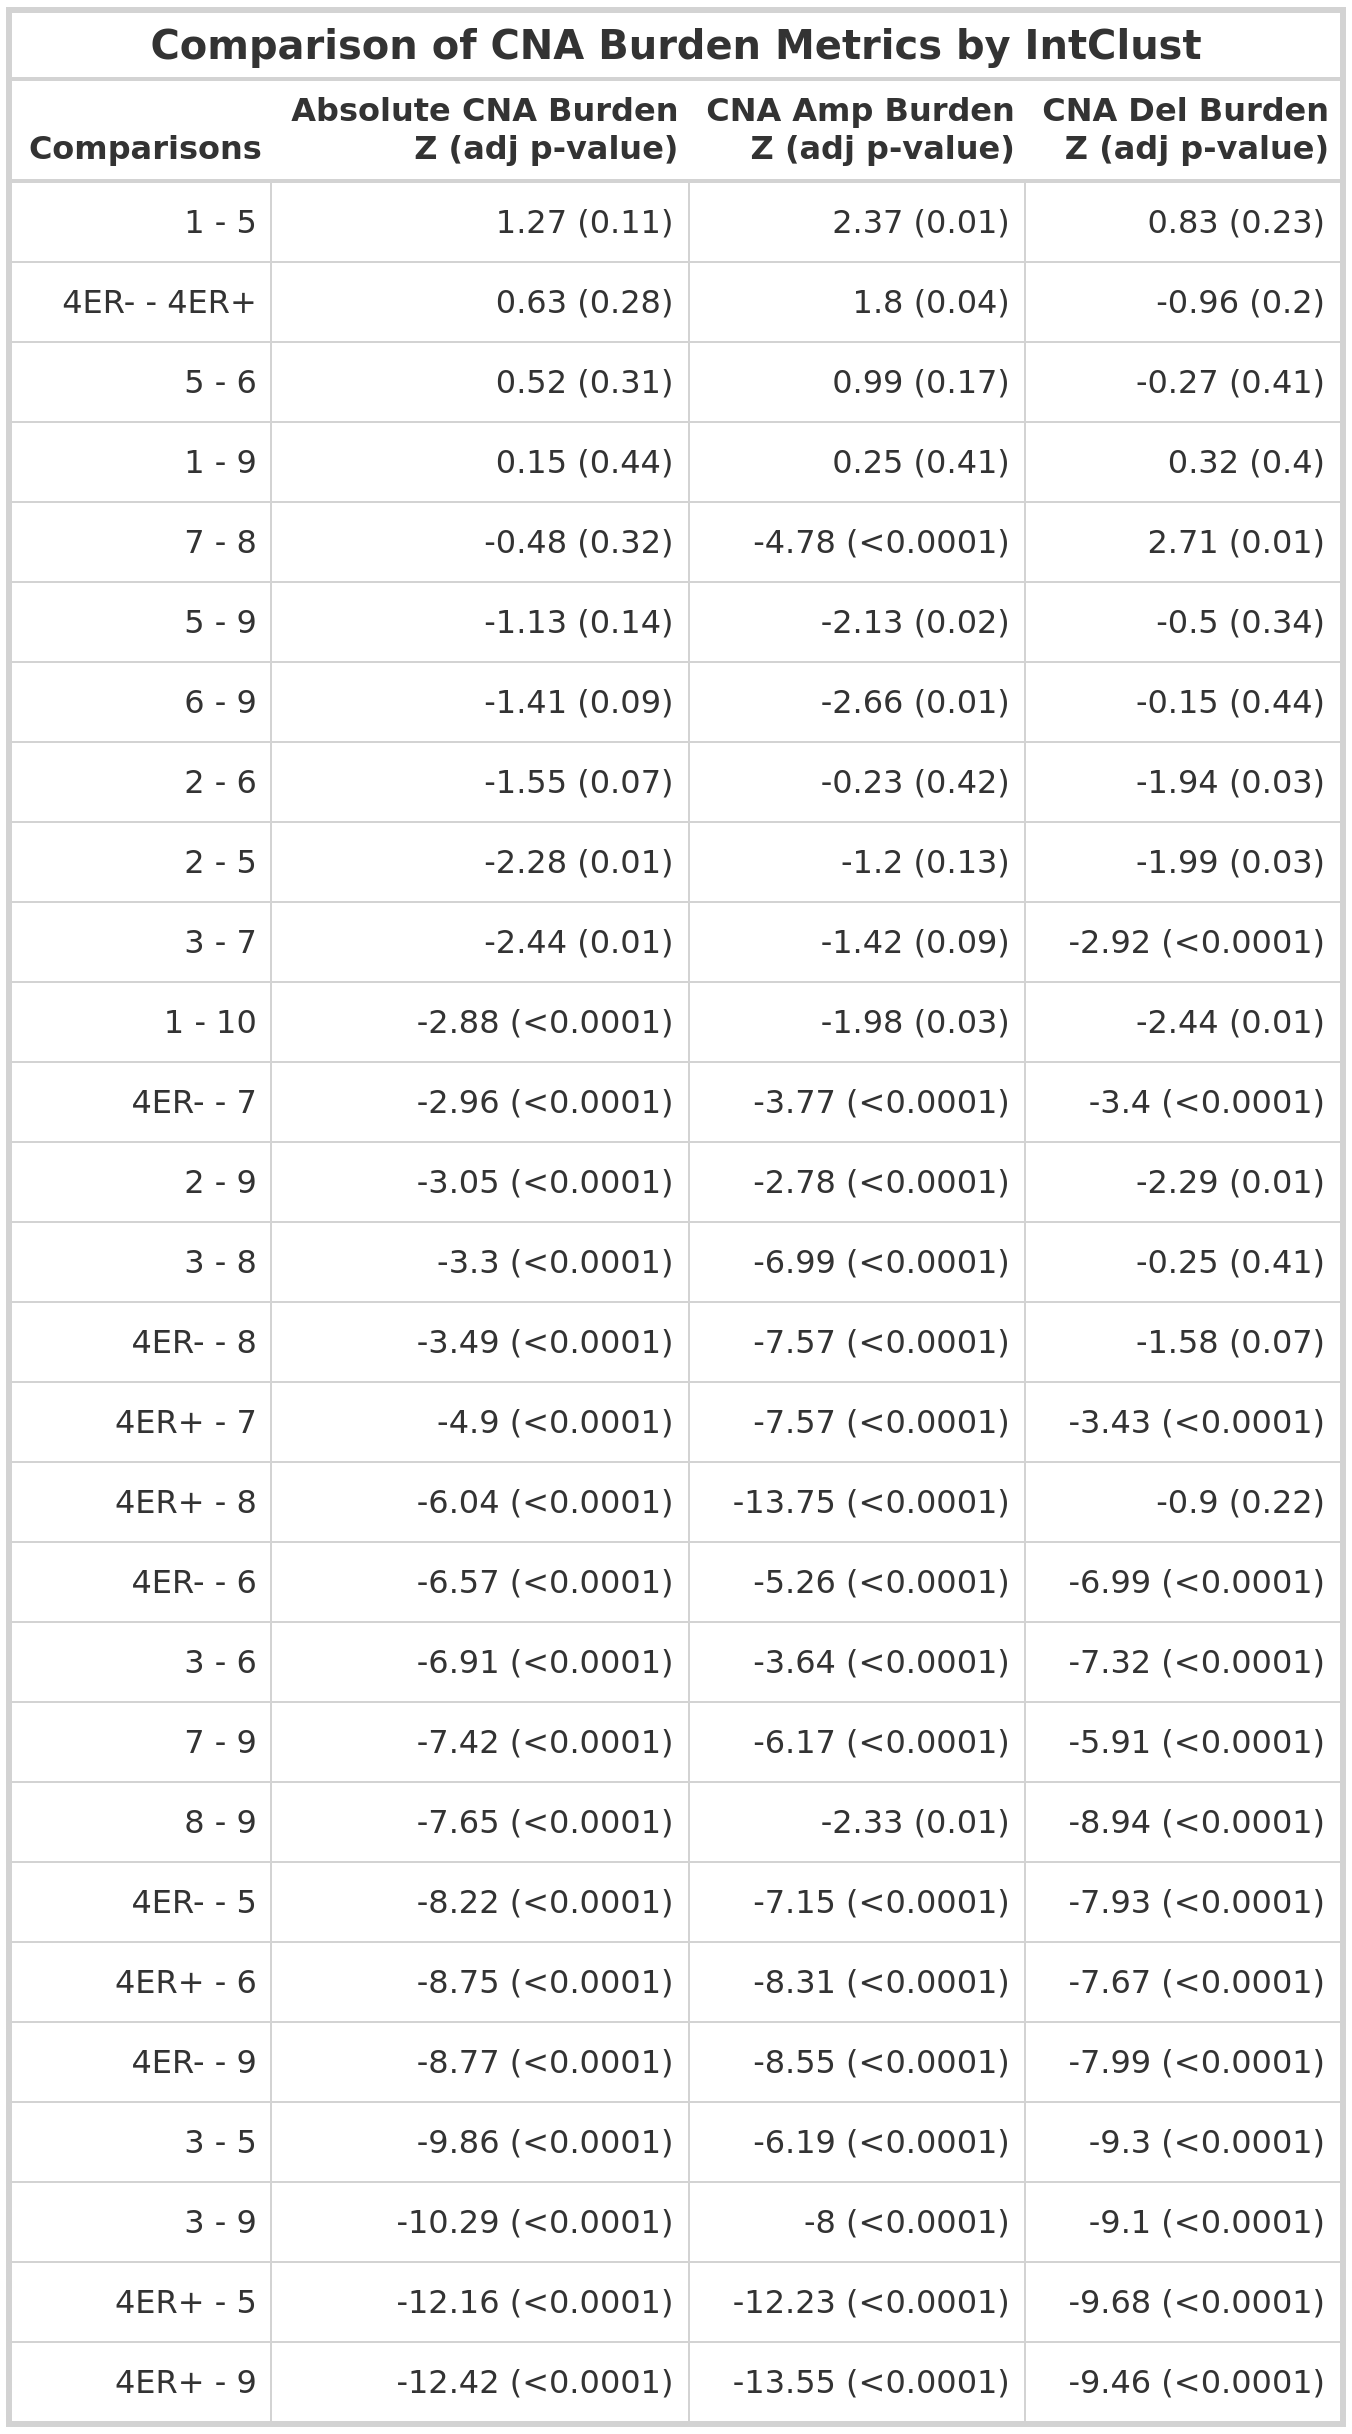
\includegraphics[width=0.96\textwidth]{../tables/Chapter_2/Global_CNA_Burden_Metric_IntClust_Comparisons_2.png}
\end{tabular}
\end{minipage}
\label{tab:DT_Burden_2}
\end{table}

\begin{figure}[!ht]
\center
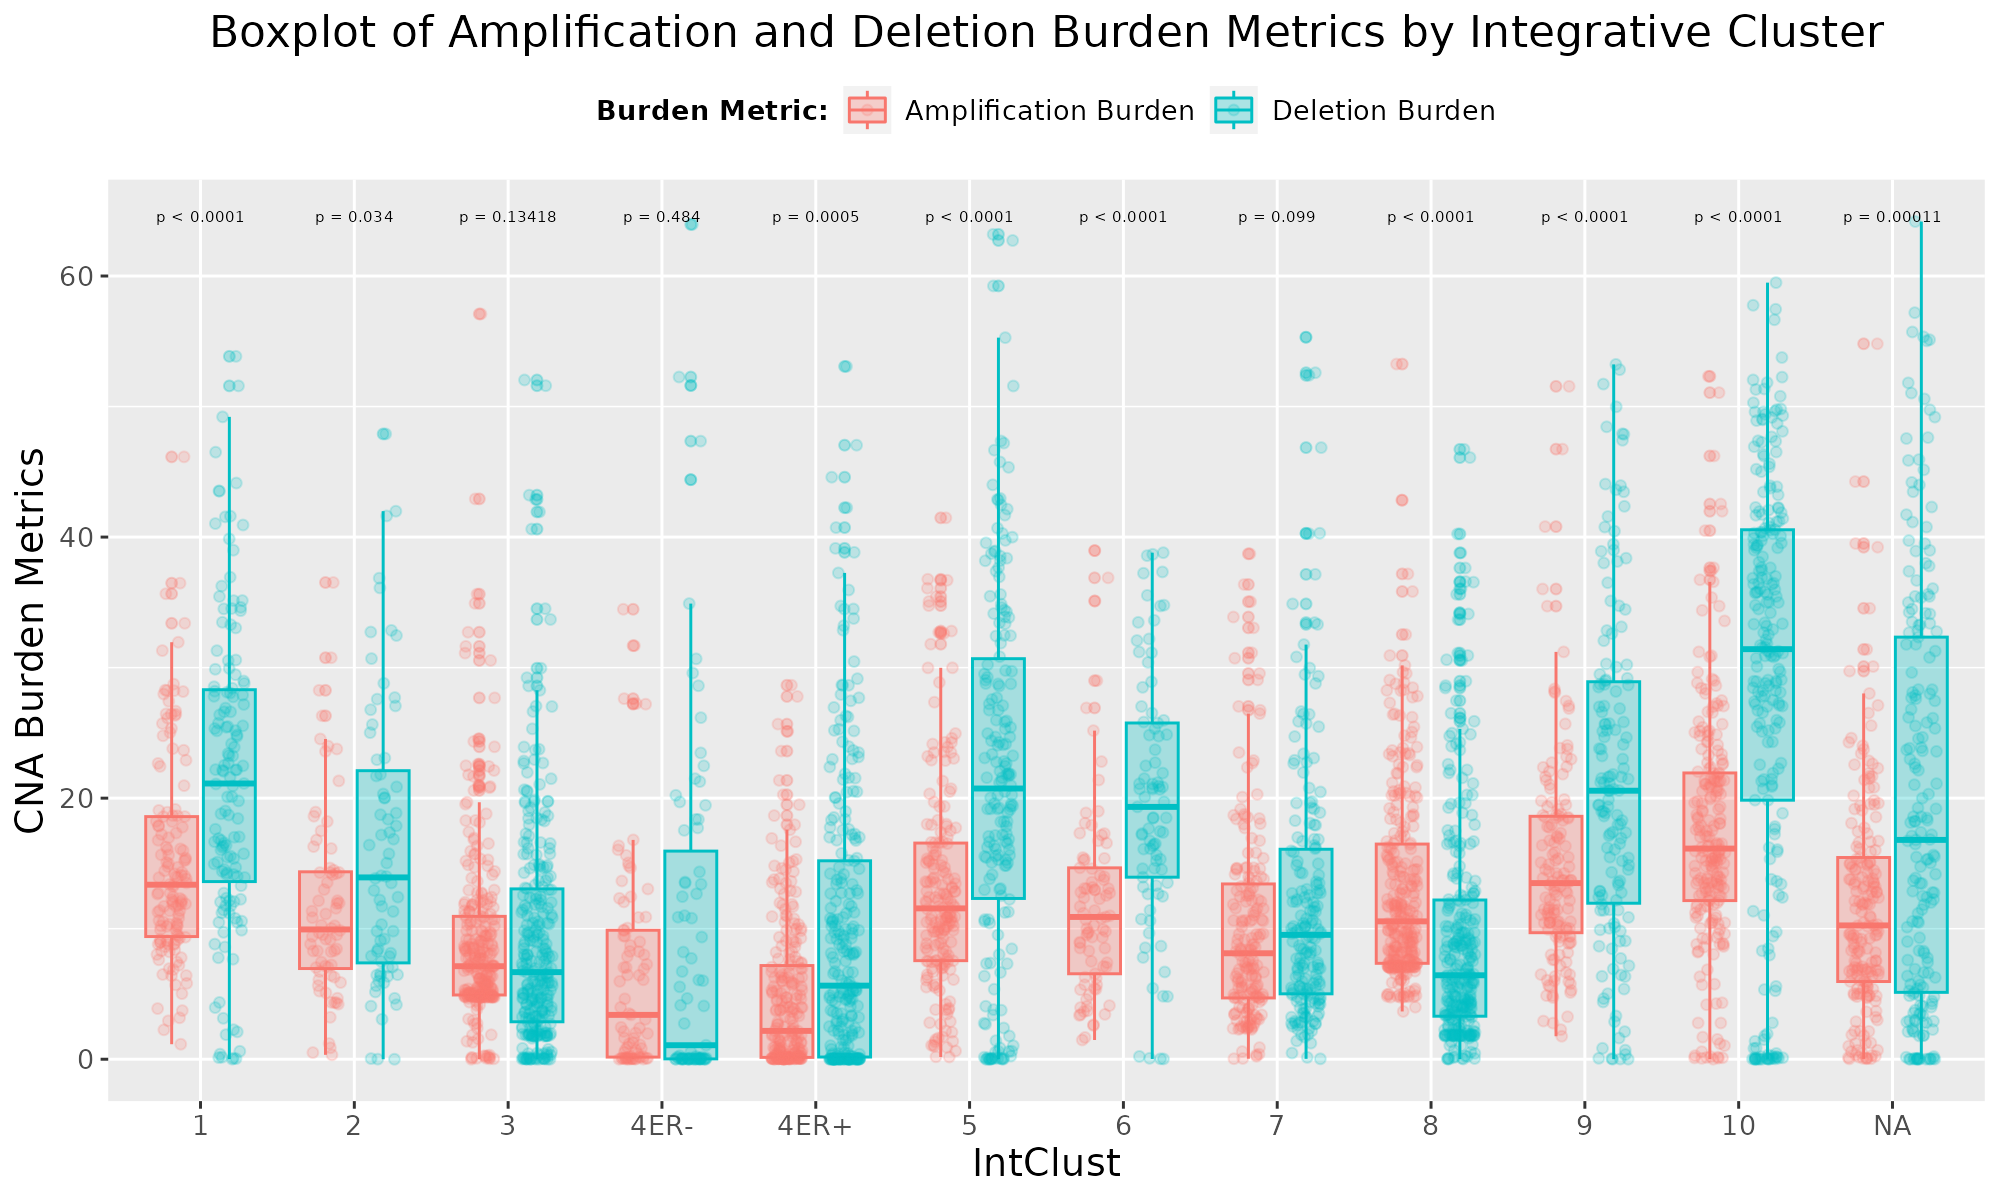
\includegraphics[width=0.97\textwidth]{../figures/Chapter_2/Global_CNA_Burden_AmpDel_Across_IC.png}
\caption[Boxplots for each CNA Amp and CNA Del Burden metric by Integrative Cluster.]{Boxplots for each CNA Amp and CNA Del Burden metric by Integrative Cluster. Includes Benjamini-Hochberg adjusted Kruskal-Wallis p-values.}
\label{fig:CNA-Burden-Metric-Boxplots-IC-AmpDel}
\end{figure}
\clearpage 

\subsubsection{Observed Distributions for Chromosome Arm CNA Metrics across Molecular Subtype Classifications}
\label{ObsDis1}
A similar association analysis is conducted for the 42 chromosome arm CNA Score and Burden metrics. In general, we observe similar effects comparing stratified subgroups of patients in the chromosome arm metrics as observed in the global metrics. 

Although Basal patients displayed widespread GI, some noteworthy alterations primarily observed in Basal patients include high levels of amplifications on chromosome 3q and 10p and deletions on chromosome 3p, 4p, 5q and 15q (Figure \ref{fig:PA-CNA-Score-Metric-Density-P50-5q}). Figure \ref{fig:PA-CNA-Score-Metric-Density-P50-5q} indicates that some significant difference exists comparing each of the selected CNA Burden metric distributions across PAM50 subtype ($p<0.0001$). Applying Dunn's Test to each CNA Burden metric indicates Basal patients display the highest CNA Burden metric across all subtypes, with $p<0.0001$ for all selected CNA metrics and comparisons, indicating higher levels of GI on the specified chromosome arms when compared to other PAM50 subtypes (Table \ref{tab:PA-CNA-Score-Metric-Density-P50-5q}). The highlighted chromosome arms correspond largely to those frequently altered in tumours displaying the “complex I” pattern, which are usually Basal tumours, observed in \cite{pmid17142309}.

Noteworthy alterations observed in HER2 patients include high levels of amplification on chromosome 1q, 8q and 17q, where the HER2 gene is located, and high levels of deletions on chromosome 8p, 17p and 17q (Figure \ref{fig:PA-CNA-Score-Metric-Density-P50-17q}). For each selected CNA Burden metric some significant difference exists comparing each of the CNA metric distributions across PAM50 subtype ($p<0.0001$). Performing pairwise comparisons indicates that HER2 patients display higher CNA Burden metric, across the majority of selected CNA Burden metrics and PAM50 subtypes ($p<0.0001$) except when comparing to Basal patients (Table \ref{tab:PA-CNA-Score-Metric-Density-P50-5q} and \ref{tab:PA-CNA-Score-Metric-Density-P50-17q}). The distributions of the selected CNA Burden metrics in the HER2 and Basal subtypes do not significantly differ from each other ($p>0.05$) indicating similar levels of GI. Exceptions include CNA Amp Burden on chromosome 1q and CNA Amp Burden on chromosome 17q, where HER2 patients display lower and higher levels of amplifications, respectively, when compared with Basal patients ($p = 0.04$ and  $p<0.0001$). Interestingly high levels of deletions are also observed on chromosome 17q in HER2 patients, indicating amplification of HER2 locus may be correlated with widespread chromosome arm instability. 

For the Luminal patients, high levels of GI are documented on chromosome 1q and 16p (amplifications) and chromosome 16q (deletions) (Figures \ref{fig:PA-CNA-Score-Metric-Density-P50-17q} and \ref{fig:PA-CNA-Score-Metric-Density-P50-16q}). Luminal B patients display higher levels of whole genome instability than Luminal A patients (Tables \ref{tab:PA-CNA-Score-Metric-Density-P50-5q}-\ref{tab:PA-CNA-Score-Metric-Density-P50-16q}). In particular, Luminal B patients display significantly more amplifications on chromosome 8q and 17q (Table \ref{tab:PA-CNA-Score-Metric-Density-P50-17q}) and deletions on chromosome 11q and 13q ($p < 0.0001$, Table \ref{tab:PA-CNA-Score-Metric-Density-P50-16q}). Luminal A patients display more amplifications on chromosome 16p, and more deletions on chromosome 16q than Luminal B patients ($p<0.001$, Table \ref{tab:PA-CNA-Score-Metric-Density-P50-16q}). 

Some alterations consistently observed across the PAM50 subtypes associated with poorer survival, i.e. Basal, HER2 and Luminal B, include high levels of amplification on chromosome 8q and 17q and high levels of deletions on chromosome 8p, 13q and 17p. 

The observed patterns of instability, measured by our CNA Score and Burden metrics, within the IntClusts largely matched with what \cite{pmid22522925} documented previously. Other chromosome arms to note include, 3p and 4p, which display high levels of deletions for IntClust 10, and IntClust 5 and 10, respectively (Figure \ref{fig:PA_IC} and Table \ref{tab:PA_IC}). 

Overall, patients exhibiting the highest levels of GI across most of the chromosome arms correspond to the PAM50 and IntClusts associated with reduced survival. This is consistent with findings in the previous section, where patients with higher measures of GI generally have reduced survival.

\vfill
\begin{figure}[!h]
\center
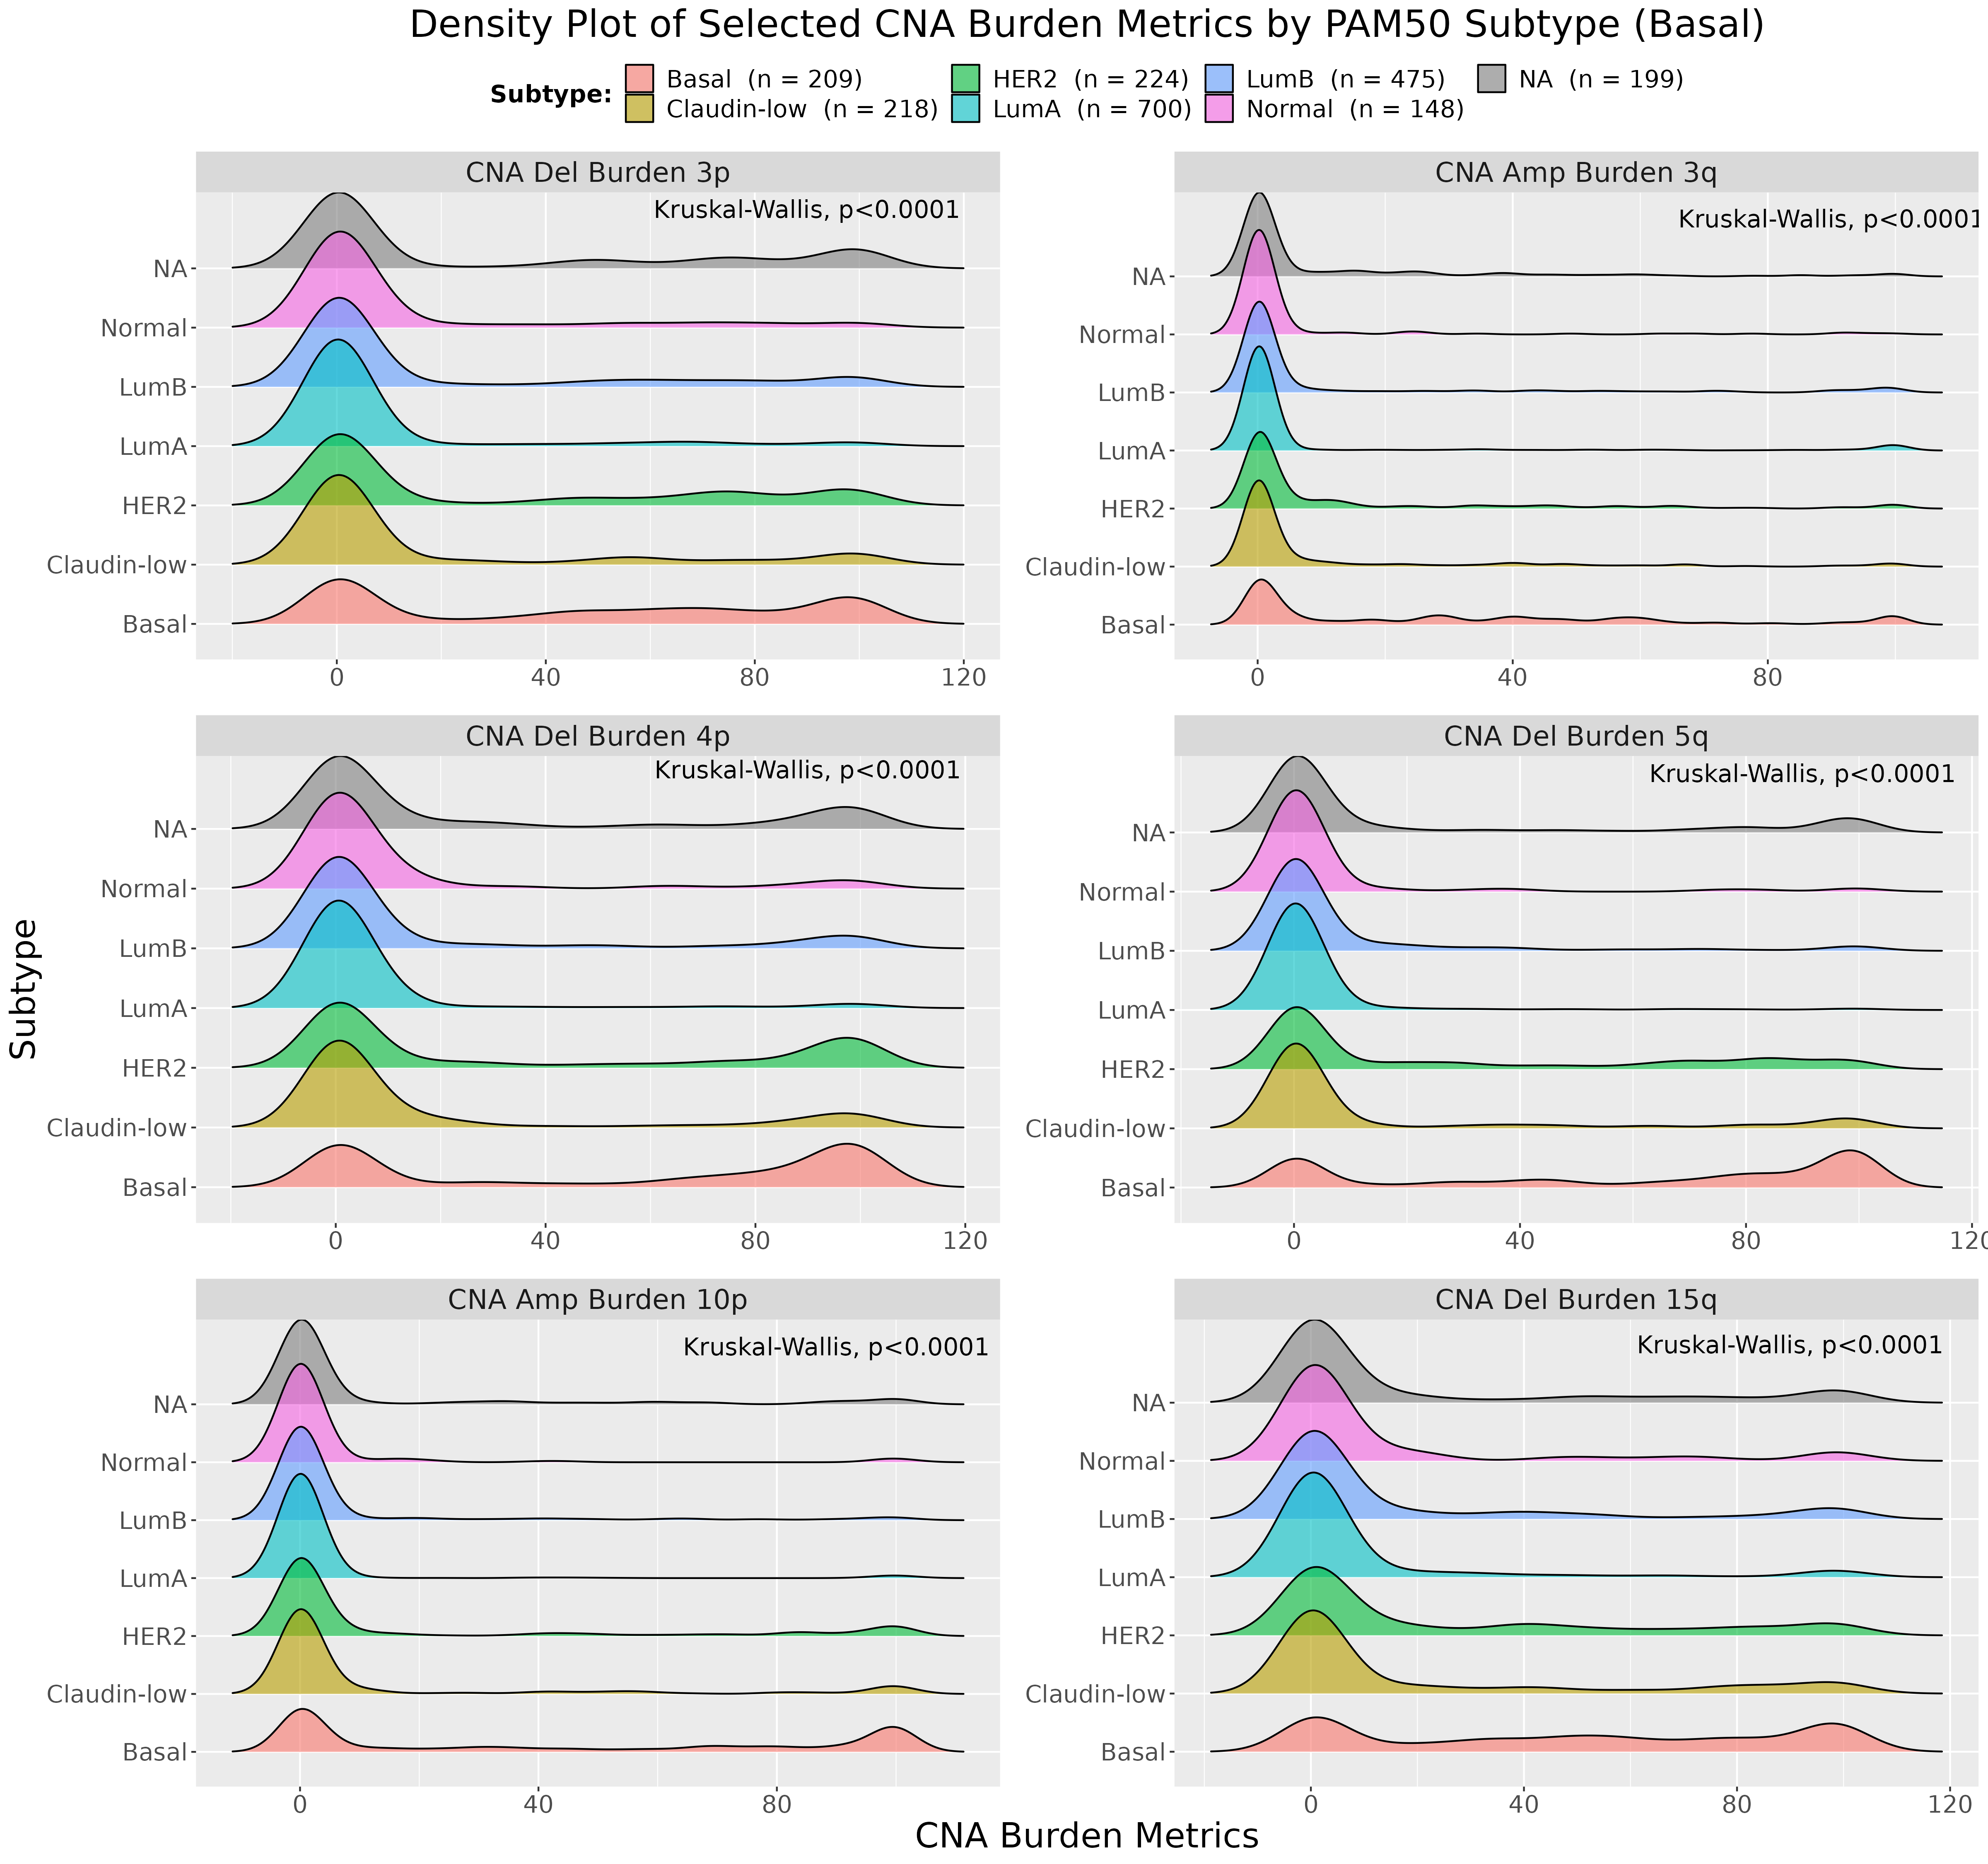
\includegraphics[width=1\textwidth]{../figures/Chapter_2/ChrArm_CNA_Burden_Metrics_Across_PAM50_Basal_Burden.png}
\caption[Density plots for each selected chromosome arm CNA Burden metrics, with a focus on the Basal subtype.]{Density plots for each selected chromosome arm CNA Burden metrics, with a focus on the Basal subtype. Chromosome arms where Basal patients display high GI are selected. Each facet contains boxplots for the chromosome arm CNA Burden metrics calculated using all available data and Benjamini-Hochberg adjusted Kruskal-Wallis p-values.}
\label{fig:PA-CNA-Score-Metric-Density-P50-5q}
\end{figure}
\vfill

\begin{table}[!htb]
\center
\caption[Comparisons of selected chromosome arm CNA Burden metric distributions by PAM50 subtype, with a focus on the Basal subtype.]{Comparisons of selected chromosome arm CNA Burden metric distributions by PAM50 subtype, with a focus on the Basal subtype. Chromosome arms where Basal patients display high GI are selected. Z statistics and Benjamini-Hochberg adjusted p-values are shown.}
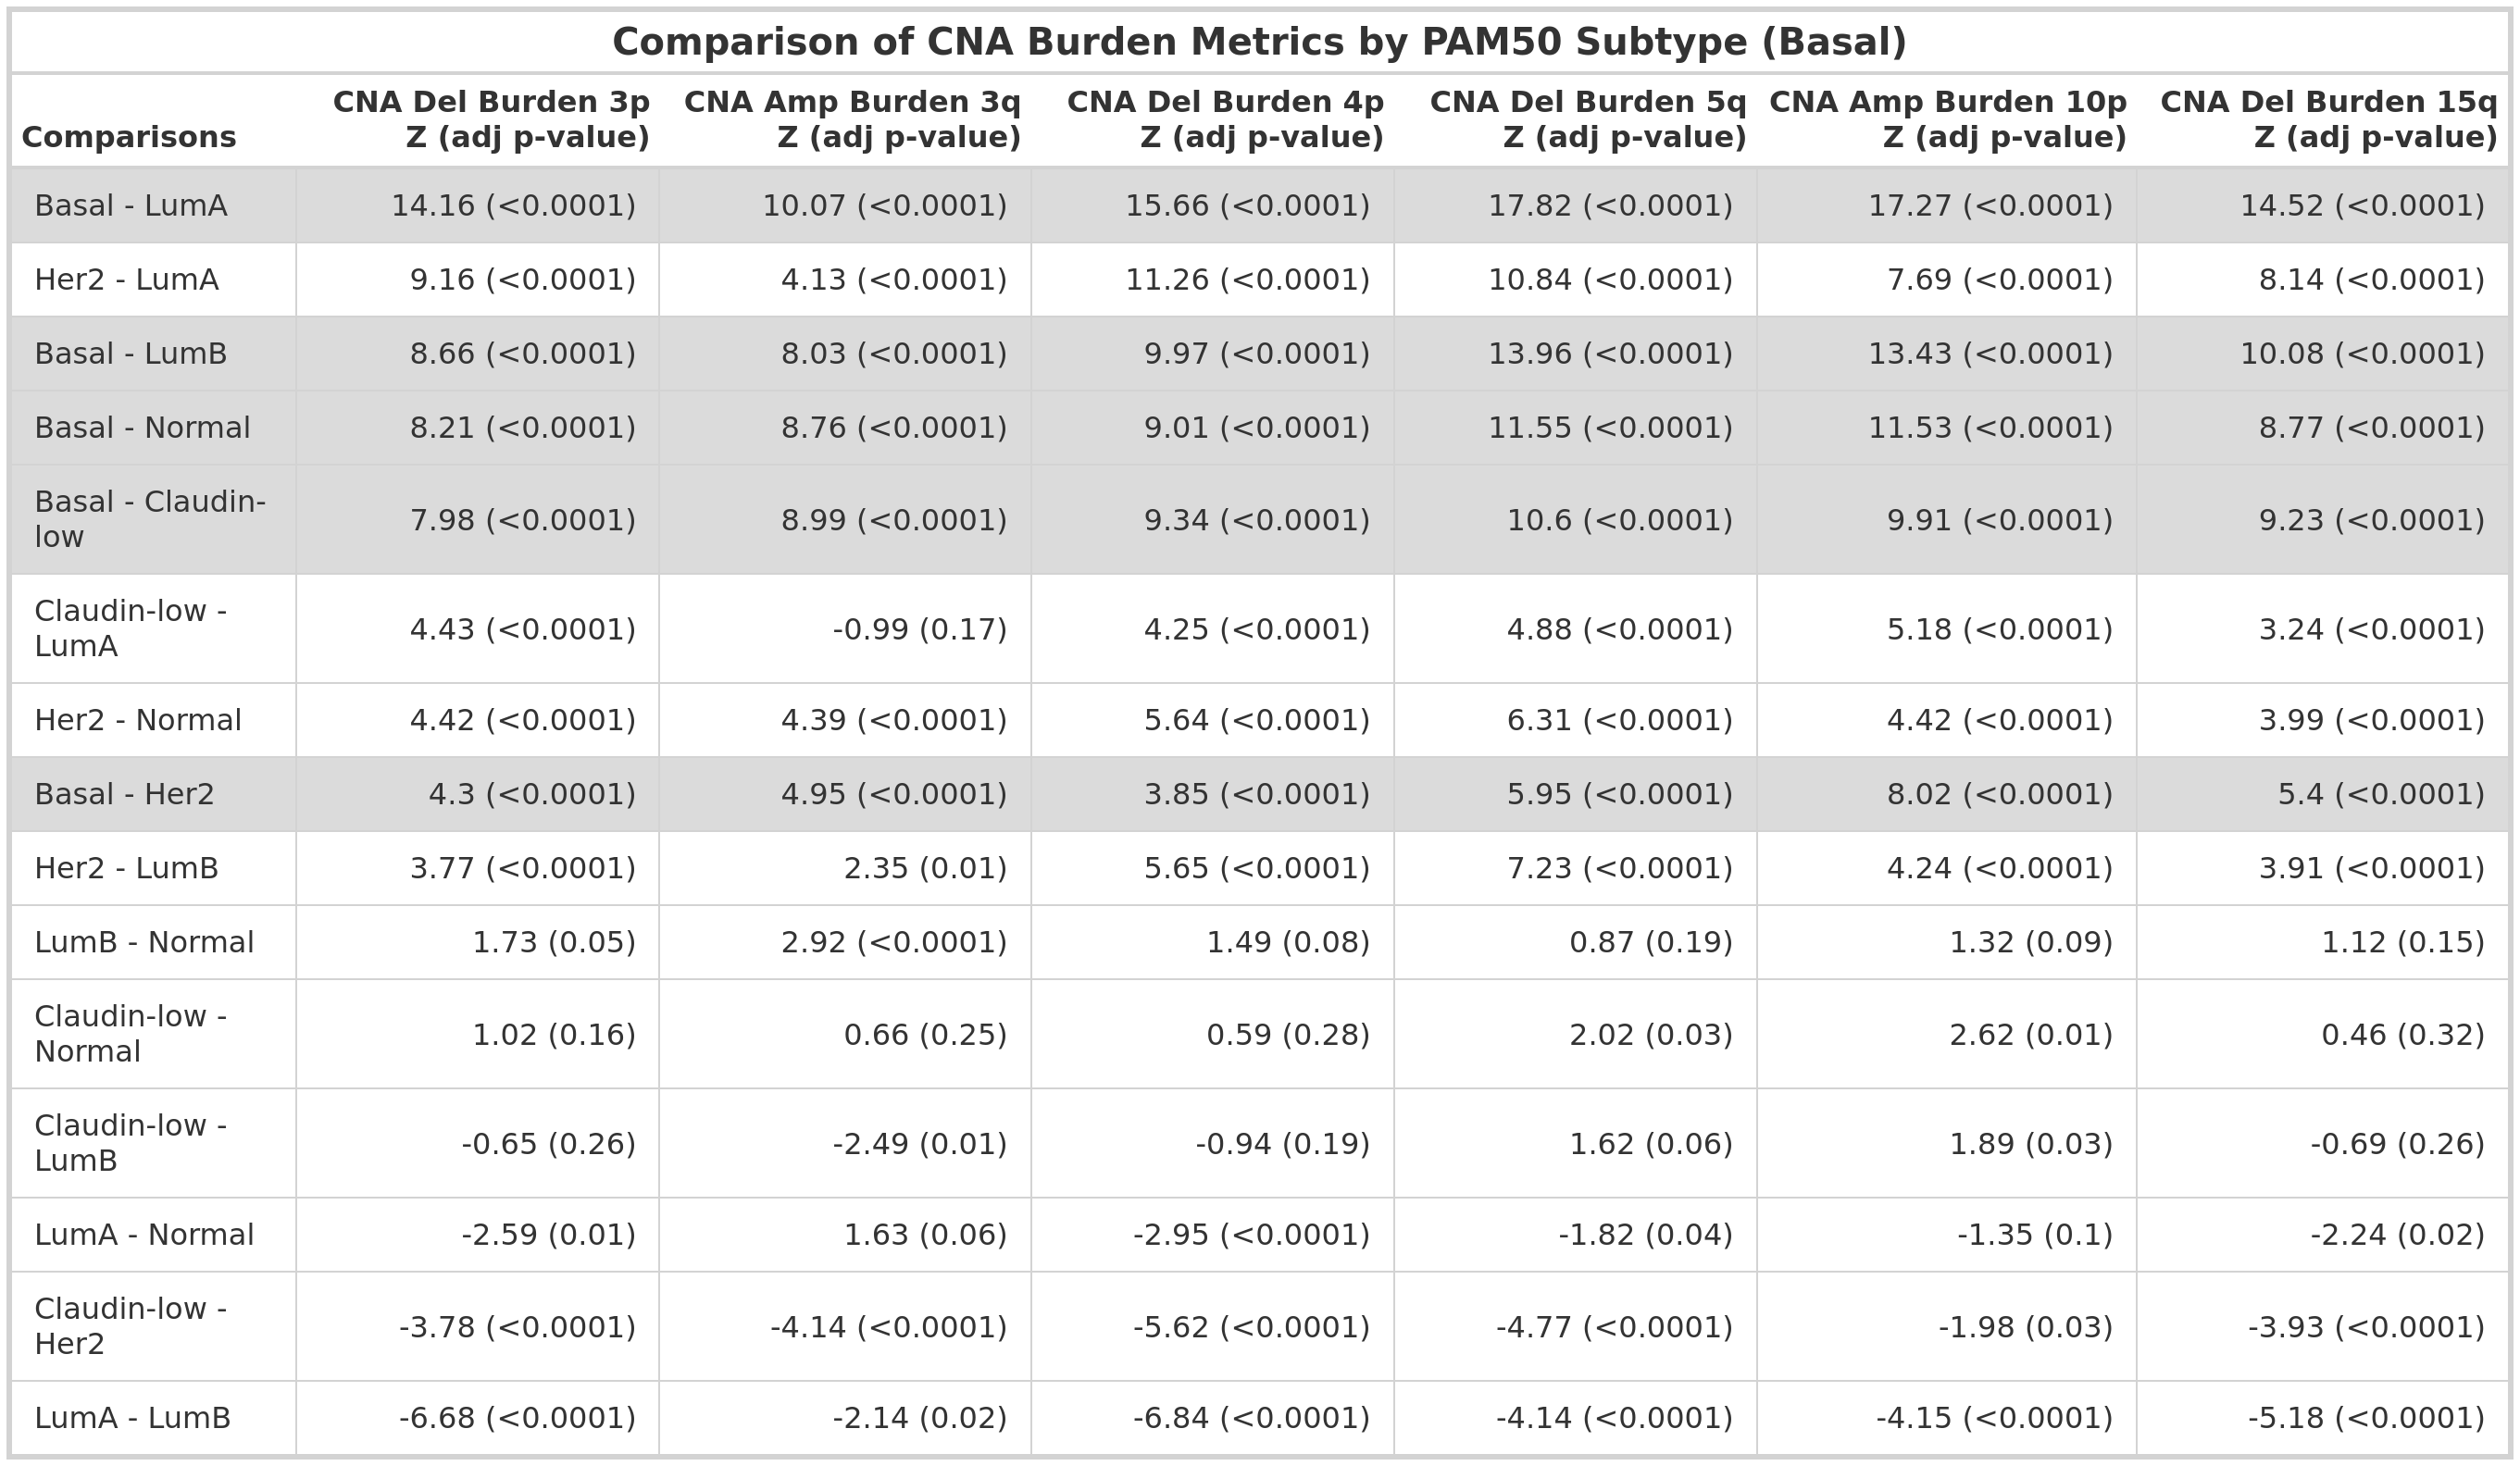
\includegraphics[width=1\textwidth]{../tables/Chapter_2/ChrArm_CNA_Burden_Metric_Comparisons_Basal.png}
\label{tab:PA-CNA-Score-Metric-Density-P50-5q}
\end{table}

\begin{figure}[!ht]
\center
\includegraphics[width=1\textwidth]{../figures/Chapter_2/ChrArm_CNA_Burden_Metrics_Across_PAM50_HER2_Burden.png}
\caption[Density plots for each selected chromosome arm CNA Burden metrics, with a focus on the HER2 subtype.]{Density plots for each selected chromosome arm CNA Burden metrics, with a focus on the HER2 subtype. Chromosome arms where HER2 patients display high GI are selected. Each facet contains boxplots for the chromosome arm CNA Burden metrics calculated using all available data and Benjamini-Hochberg adjusted Kruskal-Wallis p-values.}

\label{fig:PA-CNA-Score-Metric-Density-P50-17q}
\end{figure}

\begin{figure}[!htb]
\center
\includegraphics[width=1\textwidth]{../figures/Chapter_2/ChrArm_CNA_Burden_Metrics_Across_PAM50_Luminal_Burden.png}
\caption[Density plots for each selected chromosome arm CNA Burden metrics, with a focus on the Luminal subtype.]{Density plots for each selected chromosome arm CNA Burden metrics, with a focus on the Luminal subtype. Chromosome arms where Luminal patients display high GI are selected. Each facet contains boxplots for the chromosome arm CNA Burden metrics calculated using all available data and Benjamini-Hochberg adjusted Kruskal-Wallis p-values.}
\label{fig:PA-CNA-Score-Metric-Density-P50-16q}
\end{figure}

\begin{figure}[!htb]
\center
\includegraphics[width=1\textwidth]{../figures/Chapter_2/ChrArm_CNA_Burden_Metrics_Across_IC.png}
\caption[Density plots for each selected chromosome arm CNA Burden metrics across Integrative Cluster.]{Density plots for each selected chromosome arm CNA Burden metrics across Integrative Cluster. Each facet contains boxplots for the chromosome arm CNA Burden metrics calculated using all available data and Benjamini-Hochberg adjusted Kruskal-Wallis p-values.}
\label{fig:PA_IC}
\end{figure}

\begin{table}[!htb]
\center
\caption[Comparisons of selected chromosome arm CNA Burden metric distributions by PAM50 subtype, with a focus on the HER2 subtype.]{Comparisons of selected chromosome arm CNA Burden metric distributions by PAM50 subtype, with a focus on the HER2 subtype. Chromosome arms where HER2 patients display high GI are selected. Z statistics and Benjamini-Hochberg adjusted p-values are shown.}
\includegraphics[width=0.9\textwidth]{../tables/Chapter_2/ChrArm_CNA_Burden_Metric_Comparisons_HER2.png}
\label{tab:PA-CNA-Score-Metric-Density-P50-17q}
\end{table}

\begin{table}[!htb]
\center
\caption[Comparisons of selected chromosome arm CNA Burden metric distributions by PAM50 subtype, with a focus on the Luminal subtype.]{Comparisons of selected chromosome arm CNA Burden metric distributions by PAM50 subtype, with a focus on the Luminal subtype. Chromosome arms where Luminal patients display high GI are selected. Z statistics and Benjamini-Hochberg adjusted p-values are shown.}
\includegraphics[width=0.9\textwidth]{../tables/Chapter_2/ChrArm_CNA_Burden_Metric_Comparisons_Luminal.png}
\label{tab:PA-CNA-Score-Metric-Density-P50-16q}
\end{table}

\begin{table}[!htb]
\caption[Comparisons of selected chromosome arm CNA Burden metric distributions by Integrative Cluster.]{Comparisons of selected chromosome arm CNA Burden metric distributions by Integrative Cluster. Z statistics and Benjamini-Hochberg adjusted p-values are shown.}
\begin{minipage}[c]{0.45\textwidth}
\centering
\begin{tabular}{ccc}
\includegraphics[width=0.98\textwidth]{../tables/Chapter_2/ChrArm_CNA_Burden_Metric_Comparisons_IC_1.png}
\end{tabular}
\end{minipage}
\hspace{0.8cm}
\begin{minipage}[c]{0.45\textwidth}
\centering
\begin{tabular}{ccc}
\includegraphics[width=0.96\textwidth]{../tables/Chapter_2/ChrArm_CNA_Burden_Metric_Comparisons_IC_2.png}
\end{tabular}
\end{minipage}
\label{tab:PA_IC}
\end{table}
\clearpage 

\subsection{Conclusions}
GI plays an important role in the initiation and progression of cancer and can influence patient prognosis. There are myriad ways to try to quantify the levels of GI within tumour samples, from both gene expression and CNA data, a number of these and their limitations have been discussed in this chapter.

We proposed a number of novel CNA Score and Burden metrics quantifying GI of a patient, calculated globally across the full genome and for each chromosome arm. These comprehensible metrics, applicable to publicly available data, quantify GI in totality for all aberration types, and also quantify GI attributed to amplifications and deletions.

It was observed that the presence of missing values, in existence for some patients, has a negligible effect on both the global and chromosome arm CNA metric distributions. As a result, the approach of using all of the available patient CNA Score and Burden data, as opposed to including only complete cases, is adopted in the downstream analysis. Analysing distributions of the CNA metrics comparing groups of patients stratified by molecular classifications PAM50 and IntClust offered interesting observations. We see concordance with characteristic genomic aberrations documented previously, such as high quantification of deletion burden on chromosome 5q within Basal tumours and high quantification of amplification on chromosome 17q within HER2 tumours. Focusing on the direct comparison of levels of amplification metrics to deletion metrics, we observe the subtypes associated with worse OS and DSS tend to have significantly higher quantified deletion burden. As the deletion landscape of breast cancer has been poorly characterised, our novel findings that PAM50 and IntClust classifications with poorer OS and DSS have higher levels of GI, in particular higher CNA deletion burden, encourage further investigation.

In the next chapter we investigate how the quantified levels of CNA Scores and Burden correlate with survival outcomes. 

\section{Association of Copy Number Alteration Signatures and Survival Outcomes}
Time-to-event analysis is often used to estimate the extent to which potential biomarkers can differentiate on outcomes of disease progression, survival, recurrence, and response to treatment \citep{kleinbaum_klein_2012}. Time-to-event analysis focuses on the length of time until the occurrence of an event. This event may be the time to death from the disease, time to death from other causes, time to relapse or time to response to treatment. The data utilised in survival analysis are often termed survival data and have two key characteristics: that the response variable, representing the time to event occurrence, is a non-negative discrete or continuous random variable and that censoring is present. Censoring occurs when there is some information about an individual's time-to-event/survival time, but the time is not precisely observed. There are several reasons why an observation may be censored, such as the case where an individual has withdrawn from the study, where an individual is lost to follow-up during the study period, or where an individual has not experienced the event in the study period. These cases are all examples of right censoring. Other forms of censoring include left censoring, where the event of interest has already occurred before the study starts, and interval censoring, where the event occurs at an unknown time in an interval. Thus, survival data comprise a measurement indicating survival time and a binary indicator of the outcome occurring \citep{kleinbaum_klein_2012, moore_2016}. 

The primary goals of survival analysis are to estimate and interpret survival and/or hazard functions from sample survival data, to compare survival and/or hazard functions across stratified subcohorts of patients and to assess the relationship of candidate predictor variables in modelling time to event \citep{kleinbaum_klein_2012}. Statistical methods for modelling the survival and hazard functions can be categorised into parametric, semi-parametric and non-parametric techniques \citep{kleinbaum_klein_2012}. Parametric approaches are used when the survival time is assumed to follow an identifiable probability distribution such as the Weibull distribution \citep{pmid25220693}. The most common non-parametric approach in application is the Kaplan-Meier estimator \citep{kaplan58} of the survival function with log-rank tests \citep{pmid15117797} to compare survivor functions and the most commonly applied semi-parametric approach is the Cox proportional hazards (CPH) regression \citep{Cox}, used for modelling the association between survival time and one or more predictor variables. Survival trees, a more recent non-parametric approach, employ machine learning techniques to sequentially partition patients into groups that display similarity in survival functions \citep{pmid31896241}.  

This chapter presents an overview of survival analysis, discusses parametric, semi-parametric, and non-parametric survival approaches, with application to the METABRIC cohort, to measure any association of the derived and quantified CNA Score and Burden metrics on survival outcomes. This will assess the prognostic potential of the CNA metrics, alone and in combination with selected clinical and molecular features, and as such help identify patients who may be at a higher risk.

\subsection{Survival Analysis Methods}
Two critical functions in survival analysis are the survivor function ($S(t)$) and hazard function ($h(t)$) \citep{kleinbaum_klein_2012}. The survivor function is a function of time $t$ and denotes the probability that a person survives longer than some specified time $t$. Another way to think about the survivor function is the probability of a patient not experiencing an event. This function provides survival probabilities for different values of $t$, giving a full summary of the survival distribution, and can be specified by: 

\begin{equation}
S(t) = P(T > t) = 1-F(t) = \int_t^\infty f(u) du
\label{eq:EQ1}
\end{equation}

where $T$ represents a random variable denoting time to event occurring, e.g. the time from diagnosis to occurrence of death or disease relapse, and $F(t)$ is the cumulative distribution function for $T$. Theoretically, as $t$ goes from 0 to infinity, the survivor function can be graphed as a smooth curve, and has the following properties:   

\begin{itemize}
\item Is a non-increasing function.    

\item The probability of surviving past time 0 is 1, i.e. under the assumption the cohort under observation present at the beginning of the study without occurrence of the event, $S(t) = S(0) = 1$. 

\item As time goes to infinity the survivor curve tends towards 0, i.e. at time $t = \infty$,  $S(t) = S(\infty) = 0$. However, as observed in a cure model, it is possible for $S(\infty) > 0$.   
\end{itemize}

In contrast to the survivor function, the hazard function ($(h(t))$) gives the instantaneous rate of failure per unit time, given that the individual has survived up to time $t$ and is specified as: 

\begin{equation}
h(t) = \displaystyle{\lim_{\Delta t\to 0} \frac{P(t\leq T < t+\Delta t| T \geq t)}{\Delta t}} = \frac{f(t)}{S(t)}
\label{eq:EQ2}
\end{equation}

where $\Delta t$ denotes a small interval of time. For a particular value of $t$, $h(t)$ has the following characteristics: 

\begin{itemize}
\item $h(t)$ is always non-negative, i.e. $h(t) \geq 0$ for all $t >0$. 

\item $h(t)$ has no upper bound.
\end{itemize}

Like the survivor function, the hazard function can be graphed where $t$ is on the x-axis and $h(t)$ is on the y-axis. In this case, $h(t)$ does not have to start at 1, it may start anywhere and fluctuate up and down over time. These characteristics result in the hazard function taking on different forms depending on the nature of the study. For example, in a study where an individual remains healthy for the course of study, their instantaneous potential for event occurrence remains constant so that in this case, $h(t)$ remains the same constant value for all $t$. When the hazard function is constant, the survival model is called exponential. Another example might be a study of cancer patients and their response to treatment, where the event of interest is death due to disease. In this case the patient's potential for the event occurring, i.e. death, increases as $t$ increases. This is called an increasing Weibull model. Other types of hazard functions include the decreasing Weibull model ($h(t)$ decreases over time), the lognormal survival model ($h(t)$ increases and then decreases over time) and the bathtub model ($h(t)$ decreases and then increases over time).

Even though these two functions differ in the fact that $S(t)$ directly describes survival and $h(t)$ is a measure of instantaneous potential, if $S(t)$ or $h(t)$ is known, then the other may be determined. The relationship between $S(t)$ and $h(t)$ can be expressed using: 

\begin{equation}
S(t) = exp(-\int_0^th(u)du)
\label{eq:EQ3}
\end{equation}

\begin{equation}
h(t) = -(\frac{dS(t)/dt}{S(t)})
%\label{eq:EQ4}
\end{equation}

In parametric survival models the response, survival time, is assumed to follow an identifiable probability distribution. Parametric models are used in cases where information about the event process in a population point towards a particular distribution and once this probability density function, $f(t)$, is defined for survival time, the survivor and hazard functions can be calculated using Equations \ref{eq:EQ1} and \ref{eq:EQ2}. Some commonly used distributions include exponential, Weibull, log-logistic, generalised gamma, and lognormal. The main appeal in using parametric survival models include their simplicity and completeness. In the case where the assumed parametric model is correct, the parameter estimates can completely specify the survival and hazard functions. However, the use of parametric survival models is not always appropriate or sufficiently flexible and, in these cases, semi-parametric or non-parametric survival models may be used \citep{kleinbaum_klein_2012}.   

Semi-parametric models have both parametric and non-parametric components. An example of a semi-parametric survival model is the CPH model \citep{Cox, kleinbaum_klein_2012}. The CPH model uses non-parametric methods to estimate some baseline hazard, i.e. leaves the distribution of the baseline hazard function unspecified, and parametric methods to estimate the influence of predictor variables. The CPH model enables the incorporation of one or more predictor variables and as such is commonly used to investigate the association between survival and one or more categorical or continuous predictor variables, while accounting for possible confounders. Some examples of clinical predictor variables used in the context of breast cancer survival include number of lymph-nodes positive, tumour size, tumour grade, tumour subtype, ER/PR/HER2 status and type of treatment. 

Although this model is semi-parametric and as such does not require knowledge of the underlying distribution, it does have required assumptions. Two of the main assumptions are that hazard functions of different individuals are assumed to be proportional over time $t$ and the relationship between the log hazard and each predictor is assumed to be linear. Violations of these assumptions may lead to inaccurate results, i.e. biased effect estimates, and reduced statistical power \citep{pmid35070171}. These assumptions can be tested using the Schoenfeld and Martingale residuals \citep{Patil_Dessai_2019}. 

The CPH model facilitates quantification of the differences in survival distribution between groups. This is done by estimating the hazard ratio, defined as the ratio of the event rate at any given time in one group relative to another group. The CPH regression model can be written as follows: 

\begin{equation}
h(t, X) = h_0(t) \times exp(\sum_{i=1}^{p}\beta_iX_i)
\end{equation}

where $h(t)$ is the expected hazard at time $t$, $h_0(t)$ is the baseline hazard function that determines the shape of the survivor function and represents the hazard when all of the predictors are equal to zero, the $X_{i}$ represent the predictor variables in the model and the $\beta_i$ are the regression coefficients. The predicted hazard, i.e. $h(t)$, is the product of the baseline hazard $h_0(t)$ and the exponential function of the linear combination of the predictors, having a multiplicative or proportional effect on the predicted hazard. 

Since there is a corresponding relationship between $S(t)$ and $h(t)$, when a CPH model is applied survival estimates can be obtained that adjust for the explanatory variables used as predictors in the model. Using Equation \ref{eq:EQ3} the survivor function corresponding to the CPH regression model can be written as follows: 

\begin{equation}
S(t|X) = exp(-\int_0^th(u)du \times exp(\sum_{i=1}^{p}\beta_iX_i)) = S_0(t)^{exp(\beta'X)}
\end{equation}

where $S_0(t)$ is the baseline survivor function and $exp(\beta'X)$ is called the prognostic index. This survivor function is the basis for producing adjusted survival curves.

The CPH model is popular in application for many reasons. One of the main reasons is that even though the baseline hazard, $h_0(t)$, is an unspecified function, the CPH model is robust and therefore will closely approximate the results for the correct parametric model, i.e. provide good estimates of regression coefficients, hazard ratios of interest, and adjusted survival curves. Other properties of the CPH model that make it appealing include that the model will always produce non-negative hazard ratios, an estimated baseline hazard function is not necessary for the estimation of the hazard ratio and there are many widely available computer packages supporting application of CPH models. Of course, there are cases where the assumptions of the CPH model are not met and, in those cases, non-parametric methods may be considered \citep{kleinbaum_klein_2012}.

In cases where parametric and semi-parametric survival models are not appropriate or sufficiently flexible, non-parametric methods, not making any specific assumptions about the distribution of survival time, are applicable, we focus on two such approaches, the Kaplan-Meier (KM) estimator and survival trees.

\subsubsection{Kaplan-Meier Estimator}
In the case where there are no censored observations in the survival data, the survivor function can be estimated using the empirical survivor function, where, as the sample size increases the function will approach the shape of the population’s true survivor function. In this case the survivor function can be estimated using: 

\begin{equation}
\hat{S}(t) = \frac{\text{Number of observations with } T > t}{\text{Total sample size}}
\end{equation}

However, cases where there are no censored observations in the data are rare and so an extension of this method, termed the KM estimate, was developed to analyse survival data with censoring \citep{kaplan58}. The survivor function is estimated using the KM estimator and is defined as the fraction of observations that survived for a certain amount of time under the same circumstances, e.g. after treatment or disease diagnosis, and is given by the following formula: 

\begin{equation}
\hat{S}(t) = P(T > t) = \prod_{t_i \leq t} (1-\frac{d_i}{n_i})
\end{equation}

where $n_i$ is the number of subjects at risk at time $t_i$, and $d_i$ is the number of subjects who fail at time $t_i$.

The KM estimator is a continuous decreasing step function that starts at a survival probability of 1 and then steps down as you move from one ordered failure time to another, i.e.  each step down represents the occurrence of the event of interest for at least one observation. Censoring times only affect the estimate by reducing the size of the risk set for the next event, and thereby increasing the height of the next step down. To visualise this function, KM survival curves (plots of the KM estimator over time) are used. On a survival curve the y-axis represents the probability that the subject has not yet experienced the event of interest after surviving up to time $t$ and the x-axis represents time $t$. 

As an example, Figure \ref{fig:SurvivalCurves} provides the KM survival curves for DSS time, i.e. time from breast cancer diagnosis to the date of death from the disease, estimated from application to the HER- and HER2+ stratified patients observed in the METABRIC cohort. Figure \ref{fig:SurvivalCurves} illustrates the role of HER2 status as a biomarker: patients with HER2- breast cancer display more favourable DSS than patients with HER2+ breast cancer. The median survival time is 286 months for the HER2- group compared to 125 months for the HER2+ group. 

\vfill 
\begin{figure}[!h]
\includegraphics[width=1\textwidth]{../figures/Chapter_3/Example_Survival_Curve.png}
\caption[Kaplan-Meier plot for disease-specific survival in METABRIC patients stratified by HER2 status.]{Kaplan-Meier plot for disease-specific survival in METABRIC patients stratified by HER2 status. Lines corresponding to median disease-specific survival time for each group and the p-value associated with the log-rank test are displayed.}
\label{fig:SurvivalCurves}
\end{figure}
\vfill
\clearpage 

To determine whether two or more survival curves are significantly different from each other, a large-sample $\chi^2$ test (the log-rank test) tests the null hypothesis of no difference between the populations in the probability of an event at any time point. In Figure \ref{fig:SurvivalCurves}, the $p<0.0001$ indicates a significant difference in DSS comparing HER2- and HER2+ patients. 

\subsubsection{Recursive Partitioning Survival Trees}
Recursive partitioning techniques or tree-based methods were first developed by \cite{Morgan_Sonquist_1963} but were popularised in the 1980s following the development of the Classification and Regression Tree (CART) by Breiman et al. \citep{breiman_1984, bb_2011}. More recently, conditional inference trees (CTREE) have been developed to resolve some of the limitations of CART including overfitting and selection bias towards variables with many possible splits, i.e. continuous variables \citep{hothorn_hornik_zeileis_2006}. These non-parametric techniques are useful for identifying important predictors and structure in a dataset.  

These techniques recursively partition the data to form groups, called nodes, containing individuals with homogenous response values. The predicted response value for each node is then generally either the mean or mode dependent on whether the partitioning variable is continuous or categorical. Within the CART methodology, splits within the tree are arrived at by minimising a measure of node impurity. For categorical response variables measures of impurity may be the Gini index or information index. The Gini index denotes the probability that a random observation is misclassified when chosen randomly, while the information index relates to how much information is gained by splitting a set of data on a particular feature. For continuous response variables this measure may be the sum of squared deviations from the mean. The CTREE methodology differs in that the splits within the tree are arrived at using p-values from permutation-based significance tests.  

Using the CART or CTREE methodologies to produce predictive models has a number of advantages which are detailed below: 

\begin{enumerate}
\item No distributional assumptions are made. 
\item The predictor variables used can be continuous, interval or categorical. 
\item Robust to outliers, collinearities and heteroscedasticity. 
\item Can detect interactions and structure in a highly complex dataset. 
\item Transformations of the data do not change the structure of the tree. 
\item Can use the same variable multiple times, i.e. at different branches in the tree.
\end{enumerate}

To apply CART and CTREE methodologies available R packages include rpart \citep{therneau1997introduction} and partykit \citep{hothorn_hornik_zeileis_2006, ctree1}. 

The rpart procedure \citep{therneau1997introduction} implements many of the ideas found in CART and builds classification models (predicts a continuous value based on the predictor variables) or regression models (predicts discrete labels or categories based on the predictor variables) which can be represented as binary trees. The rpart algorithm is an iterative algorithm where the tree is built by first identifying a single variable which best splits the data into two groups. The same process is then applied separately to each sub-group, and so on recursively until the subgroups either reach a minimum size or until no improvement can be made. To split the data, rpart uses one of several measures of impurity such as the Gini index of a node and then chooses the split with maximal impurity reduction.

The CTREE procedure, applied in partykit \citep{hothorn_hornik_zeileis_2006, ctree1}, carries out variable selection and splitting in two steps, mitigating the tendency towards predictor variables with many possible splits or many missing values. Rather than employing information measures for predictor selection, CTREE applies a significance test procedure. The conditional distribution of statistics measuring the association between responses and predictor variables is responsible for the unbiased selection of variables that are measured on different scales. In addition, this algorithm applies multiple testing procedures to determine if there is no significant association between any of the predictors and the response and as such decides when the recursion should be halted. 

\subsection{CNA Metrics Stratify Luminal Breast Cancer Patients to Explain Survival Outcome}
Approximately 70\% of breast cancers are classified as Luminal A or B, characterised by increased levels of ER and PR \citep{pmid27341628}. Luminal B tumours tend to grow faster than Luminal A tumours, are of a higher grade, have a slightly worse prognosis and usually require more aggressive treatments. It has been suggested that the relationship between Luminal A and Luminal B tumours may be a continuum rather than a strict division of subtypes \citep{pmid18662380, pmid22522925, pmid27341628}. It has also been hypothesised that Luminal A tumours may evolve into Luminal B tumours as a result of stochastic acquisitions of mutations in genes associated with worse prognosis, including HER2 and tumour protein p53 (TP53) \citep{PfefferUlrich2013CGMc}. This ambiguity in Luminal classification may account for the variation that exists in DSS outcome for some Luminal A patients \citep{pmid27341628, pmid26679376, pmid30849944, pmid37253056}.

With focus and application to the Luminal METABRIC patients (n = 1,175, data downloaded from cBioPortal in 2019) we aim to explore whether the metrics of GI, specifically Absolute CNA Score, can add value in modelling OS and DSS within this group. 

\subsubsection{Preliminary Survival Analysis using Absolute CNA Score and Quartiles}
To explore estimated survival curves applying KM, the continuous Absolute CNA Score (Equation \ref{eq:CNA1}) was categorised into 4 levels: Q1, Q2, Q3, Q4. Each patient is recorded as one of these levels based on whether their Absolute CNA Score was in the first quartile (lowest GI) to fourth quartile (highest GI) relative to the observed Luminal METABRIC cohort (Figure \ref{fig:Lum_Dense}). 

KM fitted to patients stratified by the four levels of Absolute CNA Score Quartile indicate significant differences between the four estimated OS curves (log-rank test $p < 0.0001$, Figure \ref{fig:OS-Survival-Luminal}). The Absolute CNA Score Quartiles are associated with OS in Luminal breast cancer patients. Those in Absolute CNA Score Q4 (highest GI) have worse survival outcomes than patients with less GI in Absolute CNA Score Quartiles 1-3 (Q1-3). For DSS outcomes, KM fitted to patients stratified by the four levels of Absolute CNA Score Quartile indicates significant differences between the four estimated DSS curves (log-rank $p < 0.0001$, Figure \ref{fig:DSS-Survival-Luminal}). Luminal breast cancer patients in Q4 have worse DSS outcomes than patients in Q1-3. 

\begin{figure}[!h]
\centering
\includegraphics[width=0.98\textwidth]{../figures/Chapter_3/Luminal_AB_Score_Density.png}
\caption[Density plot of Absolute CNA Score distribution for METABRIC Luminal cases.]{Density plot of Absolute CNA Score distribution for METABRIC Luminal cases. Absolute CNA Score Quartiles 1-4 indicated by legend colours.}
\label{fig:Lum_Dense}
\end{figure}

\begin{figure}[!h]
\centering
\includegraphics[width=0.98\textwidth]{../figures/Chapter_3/Luminal_AB_Score_OS.png}
\caption[Kaplan-Meier plot for overall survival for METABRIC Luminal breast cancer patients in each Absolute CNA Score Quartile.]{Kaplan-Meier plot for overall survival for METABRIC Luminal breast cancer patients in each Absolute CNA Score Quartile. The p-value associated with the log-rank test and a risk table displaying the number of patients at risk at each time interval is displayed.}
\label{fig:OS-Survival-Luminal}
\end{figure}


\begin{figure}[!h]
\centering
\includegraphics[width=0.98\textwidth]{../figures/Chapter_3/Luminal_AB_Score_DSS.png}
\caption[Kaplan-Meier plot for disease-specific survival for METABRIC Luminal breast cancer patients in each Absolute CNA Score Quartile.]{Kaplan-Meier plot for disease-specific survival for METABRIC Luminal breast cancer patients in each Absolute CNA Score Quartile. The p-value associated with the log-rank test and a risk table displaying the number of patients at risk at each time interval is displayed.}
\label{fig:DSS-Survival-Luminal}
\end{figure}

To maintain the information from the uncategorised, quantitative measure of Absolute CNA Score, univariate Cox models were fitted for OS and DSS. The results obtained indicate that the Absolute CNA Score is associated with both OS (Hazard Ratio (HR) = 1.00 [1.00-1.00], $p < 0.001$) and DSS (HR = 1.00 [1.00-1.00], $p < 0.0001$).

\subsubsection{Analysis of Potential Confounding Variables and Multivariable Cox Models}
Having observed that Absolute CNA Score can independently help stratify Luminal patients into groups of similar survival outcome, it is important to assess whether Absolute CNA Score can add value in combination with other biomarkers. KM plots and univariate Cox models were used to determine if any of the 23 available clinical variables (list in Appendix A) were associated with survival outcome. It was found that 19 of the clinical variables considered were associated with OS and 18 were associated with DSS (Tables \ref{tab:Surv_Tests_OS} and \ref{tab:Surv_Tests_DSS}). The clinical variables found to be significant within the univariate analysis were examined for possible associations with the Absolute CNA Scores and Absolute CNA Score Quartiles, applying tests such as the $\chi^2$ test, Fisher’s exact test, Kruskal-Wallis test and Pearson's correlation, as appropriate to the variable type. These tests indicated that the Absolute CNA Scores and CNA Score Quartiles were significantly associated with a number of clinical variables (Tables \ref{tab:Assoc_Tests_S} and \ref{tab:Assoc_Tests_Q}).

Since highly correlated predictors may lead to unreliable and unstable estimates of regression coefficients \citep{Keith_2019}, a refined selection of variables were considered based on understanding of the clinical definition of the variable, e.g. HER2 Status and HER2 SNP6 use different methods to capture similar information (discussed further in \cite{King_2021}). Eight candidate clinical predictors remained: PAM50 subtype, histological grade, tumour size, number of lymph nodes positive, age, HER2 status, PR status and histological subtype. These eight candidate clinical predictors were considered along with either the Absolute CNA Score or Absolute CNA Score Quartile variable in multivariable CPH models for OSS and DSS. Under the assumption of proportional hazards, the results indicated that the Absolute CNA Score metric was significantly associated with the outcome in a model for DSS along with six clinical predictors: PAM50 subtype, histological grade, tumour size, number of positive lymph nodes, age at diagnosis, and HER2 status, both using the categorical CNA Score Quartiles (Table \ref{table_mcm}) and the original continuous Absolute CNA Scores (Table \ref{table_mcms}). 

\vfill
\begin{table}[!h]
\caption[Overall survival univariate Cox models for each clinical variable.]{Overall survival univariate Cox models for each clinical variable. Likelihood ratio test (LRT) and Wald test p-values and Benjamini-Hochberg adjusted p-values are displayed.}
\includegraphics[width=0.98\textwidth]{../tables/Chapter_3/Luminal_Survival_Association_OS.png}
\label{tab:Surv_Tests_OS}
\end{table}
\vfill
\clearpage
\begin{table}[!ht]
\caption[Disease-specific survival univariate Cox models for each clinical variable.]{Disease-specific survival univariate Cox models for each clinical variable. Likelihood ratio test (LRT) and Wald test p-values and Benjamini-Hochberg adjusted p-values are displayed.}
\includegraphics[width=0.98\textwidth]{../tables/Chapter_3/Luminal_Survival_Association_DSS.png}
\label{tab:Surv_Tests_DSS}
\end{table}

As the focus and application here is only within Luminal cancers, PAM50 subtype has only two levels Luminal A and Luminal B. In the fitted models an indicator variable assumes the reference group to be Luminal A, and the estimated effect using this indicator is for Luminal B relative to Luminal A. In the model using Absolute CNA Scores the reference group is Luminal A, histological grade 1, HER2-negative patients (Table \ref{table_mcms}). For Luminal A patients, Absolute CNA Score is associated with DSS (HR = 1.00 [1.00-1.00], $p < 0.001$). For Luminal B patients, the effect of Absolute CNA Score on DSS is estimated by fitting interaction effects between Absolute CNA Score and PAM50 subtype. This indicates that the association between Absolute CNA Score is significantly different for Luminal B patients compared to Luminal A patients (HR = 1.00 [0.99-1.00], $p < 0.012$). Setting Luminal B as the reference group indicates that for Luminal B patients, Absolute CNA Score is not associated with DSS.  

In the model using Absolute CNA Score Quartiles the reference group is Luminal A, histological grade 1, HER2-negative patients with Absolute CNA Scores with lowest GI level, Absolute CNA Score Q1 (Table \ref{table_mcm}). Comparing Absolute CNA Score Q4 to CNA Q1, within Luminal A patients, shows a significant increased risk in DSS (HR = 2.32 [1.36-3.94], $p = 0.002$). Comparing Absolute CNA Score Q3 to Absolute CNA Score Q1, within Luminal A patients, shows a significant increased risk in DSS (HR = 2.15 [1.33-3.49], $p = 0.002$). There was no evidence of a significant effect on risk comparing Absolute CNA Score Q2 Luminal A patients to Absolute CNA Score Q1 Luminal A patients (HR = 1.37 [0.83 - 2.27], $p = 0.219$). For Luminal B patients, the effect of Absolute CNA Score Quartile on DSS differs in comparison to Luminal A patients estimated by fitting interaction effects between Absolute CNA Score Quartiles and PAM50 subtype, the effect is a reduction in the estimated difference comparing Absolute CNA Score Quartile within Luminal B. 


\begin{table}[!htb]
\caption[Association tests between Absolute CNA Score and selected clinical variables.]{Association tests between Absolute CNA Score and selected clinical variables. Kruskal-Wallis and Pearson's Correlation p-values and Benjamini-Hochberg adjusted p-values are displayed.}
\includegraphics[width=0.98\textwidth]{../tables/Chapter_3/CNA_Score_Clin_Association.png}
\label{tab:Assoc_Tests_S}
\end{table}

\begin{table}[!htb]
\caption[Association tests between Absolute CNA Score Quartiles and selected clinical variables.]{Association tests between Absolute CNA Score Quartiles and selected clinical variables. $\chi^2$, Fisher's Exact and Kruskal-Wallis test p-values and Benjamini-Hochberg adjusted p-values are displayed.}
\includegraphics[width=0.98\textwidth]{../tables/Chapter_3/CNA_Quartile_Clin_Association.png}
\label{tab:Assoc_Tests_Q}
\end{table}

Plotting the adjusted survival curves for Luminal A and Luminal B patients within the different Absolute CNA Score Quartiles illustrates how these estimated effects differ between the two subtypes. Adjusted survival curves represent the estimated effect of Absolute CNA Score Quartiles by plotting the predicted survival curves for Luminal A and Luminal B patients for each Absolute CNA Score Quartile, having adjusted for the effects of the other covariates in the multivariable Cox model, where other covariates are fixed at the median/mode values of those variables (Figure \ref{fig:CNAQuartileSurvivalAdusted}). Here we see that DSS curves comparing Absolute CNA Score Quartiles within Luminal A show significant differences while the differences observed in DSS curves comparing Absolute CNA Score Quartiles within Luminal B are small and non-significant.  

\begin{table}[!htb]
\tiny
\caption[Final multivariable CPH model for disease-specific survival (Absolute CNA Score Quartiles).]{Final multivariable CPH model for disease-specific survival. Including selected clinical variables, Absolute CNA Score Quartiles and an interaction term, within the Luminal METABRIC cohort.}
\centering
\resizebox{\textwidth}{!}{ 
    \begin{tabular}{lccccl}
    \hline
    \textbf{Clinical Variable} & \textbf{Beta} & \textbf{SE} & \textbf{HR} & \textbf{95\% CI} & \textbf{P-value} \\ 
    \hline
    PAM50: &  &  &  &  & \\ 
    Luminal A (Ref) & - & - & - & - & - \\ 
    Luminal B & 1.069 & 0.299 & 2.912 & (1.619 - 5.237) & $<$0.001 \\
    Histological Grade: &  &  &  &  & \\
    1 (Ref) & - & - & - & - & -\\ 
    2 & 0.381 & 0.254 & 1.464 & (0.889 - 2.410) & 0.134 \\ 
    3 & 0.528 & 0.262 & 1.696 & (1.014 - 2.837) & 0.044 \\ 
    Tumour Size & 0.015 & 0.003 & 1.015 & (1.010 - 1.020) & $<$0.001 \\
    Positive Lymph Nodes & 0.050 & 0.008 & 1.051 & (1.034 - 1.069) & $<$0.001 \\ 
    Age at Diagnosis & 0.018 & 0.005 & 1.018 & (1.008 - 1.029) & $<$0.001 \\ 
    HER2 Status: &  &  &  &  & \\ 
    Negative (Ref) & - & - & - & - & - \\ 
    Positive & 0.541 & 0.202 & 1.717 & (1.157 - 2.550) & 0.007\\ 
    CNA Quartile: &  &  &  &  & \\ 
    CNA Q1 (Ref) & - & - & - & - & - \\ 
    CNA Q2 & 0.315 & 0.256 & 1.370 & (0.829 - 2.265) & 0.219 \\ 
    CNA Q3 & 0.767 & 0.247 & 2.152 & (1.326 - 3.493) & 0.002\\ 
    CNA Q4 & 0.839 & 0.272 & 2.315 & (1.360 - 3.942) & 0.002 \\ 
    CNA Q2:LumB  & -0.764 & 0.395 & 0.466 & (0.215 - 1.010) & 0.053  \\
    CNA Q3:LumB & -0.730 & 0.364 & 0.482 & (0.236 - 0.983) & 0.045 \\ 
    CNA Q4:LumB & -0.909 & 0.370 & 0.403 & (0.195 - 0.831) & 0.014 \\ \hline
    Likelihood Ratio Test p-value & & & & & \textless{2e-16} \\
    Wald Test p-value & & & & & \textless{2e-16}\\
    Score (log-rank) Test p-value  & & & & &\textless{2e-16} \\  \hline 
    \multicolumn{7}{l}{\begin{tabular}[c]{@{}l@{}} 
        SE: Standard Error; HR: Hazard Ratio; CI: Confidence Interval
        \label{table_mcm}
        \end{tabular}} \\ \hline
    \end{tabular}}
\end{table}

\begin{table}[!htb]
\tiny
\caption[Final multivariable CPH model for disease-specific survival (Absolute CNA Score).]{Final multivariable CPH model for disease-specific survival. Including selected clinical variables, Absolute CNA Score and an interaction term, within the Luminal METABRIC cohort.}
\centering
\resizebox{\textwidth}{!}{ 
    \begin{tabular}{lccccl}
    \hline
    \textbf{Clinical Variable} & \textbf{Beta} & \textbf{SE} & \textbf{HR} & \textbf{95\% CI} & \textbf{P-value} \\ 
    \hline
    PAM50: &  &  &  &  & \\ 
    Luminal A (Ref) & - & - & - & - & - \\ 
    Luminal B & 0.896 & 0.225 & 2.450 & (1.576 - 3.808) & $<$0.001 \\
    Histological Grade: &  &  &  &  & \\
    1 (Ref) & - & - & - & - & - \\ 
    2 & 0.431 & 0.253 & 1.539 & (0.937 - 2.525) & 0.088 \\ 
    3 & 0.636 & 0.260  & 1.888  & (1.135 - 3.141) & 0.014 \\ 
    Tumour Size & 0.013 & 0.002 & 1.013 & (1.009 - 1.018) & $<$0.001 \\
    Positive Lymph Nodes & 0.049 &  0.009 & 1.050 & (1.033 - 1.068) & $<$0.001 \\ 
    Age at Diagnosis & 0.016 & 0.005 & 1.016 & (1.006 - 1.027) & 0.002 \\ 
    HER2 Status: &  &  &  &  & \\ 
    Negative (Ref) & - & - & - & - & - \\ 
    Positive & 0.568 & 0.201 & 1.765 & (1.191 - 2.615) & 0.005\\ 
    CNA Score & 6.05e-05 & 1.83e-05 & 1.000  & (1.000 - 1.000) & $<$0.001  \\ 
    CNA Score:LumB & -6.77e-05 & 2.69e-05 & 0.999 & (0.999 - 1.000) & 0.012\\ \hline
    Likelihood Ratio Test p-value & & & & & \textless{2e-16}\\
    Wald Test p-value & & & & & \textless{2e-16}\\
    Score (log-rank) Test p-value  & & & & &\textless{2e-16}\\  \hline 
    \multicolumn{7}{l}{\begin{tabular}[c]{@{}l@{}}
        SE: Standard Error; HR: Hazard Ratio; CI: Confidence Interval
        \label{table_mcms}
        \end{tabular}} \\ \hline
    \vspace{0.2cm}
    \end{tabular}}
\end{table}

\begin{figure}[!htb]
\centering
\begin{subfigure}[b]{0.49\linewidth}       
\centering
\includegraphics[width=\linewidth]{../figures/Chapter_3/LuminalA_Adsurvplot.png}
\caption{Luminal A Patients}
\label{fig:A}
\end{subfigure}
\begin{subfigure}[b]{0.49\linewidth}        
\centering
\includegraphics[width=\linewidth]{../figures/Chapter_3/LuminalB_Adsurvplot.png}
\caption{Luminal B Patients}
\label{fig:B}
\end{subfigure}
\caption[Adjusted survival curves for estimated Absolute CNA Score Quartile effects within each Luminal PAM50 subtype.]{Adjusted survival curves for estimated Absolute CNA Score Quartile effects within each Luminal PAM50 subtype. (A) Luminal A and (B) Luminal B breast cancer patients.}
\label{fig:CNAQuartileSurvivalAdusted}
\end{figure}
\FloatBarrier 

\subsubsection{Implementation of Recursive Partitioning Survival Trees}
Although the fitted models give strong indication that Absolute CNA Score, both as a continuous and categorical metric, can add value in modelling survival outcome in Luminal breast cancer, diagnostic tests indicate that the proportional hazards assumption may not be met (online Supplementary Information). As an alternative approach, recursive partitioning survival trees are fitted using the rpart and ctree algorithms. Recursive partitioning trees can explore the association between Absolute CNA Score and survival and examine any interactions between the six clinical variables that were significant in models including Absolute CNA Score variables. The predetermined Absolute CNA Score Quartiles can be fitted in the model as a predictor, but recursive partitioning trees also offer the added benefit of determining the optimum cut-off in Absolute CNA Score, implicit in the partitioning algorithm. 

Survival trees considering Absolute CNA Score Quartiles, with additional applications provided in Appendix A, suggest a similar partitioning with Absolute CNA Score Q1 and Q2 versus Absolute CNA Score Q3 and Q4, consistent with the effects estimated by the CPH model (Figure \ref{fig:LumAB_Trees_Quart}). Figure \ref{fig:LumAB_Trees_Quart} shows the survival tree fitted using the ctree algorithm, which indicates that for Luminal A patients who have 0-1 positive lymph nodes, tumour size less than 31mm and age of diagnosis less than 71.4 years, DSS outcome can be stratified by Absolute CNA Score Quartile, where patients with high GI show reduced survival probability than those with a lower GI ($p = 0.032$).   

Survival trees considering Absolute CNA Score, with additional applications provided in Appendix A, also suggest a similar partitioning consistent with the effects estimated by the CPH model and the survival trees considering Absolute CNA Score Quartiles (Figure \ref{fig:LumAB_Trees_Score}). In Figure \ref{fig:LumAB_Trees_Score}, the survival tree fitted using the ctree algorithm, Luminal A patients who have 0-1 positive lymph nodes, tumour size less than 31mm and age of diagnosis less than 71.4 years, DSS outcome can be stratified by Absolute CNA Score with optimised Absolute CNA Score cut-off point value 5,882 ($p = 0.005$). Including the continuous Absolute CNA Score, rather than the categorised Absolute CNA Score Quartile, allows a more nuanced investigation of the optimal Absolute CNA Score cut-off point. While the estimated optimal cut-off of 5,882 is close to 5,547, the boundary between Absolute CNA Score Quartile 2 and 3, utilising the Absolute CNA Score cut-off results in 20 patients being reclassified to the low-risk group.  

Overall, the survival trees indicate that the Absolute CNA Score metric, implemented either as predetermined categorised quartiles or original continuous variable, can stratify subsets of patients based on DSS and therefore help identify Luminal A patients who are at elevated risk.  

\begin{figure}[!htb]
\centering
\includegraphics[width=\linewidth]{../figures/Chapter_3/LuminalAB_Ctree_DSS_Quart.png}
\caption[Recursive partitioning survival tree for disease-specific survival using clinical variables and Absolute CNA Score Quartile as candidate predictors (ctree).]{Recursive partitioning survival tree for disease-specific survival using clinical variables and Absolute CNA Score Quartile as candidate predictors. Fitted using the ctree algorithm.}
\label{fig:LumAB_Trees_Quart}
\end{figure}

\begin{figure}[!htb]
\centering
\includegraphics[width=\linewidth]{../figures/Chapter_3/LuminalAB_Ctree_DSS_Score.png}
\caption[Recursive partitioning survival tree for disease-specific survival using clinical variables and Absolute CNA Score as candidate predictors (ctree).]{Recursive partitioning survival tree for disease-specific survival using clinical variables and Absolute CNA Score as candidate predictors. Fitted using the ctree algorithm.}
\label{fig:LumAB_Trees_Score}
\end{figure}
\clearpage

\subsection{Analysis of Global CNA Metrics across All METABRIC Patients}
Expanding the study focus to all patients, i.e. all PAM50 subtypes (Basal, HER2, Luminal B, Luminal A, Normal and Claudin-low), associations between the six global CNA Score metrics and six global CNA Burden metrics with survival are examined in this section. The global CNA metrics are initially included with PAM50 subtype or IntClust molecular classifications to assess whether the CNA metric information can add additional prognostic value to the molecular classifications, and then included with a selection of clinical variables to explore interactions between the clinical variables and CNA metrics. Given the large number of candidate predictors under consideration, the fact that the CPH assumption may not be met, and the benefit of the partitioning trees in determining optimal cut-off, recursive partitioning survival trees are implemented. 

\subsubsection{CNA Metric Survival Trees in Combination with Molecular Classification Predictors} 
A range of survival trees for OS, DSS, 5-year OS and DSS, and 10-year OS and DSS are produced. These trees include the six global CNA Score metrics: Absolute CNA Score, CNA Amp Score, CNA Del Score, Difference Score, Percentage Amp Score and Percentage Del Score, or the six global CNA Burden metrics: CNA Burden, CNA Amp Burden, CNA Del Burden, Difference Burden, Percentage Amp Burden and Percentage Del Burden, with PAM50 subtype or IntClust molecular classifications. Depending on the algorithm used (rpart or ctree) a number of different global CNA Score and Burden metrics are selected as useful predictors when modelling survival outcomes. The survival trees for DSS outcomes are displayed and discussed below, while the survival trees for OS outcomes are provided in Appendix B. 

Initially survival trees including only PAM50 subtype (Figure \ref{fig:PAM50_Indv_Surv_Trees}) or IntClust (Figure \ref{fig:IC_Indv_Surv_Trees}) as candidate predictors are fitted, indicating which subtypes display similarity in survival outcome and providing information on partitions in trees where only molecular classification is included.

\captionsetup[subfigure]{font={normalfont, small}, skip=1pt, margin=-0.0cm, singlelinecheck=false}

\begin{figure}[!h]
\begin{minipage}{.44\textwidth}
\begin{subfigure}{\textwidth}
\subcaption{}
\includegraphics[width=\linewidth, height = 5.7cm]{../figures/Chapter_3/Ind_Partykit_Survival_Score_DSS_PAM50.png}
\end{subfigure}\par
\end{minipage}
\begin{minipage}{.55\textwidth}
\begin{subfigure}{\textwidth}
\subcaption{}
\includegraphics[width=\linewidth, height = 5.7cm]{../figures/Chapter_3/Ind_Ctree_Survival_Score_DSS_PAM50.png}
\end{subfigure}\par
\end{minipage}

\caption[Recursive partitioning survival trees for disease-specific survival using PAM50 subtype as a candidate predictor.]{Recursive partitioning survival trees for disease-specific survival using PAM50 subtype as a candidate predictor. (A) Trees fitted using the rpart algorithm and (B) trees fitted using the ctree algorithm.}
\label{fig:PAM50_Indv_Surv_Trees}
\end{figure}

\begin{figure}[!h]
\begin{minipage}{.44\textwidth}
\begin{subfigure}{\textwidth}
\subcaption{}
\includegraphics[width=\linewidth, height = 5.7cm]{../figures/Chapter_3/Ind_Partykit_Survival_Score_DSS_INTCLUST.png}
\end{subfigure}\par
\end{minipage}
\begin{minipage}{.55\textwidth}
\begin{subfigure}{\textwidth}
\subcaption{}
\includegraphics[width=\linewidth, height = 5.7cm]{../figures/Chapter_3/Ind_Ctree_Survival_Score_DSS_INTCLUST.png}
\end{subfigure}\par
\end{minipage}

\caption[Recursive partitioning survival trees for disease-specific survival using Integrative Cluster as a candidate predictor.]{Recursive partitioning survival trees for disease-specific survival using Integrative Cluster as a candidate predictor. (A) Trees fitted using the rpart algorithm and (B) trees fitted using the ctree algorithm.}
\label{fig:IC_Indv_Surv_Trees}
\end{figure}

Focusing on survival trees for DSS, 5-year DSS and 10-year DSS, that have the six CNA Score metrics and PAM50 molecular classification as candidate predictors, indicates CNA Del Score to be a consistently significant factor (Figure \ref{fig:PAM50_CNA_Score_DSS}, \ref{fig:PAM50_CNA_Score_FiveYearDSS} and \ref{fig:PAM50_CNA_Score_TenYearDSS}). While variation in the predictors used to partition the data is observed across survival outcome (DSS, 5-year DSS or 10-year DSS) and algorithm (rpart or ctree), CNA Del Score appears to add additional prognostic value to the PAM50 subtypes, primarily Luminal A and Claudin-low subtypes. Patients within these subtypes, displaying higher levels of CNA Del Score, have poorer outcome with respect to DSS, 5-year and 10-year DSS. Consistency is observed in the CNA Del Score cut-off points chosen by the ctree algorithm across the three survival outcomes. The optimal cut-off point for CNA Del Score for trees produced using the ctree algorithm is 3,286 in Luminal A and Claudin-low patients (Figure \ref{fig:PAM50_CNA_Score_DSS}B), 3,286 in Luminal A patients (Figure \ref{fig:PAM50_CNA_Score_FiveYearDSS}B), and 3,138 in Luminal A, Claudin-low and Normal patients (Figure \ref{fig:PAM50_CNA_Score_TenYearDSS}B), for DSS, 5-year DSS and 10-year DSS. 

When considering the survival trees for DSS, 5-year DSS and 10-year DSS, generated using the six CNA Burden metrics and PAM50 molecular classification as candidate predictors, similar tree structures are observed (Figures \ref{fig:PAM50_CNA_Burden_DSS}, \ref{fig:PAM50_CNA_Burden_FiveYearDSS}, and \ref{fig:PAM50_CNA_Burden_TenYearDSS}). CNA Del Burden is again consistently selected as an important predictor in the context of DSS, partitioning Luminal A and Claudin-low subtypes using a cut-off of 18.28\% (Figure \ref{fig:PAM50_CNA_Burden_DSS}B), 5-year DSS, partitioning Luminal A subtype using a cutoff of 14.55\% (Figure \ref{fig:PAM50_CNA_Burden_FiveYearDSS}B), and 10-year DSS, partitioning Luminal A, Claudin-low and Normal subtypes using a cutoff of 14.02\% (Figure \ref{fig:PAM50_CNA_Burden_TenYearDSS}B). 

In the survival trees for DSS, 5-year DSS and 10-year DSS, generated using the six CNA Score metrics and IntClust molecular classification as candidate predictors, CNA Del Score consistently appears as an important predictor for survival outcome, in patients corresponding to IntClust 3, 4ER+, 7 and 8 (Figures \ref{fig:INTCLUST_CNA_Score_DSS}-\ref{fig:INTCLUST_CNA_Score_TenYearDSS}). Again, the optimal cut-off points are fairly consistent, in all but one tree, at values 1,469.5 and 1,469 for DSS (Figure \ref{fig:INTCLUST_CNA_Score_DSS}), 1,933 and 3,722 for 5-year DSS (Figure \ref{fig:INTCLUST_CNA_Score_FiveYearDSS}), and 1,469.5 and 1,989 for 10-year DSS (Figure \ref{fig:INTCLUST_CNA_Score_TenYearDSS}). Patients within IntClust 3, 4ER+, 7 and 8, displaying levels of CNA Del Score above the optimal cut-off point have worse DSS, 5 and 10-year DSS, than patients displaying levels of CNA Del Score below the optimal cut-off point. 

Considering survival trees for DSS, 5-year DSS and 10-year DSS, with the six CNA Burden metrics and IntClust molecular classification as candidate predictors, indicate similar tree structures (Figures \ref{fig:INTCLUST_CNA_Burden_DSS}-\ref{fig:INTCLUST_CNA_Burden_TenYearDSS}). Again, all trees initially split on IntClust, with CNA Del Burden consistently selected as an additional significant predictor in the context of the DSS, 5-year DSS and 10-year DSS. 

It appears that the CNA Del Score and Burden metrics are associated with DSS, 5-year DSS and 10-year DSS. The majority of the survival trees showed that the CNA Del metrics are useful in splitting Luminal A and Claudin-low patients, and IntClust 3, 4ER+, 7 and 8 patients, into groups with distinct survival outcomes. Interestingly, a known feature of these PAM50 subtypes and IntClusts is that they display low genomic instability and good prognosis \citep{pmid22522925}, Section \ref{LGI}. This may explain why the optimal cut-off points for the CNA Del Score and Burden are quite low. In Chapter 2, we observed that PAM50 subtypes associated with poorer survival (Basal, HER2 and Luminal B) have significantly higher levels of deletions. Here, we observe that within PAM50/IntClust classifications associated with good prognosis, that have CNA Del Score and Burden over an optimised threshold, patients having poorer survival outcomes, again indicating that high levels of deletions are more detrimental than other forms of alterations.

\begin{figure}[!h]
\centering

\vspace{0.5cm}

\begin{subfigure}{\textwidth}
\subcaption{}
\includegraphics[width=1\textwidth]{../figures/Chapter_3/PartyKit_Survival_Score_DSS_PAM50.png}
\end{subfigure}

\vspace{2cm}

\begin{subfigure}{\textwidth}
\subcaption{}
\includegraphics[width=1\textwidth]{../figures/Chapter_3/Ctree_Survival_Score_DSS_PAM50.png}
\end{subfigure}

\vspace{0.5cm}

\caption[Recursive partitioning survival trees for disease-specific survival using PAM50 subtype and the six CNA Score metrics as candidate predictors.]{Recursive partitioning survival trees for disease-specific survival using PAM50 subtype and the six CNA Score metrics as candidate predictors. (A) Trees fitted using the rpart algorithm and (B) trees fitted using the ctree algorithm.}
\label{fig:PAM50_CNA_Score_DSS}
\end{figure}

\begin{figure}[!h]
\centering

\vspace{0.5cm}

\begin{subfigure}{\textwidth}
\subcaption{}
\includegraphics[width=1\textwidth]{../figures/Chapter_3/PartyKit_Survival_Score_FiveYearDSS_PAM50.png}
\end{subfigure}

\vspace{2cm}

\begin{subfigure}{\textwidth}
\subcaption{}
\includegraphics[width=1\textwidth]{../figures/Chapter_3/Ctree_Survival_Score_FiveYearDSS_PAM50.png}
\end{subfigure}

\vspace{0.5cm}

\caption[Recursive partitioning survival trees for five-year disease-specific survival using PAM50 subtype and the six CNA Score metrics as candidate predictors.]{Recursive partitioning survival trees for five-year disease-specific survival using PAM50 subtype and the six CNA Score metrics as candidate predictors. (A) Trees fitted using the rpart algorithm and (B) trees fitted using the ctree algorithm.}
\label{fig:PAM50_CNA_Score_FiveYearDSS}
\end{figure}

\begin{figure}[!h]
\centering

\vspace{0.5cm}

\begin{subfigure}{\textwidth}
\subcaption{}
\includegraphics[width=1\textwidth]{../figures/Chapter_3/PartyKit_Survival_Score_TenYearDSS_PAM50.png}
\end{subfigure}

\vspace{2cm}

\begin{subfigure}{\textwidth}
\subcaption{}
\includegraphics[width=1\textwidth]{../figures/Chapter_3/Ctree_Survival_Score_TenYearDSS_PAM50.png}
\end{subfigure}

\vspace{0.5cm}

\caption[Recursive partitioning survival trees for ten-year disease-specific survival using PAM50 subtype and the six CNA Score metrics as candidate predictors.]{Recursive partitioning survival trees for ten-year disease-specific survival using PAM50 subtype and the six CNA Score metrics as candidate predictors. (A) Trees fitted using the rpart algorithm and (B) trees fitted using the ctree algorithm.}
\label{fig:PAM50_CNA_Score_TenYearDSS}
\end{figure}


\begin{figure}[!h]
\centering

\vspace{0.5cm}

\begin{subfigure}{\textwidth}
\subcaption{}
\includegraphics[width=1\textwidth]{../figures/Chapter_3/PartyKit_Survival_Burden_DSS_PAM50.png}
\end{subfigure}
\vspace{2cm}

\begin{subfigure}{\textwidth}
\subcaption{}
\includegraphics[width=1\textwidth]{../figures/Chapter_3/Ctree_Survival_Burden_DSS_PAM50.png}
\end{subfigure}
\vspace{0.5cm}

\caption[Recursive partitioning survival trees for disease-specific survival using PAM50 subtype and the six CNA Burden metrics as candidate predictors.]{Recursive partitioning survival trees for disease-specific survival using PAM50 subtype and the six CNA Burden metrics as candidate predictors. (A) Trees fitted using the rpart algorithm and (B) trees fitted using the ctree algorithm.}
\label{fig:PAM50_CNA_Burden_DSS}
\end{figure}

\begin{figure}[!h]
\centering

\vspace{0.5cm}

\begin{subfigure}{\textwidth}
\subcaption{}
\includegraphics[width=1\textwidth]{../figures/Chapter_3/PartyKit_Survival_Burden_FiveYearDSS_PAM50.png}
\end{subfigure}
\vspace{2cm}


\begin{subfigure}{\textwidth}
\subcaption{}
\includegraphics[width=1\textwidth]{../figures/Chapter_3/Ctree_Survival_Burden_FiveYearDSS_PAM50.png}
\end{subfigure}
\vspace{0.5cm}

\caption[Recursive partitioning survival trees for five-year disease-specific survival using PAM50 subtype and the six CNA Burden metrics as candidate predictors.]{Recursive partitioning survival trees for five-year disease-specific survival using PAM50 subtype and the six CNA Burden metrics as candidate predictors. (A) Trees fitted using the rpart algorithm and (B) trees fitted using the ctree algorithm.}
\label{fig:PAM50_CNA_Burden_FiveYearDSS}
\end{figure}

\begin{figure}[!h]
\centering

\vspace{0.5cm}

\begin{subfigure}{\textwidth}
\subcaption{}
\includegraphics[width=1\textwidth]{../figures/Chapter_3/PartyKit_Survival_Burden_TenYearDSS_PAM50.png}
\end{subfigure}
\vspace{2cm}

\begin{subfigure}{\textwidth}
\subcaption{}
\includegraphics[width=1\textwidth]{../figures/Chapter_3/Ctree_Survival_Burden_TenYearDSS_PAM50.png}
\end{subfigure}
\vspace{0.5cm}

\caption[Recursive partitioning survival trees for ten-year disease-specific survival using PAM50 subtype and the six CNA Burden metrics as candidate predictors.]{Recursive partitioning survival trees for ten-year disease-specific survival using PAM50 subtype and the six CNA Burden metrics as candidate predictors. (A) Trees fitted using the rpart algorithm and (B) trees fitted using the ctree algorithm.}
\label{fig:PAM50_CNA_Burden_TenYearDSS}
\end{figure} 

\begin{figure}[!h]
\centering

\vspace{0.5cm}

\begin{subfigure}{\textwidth}
\subcaption{}
\includegraphics[width=1\textwidth]{../figures/Chapter_3/PartyKit_Survival_Score_DSS_INTCLUST.png}
\end{subfigure}

\vspace{2cm}

\begin{subfigure}{\textwidth}
\subcaption{}
\includegraphics[width=1\textwidth]{../figures/Chapter_3/Ctree_Survival_Score_DSS_INTCLUST.png}
\end{subfigure}

\vspace{0.5cm}

\caption[Recursive partitioning survival trees for disease-specific survival using Integrative Cluster and the six CNA Score metrics as candidate predictors.]{Recursive partitioning survival trees for disease-specific survival using Integrative Cluster and the six CNA Score metrics as candidate predictors. (A) Trees fitted using the rpart algorithm and (B) trees fitted using the ctree algorithm.}
\label{fig:INTCLUST_CNA_Score_DSS}
\end{figure}

\begin{figure}[!h]
\centering

\vspace{0.5cm}

\begin{subfigure}{\textwidth}
\subcaption{}
\includegraphics[width=1\textwidth]{../figures/Chapter_3/PartyKit_Survival_Score_FiveYearDSS_INTCLUST.png}
\end{subfigure}

\vspace{2cm}

\begin{subfigure}{\textwidth}
\subcaption{}
\includegraphics[width=1\textwidth]{../figures/Chapter_3/Ctree_Survival_Score_FiveYearDSS_INTCLUST.png}
\end{subfigure}

\vspace{0.5cm}

\caption[Recursive partitioning survival trees for five-year disease-specific survival using Integrative Cluster and the six CNA Score metrics as candidate predictors.]{Recursive partitioning survival trees for five-year disease-specific survival using Integrative Cluster and the six CNA Score metrics as candidate predictors. (A) Trees fitted using the rpart algorithm and (B) trees fitted using the ctree algorithm.}
\label{fig:INTCLUST_CNA_Score_FiveYearDSS}
\end{figure}

\begin{figure}[!h]
\centering

\vspace{0.5cm}

\begin{subfigure}{\textwidth}
\subcaption{}
\includegraphics[width=1\textwidth]{../figures/Chapter_3/PartyKit_Survival_Score_TenYearDSS_INTCLUST.png}
\end{subfigure}

\vspace{2cm}

\begin{subfigure}{\textwidth}
\subcaption{}
\includegraphics[width=1\textwidth]{../figures/Chapter_3/Ctree_Survival_Score_TenYearDSS_INTCLUST.png}
\end{subfigure}

\vspace{0.5cm}

\caption[Recursive partitioning survival trees for ten-year disease-specific survival using Integrative Cluster and the six CNA Score metrics as candidate predictors.]{Recursive partitioning survival trees for ten-year disease-specific survival using Integrative Cluster and the six CNA Score metrics as candidate predictors. (A) Trees fitted using the rpart algorithm and (B) trees fitted using the ctree algorithm.}
\label{fig:INTCLUST_CNA_Score_TenYearDSS}
\end{figure}

\begin{figure}[!h]
\centering

\vspace{0.5cm}

\begin{subfigure}{\textwidth}
\subcaption{}
\includegraphics[width=1\textwidth]{../figures/Chapter_3/PartyKit_Survival_Burden_DSS_INTCLUST.png}
\end{subfigure}

\vspace{2cm}

\begin{subfigure}{\textwidth}
\subcaption{}
\includegraphics[width=1\textwidth]{../figures/Chapter_3/Ctree_Survival_Burden_DSS_INTCLUST.png}
\end{subfigure}

\vspace{0.5cm}

\caption[Recursive partitioning survival trees for disease-specific survival using Integrative Cluster and the six CNA Burden metrics as candidate predictors.]{Recursive partitioning survival trees for disease-specific survival using Integrative Cluster and the six CNA Burden metrics as candidate predictors. (A) Trees fitted using the rpart algorithm and (B) trees fitted using the ctree algorithm.}
\label{fig:INTCLUST_CNA_Burden_DSS}
\end{figure}

\begin{figure}[!h]
\centering

\vspace{0.5cm}

\begin{subfigure}{\textwidth}
\subcaption{}
\includegraphics[width=1\textwidth]{../figures/Chapter_3/PartyKit_Survival_Burden_FiveYearDSS_INTCLUST.png}
\end{subfigure}

\vspace{2cm}

\begin{subfigure}{\textwidth}
\subcaption{}
\includegraphics[width=1\textwidth]{../figures/Chapter_3/Ctree_Survival_Burden_FiveYearDSS_INTCLUST.png}
\end{subfigure}

\vspace{0.5cm}

\caption[Recursive partitioning survival trees for five-year disease-specific survival using Integrative Cluster and the six CNA Burden metrics as candidate predictors.]{Recursive partitioning survival trees for five-year disease-specific survival using Integrative Cluster and the six CNA Burden metrics as candidate predictors. (A) Trees fitted using the rpart algorithm and (B) trees fitted using the ctree algorithm.}
\label{fig:INTCLUST_CNA_Burden_FiveYearDSS}
\end{figure}

\begin{figure}[!h]
\centering

\vspace{0.5cm}

\begin{subfigure}{\textwidth}
\subcaption{}
\includegraphics[width=1\textwidth]{../figures/Chapter_3/PartyKit_Survival_Burden_TenYearDSS_INTCLUST.png}
\end{subfigure}

\vspace{2cm}

\begin{subfigure}{\textwidth}
\subcaption{}
\includegraphics[width=1\textwidth]{../figures/Chapter_3/Ctree_Survival_Burden_TenYearDSS_INTCLUST.png}
\end{subfigure}

\vspace{0.5cm}

\caption[Recursive partitioning survival trees for ten-year disease-specific survival using Integrative Cluster and the six CNA Burden metrics as candidate predictors.]{Recursive partitioning survival trees for ten-year disease-specific survival using Integrative Cluster and the six CNA Burden metrics as candidate predictors. (A) Trees fitted using the rpart algorithm and (B) trees fitted using the ctree algorithm.}
\label{fig:INTCLUST_CNA_Burden_TenYearDSS}
\end{figure}


\begin{figure}[!h]
\centering

\vspace{1cm}

\begin{subfigure}{\textwidth}
\subcaption{}
\includegraphics[width=1\textwidth]{../figures/Chapter_3/Clin_PartyKit_Survival_Burden_DSS_PAM50.png}
\end{subfigure}

\vspace{3cm}

\begin{subfigure}{\textwidth}
\subcaption{}
\includegraphics[width=1\textwidth]{../figures/Chapter_3/Clin_Ctree_Survival_Burden_DSS_PAM50.png}
\end{subfigure}

\vspace{1cm}

\caption[Recursive partitioning survival trees for disease-specific survival using PAM50 subtype, the six CNA Burden metrics and a number of clinical variables as candidate predictors.]{Recursive partitioning survival trees for disease-specific survival using PAM50 subtype, the six CNA Burden metrics and a number of clinical variables as candidate predictors. (A) Trees fitted using the rpart algorithm and (B) trees fitted using the ctree algorithm.}
\label{fig:PAM50_CNA_Burden_DSS_Clin}
\end{figure}

\begin{figure}[!h]
\centering

\vspace{1cm}

\begin{subfigure}{\textwidth}
\subcaption{}
\includegraphics[width=1\textwidth]{../figures/Chapter_3/Clin_PartyKit_Survival_Burden_FiveYearDSS_PAM50.png}
\end{subfigure}

\vspace{3cm}

\begin{subfigure}{\textwidth}
\subcaption{}
\includegraphics[width=1\textwidth]{../figures/Chapter_3/Clin_Ctree_Survival_Burden_FiveYearDSS_PAM50.png}
\end{subfigure}

\vspace{1cm}

\caption[Recursive partitioning survival trees for five-year disease-specific survival using PAM50 subtype, the six CNA Burden metrics and a number of clinical variables as candidate predictors.]{Recursive partitioning survival trees for five-year disease-specific survival using PAM50 subtype, the six CNA Burden metrics and a number of clinical variables as candidate predictors. (A) Trees fitted using the rpart algorithm and (B) trees fitted using the ctree algorithm.}
\label{fig:PAM50_CNA_Burden_FiveYearDSS_Clin}
\end{figure}

\begin{figure}[!h]
\centering

\vspace{1cm}

\begin{subfigure}{\textwidth}
\subcaption{}
\includegraphics[width=1\textwidth]{../figures/Chapter_3/Clin_PartyKit_Survival_Burden_TenYearDSS_PAM50.png}
\end{subfigure}

\vspace{3cm}

\begin{subfigure}{\textwidth}
\subcaption{}
\includegraphics[width=1\textwidth]{../figures/Chapter_3/Clin_Ctree_Survival_Burden_TenYearDSS_PAM50.png}
\end{subfigure}

\vspace{1cm}

\caption[Recursive partitioning survival trees for ten-year disease-specific survival using PAM50 subtype, the six CNA Burden metrics and a number of clinical variables as candidate predictors.]{Recursive partitioning survival trees for ten-year disease-specific survival using PAM50 subtype, the six CNA Burden metrics and a number of clinical variables as candidate predictors. (A) Trees fitted using the rpart algorithm and (B) trees fitted using the ctree algorithm.}
\label{fig:PAM50_CNA_Burden_TenYearDSS_Clin}
\end{figure}

\begin{figure}[!h]
\centering

\vspace{1cm}

\begin{subfigure}{\textwidth}
\subcaption{}
\includegraphics[width=1\textwidth]{../figures/Chapter_3/Clin_PartyKit_Survival_Burden_DSS_INTCLUST.png}
\end{subfigure}

\vspace{3cm}

\begin{subfigure}{\textwidth}
\subcaption{}
\includegraphics[width=1\textwidth]{../figures/Chapter_3/Clin_Ctree_Survival_Burden_DSS_INTCLUST.png}
\end{subfigure}

\vspace{1cm}

\caption[Recursive partitioning survival trees for disease-specific survival using Integrative Cluster, the six CNA Burden metrics and a number of clinical variables as candidate predictors.]{Recursive partitioning survival trees for disease-specific survival using Integrative Cluster, the six CNA Burden metrics and a number of clinical variables as candidate predictors. (A) Trees fitted using the rpart algorithm and (B) trees fitted using the ctree algorithm.}
\label{fig:INTCLUST_CNA_Burden_DSS_Clin}
\end{figure}

\begin{figure}[!h]
\centering

\vspace{1cm}

\begin{subfigure}{\textwidth}
\subcaption{}
\includegraphics[width=1\textwidth]{../figures/Chapter_3/Clin_PartyKit_Survival_Burden_FiveYearDSS_INTCLUST.png}
\end{subfigure}

\vspace{3cm}

\begin{subfigure}{\textwidth}
\subcaption{}
\includegraphics[width=1\textwidth]{../figures/Chapter_3/Clin_Ctree_Survival_Burden_FiveYearDSS_INTCLUST.png}
\end{subfigure}

\vspace{1cm}

\caption[Recursive partitioning survival trees for five-year disease-specific survival using Integrative Cluster, the six CNA Burden metrics and a number of clinical variables as candidate predictors.]{Recursive partitioning survival trees for five-year disease-specific survival using Integrative Cluster, the six CNA Burden metrics and a number of clinical variables as candidate predictors. (A) Trees fitted using the rpart algorithm and (B) trees fitted using the ctree algorithm.}
\label{fig:INTCLUST_CNA_Burden_FiveYearDSS_Clin}
\end{figure}

\begin{figure}[!h]
\centering

\vspace{1cm}

\begin{subfigure}{\textwidth}
\subcaption{}
\includegraphics[width=1\textwidth]{../figures/Chapter_3/Clin_PartyKit_Survival_Burden_TenYearDSS_INTCLUST.png}
\end{subfigure}

\vspace{3cm}

\begin{subfigure}{\textwidth}
\subcaption{}
\includegraphics[width=1\textwidth]{../figures/Chapter_3/Clin_Ctree_Survival_Burden_TenYearDSS_INTCLUST.png}
\end{subfigure}

\vspace{1cm}

\caption[Recursive partitioning survival trees for ten-year disease-specific survival using Integrative Cluster, the six CNA Burden metrics and a number of clinical variables as candidate predictors.]{Recursive partitioning survival trees for ten-year disease-specific survival using Integrative Cluster, the six CNA Burden metrics and a number of clinical variables as candidate predictors. (A) Trees fitted using the rpart algorithm and (B) trees fitted using the ctree algorithm.}
\label{fig:INTCLUST_CNA_Burden_TenYearDSS_Clin}
\end{figure}

\subsubsection{CNA Metric Survival Trees in Combination with Molecular Classification and Clinical Predictors}
To assess how the addition of clinical variables alters the observed partitioning and explore interactions between the clinical variables and CNA metrics in modelling DSS, 5-year DSS and 10-year DSS, survival trees including the six CNA Burden metrics, IntClust or PAM50 molecular classification, and selected clinical variables as candidate predictors are fitted (Figures \ref{fig:PAM50_CNA_Burden_DSS_Clin}-\ref{fig:INTCLUST_CNA_Burden_TenYearDSS_Clin}). To avoid overcrowding, these trees are limited to a depth of four, where depth is defined as the number of layers or levels in the tree. While the CNA Score and CNA Burden trees partition the data similarly, it is observed that there is more consensus among the CNA Burden trees produced across different survival times and using different algorithms. Based on this and the fact that CNA Burden is a standardised metric, i.e. all patients have CNA Burden in the range 0 to 100, we show only the survival trees including CNA Burden, IntClust or PAM50 molecular classification, and selected clinical variables, as candidate predictors. The clinical variables selected are number of positive lymph nodes, NPI, ER Status, PR Status, HER2 Status, age, tumour size, tumour stage, tumour grade and cancer type.  

Figures \ref{fig:PAM50_CNA_Burden_DSS_Clin}-\ref{fig:PAM50_CNA_Burden_TenYearDSS_Clin} display survival trees for DSS, 5-year DSS and 10-year DSS, that have the six CNA Burden metrics, PAM50 molecular classification and the selected clinical variables as candidate predictors. It is observed that total CNA Burden, CNA Del Burden and Percentage Amp Burden, appear as significant predictors in the context of the DSS, in addition to PAM50 subtype and a number of clinical variables including NPI, number of positive lymph nodes, age and ER status.

For DSS, CNA Burden provides additional information for patients who have NPI $< 5.05$, and for patients who have NPI $< 5.05$ and $\leq 1$ positive lymph node, for the rpart and ctree algorithms, respectively (Figure \ref{fig:PAM50_CNA_Burden_DSS_Clin}). The CNA Burden threshold for both partitions are 24.91\% and 24.90\%. For the 5-year DSS survival trees, fitted with the rpart algorithm, CNA Burden with threshold 24.56\% is used \FloatBarrier \noindent to partition the patients with NPI $< 4.05$ and CNA Del Burden is used to partition patients with NPI $\geq 4.05$ and ER positivity, with threshold 10.85\% (Figure \ref{fig:PAM50_CNA_Burden_FiveYearDSS_Clin}A). For the 5-year DSS survival trees, fitted with the ctree algorithm, CNA Del Burden, with threshold 16.52\%, is used to split patients with NPI $\leq 5.05$ who correspond to the Claudin-low, Luminal A, Luminal B and Normal PAM50 subtypes (Figure \ref{fig:PAM50_CNA_Burden_FiveYearDSS_Clin}B). Similar partitions are observed in the 10-year DSS trees (Figure \ref{fig:PAM50_CNA_Burden_TenYearDSS_Clin}), where CNA Burden and CNA Del Burden are utilised in sub-partitions of the trees. Interestingly, even with the addition of traditionally used clinical variables, the CNA Burden metrics still appear useful in stratifying patients based on DSS, 5-year and 10-year DSS. In particular, CNA Del Burden is again used to partition Luminal A, Claudin-low and Normal patients. In all cases, patients in the partition corresponding to the lower GI have better disease-specific survival outcomes.

Focusing on survival trees for DSS, 5-year DSS and 10-year DSS, that have the six CNA Burden metrics, IntClust molecular classification and the selected clinical variables as candidate predictors, similar tree structures are observed. Again, CNA Burden, CNA Del Burden and Percentage Amp Burden appear to be useful in stratifying patients in the context of disease-specific survival (Figures \ref{fig:INTCLUST_CNA_Burden_DSS_Clin}-\ref{fig:INTCLUST_CNA_Burden_TenYearDSS_Clin}). 

\subsection{Analysis of Chromosome Arm CNA Metrics across All METABRIC Patients}
\label{Trees_Arm}
In addition to expanding the study focus to all patients, we also broaden the analysis by using the 42 chromosome arm CNA Score and Burden metrics as candidate predictors in the survival trees. These chromosome arm CNA metrics are initially included with PAM50 or IntClust molecular classifications to assess whether the chromosome arm CNA metric information can add additional prognostic value to the molecular classifications, and then included with a selection of clinical variables to explore interactions between the clinical variables and CNA metrics.

\subsubsection{Chromosome Arm CNA Metric Survival Trees in Combination with Molecular Classification Predictors}
There was less consistency observed in the survival trees produced using the chromosome arm CNA metrics than in the survival trees using the global CNA metrics. This may be due to the increased number of candidate predictors used in the chromosome arm CNA metric survival trees (43 candidate predictors) compared to the global CNA metric survival trees where seven predictors are included. Including the 42 chromosome arm CNA metrics, along with PAM50 or IntClust molecular classification, as candidate predictors enables us to determine if the CNA Score or Burden on specific chromosome arms is useful in stratifying patients on DSS, 5-year DSS and 10-year DSS outcomes.  

Focusing on the survival trees including the CNA Score metrics (Figure \ref{fig:PAM50_PA_CNA_Score_DSS}-\ref{fig:PAM50_PA_CNA_Score_TenYearDSS}), it is noted that all trees initially split on PAM50 subtype followed by either one or more of the CNA Score metrics, or PAM50 subtype again. While variation is observed between trees for DSS, 5-year DSS and 10-year DSS, CNA Score metrics corresponding to chromosome 3p and 18q appear most frequently as important predictors for DSS. 

For example, the CNA Difference Score and CNA Del Score landscape on chromosome 3p is useful in stratifying patients (Figures \ref{fig:PAM50_PA_CNA_Score_DSS} and \ref{fig:PAM50_PA_CNA_Score_TenYearDSS}). Luminal A and Claudin-low patients with a 3p CNA Difference Score $<-5.5$ or CNA Del Score $>184$, have reduced DSS when compared to patients with CNA Difference Score $\geq -5.5$ or CNA Del Score $\leq 184$, respectively (Figure \ref{fig:PAM50_PA_CNA_Score_DSS}). CNA Difference Score and CNA Del Score on chromosome 3p also appear as significant predictors of 10-year DSS survival, with thresholds -6.5 and 6, respectively (Figure \ref{fig:PAM50_PA_CNA_Score_TenYearDSS}). 

Chromosome 18q CNA Score metrics also appear as useful predictors of survival across PAM50 subtypes, mainly Claudin-low, Luminal A, Luminal B and Normal patients (Figures \ref{fig:PAM50_PA_CNA_Score_FiveYearDSS} and \ref{fig:PAM50_PA_CNA_Score_TenYearDSS}). Claudin-low, Luminal A, Luminal B and Normal patients with Percentage Del Score on chromosome 18q $>55.56\%$ have decreased 5-year DSS. Patients with Percentage Del Score on chromosome 18q $\leq 55.56\%$ are further partitioned based on CNA Del Score on chromosome 4p and then on PAM50 subtype (Figure \ref{fig:PAM50_PA_CNA_Score_FiveYearDSS}). In terms of 10-year DSS, CNA Del Score on chromosome 18q is useful in stratifying Claudin-low, Luminal A and Normal patients with CNA Del Score on chromosome 3p $\leq 6$ and CNA Amp Score on 11q $\leq 298$ (Figure \ref{fig:PAM50_PA_CNA_Score_TenYearDSS}). Patients in these groups, with 18q CNA Del Score $> 191$ have worse 10-year DSS survival outcomes than patients with CNA Del Score below this threshold. Other chromosome arm CNA Scores observed include CNA Del Score on chromosome 11p, partitioning Luminal A patients with a threshold of 38.5 and CNA Score on chromosome 17p, partitioning Claudin-low, Luminal B and Normal patients with a threshold of 5 (Figure \ref{fig:PAM50_PA_CNA_Score_FiveYearDSS}). 

The survival trees generated using the CNA Burden metrics and PAM50 subtype as candidate predictors partition the patients similarly to the CNA Score survival trees, with high congruence seen in the chromosome arm metrics highlighted as useful predictors of survival (Figure \ref{fig:PAM50_PA_CNA_Burden_DSS}-\ref{fig:PAM50_PA_CNA_Burden_TenYearDSS}). For example, the CNA Del Burden landscape on chromosome 3p is again identified as a useful predictor in stratifying patients (Figure \ref{fig:PAM50_PA_CNA_Burden_DSS} and \ref{fig:PAM50_PA_CNA_Burden_TenYearDSS}). Luminal A and Claudin-low patients with a 3p CNA Del burden higher than 30.21\% have reduced DSS when compared to patients with lower 3p CNA Del burden (Figure \ref{fig:PAM50_PA_CNA_Burden_DSS}B). This highlights that irrespective of using CNA Del Score on chromosome 3p with threshold 184 (Figure \ref{fig:PAM50_PA_CNA_Score_DSS}B) or CNA Del Burden with a threshold of 30.21\%  (Figure \ref{fig:PAM50_PA_CNA_Burden_DSS}B), Claudin-low and Luminal A patients are partitioned into Node 4 with n = 794 and Node 5 with n = 128.   

The majority of the chromosome CNA Score and Burden metrics selected as useful predictors corresponded to either the deletion or difference metrics. This is similar to what was observed in the survival trees including the global CNA Score and Burden metrics as candidate predictors: patients that have chromosome arm CNA Score and Burden metrics above the optimised threshold have worse survival outcomes.

Focusing on the survival trees including IntClust classification and CNA Score metrics (Figure \ref{fig:INTCLUST_PA_CNA_Score_DSS}-\ref{fig:INTCLUST_PA_CNA_Score_TenYearDSS}), it is observed that all trees initially split on IntClust classification, grouping IntClust 1, 2, 4ER-, 5, 6, 9, 10 together and IntClust 3, 4ER+, 7 and 8 together, followed by CNA Del Score on chromosome 18q, and in some cases, other chromosome arm CNA Score metrics. CNA Del Score on chromosome 18q, with a threshold of $\approx 160$, consistently appears as an important predictor for DSS, 5-year DSS and 10-year DSS. For example, CNA Del Score on chromosome 18q partitions IntClust 3, 4ER+, 7 and 8 patients into two groups, $\geq 160.5$ and $<160.5$ (Figure \ref{fig:INTCLUST_PA_CNA_Score_DSS}A and Figure \ref{fig:INTCLUST_PA_CNA_Score_TenYearDSS}A). Similar to what is observed in previously fitted survival trees, patients that have CNA Del Score above an optimised threshold have poorer survival outcomes. In trees where patients were partitioned using additional chromosome arm CNA Score metrics, CNA Score on chromosome 1p, CNA Amp Score on 6q, CNA Amp Score on 12p, CNA Del Score on 4p, CNA Score on 11q and Difference Score on 1p, appear as useful predictors. 

The survival trees including the CNA Burden metrics and IntClust molecular classification as candidate predictors, are similar to the trees including the CNA Score metrics (Figure \ref{fig:INTCLUST_PA_CNA_Burden_DSS}-\ref{fig:INTCLUST_PA_CNA_Burden_TenYearDSS}). 

The chromosome arms that were selected across the survival trees as useful predictors in the context of DSS, 5-year DSS and 10-year DSS, were chromosome arms 1p, 3p, 4p, 6q, 11p, 11q, 17p, 17q and 18q. However, CNA Del and Difference metrics on chromosome 3p, and CNA Del metrics on 18q are the predictors that appear most frequently across the chromosome arm CNA Score and Burden metric survival trees. In agreement with the global CNA Score Burden survival trees, the patients are partitioned initially on PAM50 subtypes and IntClusts, where subtypes or clusters that display low genomic instability and generally good prognosis are grouped together. Subsequently these patients are partitioned, using one or more of the CNA metrics (primarily CNA Del metrics) at an optimal cut-off point.

\begin{figure}[!h]
\centering

\vspace{0.5cm}

\begin{subfigure}{\textwidth}
\subcaption{}
\includegraphics[width=1\textwidth]{../figures/Chapter_3/PA_PartyKit_Survival_Score_DSS_PAM50.png}
\end{subfigure}

\vspace{2cm}

\begin{subfigure}{\textwidth}
\subcaption{}
\includegraphics[width=1\textwidth]{../figures/Chapter_3/PA_Ctree_Survival_Score_DSS_PAM50.png}
\end{subfigure}

\vspace{0.5cm}

\caption[Recursive partitioning survival trees for disease-specific survival using PAM50 subtype and the 42 chromosome arm CNA Score metrics as candidate predictors.]{Recursive partitioning survival trees for disease-specific survival using PAM50 subtype and the 42 chromosome arm CNA Score metrics as candidate predictors. (A) Trees fitted using the rpart algorithm and (B) trees fitted using the ctree algorithm.}
\label{fig:PAM50_PA_CNA_Score_DSS}
\end{figure}

\begin{figure}[!h]
\centering

\vspace{0.5cm}

\begin{subfigure}{\textwidth}
\subcaption{}
\includegraphics[width=1\textwidth]{../figures/Chapter_3/PA_PartyKit_Survival_Score_FiveYearDSS_PAM50.png}
\end{subfigure}

\vspace{2cm}

\begin{subfigure}{\textwidth}
\subcaption{}
\includegraphics[width=1\textwidth]{../figures/Chapter_3/PA_Ctree_Survival_Score_FiveYearDSS_PAM50.png}
\end{subfigure}

\vspace{0.5cm}

\caption[Recursive partitioning survival trees for five-year disease-specific survival using PAM50 subtype and the 42 chromosome arm CNA Score metrics as candidate predictors.]{Recursive partitioning survival trees for five-year disease-specific survival using PAM50 subtype and the 42 chromosome arm CNA Score metrics as candidate predictors. (A) Trees fitted using the rpart algorithm and (B) trees fitted using the ctree algorithm.}
\label{fig:PAM50_PA_CNA_Score_FiveYearDSS}
\end{figure}


\begin{figure}[!h]
\centering

\vspace{0.5cm}

\begin{subfigure}{\textwidth}
\subcaption{}
\includegraphics[width=1\textwidth]{../figures/Chapter_3/PA_PartyKit_Survival_Score_TenYearDSS_PAM50.png}
\end{subfigure}

\vspace{2cm}

\begin{subfigure}{\textwidth}
\subcaption{}
\includegraphics[width=1\textwidth]{../figures/Chapter_3/PA_Ctree_Survival_Score_TenYearDSS_PAM50.png}
\end{subfigure}

\vspace{0.5cm}

\caption[Recursive partitioning survival trees for five-year disease-specific survival using PAM50 subtype and the 42 chromosome arm CNA Score metrics as candidate predictors.]{Recursive partitioning survival trees for five-year disease-specific survival using PAM50 subtype and the 42 chromosome arm CNA Score metrics as candidate predictors. (A) Trees fitted using the rpart algorithm and (B) trees fitted using the ctree algorithm.}
\label{fig:PAM50_PA_CNA_Score_TenYearDSS}
\end{figure}

\begin{figure}[!h]
\centering

\vspace{0.5cm}

\begin{subfigure}{\textwidth}
\subcaption{}
\includegraphics[width=1\textwidth]{../figures/Chapter_3/PA_PartyKit_Survival_Burden_DSS_PAM50.png}
\end{subfigure}

\vspace{2cm}

\begin{subfigure}{\textwidth}
\subcaption{}
\includegraphics[width=1\textwidth]{../figures/Chapter_3/PA_Ctree_Survival_Burden_DSS_PAM50.png}
\end{subfigure}

\vspace{0.5cm}

\caption[Recursive partitioning survival trees for disease-specific survival using PAM50 subtype and the 42 chromosome arm CNA Burden metrics as candidate predictors.]{Recursive partitioning survival trees for disease-specific survival using PAM50 subtype and the 42 chromosome arm CNA Burden metrics as candidate predictors. (A) Trees fitted using the rpart algorithm and (B) trees fitted using the ctree algorithm.}
\label{fig:PAM50_PA_CNA_Burden_DSS}
\end{figure}

\begin{figure}[!h]
\centering

\vspace{0.5cm}

\begin{subfigure}{\textwidth}
\subcaption{}
\includegraphics[width=1\textwidth]{../figures/Chapter_3/PA_PartyKit_Survival_Burden_FiveYearDSS_PAM50.png}
\end{subfigure}

\vspace{2cm}

\begin{subfigure}{\textwidth}
\subcaption{}
\includegraphics[width=1\textwidth]{../figures/Chapter_3/PA_Ctree_Survival_Burden_FiveYearDSS_PAM50.png}
\end{subfigure}

\vspace{0.5cm}

\caption[Recursive partitioning survival trees for five-year disease-specific survival using PAM50 subtype and the 42 chromosome arm CNA Burden metrics as candidate predictors.]{Recursive partitioning survival trees for five-year disease-specific survival using PAM50 subtype and the 42 chromosome arm CNA Burden metrics as candidate predictors. (A) Trees fitted using the rpart algorithm and (B) trees fitted using the ctree algorithm.}
\label{fig:PAM50_PA_CNA_Burden_FiveYearDSS}
\end{figure}

\begin{figure}[!h]
\centering

\vspace{0.5cm}

\begin{subfigure}{\textwidth}
\subcaption{}
\includegraphics[width=1\textwidth]{../figures/Chapter_3/PA_PartyKit_Survival_Burden_TenYearDSS_PAM50.png}
\end{subfigure}

\vspace{2cm}

\begin{subfigure}{\textwidth}
\subcaption{}
\includegraphics[width=1\textwidth]{../figures/Chapter_3/PA_Ctree_Survival_Burden_TenYearDSS_PAM50.png}
\end{subfigure}

\vspace{0.5cm}

\caption[Recursive partitioning survival trees for five-year disease-specific survival using PAM50 subtype and the 42 chromosome arm CNA Burden metrics as candidate predictors.]{Recursive partitioning survival trees for five-year disease-specific survival using PAM50 subtype and the 42 chromosome arm CNA Burden metrics as candidate predictors. (A) Trees fitted using the rpart algorithm and (B) trees fitted using the ctree algorithm.}
\label{fig:PAM50_PA_CNA_Burden_TenYearDSS}
\end{figure}

\begin{figure}[!h]
\centering

\vspace{0.5cm}

\begin{subfigure}{\textwidth}
\subcaption{}
\includegraphics[width=1\textwidth]{../figures/Chapter_3/PA_PartyKit_Survival_Score_DSS_INTCLUST.png}
\end{subfigure}

\vspace{2cm}

\begin{subfigure}{\textwidth}
\subcaption{}
\includegraphics[width=1\textwidth]{../figures/Chapter_3/PA_Ctree_Survival_Score_DSS_INTCLUST.png}
\end{subfigure}

\vspace{0.5cm}

\caption[Recursive partitioning survival trees for disease-specific survival using Integrative Cluster and the 42 chromosome arm CNA Score metrics as candidate predictors.]{Recursive partitioning survival trees for disease-specific survival using Integrative Cluster and the 42 chromosome arm CNA Score metrics as candidate predictors. (A) Trees fitted using the rpart algorithm and (B) trees fitted using the ctree algorithm.}
\label{fig:INTCLUST_PA_CNA_Score_DSS}
\end{figure}

\begin{figure}[!h]
\centering

\vspace{0.5cm}

\begin{subfigure}{\textwidth}
\subcaption{}
\includegraphics[width=1\textwidth]{../figures/Chapter_3/PA_PartyKit_Survival_Score_FiveYearDSS_INTCLUST.png}
\end{subfigure}

\vspace{2cm}

\begin{subfigure}{\textwidth}
\subcaption{}
\includegraphics[width=1\textwidth]{../figures/Chapter_3/PA_Ctree_Survival_Score_FiveYearDSS_INTCLUST.png}
\end{subfigure}

\vspace{0.5cm}

\caption[Recursive partitioning survival trees for five-year disease-specific survival using Integrative Cluster and the 42 chromosome arm CNA Score metrics as candidate predictors.]{Recursive partitioning survival trees for five-year disease-specific survival using Integrative Cluster and the 42 chromosome arm CNA Score metrics as candidate predictors. (A) Trees fitted using the rpart algorithm and (B) trees fitted using the ctree algorithm.}
\label{fig:INTCLUST_PA_CNA_Score_FiveYearDSS}
\end{figure}


\begin{figure}[!h]
\centering

\vspace{0.5cm}

\begin{subfigure}{\textwidth}
\subcaption{}
\includegraphics[width=1\textwidth]{../figures/Chapter_3/PA_PartyKit_Survival_Score_TenYearDSS_INTCLUST.png}
\end{subfigure}

\vspace{2cm}

\begin{subfigure}{\textwidth}
\subcaption{}
\includegraphics[width=1\textwidth]{../figures/Chapter_3/PA_Ctree_Survival_Score_TenYearDSS_INTCLUST.png}
\end{subfigure}

\vspace{0.5cm}

\caption[Recursive partitioning survival trees for five-year disease-specific survival using Integrative Cluster and the 42 chromosome arm CNA Score metrics as candidate predictors.]{Recursive partitioning survival trees for five-year disease-specific survival using  Integrative Cluster and the 42 chromosome arm CNA Score metrics as candidate predictors. (A) Trees fitted using the rpart algorithm and (B) trees fitted using the ctree algorithm.}
\label{fig:INTCLUST_PA_CNA_Score_TenYearDSS}
\end{figure}


\begin{figure}[!h]
\centering

\vspace{0.5cm}

\begin{subfigure}{\textwidth}
\subcaption{}
\includegraphics[width=1\textwidth]{../figures/Chapter_3/PA_PartyKit_Survival_Burden_DSS_INTCLUST.png}
\end{subfigure}

\vspace{2cm}

\begin{subfigure}{\textwidth}
\subcaption{}
\includegraphics[width=1\textwidth]{../figures/Chapter_3/PA_Ctree_Survival_Burden_DSS_INTCLUST.png}
\end{subfigure}

\vspace{0.5cm}

\caption[Recursive partitioning survival trees for disease-specific survival using Integrative Cluster and the 42 chromosome arm CNA Burden metrics as candidate predictors.]{Recursive partitioning survival trees for disease-specific survival using Integrative Cluster and the 42 chromosome arm CNA Burden metrics as candidate predictors. (A) Trees fitted using the rpart algorithm and (B) trees fitted using the ctree algorithm.}
\label{fig:INTCLUST_PA_CNA_Burden_DSS}
\end{figure}

\begin{figure}[!h]
\centering

\vspace{0.5cm}

\begin{subfigure}{\textwidth}
\subcaption{}
\includegraphics[width=1\textwidth]{../figures/Chapter_3/PA_PartyKit_Survival_Burden_FiveYearDSS_INTCLUST.png}
\end{subfigure}

\vspace{2cm}

\begin{subfigure}{\textwidth}
\subcaption{}
\includegraphics[width=1\textwidth]{../figures/Chapter_3/PA_Ctree_Survival_Burden_FiveYearDSS_INTCLUST.png}
\end{subfigure}

\vspace{0.5cm}

\caption[Recursive partitioning survival trees for five-year disease-specific survival using Integrative Cluster and the 42 chromosome arm CNA Burden metrics as candidate predictors.]{Recursive partitioning survival trees for five-year disease-specific survival using Integrative Cluster and the 42 chromosome arm CNA Burden metrics as candidate predictors. (A) Trees fitted using the rpart algorithm and (B) trees fitted using the ctree algorithm.}
\label{fig:INTCLUST_PA_CNA_Burden_FiveYearDSS}
\end{figure}


\begin{figure}[!h]
\centering

\vspace{0.5cm}

\begin{subfigure}{\textwidth}
\subcaption{}
\includegraphics[width=1\textwidth]{../figures/Chapter_3/PA_PartyKit_Survival_Burden_TenYearDSS_INTCLUST.png}
\end{subfigure}

\vspace{2cm}

\begin{subfigure}{\textwidth}
\subcaption{}
\includegraphics[width=1\textwidth]{../figures/Chapter_3/PA_Ctree_Survival_Burden_TenYearDSS_INTCLUST.png}
\end{subfigure}

\vspace{0.5cm}

\caption[Recursive partitioning survival trees for five-year disease-specific survival using Integrative Cluster and the 42 chromosome arm CNA Burden metrics as candidate predictors.]{Recursive partitioning survival trees for five-year disease-specific survival using  Integrative Cluster and the 42 chromosome arm CNA Burden metrics as candidate predictors. (A) Trees fitted using the rpart algorithm and (B) trees fitted using the ctree algorithm.}
\label{fig:INTCLUST_PA_CNA_Burden_TenYearDSS}
\end{figure}

\begin{figure}[!h]
\centering

\vspace{1cm}

\begin{subfigure}{\textwidth}
\subcaption{}
\includegraphics[width=1\textwidth]{../figures/Chapter_3/Clin_PA_PartyKit_Survival_Burden_DSS_PAM50.png}
\end{subfigure}

\vspace{2cm}

\begin{subfigure}{\textwidth}
\subcaption{}
\includegraphics[width=1\textwidth]{../figures/Chapter_3/Clin_PA_Ctree_Survival_Burden_DSS_PAM50.png}
\end{subfigure}

\vspace{1cm}

\caption[Recursive partitioning survival trees for disease-specific survival using PAM50 subtype, the 42 CNA Burden metrics and a number of clinical variables as candidate predictors.]{Recursive partitioning survival trees for disease-specific survival using PAM50 subtype, the 42 CNA Burden metrics and a number of clinical variables as candidate predictors. (A) Trees fitted using the rpart algorithm and (B) trees fitted using the ctree algorithm.}
\label{fig:PA_PAM50_CNA_Burden_DSS_Clin}
\end{figure}

\begin{figure}[!h]
\centering

\vspace{1cm}

\begin{subfigure}{\textwidth}
\subcaption{}
\includegraphics[width=1\textwidth]{../figures/Chapter_3/Clin_PA_PartyKit_Survival_Burden_FiveYearDSS_PAM50.png}
\end{subfigure}

\vspace{2cm}

\begin{subfigure}{\textwidth}
\subcaption{}
\includegraphics[width=1\textwidth]{../figures/Chapter_3/Clin_PA_Ctree_Survival_Burden_FiveYearDSS_PAM50.png}
\end{subfigure}

\vspace{1cm}

\caption[Recursive partitioning survival trees for five-year disease-specific survival using PAM50 subtype, the 42 CNA Burden metrics and a number of clinical variables as candidate predictors.]{Recursive partitioning survival trees for five-year disease-specific survival using PAM50 subtype, the 42 CNA Burden metrics and a number of clinical variables as candidate predictors. (A) Trees fitted using the rpart algorithm and (B) trees fitted using the ctree algorithm.}
\label{fig:PA_PAM50_CNA_Burden_FiveYearDSS_Clin}
\end{figure}

\begin{figure}[!h]
\centering

\vspace{1cm}

\begin{subfigure}{\textwidth}
\subcaption{}
\includegraphics[width=1\textwidth]{../figures/Chapter_3/Clin_PA_PartyKit_Survival_Burden_TenYearDSS_PAM50.png}
\end{subfigure}

\vspace{2cm}

\begin{subfigure}{\textwidth}
\subcaption{}
\includegraphics[width=1\textwidth]{../figures/Chapter_3/Clin_PA_Ctree_Survival_Burden_TenYearDSS_PAM50.png}
\end{subfigure}

\vspace{1cm}

\caption[Recursive partitioning survival trees for ten-year disease-specific survival using PAM50 subtype, the 42 CNA Burden metrics and a number of clinical variables as candidate predictors.]{Recursive partitioning survival trees for ten-year disease-specific survival using PAM50 subtype, the 42 CNA Burden metrics and a number of clinical variables as candidate predictors. (A) Trees fitted using the rpart algorithm and (B) trees fitted using the ctree algorithm.}
\label{fig:PA_PAM50_CNA_Burden_TenYearDSS_Clin}
\end{figure}


\begin{figure}[!h]
\centering

\vspace{1cm}

\begin{subfigure}{\textwidth}
\subcaption{}
\includegraphics[width=1\textwidth]{../figures/Chapter_3/Clin_PA_PartyKit_Survival_Burden_DSS_INTCLUST.png}
\end{subfigure}

\vspace{2cm}

\begin{subfigure}{\textwidth}
\subcaption{}
\includegraphics[width=1\textwidth]{../figures/Chapter_3/Clin_PA_Ctree_Survival_Burden_DSS_INTCLUST.png}
\end{subfigure}

\vspace{1cm}

\caption[Recursive partitioning survival trees for disease-specific survival using Integrative Cluster, the 42 CNA Burden metrics and a number of clinical variables as candidate predictors.]{Recursive partitioning survival trees for disease-specific survival using Integrative Cluster, the 42 CNA Burden metrics and a number of clinical variables as candidate predictors. (A) Trees fitted using the rpart algorithm and (B) trees fitted using the ctree algorithm.}
\label{fig:PA_INTCLUST_CNA_Burden_DSS_Clin}
\end{figure}

\begin{figure}[!h]
\centering

\vspace{1cm}

\begin{subfigure}{\textwidth}
\subcaption{}
\includegraphics[width=1\textwidth]{../figures/Chapter_3/Clin_PA_PartyKit_Survival_Burden_FiveYearDSS_INTCLUST.png}
\end{subfigure}

\vspace{2cm}

\begin{subfigure}{\textwidth}
\subcaption{}
\includegraphics[width=1\textwidth]{../figures/Chapter_3/Clin_PA_Ctree_Survival_Burden_FiveYearDSS_INTCLUST.png}
\end{subfigure}

\vspace{1cm}

\caption[Recursive partitioning survival trees for five-year disease-specific survival using Integrative Cluster, the 42 CNA Burden metrics and a number of clinical variables as candidate predictors.]{Recursive partitioning survival trees for five-year disease-specific survival using Integrative Cluster, the 42 CNA Burden metrics and a number of clinical variables as candidate predictors. (A) Trees fitted using the rpart algorithm and (B) trees fitted using the ctree algorithm.}
\label{fig:PA_INTCLUST_CNA_Burden_FiveYearDSS_Clin}
\end{figure}

\begin{figure}[!h]
\centering

\vspace{1cm}

\begin{subfigure}{\textwidth}
\subcaption{}
\includegraphics[width=1\textwidth]{../figures/Chapter_3/Clin_PA_PartyKit_Survival_Burden_TenYearDSS_INTCLUST.png}
\end{subfigure}

\vspace{2cm}

\begin{subfigure}{\textwidth}
\subcaption{}
\includegraphics[width=1\textwidth]{../figures/Chapter_3/Clin_PA_Ctree_Survival_Burden_TenYearDSS_INTCLUST.png}
\end{subfigure}

\vspace{1cm}

\caption[Recursive partitioning survival trees for ten-year disease-specific survival using Integrative Cluster, the 42 CNA Burden metrics and a number of clinical variables as candidate predictors.]{Recursive partitioning survival trees for ten-year disease-specific survival using Integrative Cluster, the 42 CNA Burden metrics and a number of clinical variables as candidate predictors. (A) Trees fitted using the rpart algorithm and (B) trees fitted using the ctree algorithm.}
\label{fig:PA_INTCLUST_CNA_Burden_TenYearDSS_Clin}
\end{figure}

\subsubsection{Chromosome Arm CNA Metric Survival Trees in Combination with Molecular Classification and Clinical Predictors} 
To assess how the addition of clinical variables alters the observed partitioning and explore interactions between the clinical variables and CNA metrics in modelling DSS, 5-year DSS and 10-year DSS, survival trees including the six CNA Burden metrics, IntClust or PAM50 molecular classification, and selected clinical variables, are fitted (Figures \ref{fig:PA_PAM50_CNA_Burden_DSS_Clin}-\ref{fig:PA_INTCLUST_CNA_Burden_TenYearDSS_Clin}). 

The survival trees utilising the 42 chromosome arm CNA Burden metrics, PAM50 subtype, and selected clinical variables as candidate predictors indicate that a number of chromosome arm CNA Burden metrics, PAM50 subtype and several of the selected clinical variables are identified as useful predictors of DSS, 5-year DSS and 10-year DSS. All trees initially partition on NPI, with thresholds ranging from 4.05 to 5.05, and then on one or more clinical predictors, PAM50 subtype, or chromosome arm CNA Burden metric. For example, the ctree survival tree modelling DSS (Figure \ref{fig:PA_PAM50_CNA_Burden_DSS_Clin}B), partitions patients into six groups, also referred to as nodes, with Node 5 displaying the best DSS. Node 5 corresponds to patients with NPI $\leq 5.05$, number of positive lymph nodes $\leq 1$, CNA Burden on chromosome 1p $\leq 15.81$ and CNA Burden on chromosome 4p $\leq 34.09$. Despite the addition of the clinical variables, CNA Del Burden metrics on chromosome 3p and chromosome 18q are still observed in survival trees modelling 5-year DSS and 10-year DSS, particularly in Claudin-low, Luminal A, Luminal B and Normal patients (Figures \ref{fig:PA_PAM50_CNA_Burden_FiveYearDSS_Clin} and \ref{fig:PA_PAM50_CNA_Burden_TenYearDSS_Clin}). In addition, CNA Amp Burden on chromosome 9q, CNA Difference on chromosome 5q, CNA Difference on chromosome 17p, CNA Burden on 11q, CNA Burden on 16p and CNA Amp Burden on 16p also appear as useful predictors in subgroups of patients. The survival trees including the 42 chromosome arm CNA Burden metrics, IntClust molecular classification, and the selected clinical variables also consistently partition on NPI, with thresholds ranging from 4.05 to 5.05 (Figures \ref{fig:PA_INTCLUST_CNA_Burden_DSS_Clin}-\ref{fig:PA_INTCLUST_CNA_Burden_TenYearDSS_Clin}). 

Variation is observed when comparing the chromosome arm CNA Burden metrics and clinical variables selected by the recursive partitioning survival trees considering \FloatBarrier \noindent IntClust, rather than PAM50 subtype. The clinical variables used to partition the patients include combinations of NPI, number of positive lymph nodes, age, clinical stage and ER Status, while the chromosome arm metrics used to partition the data include CNA Burden on 18q, CNA Amp Burden on 9q, CNA Difference Burden on 5q, CNA Del Burden on 18q, CNA Difference on 17p, CNA Amp Burden on 6q, CNA Burden on 16p, CNA Amp Burden on chromosome 4q and CNA Amp Burden on 16p. Noticeably CNA Del Burden on chromosome 3p is absent from the survival trees considering IntClust molecular classification and initially partitioning on NPI alters the IntClust partition from consistently grouping IntClust 3, 4ER+, 7 and 8 together to a range of partitions.

Interestingly, the chromosome arm CNA Burden metrics appear as useful predictors in partitions of PAM50 subtypes and IntClusts, but also in trees and partitions where these molecular classifications were not identified as significant predictors. This indicates that the CNA Burden metrics can provide additional survival information in groups of patients split on molecular classifications and groups of patients who are not. 

\subsubsection{Heatmaps of CNA State across Selected Chromosome Arms} 
\label{Heatmaps_Chap3}
Heatmaps of the CNA landscape of chromosome 3p, chromosome 18q and chromosome 11q, with patients partitioned into nodes corresponding to Figures \ref{fig:PAM50_PA_CNA_Burden_DSS}B (ctree), \ref{fig:INTCLUST_PA_CNA_Burden_DSS}A (rpart) and \ref{fig:PAM50_PA_CNA_Burden_FiveYearDSS}A (rpart), respectively, are produced. These heatmaps provide detail of the CNA state for each of the 609, 230 and 492 genes recorded on chromosomes 3p, 18q and 11p. 

Figure \ref{PA_SurvTrees_Burden_Heatmaps_3p}, the heatmap of CNAs across chromosome 3p, shows that the Claudin-low and Luminal A patients corresponding to Node 5 have high levels of deletions across the majority of chromosome 3p, Node 4, also containing Claudin-low and Luminal A patients, consists of a small proportion of patients with high levels of amplification with the remainder being relatively stable. Node 2, containing Luminal B, HER2, Normal and Basal patients, consists of patients displaying variation in levels of GI across chromosome 3p. Figure \ref{PA_SurvTrees_Burden_Heatmaps_18q}, the heatmap of CNA calls across chromosome 18q, displays a similar pattern, where IntClust 3, 4ER+, 7 and 8 patients corresponding to Node 4 have high levels of deletions across the majority of chromosome 18q. Node 3 consists of a small proportion of IntClust 3, 4ER+, 7 and 8 patients with high levels of amplification with the remainder being relatively stable. Node 5 consists of IntClust 1, 2, 4ER-, 5, 6, 9 and 10 patients displaying variation in levels of GI across chromosome 18q. Figure \ref{PA_SurvTrees_Burden_Heatmaps_11p} displays the heatmap of CNAs across chromosome 11p. Focusing on the nodes corresponding to Luminal A patients, Nodes 3 and 4, it is observed that patients in Node 4, with worse survival outcomes, have high levels of deletions across the majority of chromosome 11p.

There are two important aspects of the data used to produce these heatmaps, including that the CNAs are only recorded for annotated genes and that the data used are total CNA data meaning it is not possible to determine whether the hemizygous CNAs observed across the chromosome arms are occurring contiguously on one homologous chromosome or if the CNAs are occurring randomly across the two. This aspect is discussed further in the upcoming chapters. 

\vfill 

\begin{figure}[H]
\vspace{0.7cm}
  \centering
  \includegraphics[width=1\textwidth]{../figures/Chapter_3/PA_Ctree_Survival_Burden_DSS_PAM50.png_3p_All_Heatmap.png}
  \caption[Heatmap of CNAs across Chromosome 3p.]{Heatmap of CNAs across Chromosome 3p. The heatmap depicts the CNA state for each gene across Chromosome 3p, partitioning the patients into the nodes corresponding to Figure \ref{fig:PAM50_PA_CNA_Burden_DSS}B.}
  \label{PA_SurvTrees_Burden_Heatmaps_3p}
\end{figure}
\vspace{1cm}
\begin{figure}[H]
  \centering
  \includegraphics[width=1\textwidth]{../figures/Chapter_3/PA_PartyKit_Survival_Burden_DSS_INTCLUST.png_18q_All_Heatmap.png}
  \caption[Heatmap of CNAs across Chromosome 18q.]{Heatmap of CNAs across Chromosome 18q. The heatmap depicts the CNA state for each gene across Chromosome 18q, partitioning the patients into the nodes corresponding to Figure \ref{fig:INTCLUST_PA_CNA_Burden_DSS}A.}
  \label{PA_SurvTrees_Burden_Heatmaps_18q}
\end{figure} 

\vfill 

\begin{figure}[H]
  \centering
  \includegraphics[width=1\textwidth]{../figures/Chapter_3/PA_PartyKit_Survival_Burden_FiveYearDSS_PAM50.png_11p_All_Heatmap.png}
  \caption[Heatmap of CNAs across Chromosome 11p.]{Heatmap of CNAs across Chromosome 11p. The heatmap depicts the CNA state for each gene across Chromosome 11p, partitioning the patients into the nodes corresponding to Figure \ref{fig:PAM50_PA_CNA_Burden_FiveYearDSS}A.}
  \label{PA_SurvTrees_Burden_Heatmaps_11p}
\end{figure}

\subsection{GNOSIS: an R Shiny App Supporting Cancer Genomics Survival Analysis with cBioPortal}
As shown above, and in previous chapters, exploratory, statistical and survival analysis of cancer genomic data is extremely important and can lead to new discoveries, such as the identification of novel genomic prognostic markers, that have the potential to advance our understanding of cancer and ultimately benefit patients. These analyses are often performed on data available from a number of consortia websites, such cBioPortal \citep{pmid22588877, pmid23550210}, which is one of the best known and commonly used consolidated curations that hosts data from large consortium efforts. While cBioPortal provides both graphical user interface (GUI)-based and representational state transfer mediated means for researchers to explore and analyse clinical and genomics data, its capabilities have their limitations and oftentimes, to explore specific hypotheses, users need to perform a more sophisticated ‘off site’ analysis that typically requires users to have some prior programming experience. 

To overcome these limitations and provide a GUI that facilitates the visualisation and interrogation of cancer genomics data, particularly cBioPortal-hosted data, using standard biostatistical methodologies, we developed an R Shiny app called GeNomics explOrer using StatistIcal and Survival analysis in R (GNOSIS). GNOSIS was initially developed as part of our study, using the METABRIC data, to investigate whether survival outcomes are associated with genomic instability in Luminal breast cancers \citep{King_2021} and was further developed to enable the exploration, analysis and incorporation of a diverse range of genomic features with clinical data in a research or clinical setting. 

GNOSIS leverages a number of R packages and provides an intuitive GUI with multiple tab panels supporting a range of functionalities, including data upload and initial exploration, data recoding and subsetting, data visualisations, statistical analysis, mutation analysis and, in particular, survival analysis to identify prognostic markers. In addition, GNOSIS also helps researchers carry out reproducible research by providing downloadable input logs (Shiny\_Log.txt) and R scripts (ggcode.zip) from each session.  

\subsubsection{Layout and Functionality} 
The current version of GNOSIS has 11 tabs and allows users to carry out a comprehensive visual exploration, statistically robust survival analysis and mutation analysis in a simple, efficient and reproducible way. GNOSIS installs and loads up a number of R packages, primarily shiny, tidyverse, ggplot2, survival, survminer, rpart, partykit and maftools \citep{hothorn_hornik_zeileis_2006, ctree1, ggplot2,  maftools, tidyverse, survminer, rpart, shiny, survival} (see full list in Section \ref{OP}), and provides users with tabs for data upload, exploration, data subsetting and recoding, visualisations, comprehensive survival analysis, association testing and mutation analysis. In addition, GNOSIS records all user activity and provides downloadable .txt files and R scripts to facilitate reproducibility. Figure \ref{GNOSIS_Tab1} shows the GNOSIS front-end with the specific entry points and ‘tabs’ marked in red.  

\begin{figure}[!h]
\center
\includegraphics[width=1\textwidth]{../figures/Chapter_3/GNOSIS_Pic.png}
\caption[GNOSIS GUI with highlighted interface elements.]{GNOSIS GUI with highlighted interface elements. (1) The Exploratory Tables tab is selected in the tab sidebar. (2) Within tab panels allowing multiple operations to be carried out and viewed in the one tab. (3) Box sidebar allowing users to select inputs, alter arguments and customise and export visualisations. (4) Viewing panel displaying output.}
\label{GNOSIS_Tab1}
\end{figure}

\paragraph{Data upload and formatting (Tab 1-Tab 3)}
\hfill

\noindent Users can upload comma-, semicolon- or tab-delimited files containing clinical, summary CNA and/or mutation data using the Input Files tab. In addition to providing users with a space to upload their data of interest, the Input Files tab also provides users with a preview of the data to ensure that the data has been read in correctly. Although GNOSIS was built using data downloaded from cBioPortal, and so the default settings are suited to these file types, users can upload clinical or summary genomics data files from other sources. In the case where users are uploading non-cBioPortal data, care should be taken to set appropriate default values and that the uploaded data contains the columns required by GNOSIS. More specifically, the clinical patient and sample data should contain a column named “PATIENT\_ID” and the CNA data should contain a column called “Hugo\_Symbol”. As these are core named data types for all subsequent analytics, warning messages will be produced, and downstream analysis will not be possible if they are missing.  

After the data are successfully uploaded and previewed, further exploration of selected columns can be done using the Exploratory Tables tab. In this tab, users can select and view up to five columns in each file uploaded. It should be noted that the columns should be selected in sequential order; if this is not adhered to an error message will be displayed.  

After data upload and initial exploration, and before more extensive data analysis, users are encouraged to carry out data pre-processing or cleaning. This ensures that the data is in the desired format for downstream analysis. The Recode/Subset Data tab enables users to pre-process the clinical data by providing information on the variables present in the data, their type and factor levels and by allowing users to change selected variables to numeric or factors, subset the data based on several categorical variables, and carry out survival variable recoding. Where CNA data is uploaded, users may generate and segment a number of CNA metrics for each patient (Absolute CNA Score, CNA Amp Score and CNA Del Score), as well as select and extract specific genes for further analysis. The GUI is updated with the changes in real time, meaning that users can check that their alterations have been implemented correctly. Users also have the option to save the formatted dataframe for future use.   
Figure \ref{GNOSIS_Fig2} shows examples of how the uploaded clinical data can be examined, and filters applied to extract a subset and Figure \ref{GNOSIS_Fig3} shows the resulting subset following calculation of global CNA metrics and subsequent quartile segmentation of the Absolute CNA Scores. 

\paragraph{Data visualisation (Tab 4)}
\hfill

\noindent After initial data upload, basic exploration and data cleaning, the Exploratory Plots tab can be used to produce a range of visualisations including boxplots, scatterplots, barplots, histograms and density plots. These visualisations are generated using the ggplot2 R package \citep{ggplot2}. For all visualisations, users can use the box sidebar to make a number of selections, including selecting which variables to interrogate, choosing whether to include or omit NA values, choosing whether to display a legend, choosing the legend position and changing the plot title, x- and y-axis titles and legend titles, among others. There are also a number of plot-specific options available to users including the ability to produce boxplots where the sample size is reflected in the width of the boxplot, the ability to produce scatterplots where the points are coloured by an additional variable, and the ability to produce plain, segmented and faceted histograms and density plots. For example, Figure \ref{GNOSIS_Tab4} displays a segmented density plot of the absolute CNA scores. As GNOSIS aims to aid users in their research, facilitate reproducibility and support users in developing their programming skills, all visualisations and the R code to produce them can be downloaded as .pngs or .svgs in specified dimensions and R scripts respectively.  

\vfill 
\begin{figure}[H]
\center
\includegraphics[width=1\textwidth]{../figures/Chapter_3/GNOSIS_Fig2.png}
\caption[The Recode/Subset tab.]{The Recode/Subset tab. Data is being subsetted based on PAM50 subtype with Luminal A and Luminal B subtypes selected.}
\label{GNOSIS_Fig2}
\end{figure}
\vspace{1.2cm}
\begin{figure}[!h]
\center
\includegraphics[width=1\textwidth]{../figures/Chapter_3/GNOSIS_Fig3.png}
\caption[The dataset after CNA metrics have been calculated and quartile segmented.]{The dataset after CNA metrics have been calculated and quartile segmented.}
\label{GNOSIS_Fig3}
\end{figure}
\vfill 
\clearpage
\begin{figure}[H]
\center
\includegraphics[width=1\textwidth]{../figures/Chapter_3/GNOSIS_Fig4.png}
\caption[A density plot of the resulting quartile segmentation.]{A density plot of the resulting quartile segmentation.}
\label{GNOSIS_Tab4}
\end{figure}

\paragraph{Statistical and survival analysis (Tab 5 - Tab 9)}
\hfill

\noindent The primary function offered by GNOSIS is comprehensive statistical and survival analysis. GNOSIS provides users with a number of step-wise tabs, including the KM Plots tab, Association Tests tab, Adjusted Survival Curves tab and Survival Trees tab, enabling users to carry out a complete and statistically robust survival analysis of the data under scrutiny.  

Initially the KM Plots tab provides a space to produce survival curves and the corresponding log-rank tests to identify survival-associated categorical variables, both visually and statistically (Figure \ref{fig:GNOSIS_Tab5}). This tab contains three sub-tabs allowing users to produce KM plots and log-rank tests for selected clinical variables, for segmented CNA metrics and for clinical variables of interest split based on treatment assignment (i.e. where patients received different treatments, e.g. split into patients who received chemotherapy and patients who did not) simultaneously. Within each sub-tab, the box sidebar allows users to indicate which columns contain the survival time, event status (OS, DSS or RFS) and the clinical or CNA variable of interest. Importantly, when generating KM curves for variables split by treatment assignment, the selected treatment variable must be a binary variable of the form YES/NO. Again, the KM plots produced in this tab can be customised and exported as .pngs or .svgs using the sidebar options. 

The next tab, the Association Tests tab, utilises a number of association tests to determine if there exists a relationship between selected variables and enables users to detect potential confounding variables in their analysis. As is the case in most tabs, users select the variables of interest within the box sidebar and view the output in the main panel space. Statistical association tests available in GNOSIS include the $\chi^{2}$ test, Fisher’s exact test, simulated Fisher’s exact test, ANOVA, Kruskal-Wallis test, pairwise t-test and Dunn’s test. It is important that users know which statistical test(s) are most appropriate to answer their research question(s), how to interpret the output of the selected test(s) correctly and how to check that the relevant assumptions of the selected test(s) are met. To aid users in this, information buttons containing links to useful resources are available throughout the app. Briefly, the $\chi^{2}$ test is used to assess the association between two categorical variables with sufficient cell sizes (Figure \ref{fig:GNOSIS_Tab6}) and Fisher’s exact test can be used when any cell size is sufficiently small. ANOVA can be used to test whether there is a difference in means between groups and the Kruskal-Wallis test may be used in the situation where the assumptions of the ANOVA test are not met. Pairwise comparisons can also be carried out using the t-test and/or Dunn’s test. In all cases, results of each individual association test are displayed in the main panel alongside the adjusted p-values calculated using the Benjamini-Hochberg (BH) p-value adjustment. 

The CPH models tab allows users to use univariate and multivariable Cox models to identify survival-associated variables and assess whether the assumptions of these models are met (Figure \ref{fig:GNOSIS_MVC}). While KM curves and log-rank tests are only suitable for categorical variables, the CPH model accepts both categorical and continuous variables and extends survival analysis methods to simultaneously assess the effect of a number of selected variables on survival time. Within the univariate Cox models and multivariable Cox models sub-tabs, the box sidebar enables users to select which columns contain the survival time, event status (OS, DSS or RFS), and the variables to be included in the models. For each univariate Cox model fitted the output is displayed along with a summary table containing the BH adjusted p-values and for each multivariable Cox model fitted the output is displayed. The PH assumption of the fitted multivariable Cox models can be assessed using graphical diagnostics based on the scaled Schoenfeld residuals. Again, these plots can be customised and exported as .pngs or .svgs using the sidebar options. 

\vfill 

\begin{figure}[!h]
\center
\includegraphics[width=1\textwidth]{../figures/Chapter_3/GNOSIS_Fig5.png}
\caption[Kaplan-Meier plot for disease-specific survival for each CNA Quartile group.]{Kaplan-Meier plot for disease-specific survival for each CNA Quartile group. The p-value associated with the log-rank test and a risk table displaying the number of patients at risk at each time interval is displayed.}
\label{fig:GNOSIS_Tab5}
\end{figure}

\vfill 

\begin{figure}[!hp]
\center
\includegraphics[width=1\textwidth]{../figures/Chapter_3/GNOSIS_Fig6.png}
\caption[Example of a $\chi^2$ analysis of the data.]{Example of a $\chi^2$ analysis of the data. Individual $\chi^2$ tests displayed in top box and table with adjusted p-values displayed in bottom box.}
\label{fig:GNOSIS_Tab6}
\end{figure}

\begin{figure}[!hp]
\center
\includegraphics[width=1\textwidth]{../figures/Chapter_3/GNOSIS_Fig7.png}
\caption[Example of an implementation of a multivariable Cox model.]{Example of an implementation of a multivariable Cox model.}
\label{fig:GNOSIS_MVC}
\end{figure}

Following multivariable Cox model selection, users may want to produce corresponding adjusted survival curves, which are survival curves adjusted for the covariates included in the multivariable Cox model. This functionality is provided in the Adjusted Survival Curves tab, where users are provided with spaces to view the multivariable Cox model fitted in the previous tab, to set up the ‘new data’ data frame including the grouping variable, variable of interest and the variables to be kept constant and to view or download the adjusted survival curves in a number of ways. All covariates included in the selected multivariable Cox model should be included in the ‘new data’ data frame and when computing adjusted survival curves, the value chosen for a covariate being adjusted is the mean or median for continuous variables and the mode for categorical variables. 

If the PH assumption of the selected multivariable Cox model is violated, the Survival Tree tab provides users with a space to apply recursive partitioning survival trees to their data. Users can use the rpart \citep{rpart} or ctree \citep{ctree1, hothorn_hornik_zeileis_2006} algorithms with customised parameters. Like the KM Plots tab within each sub-tab, users can use the box sidebar to indicate which columns contain the survival time, event status (OS, DSS or RFS) and the clinical or CNA variable of interest. The main outputs of this tab are survival trees containing the selected variables along with the corresponding KM curves (Figure \ref{fig:GNOSIS_Tab8}). Similar to previous tabs, the survival trees and corresponding KM curves can be exported as .pngs or .svgs with specified a plot width and height. It should be noted that the ctree algorithm requires the selected categorical variables to be factors. 

\begin{figure}[H]
\center
\includegraphics[width=1\textwidth]{../figures/Chapter_3/GNOSIS_Fig9.png}
\caption[Example output of a ctree survival tree analysis.]{Example output of a ctree survival tree analysis.}
\label{fig:GNOSIS_Tab8}
\end{figure}

\paragraph{Mutation Analysis (Tab 10)}
\hfill

\noindent An additional function of GNOSIS is the ability to perform mutation analysis. The Mutation Analysis tab in GNOSIS allows users to summarise, analyse and visualise mutation annotation format (MAF) files using maftools \citep{maftools}. MAF files are tab-delimited text files containing aggregated mutation information and are commonly available as part of the cBioPortal downloads. The Mutation Analysis tab in GNOSIS provides users with two sub-tabs, MAF Text Summary and MAF Visual Summary. The MAF Text Summary sub-tab allows users to produce and view text summaries of the MAF files including the MAF summary, sample summary, gene summary and summary of the associated clinical data, if provided. These summaries contain information on the number of mutations, type of mutations and genes affected by these mutations. The MAF Visual Summary sub-tab enables users to examine the mutational landscape of the tumours in a graphical way (Figure \ref{fig:MAFvis}). The plots available include MAF summary plots, oncoplots, oncostrips, graphs displaying transition and transversion rates, lollipop plots for up to three genes simultaneously, mutation load plots and somatic interaction plots, all derived from the original maftools package. All the visualisations produced in this tab can be customised and exported in .png or .svg format with specific dimensions. It should be noted that if clinical data is provided users need to make sure the column named “Tumor\_Sample\_Barcode” is present, if this column is not provided the clinical data will not be loaded in by maftools.  

\begin{figure}[!h]
\center
\includegraphics[width=1\textwidth]{../figures/Chapter_3/GNOSIS_Fig10.png}
\caption[Sample output from use of the maftools package.]{Sample output from use of the maftools package. A MafSummary plot is displayed.}
\label{fig:MAFvis}
\end{figure}

\paragraph{Downloadables (Tab 11)}
\hfill

\noindent The Download Code/Log tab in GNOSIS facilitates reproducible research by providing a space for users to view and download a log containing information on all the inputs selected throughout the session and also an R script containing code to reproduce the outputs displayed in the app (Figure \ref{fig:down}). 

\subsubsection{Operation}
\label{OP}
GNOSIS works on R versions $\geq 4.0.0$ and depends on a number of R packages including BiocManager, shiny, shinymeta, shinydashboard, dashboardthemes, shinydashboardPlus, shinyWidgets, shinycssloaders, shinylogs, fontawesome, DT, cBioPortalData, tidyverse, ggplot2, fabricatr, reshape2, operator.tools, rpart, rpart.plot, partykit, coin, survminer, survival, stats, rstatix, DescTools, car, compareGroups, R.utils, RColorBrewer and maftools \citep{hothorn_hornik_zeileis_2006, reshape2, coin, compareGroups, ctree1, ggplot2, operator.tools, maftools, tidyverse, car, shinycssloaders, cBioPortalData, survminer, shinymeta, shinydashboard, shinydashboardPlus, R.utils, shiny, rpart, fabricatr, shinylogs, rpart.plot, RColorBrewer, dashboardthemes, survival, BiocManager, shinyWidgets, fontawesome, DT, stats, rstatix, DescTools} which are automatically installed and loaded when running GNOSIS manually from RStudio. Should GNOSIS be run using the \texttt{runGitHub()} function, shiny must be installed beforehand. 

GNOSIS is available on shinyapps.io and GitHub. This enables users to access GNOSIS via a web browser or run GNOSIS locally by downloading, extracting and launching the app manually in RStudio, or running the app in RStudio using: \texttt{shiny::runGitHub(repo=‘GNOSIS’,username = ‘Lydia-King’,ref="GNOSIS\_Software\_Tool\_Article")}.

\begin{figure}[H]
\vspace{0.2cm}
\center
\includegraphics[width=1\textwidth]{../figures/Chapter_3/GNOSIS_Fig11.png}
\caption[Dataframe containing log of inputs selected.]{Dataframe containing log of inputs selected. This can be downloaded as a .txt file. Option to download R script containing code run in app also available.}
\label{fig:down}
\end{figure}

\subsubsection{Use Cases}
GNOSIS was developed as part of a study to carry out an exploratory and statistically robust survival analysis on the METABRIC Luminal breast cancer cohort \citep{King_2021}. Using the wide variety of functions that GNOSIS offers, we were able to efficiently determine that CNAs reflecting GI in Luminal breast cancers are associated with survival. This work acts as a use case and demonstrates the utility and capability of GNOSIS to facilitate oncogenomic analysis.  

\subsubsection{Data Availability}
The data utilised in the study discussed in the previous section, \cite{King_2021} are available for download on cBioPortal as well as Zenodo \citep{underlyingdata}. In addition, instructional videos providing a walkthrough of GNOSIS and example Rmarkdown files and R scripts containing the code to run the analysis presented are provided on Zenodo \citep{King_2022} and on the project’s GitHub, respectively. More information on the nature of the underlying and extended data can be found in \cite{King_GNOSIS}. 

\subsubsection{Integration of cBioPortalData}

In version v1.0.3 of GNOSIS, \cite{King_GNOSIS}, GNOSIS has an Input Files tab that accesses files locally on the user’s file system and allows users to upload the clinical patient and sample data, summary CNA data and mutation data manually. This requires users to download the data from cBioPortal and then upload this data to GNOSIS. To bypass this step and make GNOSIS more efficient, the Bioconductor package cBioPortalData \citep{cBioPortalData} was integrated into GNOSIS. The cBioPortalData package allows users to access study datasets from cBioPortal, either from the pre-packaged zip/tar files or from an API interface. As a result, version v1.0.4, available on Bioconductor, has an updated Input Files tab containing two sub-tabs, one to upload the data, either manually or using the cBioPortalData API, and one to preview the data. Within the Input Files tab users can view all the available cBioPortal studies and select which study to download and analyse by clicking on the row corresponding to the study of interest (Figure \ref{fig:cBio}).

\vfill 

\begin{figure}[H]
\begin{center}
\includegraphics[width=1\textwidth]{../figures/Chapter_3/GNOSIS_CBIO.png}
\end{center}
\caption[Datatable containing list of cBioPortal studies users can select.]{Datatable containing list of cBioPortal studies users can select.}
\label{fig:cBio}
\end{figure} 

\vfill 

\newpage

\subsection{Conclusions}
Using a range of these semi-parametric and non-parametric survival models, it was observed that a subset of both global and chromosome arm CNA Score and Burden metrics are useful predictors of disease-specific survival outcomes. 

Focused analysis of Luminal METABRIC patients showed that absolute CNA Score metric, implemented either as predetermined categorised quartiles or original continuous variable, can stratify subsets of patients based on disease-specific survival and identify Luminal A patients who are at elevated risk, results published in \textit{Survival Outcomes are Associated with Genomic Instability in Luminal Breast Cancer} \citep{King_2021}. 

Extensive study was then given to CNA Score and Burden metrics, calculated globally and for each chromosome arm, for all PAM50 subtypes and IntClusts. Interestingly a large proportion of the predictors selected as useful predictors for disease-specific survival outcomes were CNA Del Score and Burden metrics, from the global CNA metrics, and CNA Del Score and Burden on chromosome 3p and 18q, from the chromosome arm CNA metrics. These results further suggest that deletions are more harmful than amplifications and can help identify patients with worse survival outcomes. It is also noted that the CNA metrics can provide additional information to already used molecular classifications and clinical variables. 

In addition, accessibility of results is supported by building and publication of GNOSIS \citep{King_GNOSIS}, an R Shiny app that enables the tractable and efficient exploratory analysis of cBioPortal clinical and genomic data products in a reproducible manner.

The associations observed between the CNA landscape of tumours, particularly the deletion landscape, and survival could potentially be the result of gene expression changes caused by the observed CNAs. In the next chapter we will explore the possibility of incorporating gene expression data, enabling us to examine how the presence of CNAs globally, across chromosome arms and in specific genes influences gene expression.  

\section{Effect of Copy Number Alterations on Gene Expression}
It has been reported in literature that CNAs can promote tumour progression by altering gene expression levels \citep{pmid12297621, pmid17289997,  pmid22522925, pmid32024838}. Here, we utilise differential gene expression analysis (DGEA) to explore the impact of CNAs on gene expression. DGEA identifies differences in gene expression comparing conditions or states, e.g. healthy/disease or treatment/control states, allowing identification of differentially expressed genes (DEGs) and biological pathways that may be perturbed. DGEA has been used to compare gene expression patterns in breast cancer facilitating the formation of the IntClust molecular classification and a number of prognostic and predictive assays \citep{pmid22522925, pmid28882552}. 

Microarrays and RNA sequencing are the two most common technologies used to study transcriptional activity \citep{pmid10851158, pmid19015660}. Microarrays contain thousands of probes, usually oligonucleotide or complementary DNA probes, anchored to a glass slide at defined positions. Fluorescently labelled RNA or DNA in observed tissue samples hybridise to the probes present on the array and hybridization intensities measured for each probe are converted to a quantitative read-out of relative gene expression levels. This allows simultaneous measurement of the expression level of thousands of genes and direct comparison of different tissue samples via different fluorescent labelling on a single hybridization assay \citep{pmid10851158, pmid17660860}. There are numerous microarray platforms available for carrying out gene expression analysis. In the METABRIC study \citep{pmid22522925}, the microarray platform used for measuring gene expression was the HumanHT-12 BeadChip (v3) produced by Illumina, which supports highly efficient whole-genome expression studies and expression-based quantitative trait loci studies. This RNA microarray contains more than 48,000 probes that provide genome-wide transcriptional coverage of more than 25,000 RefSeq and UniGene annotated genes, including well-characterised genes, gene candidates, and splice variants \citep{Illumina}. Microarrays can be used for other purposes, such as genotyping and for the detection of CNAs. To carry out copy number and genotype analysis in the METABRIC study, the Affymetrix Genome-Wide Human SNP Array 6.0 array was utilised \citep{pmid22522925}, containing over 1.8 million probes, approximately 906,600 probes for single nucleotide polymorphisms (SNPs) and 946,000 probes for the detection of copy number variation. These probes are evenly distributed across the entire genome, facilitating measurement of copy number, allele-specific copy number, and copy number-neutral LOH \citep{Affy}.  

This chapter provides an overview of approaches to DGEA, including a common R programming package limma \citep{pmid25605792}. DGEA is applied to compare gene expression between groups of stratified patients identified as having similarity in survival curves, derived by incorporating the CNA information, in Section \ref{Trees_Arm}, i.e. comparing patients of particular survival tree nodes of interest. DGEA is also applied to compare gene expression between different gene CNA states, i.e. homozygous deletion (-2), hemizygous deletion (-1), diploidy (0), single copy gain (+1) and high-level amplification (+2). To finish, the differentially expressed gene sets emerging from this analysis, are compared to previously defined breast cancer prognostic and predictive gene sets, i.e. Oncotype DX, MammaPrint, Prosigna and BCI, and the molecular classification gene sets, i.e. PAM50 and IntClust. 

\subsection{Differential Gene Expression Analysis using Limma}
Limma is a Bioconductor/R software package that facilitates analysis of data generated from microarray and RNA-sequencing gene expression experiments \citep{pmid25605792}. In its implementation, limma fits a linear model to each gene simultaneously, taking as input a matrix of expression values, with rows corresponding to genes and columns corresponding to RNA samples, and a user-specified model design matrix. These linear models are incredibly flexible, capable of handling complex experimental designs, and can be used to test various hypotheses. In addition, limma can distinguish and estimate different sources of variability, e.g. between genes, between samples, variations in quality of data sources, and technical or biological heterogeneity. Limma applies adjustments for different sources of variability, implementing information borrowing between genes and use of observation weights and variance modelling, enabling robust conclusions for statistical testing, particularly when sample sizes are small. 

A general limma pipeline, for microarray analysis, begins with preprocessing, including background correction and normalisation, followed by creation of the design matrix and generation of array weights. Array weights correspond to the relative reliability of each microarray based on how well the expression values from that array follow the linear model, where arrays that have larger residuals, i.e. larger deviations, are assigned lower weights. The linear model is then fitted for each gene given a series of arrays, with the option to apply array weights. To test specific hypotheses, contrasts are fitted using the model estimates, and log-odds of differential expression, moderated t-statistics, and moderated F-statistic are computed. The moderated statistics borrow information from across genes and samples, facilitated using empirical Bayes methods to obtain posterior variance estimators \citep{pmid16646809}. The resulting estimated variance for each gene is then an informed balance between the gene-wise estimator obtained from the data for that gene alone and the global variability across all genes estimated by pooling the ensemble of all genes. Finally, a number of functions can be used to summarise and visualise the results of the estimated linear models, hypothesis test, and apply p-values adjustments for multiple testing, e.g. topTable and volcano plots. 

The basic limma pipeline, fitted with array weights and applying the same common design matrix for all genes, is used in Section \ref{Sec_limma} to identify up- or down-regulated genes between survival tree nodes. A single design matrix, including the predictor variable indicating survival tree node membership for the individual patient, is defined and applied to every gene in the dataset. The contrast matrix specifies which survival tree node comparisons are of interest. Using the topTable results, a gene is called as differentially expressed if the adjusted p-value is below 0.05 and the absolute log-fold change is above 0.58, i.e. greater than a 1.5-fold change \citep{pmid19176553}.  

In Section \ref{Sec_limma_2}, to model the direct relationship between CNA states and gene expression, a modified limma pipeline allowing a different design matrix to be fitted for each gene is implemented. The modification, and additional tailored R programming, is necessary in this application since a patient's CNA state may differ across genes. In addition, since some genes may not exhibit any CNAs or have very few, resulting in cases where the sample size of the particular CNA state may be too small to support inference, genes not altered with sufficient frequency ($< 1\%$) in the CNA state of interest were filtered out for that comparison only. 

\subsection{Application to the METABRIC Cohort}
DGEA to compare gene expression between METABRIC patients stratified by the global and chromosome arm CNA metric informed survival profiles was carried out. We first focus on presenting four DGEA applications of interest from the survival trees produced as a result of incorporation of the global CNA metric information and then on presenting three DGEA applications of interest from the survival trees produced as a result of incorporation of the chromosome arm CNA metric information. These survival trees, produced for a range of survival times (DSS, 5- and 10-year DSS) and algorithms (rpart and ctree), were selected for DGEA as they partitioned the METABRIC patients first on PAM50 or IntClust and subsequently on a single global or chromosome arm CNA metric, simplifying comparison and inference. The gene expression data, downloaded from cBioPortal in 2023 and used here, include 18,739 genes for which CNA, gene expression and genomic location data were available. 

\subsubsection{Differential Gene Expression Analysis of Global CNA Metric Survival Tree Nodes}
\label{Sec_limma}
Focusing on the survival trees including PAM50 subtype and the six global CNA Burden metrics as candidate predictors (Figure \ref{fig:DGEA_Global_VP_PAM50}A), the DSS ctree survival tree indicates that for patients within specific PAM50 subypes (Claudin-low and Luminal A), survival profiles could be stratified into two nodes: Node 5 with poorer DSS outcome compared to Node 4 with better DSS outcome, where global CNA Del Burden performed as the classifier into the two nodes, patients with global CNA Del Burden above a value of 18.28\% in Node 5. Applying DGEA to compare gene expression of patients classified into Node 5 (higher GI and lower DSS outcome) and patients classified into Node 4 (lower GI and better DSS outcome), reveals 77 down-regulated genes and 37 up-regulated genes. A number of genes including CXCL10 and CXCL9 are identified as significantly up-regulated in Node 5, while genes including PIP, ANKRD30A, and REEP6, are among those identified as significantly down-regulated in Node 5 compared to Node 4 (Figure \ref{fig:DGEA_Global_VP_PAM50}A).  

The 5-year DSS ctree survival tree (Figure \ref{fig:DGEA_Global_VP_PAM50}B) indicates that for Luminal A patients, survival profiles could be stratified into two nodes: Node 9 with global CNA Del Burden $> 14.55\%$ and poorer DSS outcome, compared to Node 8 with global CNA Del Burden $\leq 14.55\%$ and better DSS outcome. Applying DGEA to compare gene expression of patients classified into Node 9 (higher GI and lower DSS outcome) and patients classified into Node 8 (lower GI and better DSS outcome), reveals 15 down-regulated genes and 4 up-regulated genes. Genes SLC7A5, PITX1 and S100P, are identified as significantly up-regulated in Node 9, while genes PIP, FCGBP and SCUBE2, are among those identified as significantly down-regulated in Node 9 compared to Node 8 (Figure \ref{fig:DGEA_Global_VP_PAM50}B). 

Focusing on the survival trees including IntClust and the six global CNA Burden metrics as candidate predictors, the DSS rpart survival tree (Figure \ref{fig:DGEA_Global_VP_IC}A), indicated that for patients within specific IntClusts (3, 4ER+, 7 and 8), survival profiles could be stratified into two nodes: Node 4 with poorer DSS outcome compared to Node 3 with better DSS outcome, where global CNA burden performed as the classifier into the two nodes, patients with global CNA Burden above a value of 24.90\% in Node 4. Applying DGEA to compare gene expression of patients classified into Node 4 (higher GI and lower DSS outcome) and patients classified into Node 3 (lower GI and better DSS outcome), reveals 13 down-regulated genes and 3 up-regulated genes. Genes UBE2C and S100P, are identified as significantly up-regulated in Node 4, while genes PIP, CYBRD1, IRX2, are among those identified as significantly down-regulated in Node 4 compared to Node 3 (Figure \ref{fig:DGEA_Global_VP_IC}A). 

The 10-year DSS ctree survival tree (Figure \ref{fig:DGEA_Global_VP_IC}B), showed that for patients of certain IntClusts (IntClust 3, 4ER+, 7 and 8), their 10-year survival patterns could be stratified, using global CNA Del Burden, into two nodes: Node 7 with CNA Del Burden $>8.82\%$ and poorer 10-year DSS outcome compared to Node 7, where patients have CNA Del Burden $\leq8.82\%$ and better 10-year DSS outcome. Applying DGEA to compare those with higher deletion burden, Node 7, to lower deletion burden, Node 6, identifies 18 differently expressed genes including UBE2C, PIP, and IRX2 (Figure \ref{fig:DGEA_Global_VP_IC}B).

\vfill
\begin{figure}[H]
\begin{center}
\begin{multicols}{2}
	\includegraphics[width=1\linewidth]{../figures/Chapter_4/Ctree_Survival_Burden_DSS_PAM50_Ann.png}\par 
    \includegraphics[width=1\linewidth]{../figures/Chapter_4/Volcano_1.png}\par 
    
\end{multicols}
\begin{multicols}{2}    
	\includegraphics[width=1\linewidth]{../figures/Chapter_4/Ctree_Survival_Burden_FiveYearDSS_PAM50_Ann.png}\par 
    \includegraphics[width=1\linewidth]{../figures/Chapter_4/Volcano_2.png}\par 

\end{multicols}
\caption[Volcano plots resulting from DGEA applied to compare nodes informed by global CNA Burden metrics and PAM50 subtype.]{Volcano plots resulting from DGEA applied to compare nodes informed by global CNA Burden metrics and PAM50 subtype. Plots show differentially expressed genes between (A) Node 4 and Node 5 of the ctree DSS survival tree and (B) Node 8 and Node 9 of the ctree 5-year DSS survival tree.}
\label{fig:DGEA_Global_VP_PAM50}
\end{center}
\end{figure}
\vfill 

\begin{figure}[!ht]
\begin{center}
\begin{multicols}{2}
    \includegraphics[width=1\linewidth]{../figures/Chapter_4/Partykit_Survival_Burden_DSS_INTCLUST_Ann.png}\par 
    \includegraphics[width=1\linewidth]{../figures/Chapter_4/Volcano_3.png}\par 
\end{multicols}
\begin{multicols}{2}    
	\includegraphics[width=1\linewidth]{../figures/Chapter_4/Ctree_Survival_Burden_TenYearDSS_INTCLUST_Ann.png}\par
    \includegraphics[width=1\linewidth]{../figures/Chapter_4/Volcano_4.png}\par 
 
\end{multicols}
\caption[Volcano plots resulting from DGEA applied to compare nodes informed by global CNA Burden metrics and Integrative Cluster.]{Volcano plots resulting from DGEA applied to compare nodes informed by global CNA Burden metrics and Integrative Cluster. Plots show differentially expressed genes between (A) Node 3 and Node 4 of the rpart DSS survival tree and (B) Node 6 and Node 7 of the ctree 10-year DSS survival tree.}
\label{fig:DGEA_Global_VP_IC}
\end{center}
\end{figure}

\subsubsection{Differential Gene Expression Analysis of Chromosome Arm CNA Metric Survival Tree Nodes}
\label{Sec_limma_2}
Section \ref{Trees_Arm} provided survival trees where splits into stratified groups of patients were informed by chromosome arm CNA burden metrics. DGEA is applied to three survival trees of particular interest. The DSS ctree survival tree utilising the PAM50 subtype molecular classification (Figure \ref{fig:PAM50_PA_CNA_Burden_DSS}) indicated that Luminal A and Claudin-low patients can be further stratified into two nodes: Node 4 and Node 5, classified by CNA Del Burden of chromosome 3p. Higher chromosome 3p CNA Del Burden, above an optimised threshold of 30.21\%, partitioned patients into Node 5 with poorer DSS survival profile. DGEA comparing gene expression between Node 4 (low CNA Del Burden on chromosome 3p) and Node 5 (high CNA Del Burden on chromosome 3p), indicates that the genes LZTFL1, IMPDH2, ZMYND10, LRIG1, P4HTM, FLNB, MST1, GPD1L, KCTD6, ACOX2, LTF, located on chromosome 3p, are down-regulated in Node 5 compared to Node 4 (Figure \ref{fig:Volcano_chr_total}A and B). 

The DSS rpart survival tree utilising the IntClust molecular classification (Figure \ref{fig:INTCLUST_PA_CNA_Burden_DSS}) indicated that for IntClust 3, 4ER+, 7 and 8 patients, CNA Del Burden on chromosome 18q partitions patients into Node 3, CNA Del Burden $<69.78\%$ with better DSS outcome and Node 4, CNA Del Burden $\geq 69.78\%$ with poorer DSS outcome. DGEA comparing gene expression between Node 3 (low CNA Del Burden on chromosome 18q) and Node 4 (high CNA Del Burden on chromosome 18q), indicates that 23 genes are down-regulated and 19 are up-regulated in Node 4 compared to Node 3. There is one gene located on chromosome 18q that is classified as down-regulated in patients with higher levels of deletions on chromosome 18q, BCL2. 

The 5-year DSS rpart survival tree utilsiing the PAM50 subtype molecular classification (Figure \ref{fig:PAM50_PA_CNA_Burden_FiveYearDSS}) indicated that for Luminal A patients, CNA Del Burden on chromosome 11p, above 7.72\%, is associated with poorer 5-year DSS outcome. DGEA comparing gene expression between Node 3 (low CNA Del Burden on chromosome 11p) and Node 4 (high CNA Del Burden on chromosome 11p), indicates that no genes, located on chromosome 11p, are differentially expressed in Node 4 compared to Node 3. 

Comparing the gene expression profiles of the survival tree nodes for focused examples of interest, produced using the global and chromosome arm CNA Burden metrics, indicates there is widespread differential gene expression between Node partitions. 

\vfill
\begin{figure}[H]
\includegraphics[width=1\linewidth]{../figures/Chapter_4/Volcano_Chr_Total.png}
\caption[Volcano plots resulting from DGEA applied to compare Nodes informed by chromosome arm specific CNA Burden metrics.]{Volcano plots resulting from DGEA applied to compare Nodes informed by chromosome arm specific CNA Burden metrics. Plots show differentially expressed genes between: (A) Node 5 and Node 4 of the ctree DSS survival tree, (C) Node 4 and Node 3 of the rpart 5-year DSS survival tree, and (E) Node 4 and Node 3 of the rpart 10-year DSS survival tree. Plots (B), (D) and (F) correspond to plots (A), (C) and (E), but only show the genes present on the chromosome arm of interest.}
\label{fig:Volcano_chr_total}
\end{figure}
\vfill

\subsubsection{Differential Gene Expression Analysis of CNA States}
The CNA metrics are a cumulative measure over all genes. To explore the direct relationship between the gene's individual CNA and the gene's expression we propose, fit and use a modified DGEA model. Applications of DGEA using limma usually applies the same design matrix for all genes:

$$\mathbf{\text{Gene Expression}}_{g} = \mathbf{X} \mathbf{\beta}_{g} + \mathbf{\epsilon}_{g}$$ 

where $\textbf{X}$ is the design matrix and is the same for each gene $g$, $\beta$ is the vector of parameters and $\epsilon$ is the error vector. However, when the CNA states of the gene is the explanatory variable, a patient may have different CNA states for different genes, requiring gene-specific model design matrices. For example, patient MB.0010 may have an amplification (+2) in the gene ACTL8 and should be placed in the amplification group with the other patients displaying an amplification in this gene, but this patient may also have a hemizygous deletion (-1) in the gene MFSD2 and therefore should also be placed in the deletion group with the other patients displaying a deletion in this gene. Here, the CNA state of a gene is one of \textit{amplification, gain, neutral, hemizygous deletion} or \textit{homozygous deletion}, and is considered as predictor in a model with gene expression as the response, proposing the following model specification: 

$$\text{Gene Expression}_{gi} = \beta_{0g} + \beta_{1g}\text{CNA State}_{gi} + \epsilon_{gi}$$ 

where $\text{CNA State}_{gi}$, for gene $g$ and patient $i$, can either take on one of three states, i.e. amplification, neutral or deletion, or one of five states, i.e. amplification, gain, neutral, hemizygous deletion and homozygous deletion, depending on the specification. This five-state specification corresponds to the CNA States assigned by \citep{pmid22522925}. A three-state specification is derived from this, grouping hemizygous and homozygous deletions together, and gains and amplifications together. 

Focusing first on the three-state model specification, and the contrast of patients who exhibit a CNA Amplification in a particular gene, to those who exhibit no alteration, CNA Neutral, 772 genes including GRB7, ERBB2 (HER2) and PGAP3, are significantly up-regulated for the amplification state (Figure \ref{fig:Volcano3}A). Comparing the expression of genes with CNA Deletions to genes without alteration, CNA Neutral, 362 genes are differentially expressed (Figure \ref{fig:Volcano3}C). In this case, 345 are down-regulated, including FOXA1, IL6ST and EEF1A2. These plots suggests that the presence of a CNA in a gene has the potential to impact the expression of that gene. Figure \ref{fig:Volcano4}A, B, C and D show that in the five-state specification many genes that have a gain or amplification present are significantly up-regulated, while Figure \ref{fig:Volcano4}E, F, G and H show that in the five-state specification many genes that have a hemizygous or homozygous deletion present are significantly down-regulated. 

The number of genes filtered out of the three-state model results, comparing patients who exhibit a CNA Deletion in a particular gene, to those who exhibit no alteration (i.e. CNA Neutral) is low (418 out of 18,739 filtered from the results). Similarly, the number of genes filtered out of the three-state model results, comparing patients who exhibit a CNA Amplification in a particular gene, to those who exhibit no alteration (i.e. CNA Neutral) is also negligible with 99 genes out of 18,739 being filtered from the results. However, in the five-state specification the impact of small sample size alteration groups is much more pronounced, particularly in the amplification and homozygous deletion groups. The number of genes filtered out when comparing the CNA Gain to CNA Neutral group, CNA Amplification to CNA Neutral group, CNA Hemizygous Deletion to CNA Neutral group and CNA Homozygous Deletion to CNA Neutral group are 129, 9,780, 422 and 18,617, respectively.  

Two gene sets, ModLim3 and ModLim5, containing differentially expressed genes of sufficiently large sample size, i.e. genes with an adjusted p-value below 0.05 and absolute log fold change above 0.58 in at least one contrast, in the three- and five-state specification are defined. 

\vfill 
\begin{figure}[!h]
\includegraphics[width=1\textwidth]{../figures/Chapter_4/Volcano_CNA_3State.png}
\caption[Volcano plot showing differentially expressed genes comparing CNA three-state specifications.]{Volcano plot showing differentially expressed genes comparing CNA three-state specifications. Plots denote (A) the CNA Amplification and CNA Neutral states, where all genes are shown (B) the CNA Amplification and CNA Neutral states, where only the genes displaying sufficient numbers of patients with an amplification are shown (C) the CNA Deletion and CNA Neutral states, where all genes are shown (D) the CNA Deletion and CNA Neutral states, where only the genes displaying sufficient numbers of patients with an deletion are shown.}
\label{fig:Volcano3}
\end{figure}
\vfill 

\vfill 
\begin{figure}[!h]
\includegraphics[width=1\textwidth]{../figures/Chapter_4/Volcano_CNA_5State.png}
\caption[Volcano plot showing differentially expressed genes comparing CNA five-state specifications.]{Volcano plot showing differentially expressed genes comparing CNA five-state specifications. Plots denote (A) the CNA Gain and CNA Neutral states, where all genes are shown (C) the CNA Amplification and CNA Neutral, where all genes are shown (E) the CNA Hemizygous Deletion and CNA Neutral states, where all genes are shown and (G) the CNA Homozygous Deletion and CNA Neutral states, where all genes are shown. Figures (B), (D), (F) and (H) correspond to (A), (C), (E) and (G), where only the genes displaying sufficient numbers of patients with a CNA are shown.}
\label{fig:Volcano4}
\end{figure}
\vfill 
\clearpage
\subsection{Comparative Study}
To explore the level of congruence and whether new gene identifications arise in our ModLim3 and ModLim5 differentially expressed gene sets, a comparative study is conducted against some established molecular classification, prognostic and predictive assays reported in the literature. The prognostic and predictive assays selected for comparison are Oncotype DX, MammaPrint, Prosigna (PAM50) and BCI, and molecular classifications, PAM50 and IntClust.

Oncotype DX is a reverse transcription polymerase chain reaction (RT-PCR) based 21 gene signature used to predict the probability of disease recurrence and to help identify patients who are likely to benefit from adjuvant chemotherapy. Of these 21 genes, 16 are linked to cancer and 5 are used as controls (see Appendix C). The expression of these 21 genes is measured and based on the relative expression of the cancer associated genes to the control genes, a score called recurrence score is calculated. This recurrence score, which ranges from 0 to 100, categorises patients into 3 subgroups. Patients with recurrence score less than 18 are assigned as low risk of recurrence, patients with recurrence score 18-30 are assigned as intermediate risk of recurrence and patients with recurrence score greater than 30 are assigned as high risk of recurrence \citep{pmid15591335, pmid28882552}. 

MammaPrint is a microarray-based assay that predicts the probability of disease recurrence and helps guide treatment decision making in breast cancer patients \citep{pmid11823860, pmid12490681, pmid20204499, pmid28882552}. This assay uses the combined expression of 70 genes (the Amsterdam 70-gene expression profile, Appendix C) to categorise tumours as low or high risk for disease recurrence or metastasis. MammaPrint can be used as a prognostic and predictive biomarker in patients with newly diagnosed lymph node-negative or lymph node-positive (1-3 metastatic nodes) invasive breast cancer. 

The Prosigna test, formerly known as PAM50, is a microarray-based assay that predicts the probability of disease recurrence, helps guide treatment decision making in hormone-receptor-positive, HER2-negative breast cancer patients and can classify breast cancers into intrinsic molecular subtypes. The assay measures the expression of 58 genes; the 50 PAM50 genes and eight control genes for normalisation (see Appendix C). Based on the relative expression of these genes, a risk score ranging from 0-100 is produced. Using this risk score, patients with node-negative breast cancer are split into low (0-40), intermediate (41-60), or high risk (61-100) categories, while node-positive breast cancer patients are split into low (0-40) or high risk (41-100) categories \citep{DUFFY2017284, pmid28882552}.   

BCI is a microarray-based assay that predicts outcome and helps guide adjuvant treatment decision making in lymph node-negative, HR+ and HER2- patients. This assay measures the expression of 11 genes, 7 test genes and 4 control genes (see Appendix C). The development of this assay was based on the combination of two previously identified molecular assays, the HOXB13:IL17BR ratio and the Molecular Grade Index. The HOXB13:IL17BR ratio is a two-gene expression assay that can predict disease-free survival in early-stage breast cancer \citep{pmid15193263} and the Molecular Grade Index is a five-gene expression assay, comprising genes related to histological grade and tumour progression that helps predict risk of distant metastasis in ER+, lymph node-negative patients \citep{pmid18451222}.  

Table \ref{Tab:Tcr} provides information on the number of genes measured within each assay/molecular classification and any differences in availability compared to the processed METABRIC CNA and gene expression data, while Figures \ref{fig:VD_Compare} and \ref{fig:lo} provide results of comparative study.

High congruence is observed when comparing ModLim3 and ModLim5 gene sets (Figure \ref{fig:VD_Compare}). Approximately 92\% of genes identified as differentially expressed in the three-state specification were also differentially expressed in the five-state specification. Owing to this high congruence, focus was given to the ModLim5 gene set and its congruence with established molecular classification, prognostic and predictive gene sets. 

\vfill
\begin{table}[!h]
\caption{Table containing gene set information for each assay and availability in the METABRIC data.}
\resizebox{\textwidth}{!}{
\begin{tabular}{|l|c|c|c|}
\hline
\multicolumn{1}{|c|}{\textbf{Gene Assay}} & \textbf{No. Genes Measured} & \textbf{\thead{No. of genes in METABRIC data in \\ common with comparative assay}} & \textbf{Missing Genes} \\ 
\hline
Oncotype DX & 21 & 21 & - \\ 
\hline
MammaPrint & 70 (66 unique) & 62 & \begin{tabular}[c]{@{}c@{}}
 EBF4 (missing from gene expression data) \\
 SERF1A (missing from gene expression data) \\
 KDM7A (missing from gene expression data) \\
 GPR126 (missing from gene expression and CNA data) \\
 LOC100288906 (missing from gene expression and CNA data) \\
 LOC730018 (missing from gene expression and CNA data) \\
 AA555029\_RC (missing from gene expression and CNA data) \\
 LOC100131053 (missing from gene expression and CNA data)
\end{tabular} \\ 
\hline
PAM50\_Prosigna & 50 (58) & 58 & - \\ 
\hline
BCI & 11 & 11 & - \\ 
\hline
IntClust & 1,000 & 959 & see Appendix D for full list \\ 
\hline
\end{tabular}}
\label{Tab:Tcr}
\end{table}
\vspace{1.5cm}
\begin{figure}[!h]
\centering
\includegraphics[width=0.7\textwidth]{../figures/Chapter_4/Venn_3State_5State.png}
\caption{Venn diagram showing gene set congruence between the ModLim3 and ModLim5 gene sets.}
\label{fig:VD_Compare}
\end{figure}
\vfill
\newpage 

\captionsetup[subfigure]{font={normalfont,small}, margin=3.8cm, singlelinecheck=false}

\begin{figure}[H]
\centering

\vspace{1cm}
\subfloat[]{\includegraphics[width=0.5\textwidth]{../figures/Chapter_4/Venn_Onco_Ours.png}}\hfill
\subfloat[]{\includegraphics[width=0.5\textwidth]{../figures/Chapter_4/Venn_Mamma_Ours.png}}

\subfloat[]{\includegraphics[width=0.5\textwidth]{../figures/Chapter_4/Venn_Prosig_PAM5_Ours.png}}
\subfloat[]{\includegraphics[width=0.5\textwidth]{../figures/Chapter_4/Venn_BCI_Ours.png}}

\subfloat[]{\includegraphics[width=.5\textwidth]{../figures/Chapter_4/Venn_IC_Ours.png}}
\subfloat[]{\includegraphics[width=.5\textwidth]{../figures/Chapter_4/Venn_IC_Ours_1000.png}}
\caption[Venn diagram showing gene set congruence between ModLim5 differentially expressed genes and prognostic and predictive assay genes.]{Venn diagram showing gene set congruence between ModLim5 differentially expressed genes and prognostic and predictive assay genes. (A) OncoType DX, (B) MammaPrint, (C) Prosigna/PAM50, (D) BCI, (E) IntClust and (F) IntClust (bound to n = 1,000).}\label{lab}

\label{fig:lo}
\end{figure}

\newpage
Focusing on the congruence between the prognostic and predictive assays, OncoType DX, MammaPrint, Prosigna and BCI, and the ModLim5 gene set, it is observed that 11 out of 21, 28 out of 66, 33 out of 58, and 3 out of 8 genes, respectively, are present in the ModLim5 gene set. This modest overlap is expected for a number of reasons, primarily due to the difference in objectives of each study. While the prognostic and predictive assays contain genes identified as useful in stratifying patients based on survival outcome and/or response to therapy, the ModLim5 gene set comprises genes where the presence of a CNA influences gene expression. 

As expected over half of the IntClust differentially expressed gene set is present in the ModLim5 differentially expressed gene set (Figure \ref{fig:lo}E and F). Congruence between these gene sets was expected for a number of reasons, mainly that the IntClust gene set was also produced using the METABRIC CNA and gene expression data and although the authors used a different approach (ANOVA and the Kruskal-Wallis test), the idea was similar. Interestingly, 281 genes present in the IntClust gene set are not found to be differentially expressed in our analysis. Reasons for this include absence from dataset, difference in method, Kruskal-Wallis versus modified limma, and also the difference in thresholds applied, adjusted p-values versus adjusted p-values and log-fold change. Indeed when only the adjusted p-value threshold is applied in our DGEA, 13,806 genes are differentially expressed, with 954 IntClust genes overlapping. Overall this DGEA analysis identified an additional 2,478 genes whose expression is influenced by CNAs and which should be considered for further investigation as candidate biomarkers for breast cancer treatment and outcome.

\subsection{Conclusions}
The literature reports that CNAs can influence gene expression and that some genes are more affected by the presence of a CNA than others. Both CNA and gene expression data have been used, separately and in tandem, to form molecular classification and prognostic and predictive assays of genes known to display differential expression and correlate with survival.   

In this chapter we compared gene expression profiles between METABRIC patients stratified by similarity in survival profiles as derived by global and chromosome arm specific metrics, i.e. comparing patients in particular survival tree nodes of interest. Under selected thresholds, a number of genes are found to be up- or down-regulated between the survival tree nodes. Genes observed to be up-regulated in patients in survival tree nodes associated with poorer survival outcomes include UBE2C, CXCL10 and S100P, while genes observed to be down-regulated in patients in survival tree nodes associated with poorer survival outcomes include PIP, BCL2 and IRX2. In cancer, overexpression of UBE2C, CXCL10 and S100P has been shown to facilitate cell proliferation, tumour progression and invasion, and correlate with worse survival outcomes \citep{pmid21195708, pmid31067633, pmid33681290}. Similarly, underexpression of PIP, BCL2 and IRX2 can facilitate tumour invasion and is associated poorer survival outcomes and response to therapy \citep{pmid20664598, pmid26560478, pmid30555735}. 

To investigate the direct relationship of a gene's CNA state to the gene's expression, a modified limma pipeline was employed, comparing gene expression profiles across patients based on the CNA state for each gene. From this analysis, it is evident that a large number of genes have altered gene expression when there is a CNA present. As expected, genes containing an amplification were often seen to be up-regulated, while genes containing a deletion were often seen to be down-regulated. Overall, using specified thresholds and considering sample size restrictions, 1,104 genes were differentially expressed in the three-gene specification, ModLim3, and 3,197 genes were differentially expressed in the five-gene specification, ModLim5. 

A comparative study to explore the extent of overlap between the ModLim5 gene set and molecular classification, prognostic and predictive assays published in the literature indicated a moderate degree of congruence, identifying some of the same genes, but also identifying additional genes to be considered for further investigation as candidate biomarkers for breast cancer treatment and outcome.

The CNA data utilised up to this point is total CNA data. In the next chapter we will consider allele-specific data and explore how to accurately identify and characterise CNA changepoints in allele-specific copy number profiles of breast cancer patients. 
\captionsetup[subfigure]{font={normalfont, small}, skip=1pt, margin=7.2cm, singlelinecheck=false}

\section{Modelling Allele-Specific Copy Number Associated Changepoints}
CNAs in cancer have been extensively studied, however due to the complexity of cancer genomes, such as frequent deviations from diploidy and the presence of both tumour and non-tumour cells, many studies have been limited to reporting total CNAs across the genome. Total copy number profiling estimates the sum of the copy numbers of the two homologous chromosomes and as such only provides aggregate information. Determining the copy number landscape of each homologous chromosome, i.e. allele-specific copy number profiling, is important for the characterisation of certain types of genomic aberrations within tumour genomes, such as copy neutral loss of heterozygosity and the inference of their clonal history \citep{pmid20837533, pmid25477383}.  

In this chapter, measurements of allele-specific copy number profiling for the METABRIC cohort, using ASCAT \citep{pmid20837533}, is presented and a modelling framework is proposed for the detection and classification of changepoints in observed allele-specific copy number profiles, with a simulation study carried out to assess modelling approaches. These analyses aim to capture large scale changes in CNA state that occur on individual alleles, providing information on CNA events that may occur preferentially in certain genomic regions and whose downstream influence requires more investigation.  

\subsection{Allele-specific Copy Number Profiling using ASCAT}
A wide range of software is available facilitating measurement of allele-specific copy number, such as ASCAT \citep{pmid20837533}, Tumor Aberration Prediction Suite (TAPS) \citep{pmid22023820}, Parent-Specific-Copy-Number (PSCN) \citep{pmid21666266}, Patchwork \citep{pmid23531354}, Falcon \citep{pmid25477383}, Fraction and Allele-Specific Copy Number Estimates from Tumor Sequencing (FACETS) \citep{pmid27270079} and SPICE-pipeline \citep{CIANI2022183}. Giving consideration to software packages available for analysis of microarray data, specifically Affymetrix SNP6 data without matched normals, the type of output, and quality of documentation, ASCAT was deemed as most suitable for allele-specific copy number calling in this study. 

The ASCAT algorithm was applied first in \cite{pmid20837533}, to produce genome-wide allele-specific copy number profiles (ASCAT profiles) for 91/112 breast carcinoma samples genotyped on Illumina 109K SNP arrays. The paper reported that both the estimated percentages of aberrant cells and tumour ploidy were significantly different across the breast cancer subtypes, with the Luminal A subtype displaying the highest percentage of aberrant tumour cells and lowest ploidy. The frequency of gains and losses observed across the genome closely matched with previously reported patterns, but when stratifying by molecular subtype higher frequencies of gains and losses were observed in HER2 and Normal-like subtypes than reported previously. LOH was most frequently observed on chromosome arms 8p, 11q, 16q, and 17p, while copy number-neutral events were observed across the genome with a frequency of 20\% or higher. In addition, genomic regions with higher frequencies of losses were more likely to contain copy number-neutral events, this was particularly evident on chromosomes 1p, 2, 3, 4q, 9q, 15, and 19p.

As discussed in Section \ref{CARMA}, \cite{pmid32242091} utilised allele-specific copy number profiles, generated using ASCAT, to produce six metrics: AMP, DEL, STP, CRV, LOH, and ASM. The AMP, DEL, STP and CRV metrics were calculated using the sum of the allele-specific copy number, and all six metrics were combined into two prognostic indices, CPI and $\text{CPI}_\text{weighted}$. Notably, combining the metrics into a single index results in loss of valuable information, specifically the type of CNA observed and which allele the CNA is observed on. Other studies utilising ASCAT include \cite{pmid26205786, pmid27161491, pmid35705804, pmid36806386} and \cite{pmid36944408}. 

\subsection{Generation of Allele-specific Copy Number Profiles for METABRIC Patients}
To produce allele-specific copy number profiles from Affymetrix SNP 6.0 arrays, preprocessing using PennCNV (v1.0.5), a software tool to detect any form of copy number variation, is applied to generate signal intensity files, followed by ASCAT (v3.0.0), allele-specific copy number calling on these signal intensity files.

\subsubsection{PennCNV}
PennCNV \citep{pmid17921354} infers copy number calls for individual genotyped samples measured on genotyping arrays, such as Illumina and Affymetrix arrays, using a hidden Markov model, integrating multiple sources of information. 

PennCNV is applied to 1,992 Affymetrix SNP 6.0 CEL files, from the METABRIC study (study accession EGAS00000000083) \citep{pmid22522925, pmid26111507}, to generate signal intensity files. Two signal intensities of particular importance, as they serve as input variables to ASCAT, are Log R Ratio (LRR), the normalised measure of total signal intensity, and B-Allele Frequency (BAF), the normalised measure of relative signal intensity ratio of the B and A alleles. Generating the cross-marker normalised signal intensity data from these Affymetrix SNP 6.0 CEL files is a multi-step process that can be carried out using substep 1.1 to substep 1.4 of the PennCNV-Affy pipeline. These substeps include generating genotyping calls from the CEL files, allele-specific signal extraction, generating the canonical genotype clustering file and LRR and BAF calculation. When preprocessing the Affymetrix SNP 6.0 CEL files, for input into ASCAT, the PennCNV pipeline recommended by the creators of ASCAT, and subsequently applied here, contains three substeps, substeps 1.1, 1.2 and 1.4. More detailed information can be found in the comprehensive guide to using PennCNV-Affy at: \href{https://penncnv.openbioinformatics.org/en/latest/user-guide/affy/}{https://penncnv.openbioinformatics.org/en/latest/user-guide/affy/}.  

An example of the output obtained from the 3-substep PennCNV-Affy pipeline is provided in Table \ref{tab:PennCNV}, where rows display SNP/CN probes, and for each probe, columns provide the genomic location (chromosome and position) and the LRR and BAF values for samples. 

\begin{table}[H]
\caption[The first 15 rows of the output obtained from the PennCNV-Affy pipeline.]{The first 15 rows of the output obtained from the PennCNV-Affy pipeline. Only 9 columns are shown, corresponding to the first 3 METABRIC samples.}
\centering
\resizebox{\textwidth}{!}{\begin{tabular}{lrrrrrrrrrr}
\hline
Name & Chr & Position & MB.0000.LRR & MB.0000.BAF & MB.0002.LRR & MB.0002.BAF & MB.0005.LRR & MB.0005.BAF \\ 
\hline
SNP\_A-2131660 &     1 & 1156131 & 0.0784 & 0.0645 & 0.3256 & 0.4680 & -0.0204 & 0.6749 \\ 
SNP\_A-1967418 &     1 & 2234251 & -0.4757 & 0.8708 & -0.0664 & 0.9642 & 0.4691 & 0.9017 \\ 
SNP\_A-1969580 &     1 & 2329564 & -0.1603 & 0.9783 & 0.0210 & 0.8927 & -0.0135 & 0.8405 \\ 
SNP\_A-4263484 &     1 & 2553624 & -0.2693 & 0.9257 & -0.1307 & 0.1196 & -0.1347 & 0.0278 \\ 
SNP\_A-1978185 &     1 & 2936870 & 0.2567 & 0.0000 & 0.4048 & 0.0000 & 0.5406 & 0.0390 \\ 
SNP\_A-4264431 &     1 & 2951834 & -0.0046 & 0.9343 & 0.5220 & 0.4813 & -0.0062 & 0.8009 \\ 
SNP\_A-1980898 &     1 & 3095126 & 0.3309 & 1.0000 & 0.5433 & 1.0000 & 0.5810 & 1.0000 \\ 
SNP\_A-1983139 &     1 & 3165267 & 0.1509 & 0.0717 & 0.0452 & 0.0578 & -0.4310 & 0.0693 \\ 
SNP\_A-4265735 &     1 & 3302871 & 0.0285 & 0.0227 & 0.2208 & 0.5460 & -0.2972 & 0.2305 \\ 
SNP\_A-1995832 &     1 & 3705226 & 0.1941 & 0.5224 & 0.0320 & 0.5746 & 0.3774 & 0.6883 \\ 
SNP\_A-1995893 &     1 & 3720965 & 0.1675 & 0.5941 & 0.2923 & 0.9567 & 0.4228 & 0.7709 \\ 
SNP\_A-1997689 &     1 & 3763164 & -0.4370 & 0.9560 & -0.3390 & 0.8172 & -0.3035 & 0.8170 \\ 
SNP\_A-1997709 &     1 & 3763567 & -0.1209 & 0.0034 & -0.3431 & 0.0792 & -0.5607 & 0.0846 \\ 
SNP\_A-1997896 &     1 & 3766240 & 0.1209 & 0.0107 & 0.0167 & 0.0702 & 0.3122 & 0.6201 \\ 
SNP\_A-1997922 &     1 & 3766286 & -0.0838 & 0.0018 & -0.0365 & 0.9161 & -0.5464 & 0.0287 \\ 
\hline
\end{tabular}}
\label{tab:PennCNV}
\end{table}

\subsubsection{ASCAT}
ASCAT, applicable to Illumina SNP arrays, Affymetrix SNP arrays and high-throughput sequencing data, is used to derive allele-specific copy number profiles of tumour cells, accounting for non-aberrant cell admixture and aneuploidy. ASCAT produces profiles that map the distribution of allele-specific gains and losses, revealing LOH and copy number-neutral events, across the genome \citep{pmid20837533}. ASCAT is available as an R package and can be found on GitHub at: \href{https://github.com/VanLoo-lab/ascat}{https://github.com/VanLoo-lab/ascat}.  

ASCAT can be run in a number of different ways such as with or without matched normals or with or without a logR correction step. The ASCAT pipeline implemented here is for Affymetrix Genome-Wide Human SNP Array 6.0 CEL files, without matched normals, with a logR correction (GC content and replication timing) and where all samples are from females, adapted from the \texttt{ASCAT\_fromCELfiles.R} script available on GitHub. Implementing this pipeline 1,984 ASCAT profiles were generated from 1,992 samples. 

Outputs obtained from the ASCAT pipeline include a dataframe containing the copy number segments of each sample, an example of which is provided in Table \ref{tab:ASCAT}, allele-specific copy number profiles for each sample (Figure \ref{fig:s1}), together with quality control metrics from ASCAT profiles including information on the purity and ploidy of each sample. Table \ref{tab:PennCNV} shows the copy numbers for each allele, nMajor and nMinor, which take on values 0 (indicating deletion), 1 (indicating normal copy number of allele), or any positive whole number greater than 1 (indicating increasing levels of amplifications). In Figure \ref{fig:s1} the Minor and Major allele are coloured blue and red, respectively. The allele-specific copy number profile illustrated in Figure \ref{fig:s1}A, observed for sample MB.0000, provides an example of a tumour sample that has very little GI, as very few chromosomes contain CNAs. Samples such as this are labelled as “non-aberrant”. The allele-specific copy number profile observed for sample MB.0025 provides an example of a tumour sample with moderate GI (Figure \ref{fig:s1}B). In the observed sample, some chromosomes contain no CNAs (chromosomes 4, 9 and 13), while others contain numerous CNAs (chromosomes 1, 3, 17). The amplification and deletion observed separately on chromosome 3 are examples of genomic aberrations that would not be detected in total CNA data, as the total copy number is 2. The allele-specific copy number profile observed for sample MB.0062 provides an example of a tumour sample with widespread GI, the majority of chromosomes contain at least one CNA and there are high levels of fluctuations between the CNA states (Figure \ref{fig:s1}C).

\begin{figure}[!h]
\vspace{0.3cm}
\centering
\subfloat[]{\includegraphics[width = 1\textwidth]{../figures/Chapter_5/MB.0000.ASCATprofile.png}}
\vspace{0.8cm}
\subfloat[]{\includegraphics[width = 1\textwidth]{../figures/Chapter_5/MB.0025.ASCATprofile.png}}
\vspace{0.8cm}
\subfloat[]{\includegraphics[width = 1\textwidth]{../figures/Chapter_5/MB.0062.ASCATprofile.png}}
\caption[Allele-specific copy number profiles of three METABRIC samples.]{Allele-specific copy number profiles of (A) sample MB.0000, (B) sample MB.0025 and (C) sample MB.0062. Ploidy is defined as the amount of DNA relative to a haploid genome and purity is defined as the percentage of tumour cells. These ploidy and purity estimates are generated by creating a grid of possible values and evaluating the goodness-of-fit for both parameters \citep{pmid20837533}.}
\label{fig:s1}
\end{figure}

\subsubsection{Reformatting ASCAT Output for Downstream Analysis}
It is useful to recode the copy numbers so they correspond to deletion, neutral and amplification states. In this case any probe that has a copy number greater than 2 will be assigned a 2, resulting in only three possible copy number values, 0, 1  and 2. Table \ref{tab:ASCAT} shows that after reformatting, the copy number of each allele, nMajorRF and nMinorRF, is bound in the range [0-2]. 

\begin{table}[!ht]
\centering
\caption[First 20 rows of the ASCAT segments file containing the allele-specific copy number calls for each sample.]{The first 20 rows of the ASCAT segments file containing the allele-specific copy number calls for each sample. nMajor and nMinor refer to the copy numbers of the Major and Minor allele, while nMajorRF and nMinorRF refer to the reformatted copy numbers of the Major and Minor allele.}
\resizebox{0.98\textwidth}{!}{\begin{tabular}{rlrrrrrrr}
\hline
sample & chr & startpos & endpos & nMajor & nMinor & nMajorRF & nMinorRF \\ 
\hline
MB.0000 & 1 & 61735 & 152555527 &     1 &     1 &     1 &     1 \\ 
MB.0000 & 1 & 152555706 & 152586540 &     0 &     0 &     0 &     0 \\
MB.0000 & 1 & 152586576 & 152761923 &     1 &     1 &     1 &     1 \\
MB.0000 & 1 & 152761939 & 152768700 &     0 &     0 &     0 &     0 \\
MB.0000 & 1 & 152773905 & 249224388 &     1 &     1 &     1 &     1 \\
MB.0000 & 2 & 12784 & 32630548 &     1 &     1  &     1 &     1 \\ 
MB.0000 & 2 & 32635284 & 33331778 &     3 &     1  &     2 &     1 \\ 
MB.0000 & 2 & 33333871 & 243089456 &     1 &     1  &     1 &     1 \\ 
MB.0000 & 3 & 60345 & 197896118 &     1 &     1  &     1 &     1 \\ 
MB.0000 & 4 & 12281 & 191027923 &     1 &     1  &     1 &     1 \\ 
MB.0000 & 5 & 15532 & 180790320 &     1 &     1 &     1 &     1 \\ 
MB.0000 & 6 & 149661 & 171051005 &     1 &     1  &     1 &     1 \\ 
MB.0000 & 7 & 43259 & 159127004 &     1 &     1 &     1 &     1 \\ 
MB.0000 & 8 & 31254 & 10555654 &     1 &     1 &   1 &     1 \\ 
MB.0000 & 8 & 10555762 & 11310012 &     2 &     0 &     2 &     0 \\ 
MB.0000 & 8 & 11322997 & 11701198 &     1 &     0 &     1 &     0 \\ 
MB.0000 & 8 & 11701253 & 41811521 &     1 &     1 &     1 &     1 \\ 
MB.0000 & 8 & 41811769 & 49326113 &     2 &     0 &     2 &     0 \\ 
MB.0000 & 8 & 49328524 & 51634513 &     2 &     1 &     2 &     1 \\ 
MB.0000 & 8 & 51634751 & 146298155 &     1 &     1 &     1 &     1 \\ 
\hline
\end{tabular}}
\label{tab:ASCAT}
\end{table}

\subsection{Classification of Changepoints in Allele-specific CNA Profiles}
Our aim here is to model the allele-specific copy number profile across the genome by modelling features of common changes in the profile by detection of changepoints, also known as breakpoints, in the allele-specific CNA profiles. We define a copy number changepoint as a point along a chromosome, corresponding to an individual allele, where there is a change in copy number, i.e. if there is a copy number change from 2 to 0, there exists a point along that chromosome where the change has occurred (Figure \ref{fig:MockASCAT_1}). Figure \ref{fig:MockASCAT_1}, an annotated allele-specific profile, displays the different copy number states, Neutral (N) for a copy number of 1, Deletion (D) for a copy number of 0 and Amplification (A) for a copy number of 2. This figure highlights a copy number changepoint (CP) where the CNA state has gone from A to D. Based on the copy number either side of the changepoint we categorise each changepoint as either Neut/Amp (1 to 2), Neut/Del (1 to 0), Amp/Neut (2 to 1), Del/Neut (0 to 1), Amp/Del (2 to 0) or Del/Amp (0 to 2). Where no changepoint occurs, the category is labelled NoChangepoint. The detection of changepoints is based on length of the alteration segment to the left of the changepoint ($TS$) and the length of the alteration segment to the right of the changepoint ($TE$). For each copy number changepoint, for each sample, we record the changepoint location (chromosome, genomic position and allele), the $TS$ and $TE$ lengths, and the assigned category (Table \ref{ReformattedData}). In the case where there is a gap between the segments, and as such between the copy number changes, the midpoint of the segment is used as the genomic position of the changepoint. Summary statistics of the $TS$ and $TE$ lengths for each category in the ASCAT data are shown in Tables \ref{tbl:excel-table1} and \ref{tbl:excel-table2}. 

\begin{figure}[!ht]
\center
\includegraphics[width = 1\textwidth]{../figures/Chapter_5/Annotated_ASCAT_Profile.png}
\caption[Copy number profiles of the Major and Minor alleles denoting changepoints, alteration states and $TS$/$TE$ lengths.]{Copy number profiles of the Major and Minor alleles denoting changepoints, alteration states and $TS$/$TE$ lengths.}
\label{fig:MockASCAT_1}
\end{figure}

Further examples of simulated allele-specific copy number profiles are provided in Figure \ref{fig:MockASCAT}. Profile A illustrates both the Major and Minor allele having a copy number of 1 across the observed region, both alleles are categorised as NoChangepoint. Profile B illustrates the Major allele having an amplified segment flanked by two neutral segments, categorised as Neut/Amp and Amp/Neut, and the Minor allele categorised as NoChangepoint. Profile C illustrates the Major allele having an amplified segment followed by a deleted segment, what we define as an Amp/Del flashpoint pattern, flanked by two neutral segments, categorised as Neut/Amp, Amp/Del and Del/Neut, and the Minor allele categorised as NoChangepoint. Profile D illustrates the Major allele displaying an Amp/Del flashpoint pattern, flanked by two neutral segments, and the Minor allele displaying an oscillating pattern of deleted and neutral segments, categorised as Neut/Del and Del/Neut. 

\begin{table}[H]
\vspace{-0.3cm}
\centering
\caption[First 15 rows of the reformatted ASCAT segments file containing the allele-specific copy number calls for each sample.]{First 15 rows of the reformatted ASCAT segments file containing the allele-specific copy number calls for each sample. $TS$ and $TE$ displayed in bases.}
\begin{tabular}{rlrrrrr}
  \hline
 Sample & Chr & Changepoint & Allele & TS & TE & Category \\ 
  \hline
MB.0000 & 1 & 152555616.5 & Major & 0 & 30941.5 & Neut/Del \\ 
MB.0000 & 1 & 152586558 & Major & 30941.5 & 0 & Del/Neut  \\ 
MB.0000 & 1 & 152761931 & Major & 0 & 9371.5 & Neut/Del \\ 
MB.0000 & 1 & 152771302.5 & Major & 9371.5 & 0 & Del/Neut \\ 
MB.0000 & 2 & 32632916 & Major & 0 & 699908.5 & Neut/Amp \\ 
MB.0000 & 2 & 33332824.5 & Major & 699908.5 & 0 & Amp/Neut  \\ 
MB.0000 & 3 &  & Major & 0 & 0 & NoChangepoint \\ 
MB.0000 & 4 &  & Major & 0 & 0 & NoChangepoint  \\ 
MB.0000 & 5 &  & Major & 0 & 0 & NoChangepoint  \\ 
 MB.0000 & 6 &  & Major & 0 & 0 & NoChangepoint  \\ 
 MB.0000 & 7 &  & Major & 0 & 0 & NoChangepoint  \\ 
 MB.0000 & 8 & 10555708 & Major & 0 & 760796.5 & Neut/Amp  \\ 
 MB.0000 & 8 & 11316504.5 & Major & 760796.5 & 0 & Amp/Neut  \\ 
 MB.0000 & 8 & 41811645 & Major & 0 & 9822987 & Neut/Amp \\ 
 MB.0000 & 8 & 51634632 & Major & 9822987 & 0 & Amp/Neut \\ 
   \hline
\end{tabular}
\label{ReformattedData}
\end{table}
 
\begin{table}[H]
\vspace{0.2cm}
  \caption[Summary statistics of the ASCAT segment kilobase lengths where the length of the neutral segments are set to 0.]{Summary statistics of the ASCAT segment kilobase lengths where the length of the neutral segments are set to 0. n refers to the number of changepoints.}
  \label{tbl:excel-table1}
  \includegraphics[width=\linewidth]{../tables/Chapter_5/ASCAT_Summary_Table_All_Zero.png}
\end{table}

\begin{table}[H]
  \caption[Summary statistics of the ASCAT segment kilobase lengths where the length of the neutral segments are recorded as greater than 0.]{Summary statistics of the ASCAT segment kilobase lengths where the length of the neutral segments are recorded as greater than 0. n refers to the number of changepoints.}
  \label{tbl:excel-table2}
  \includegraphics[width=\linewidth]{../tables/Chapter_5/ASCAT_Summary_Table_All_NoZero.png}
\end{table}

\begin{figure}[!ht]
\center
\includegraphics[width = 0.88\textwidth]{../figures/Chapter_5/Example_ASCAT_Scen.png}
\caption[Simulated allele-specific copy number profiles]{Simulated allele-specific copy number profiles. Minor allele in blue and Major allele in red.}
\label{fig:MockASCAT}
\end{figure}
\FloatBarrier 

\subsection{Proposed Models for Changepoints in Allele-specific CNA Profiles} \label{models}
Our modelling approach has two aims: to enable the detection of changepoints and to model the features of changepoints across the observed allele-specific CNA profile, with two alleles labelled as Major and Minor, for all observed patients. 

Given a specified interval of observation $d$ where a changepoint is observed in an allele, the type of changepoint (Category) is recorded as one of six categories: Neut/Amp, Neut/Del, Amp/Neut, Del/Neut, Amp/Del and Del/Amp. The features of the observed changepoint are recorded as two continuous response variables $TS$ and $TE$, representing the lengths of the segments to the left ($TS$) and to the right ($TE$) of the changepoint. These lengths are recorded irrespective of the interval boundaries, i.e. lengths $>d$ may be observed. 

Where the category contains a Neutral flanking segment (Neut/Amp, Neut/Del, Amp/Neut, Del/Neut) this length can be recorded or set to 0. For the specified interval of observation, if no changepoints of any kind are observed in the interval, the category NoChangepoint can be recorded, within which $TS=TE=0$.

\subsubsection{Allele-Independent (AI) Model} \label{Model1}
Treating the information from both alleles as independent, the following models the average $TS$ length feature, the first response variable, given the type of changepoint: 

\begin{equation}
\begin{aligned}
TS_{ij}&=\beta_0+ \beta_1 NeutAmp_{ij} + \beta_2NeutDel_{ij}+ \beta_3AmpNeut_{ij} +  \\
       & \mathrel{\phantom{=}} \beta_4DelNeut_{ij}+ \beta_5AmpDel_{ij} + \beta_6DelAmp_{ij} + \epsilon_{ij}\\
\end{aligned}
\label{Eq1}
\end{equation}

For an observed interval $d$, where there are $n_1$ number of changepoints on the Major allele for individual $i$ and $n_2$ number of changepoints on the Minor allele for individual $i$, the information on both alleles for an individual are included as independent observations, so that $j\in [1: (n_1+n_2)]$ for individual $i$.

Similarly, for each of the changepoints ${j}$, the average $TE$ length feature, the second response variable, for each type of changepoint is specified as:

\begin{equation}
\begin{aligned}
TE_{ij}&=\beta_0+ \beta_1 NeutAmp_{ij} + \beta_2NeutDel_{ij}+ \beta_3AmpNeut_{ij} +  \\
       & \mathrel{\phantom{=}} \beta_4DelNeut_{ij}+ \beta_5AmpDel_{ij} + \beta_6DelAmp_{ij} + \epsilon_{ij}\\
\end{aligned}
\label{Eq1.1}
\end{equation}

In the above intercept model specification, where regions containing no changepoints are observed in the observation range for individual $i$, and the NoChangepoint observations are included in the data, the intercept, $\beta_0$, serves as the baseline category (NoChangepoint). Since the mean $TS$ and $TE$ lengths for the baseline group, NoChangepoint, are equal to 0, the coefficients of each of the six changepoint categories correspond directly to the mean response lengths for those categories. 

Alternatively, where the NoChangepoint observations are excluded from the observed dataset, the intercept is removed from the model to maintain this interpretation and the models are specified as: 

\begin{equation}
\begin{aligned}
TS_{ij}&=\beta_1 NeutAmp_{ij} + \beta_2NeutDel_{ij}+ \beta_3AmpNeut_{ij} +  \\
       & \mathrel{\phantom{=}} \beta_4DelNeut_{ij}+ \beta_5AmpDel_{ij} + \beta_6DelAmp_{ij} + \epsilon_{ij}\\
\end{aligned}
\label{Eq2}
\end{equation}

\begin{equation}
\begin{aligned}
TE_{ij}&= \beta_1 NeutAmp_{ij} + \beta_2NeutDel_{ij}+ \beta_3AmpNeut_{ij} +  \\
       & \mathrel{\phantom{=}} \beta_4DelNeut_{ij}+ \beta_5AmpDel_{ij} + \beta_6DelAmp_{ij} + \epsilon_{ij}\\
\end{aligned}
\label{Eq22}
\end{equation}

We refer to this as the Allele-Independent Non-Intercept Model (AINIM) and the former as the Allele-Independent Intercept Model (AIIM). 

For both AINIM and AIIM, $TS$ and $TE$ are also jointly modelled using the multivariate response vector, $Y_{ij}=(TS_{ij},\:TE_{ij})$, which captures the covariance structure between the two response variables, $\Sigma = \sigma^2 \textit{I}$. 

The assumptions of the proposed linear models include linearity, normality for any fixed value of the predictor variable, homoscedasticity, and independence. 

These models were fit using two R functions, \texttt{lm()} from the stats package \citep{stats} and \texttt{MCMCglmm()} from the MCMCglmm package \citep{MCMCglmm}. While the \texttt{lm()} function can be used to fit basic linear regression models, \texttt{MCMCglmm()} (with default priors) should produce similar results but provides more flexibility. 

\paragraph{Illustration of Allele-Independent (AI) Model}
\hfill
\newline

\noindent The AI Models, AIIM (Equations \ref{Eq1} and \ref{Eq1.1}) and AINIM (Equations \ref{Eq2} and \ref{Eq22}), are fitted to a simulated dataset using the two response variables in a univariate approach and multivariate approach. The simulated dataset is simulated as n = 20 patient tumour samples, of which 20\% have allele-specific copy number profile A, 40\% have allele-specific copy number profile C and 40\% have allele-specific copy number profile D. As a result, samples 1 to 4 have profile A, samples 5 to 12 have profile C, and samples 13 to 20 have profile D (Table \ref{tab:Model_Example}). For all samples, the lengths of the neutral segments, in addition to the lengths of the amplified and deleted segments, are simulated from a truncated Normal distribution with parameters specified in Table \ref{tab:Param_Small}. 

\begin{table}[!htb]
\center
\caption[Parameters of truncated Normal distributions used to simulate segment length and properties of simulated data.]{Parameters of truncated Normal distributions used to simulate segment length and properties of simulated data. a and b correspond to the lower and upper bound.}
\includegraphics[width = 1\textwidth]{../tables/Chapter_5/TN_Distribution_2.png}
\label{tab:Param_Small}
\end{table}

Table \ref{tab:Model_Example}A provides a snapshot of simulated data values where lengths of neutral segments are set to 0, while Table \ref{tab:Model_Example}B provides information on simulated data values where lengths of neutral segments are retained as greater than 0. Table \ref{tab:three_tables} provides summary statistics for the full simulated datasets. From these tables we can see the sample size, mean, median and standard deviation of the $TS$ and $TE$ variables corresponding to the different categories of changepoints. These tables highlight that each simulated sample contributes at least two changepoint observations to the dataset and that the number of changepoints observed is dependent on the cumulative length of the region. 

\vfill 
\begin{table}[!h]
    \caption[Structure of single simulated dataset.]{Structure of single simulated dataset. Simulated sample 1, sample 5 and sample 13, displaying the possible allele-specific copy number profiles, are shown.}
    \label{tbl:scen3_structure}
     \begin{subtable}[t]{.49\textwidth}
      \caption{Dataset where neutral segment length recorded as length 0.}
      \centering
      \includegraphics[width = 1\textwidth]{../tables/Chapter_5/Indv_Simulated_Example_NoNeut.png}
    \end{subtable}%
    \hspace{0.5cm}
     \begin{subtable}[t]{.49\textwidth}
      \centering
        \caption{Dataset where neutral segment lengths are retained.}
        \includegraphics[width = 1\textwidth]{../tables/Chapter_5/Indv_Simulated_Example_Neut.png}
    \end{subtable} 
    \label{tab:Model_Example}
\end{table}

\vspace{1cm}

\begin{table}[!htb]
\caption[Summary statistics by category of the simulated dataset.]{Summary statistics by category of the simulated dataset. In (A) the lengths of the neutral segments are recorded as length 0 and in (B) the lengths of the neutral segments are retained as length greater than 0.} 
\label{tbl:summary_scen3}
\begin{subtable}{1\textwidth}
\centering
 \caption{Dataset where neutral segment length recorded as length 0.}\label{tab:sub_first}
\includegraphics[width = 1\textwidth]{../tables/Chapter_5/Indv_Simulated_Example_Summary_Table_NoNeut.png}
\end{subtable}

\bigskip
\begin{subtable}{1\textwidth}
\caption{Dataset where neutral segment lengths are retained as length greater than 0.}\label{tab:sub_second}
\centering
\includegraphics[width = 1\textwidth]{../tables/Chapter_5/Indv_Simulated_Example_Summary_Table_Neut.png}
\end{subtable}

\label{tab:three_tables}
\end{table}
\vfill 
\clearpage

Fitting the univariate AIIM to the data, using the \texttt{lm()} function, produces model parameter estimates provided in Table \ref{tbl:lm_uni_1_model}A. Table \ref{tbl:lm_uni_1_pred}A and Figure \ref{fig:lm_uni_1_int}A summarise interval estimates for these parameters. Table \ref{tbl:lm_uni_1_pred}A shows agreement between the parameter estimates and the mean lengths of the $TS$ and $TE$ recorded in Table \ref{tab:three_tables} across all categories, indicating that our fitted models are estimating the parameters as intended. The parameter estimates and confidence intervals demonstrate that the mean lengths of $TS$ for the Del/Neut and Amp/Del categories and the mean lengths of the $TE$ for the Neut/Del, Neut/Amp and Amp/Del categories are all significantly greater than 0. Tables \ref{tbl:lm_uni_1_model}B, \ref{tbl:lm_uni_1_pred}B and Figure \ref{fig:lm_uni_1_int}B provide the model parameter and interval estimates produced using the dataset where the lengths of the neutral segments are retained as length greater than 0. The parameter estimates and confidence intervals demonstrate that the mean lengths of $TS$ and $TE$ for all categories, excluding the NoChangepoint category, are estimated to be significantly different from 0 (Table \ref{tbl:lm_uni_1_pred}B and Figure \ref{fig:lm_uni_1_int}B). Retaining the lengths of the neutral segments, which are often extremely variable in length, results in an increased variance within the dataset, leading to wider, less precise, interval estimates for all categories. Although these intervals are wider, it is important to note that apart from the detection of the neutral segments, the conclusions do not change, i.e. the categories detected as having mean length(s) significantly greater than 0 are the same. 

\vfill 
\begin{table}[!htb]
    \caption[Univariate Allele-Independent Intercept Model parameter estimates fitted using \texttt{lm()}.]{Univariate Allele-Independent Intercept Model parameter estimates fitted using \texttt{lm()}. In (A) neutral lengths are recorded as length 0 and in (B) neutral lengths are retained as greater than 0.}
    \label{tbl:lm_uni_1_model}
     \begin{subtable}[t]{.49\textwidth}
      \centering
      \includegraphics[width = 1\textwidth]{../tables/Chapter_5/Univariate_lm_7_AI_Model.png}
    \end{subtable}%
    \hspace{0.5cm}
     \begin{subtable}[t]{.49\textwidth}
      \centering
         \includegraphics[width = 1\textwidth]{../tables/Chapter_5/Univariate_lm_7_Neut_AI_Model.png}
    \end{subtable} 
\end{table}
\vfill 
\clearpage

\begin{table}[!htb]
    \caption[Univariate Allele-Independent Intercept Model parameter estimates and intervals fitted using \texttt{lm()}.]{Univariate Allele-Independent Intercept Model parameter estimates and intervals fitted using \texttt{lm()}. In (A) neutral lengths are recorded as length 0 and in (B) neutral lengths are retained as greater than 0. Fit, LB and UB correspond to the parameter estimates and associated 95\% confidence intervals. }
    \label{tbl:lm_uni_1_pred}
     \begin{subtable}[t]{.49\textwidth}
      \centering
      \includegraphics[width = 1\textwidth]{../tables/Chapter_5/Univariate_lm_7_AI_Pred.png}
    \end{subtable}%
    \hspace{0.5cm}
     \begin{subtable}[t]{.49\textwidth}
      \centering
         \includegraphics[width = 1\textwidth]{../tables/Chapter_5/Univariate_lm_7_Neut_AI_Pred.png}
    \end{subtable} 
\end{table}

\begin{figure}[H]
\vspace{0.5cm}
     \begin{subfigure}[t]{.49\textwidth}
      \centering
      \includegraphics[width = 1\textwidth]{../figures/Chapter_5/Univariate_lm_7_AI_Interval.png}
    \end{subfigure}%
     \begin{subfigure}[t]{.49\textwidth}
      \centering
       \includegraphics[width = 1\textwidth]{../figures/Chapter_5/Univariate_lm_7_Neut_AI_Interval.png}
    \end{subfigure} 
     \caption[Interval plot of univariate Allele-Independent Intercept Model parameter estimates fitted using \texttt{lm()}.]{Interval plot of univariate Allele-Independent Intercept Model parameter estimates fitted using \texttt{lm}. In (A) neutral lengths are recorded as length 0 and in (B) neutral lengths are retained as greater than 0.}
     \label{fig:lm_uni_1_int}
\end{figure}

Focusing on the application in which a variant of the dataset excludes all NoChangepoint observations, and fitting the univariate AINIM gives parameter estimates, as provided in Table \ref{tbl:lm_uni_2_model}, and confidence interval estimates (Table \ref{tbl:lm_uni_2_pred} and Figure  \ref{fig:lm_uni_2_int}).

The results of the AINIM are similar to the AIIM, with the parameter estimates corresponding to the mean lengths of the $TS$ and $TE$ recorded in Table \ref{tab:three_tables} across all categories, and the interval plots, highlighting the categories where the lower bound of the confidence interval is greater than 0. Utilising the dataset where the neutral lengths are recorded as 0, the mean lengths of $TS$ for the Del/Neut and Amp/Del categories and the mean lengths of the $TE$ for the Neut/Del, Neut/Amp and Amp/Del categories are all significantly greater than 0. When utilising the dataset where the neutral lengths are retained as greater than 0, the mean lengths of $TS$ and $TE$ for all categories are significantly greater than 0. The main consequences of removing the NoChangepoint observations are the reduction in sample size and the increased width of the confidence intervals in the AINIM, compared to the AIIM, due to the removal of a large number of constant 0 values leading to an increase in variance in the dataset. 

The results obtained for the univariate AIIM and AINIM, fitted using the \texttt{MCMCglmm()} function, show similar behaviour, with the same categories being highlighted as significant (Appendix E).

\vfill 
\begin{table}[H]
\vspace{0.8cm}
    \caption[Univariate Allele-Independent Non-Intercept Model parameter estimates fitted using \texttt{lm()}.]{Univariate Allele-Independent Non-Intercept Model parameter estimates fitted using \texttt{lm()}. In (A) neutral lengths are recorded as length 0 and in (B) neutral lengths are retained as greater than 0.}
    \label{tbl:lm_uni_2_model}
     \begin{subtable}[t]{.49\textwidth}
      \centering
      \includegraphics[width = 1\textwidth]{../tables/Chapter_5/Univariate_lm_6_AI_Model.png}
    \end{subtable}%
    \hspace{0.5cm}
     \begin{subtable}[t]{.49\textwidth}
      \centering
         \includegraphics[width = 1\textwidth]{../tables/Chapter_5/Univariate_lm_6_Neut_AI_Model.png}
    \end{subtable} 
\end{table}

\begin{table}[H]
\vspace{0.5cm}
    \caption[Univariate Allele-Independent Non-Intercept Model parameter estimates and intervals fitted using \texttt{lm()}.]{Univariate Allele-Independent Non-Intercept Model parameter estimates and intervals fitted using \texttt{lm()}. In (A) neutral lengths are recorded as length 0 and in (B) neutral lengths are retained as greater than 0. Fit, LB and UB correspond to the parameter estimates and associated 95\% confidence intervals. }
    \label{tbl:lm_uni_2_pred}
     \begin{subtable}[t]{.49\textwidth}
      \centering
      \includegraphics[width = 1\textwidth]{../tables/Chapter_5/Univariate_lm_6_AI_Pred.png}
    \end{subtable}%
    \hspace{0.5cm}
     \begin{subtable}[t]{.49\textwidth}
      \centering
         \includegraphics[width = 1\textwidth]{../tables/Chapter_5/Univariate_lm_6_Neut_AI_Pred.png}
    \end{subtable} 
\end{table}

\begin{figure}[H]
\vspace{0.7cm}
     \begin{subfigure}[t]{.49\textwidth}
      \centering
      \includegraphics[width = 1\textwidth]{../figures/Chapter_5/Univariate_lm_6_AI_Interval.png}
    \end{subfigure}%
     \begin{subfigure}[t]{.49\textwidth}
      \centering
       \includegraphics[width = 1\textwidth]{../figures/Chapter_5/Univariate_lm_6_Neut_AI_Interval.png}
    \end{subfigure} 
     \caption[Interval plot of univariate Allele-Independent Non-Intercept Model parameter estimates fitted using \texttt{lm()}.]{Interval plot of univariate Allele-Independent Non-Intercept Model parameter estimates fitted using \texttt{lm()}. In (A) neutral lengths are recorded as length 0 and in (B) neutral lengths are retained as greater than 0.}
     \label{fig:lm_uni_2_int}
\end{figure}
\vfill 

\clearpage

Fitting the multivariate AIIM and AINIM to the data identifies a limitation of the \texttt{predict()} function previously used to produce confidence intervals (Tables \ref{tbl:lm_multi_1_model}-\ref{tbl:lm_multi_2_pred} and Figures \ref{fig:lm_multi_1_int} and \ref{fig:lm_multi_2_int}). Obtaining confidence intervals for multivariate models fitted with the \texttt{lm()} function is not supported. As a result, only point estimates are shown in Tables \ref{tbl:lm_multi_1_model}-\ref{tbl:lm_multi_2_pred} and Figures \ref{fig:lm_multi_1_int} and \ref{fig:lm_multi_2_int}, with these point estimates mirroring those obtained from the univariate models.  

The \texttt{MCMCglmm()} function overcomes this limitation, and produces similar results, by enabling the production of confidence intervals for both the multivariate models using the \texttt{predict.MCMCglmm()} function (Appendix E). 

Overall, when comparing model fits where the neutral segment lengths are retained as greater than 0 and where the neutral segment lengths recorded as 0, there is increased detection of the changepoints with a neutral length and an increase in the width of the confidence intervals. Although these intervals are wider, it is important to note that apart from the detection of the neutral segments, the conclusions do not change, i.e. the categories detected as having mean length(s) significantly greater than 0 are the same in both instances. As the primary interest here is in CNA changepoints, focus is given to the dataset where the neutral segment lengths are recorded as 0.  

Notably, the \texttt{lm()} and \texttt{MCMCglmm()} functions perform similarly across the univariate AI models, but limitations in the \texttt{predict()} functions result in only the \texttt{predict.MCMCglmm()} function being capable of producing confidence intervals for multivariate models.

\vspace{1cm}
\begin{table}[H]
    \caption[Multivariate Allele-Independent Intercept Model parameter estimates fitted using \texttt{lm()}.]{Multivariate Allele-Independent Intercept Model parameter estimates fitted using \texttt{lm()}. In (A) neutral lengths are recorded as length 0 and in (B) neutral lengths are retained as greater than 0.}
    \label{tbl:lm_multi_1_model}
     \begin{subtable}[t]{.49\textwidth}
      \centering
      \includegraphics[width = 1\textwidth]{../tables/Chapter_5/Multivariate_lm_7_AI_Model.png}
    \end{subtable}%
    \hspace{0.5cm}
     \begin{subtable}[t]{.49\textwidth}
      \centering
         \includegraphics[width = 1\textwidth]{../tables/Chapter_5/Multivariate_lm_7_Neut_AI_Model.png}
    \end{subtable} 
\end{table}

\vfill 
\begin{table}[H]
    \caption[Multivariate Allele-Independent Intercept Model parameter estimates and intervals fitted using \texttt{lm()}.]{Multivariate Allele-Independent Intercept Model parameter estimates and intervals fitted using \texttt{lm()}. In (A) neutral lengths are recorded as length 0 and in (B) neutral lengths are retained as greater than 0. Fit, LB and UB correspond to the parameter estimates and associated 95\% confidence intervals. }
    \label{tbl:lm_multi_1_pred}
     \begin{subtable}[t]{.49\textwidth}
      \centering
      \includegraphics[width = 1\textwidth]{../tables/Chapter_5/Multivariate_lm_7_AI_Pred.png}
    \end{subtable}%
    \hspace{0.5cm}
     \begin{subtable}[t]{.49\textwidth}
      \centering
         \includegraphics[width = 1\textwidth]{../tables/Chapter_5/Multivariate_lm_7_Neut_AI_Pred.png}
    \end{subtable} 
\end{table}

\begin{figure}[H]
\vspace{1cm}
     \begin{subfigure}[t]{.49\textwidth}
      \centering
      \includegraphics[width = 1\textwidth]{../figures/Chapter_5/Multivariate_lm_7_AI_Interval.png}
    \end{subfigure}%
     \begin{subfigure}[t]{.49\textwidth}
      \centering
       \includegraphics[width = 1\textwidth]{../figures/Chapter_5/Multivariate_lm_7_Neut_AI_Interval.png}
    \end{subfigure} 
     \caption[Plot of multivariate Allele-Independent Intercept Model parameter estimates fitted using \texttt{lm()}.]{Plot of multivariate Allele-Independent Intercept Model parameter estimates fitted using \texttt{lm()}. In (A) neutral lengths are recorded as length 0 and in (B) neutral lengths are retained as greater than 0.}
     \label{fig:lm_multi_1_int}
\end{figure}

\begin{table}[H]
\vspace{1cm}
    \caption[Multivariate Allele-Independent Non-Intercept Model parameter estimates fitted using \texttt{lm()}.]{Multivariate Allele-Independent Non-Intercept Model parameter estimates fitted using \texttt{lm()}. In (A) neutral lengths are recorded as length 0 and in (B) neutral lengths are retained as greater than 0.}
    \label{tbl:lm_multi_2_model}
     \begin{subtable}[t]{.49\textwidth}
      \centering
      \includegraphics[width = 1\textwidth]{../tables/Chapter_5/Multivariate_lm_6_AI_Model.png}
    \end{subtable}%
    \hspace{0.5cm}
     \begin{subtable}[t]{.49\textwidth}
      \centering
         \includegraphics[width = 1\textwidth]{../tables/Chapter_5/Multivariate_lm_6_Neut_AI_Model.png}
    \end{subtable} 
\end{table}
\vfill 

\begin{table}[H]
    \caption[Multivariate Allele-Independent Non-Intercept Model parameter estimates and intervals fitted using \texttt{lm()}.]{Multivariate Allele-Independent Non-Intercept Model parameter estimates and intervals fitted using \texttt{lm()}. In (A) neutral lengths are recorded as length 0 and in (B) neutral lengths are retained as greater than 0. Fit, LB and UB correspond to the parameter estimates and associated 95\% confidence intervals. }
    \label{tbl:lm_multi_2_pred}
     \begin{subtable}[t]{.49\textwidth}
      \centering
      \includegraphics[width = 1\textwidth]{../tables/Chapter_5/Multivariate_lm_6_AI_Pred.png}
    \end{subtable}%
    \hspace{0.5cm}
     \begin{subtable}[t]{.49\textwidth}
      \centering
         \includegraphics[width = 1\textwidth]{../tables/Chapter_5/Multivariate_lm_6_Neut_AI_Pred.png}
    \end{subtable} 
\end{table}

\begin{figure}[H]
\vspace{0.5cm}
     \begin{subfigure}[t]{.49\textwidth}
      \centering
      \includegraphics[width = 1\textwidth]{../figures/Chapter_5/Multivariate_lm_6_AI_Interval.png}
    \end{subfigure}%
     \begin{subfigure}[t]{.49\textwidth}
      \centering
       \includegraphics[width = 1\textwidth]{../figures/Chapter_5/Multivariate_lm_6_Neut_AI_Interval.png}
    \end{subfigure} 
     \caption[Plot of multivariate Allele-Independent Non-Intercept Model parameter estimates fitted using \texttt{lm()}.]{Plot of multivariate Allele-Independent Non-Intercept Model parameter estimates fitted using \texttt{lm()}. In (A) neutral lengths are recorded as length 0 and in (B) neutral lengths are retained as greater than 0.}
     \label{fig:lm_multi_2_int}
\end{figure}

\subsubsection{Allele-Dependent (AD) Models}
While these models are shown to be performing well in estimating the changepoint category features, the AI model does not consider the information regarding the specific allele, Major or Minor, on which the changepoint is observed. To allow flexibility in estimating allele-specific effects, we formulate an Allele-Dependent (AD) model framework, fitting an interaction term allowing for features of changepoints to be specific to the Major/Minor alleles, broadly speaking, $TS\sim Category + Allele + Category:Allele$.  

The AD Intercept Model, ADIM, for the $TS$ response variable is specified as: 

\begin{equation}
\begin{aligned}
TS_{ij}&=\beta_0+ \beta_1 NeutAmp_{ij} + \beta_2NeutDel_{ij}+ \beta_3{AmpNeut_{ij}} + \beta_4DelNeut_{ij} +  \\
       & \mathrel{\phantom{=}} \beta_5AmpDel_{ij} + \beta_6DelAmp_{ij} + \beta_7AlleleMinor_{ij} + \\ & \mathrel{\phantom{=}} \beta_8 NeutAmp_{ij}:AlleleMinor_{ij} + \beta_9NeutDel_{ij}:AlleleMinor_{ij}+  \\ & \mathrel{\phantom{=}} \beta_{10}{AmpNeut_{ij}}:AlleleMinor_{ij} + \beta_{11}DelNeut_{ij}:AlleleMinor_{ij} + \\ & \mathrel{\phantom{=}} \beta_{12}AmpDel_{ij}:AlleleMinor_{ij} + \beta_{13}DelAmp_{ij}:AlleleMinor_{ij} + \epsilon_{ij}
\end{aligned}
\label{Model2}
\end{equation}

where the term $AlleleMinor_{ij}$, corresponds to an indicator term with value 1 if the observed changepoint ${j}$ comes from the Minor allele, and the estimated coefficient $\beta_7$ corresponds to the estimated difference in response length for the Minor allele compared to the Major allele, within the NoChangepoint category, $\beta_0$. For the NoChangepoint category by definition, lengths are 0 for both alleles and therefore the difference between alleles is 0, $\beta_0=\beta_7=0$. The ADIM for the $TE$ response variable is the same as shown above.

The Non-Intercept specification of the AD model, ADNIM, for the $TS$ response variable, omitting specification of $AlleleMinor_{ij}$, follows as: 

\begin{equation}
\begin{aligned}
TS_{ij}&= \beta_1 NeutAmp_{ij} + \beta_2NeutDel_{ij}+ \beta_3{AmpNeut_{ij}} + \beta_4DelNeut_{ij} +  \\
       & \mathrel{\phantom{=}} \beta_5AmpDel_{ij} + \beta_6DelAmp_{ij} + \beta_7 NeutAmp_{ij}:AlleleMinor_{ij} + \\ & \mathrel{\phantom{=}} \beta_8NeutDel_{ij}:AlleleMinor_{ij}+  \beta_{9}{AmpNeut_{ij}}:AlleleMinor_{ij} + \\ & \mathrel{\phantom{=}} \beta_{10}DelNeut_{ij}:AlleleMinor_{ij} + \beta_{11}AmpDel_{ij}:AlleleMinor_{ij} + \\ & \mathrel{\phantom{=}}\beta_{12}DelAmp_{ij}:AlleleMinor_{ij} + \epsilon_{ij}
\end{aligned}
\label{Model3}
\end{equation}

Again, for both ADIM and ADNIM, $TS$ and $TE$ are also jointly modelled using the multivariate response vector, $Y_{ij}=(TS_{ij},\:TE_{ij})$, with the usual error term assumptions.

\paragraph{Illustration of Allele-Dependent (AD) Model}
\hfill
\newline

\noindent With application to the same dataset, the variant in which lengths of neutral segments are recorded as 0, Table \ref{tab:three_tables_1} provides a summary of the data, differentiated by the allele on which the changepoint is observed.

\begin{table}[H]
\caption[Summary statistics by category and allele of the simulated dataset.]{Summary statistics by category and allele of the simulated dataset.} 
\centering
\includegraphics[width = 1\textwidth]{../tables/Chapter_5/Indv_Simulated_Example_Allele_Summary_Table.png}
\label{tab:three_tables_1}
\end{table}

Applying univariate ADIMs, for the two responses $TS$ and $TE$, provides model parameter and interval estimates (Table \ref{tab:lm_uni_AD_modpred} and Figure \ref{fig:lm_uni_AD_modpred}). Table \ref{tab:lm_uni_AD_modpred} shows agreement between the parameter estimates and the mean lengths of the $TS$ and $TE$ recorded in Table \ref{tab:three_tables_1}, across all categories and alleles, indicating that our fitted univariate ADIMs seem to be estimating the parameters as intended. Table \ref{tab:lm_uni_AD_modpred} and Figure \ref{fig:lm_uni_AD_modpred} demonstrate that the mean lengths of $TS$ for the Del/Neut and Amp/Del categories on the Major allele, the mean length of $TS$ for the Del/Neut categories on the Minor allele, the mean lengths of $TE$ for the Neut/Amp and Amp/Del categories on the Major allele and the mean lengths of $TE$ for the Neut/Del categories on the Minor alleles, are all significantly greater than 0. 

\begin{table}[H]
\centering
\caption[Univariate Allele-Dependent Intercept Model parameter estimates and intervals fitted using \texttt{lm()}.]{Univariate Allele-Dependent Intercept parameter estimates and intervals fitted using \texttt{lm()} and where neutral lengths are recorded as 0. Fit, LB and UB correspond to the parameter estimates and associated 95\% confidence intervals. }
      
\includegraphics[width = 1\textwidth]{../tables/Chapter_5/Univariate_lm_7_AD_Model_Pred.png}
\label{tab:lm_uni_AD_modpred}
\end{table}

\begin{figure}[H] 
\centering
\includegraphics[width = 0.8\textwidth]{../figures/Chapter_5/Univariate_lm_7_AD_Interval.png}
 
\caption[Interval plot of univariate Allele-Dependent Intercept Model parameter estimates fitted using \texttt{lm()}.]{Interval plot of univariate Allele-Dependent Intercept Model parameter estimates fitted using \texttt{lm()} and where neutral lengths are recorded as 0.}
\label{fig:lm_uni_AD_modpred}
\end{figure}

Notably, the average of the parameter point estimate for the $TS$ and $TE$ lengths for each category is equal to the parameter point estimates in our AI models. This is expected as the average $TS$ or $TE$ length for each category should be equal, but the addition of the interaction term differentiates which allele the changepoint is observed on, providing more nuanced information about the average lengths of alterations on each allele. In addition, the AD models can highlight changepoints occurring preferentially on one allele, for example, Figure \ref{fig:lm_uni_AD_modpred} indicates that in this dataset the Neut/Amp changepoints are only observed on the Major allele, a detail not provided in the AI models. 

Applying univariate ADNIMs, for the two responses $TS$ and $TE$, provides model parameter and interval estimates (Table \ref{tab:lm_uni_AD_modpred_6} and Figure \ref{fig:lm_uni_AD_modpred_6}). Again, agreement between the parameter estimates and the mean lengths of the $TS$ and $TE$ recorded in Table \ref{tab:three_tables_1} across all categories and alleles is observed. All categories containing a mean $TS$ or $TE$ length significantly greater than 0 on each allele are detected successfully, with the confidence intervals being slightly wider and less precise, for the ADNIMs compared to the ADIMs.

\vfill 
\begin{table}[H]
\centering
\caption[Univariate Allele-Dependent Non-Intercept Model parameter estimates and intervals fitted using \texttt{lm()}.]{Univariate Allele-Dependent Non-Intercept Model parameter estimates and intervals fitted using \texttt{lm()} and where neutral lengths are recorded as 0. Fit, LB and UB correspond to the parameter estimates and associated 95\% confidence intervals. }
      
\includegraphics[width = 1\textwidth]{../tables/Chapter_5/Univariate_lm_6_AD_Model_Pred.png}
\label{tab:lm_uni_AD_modpred_6}
\end{table}
\vspace{0.3cm}
\begin{figure}[H] 
\centering
\includegraphics[width = 0.80\textwidth]{../figures/Chapter_5/Univariate_lm_6_AD_Interval.png}
 
\caption[Interval plot of univariate Allele-Dependent Non-Intercept Model parameter estimates fitted using \texttt{lm()}.]{Interval plot of univariate Allele-Dependent Non-Intercept Model parameter estimates fitted using \texttt{lm()} and where neutral lengths are recorded as 0.}
\label{fig:lm_uni_AD_modpred_6}
\end{figure}
\vfill 
\clearpage 

As expected the results of fitting the multivariate ADIM (Table \ref{tab:lm_multi_AD_modpred} and Figure \ref{fig:lm_multi_AD_modpred}) and ADNIM (Table \ref{tab:lm_multi_AD_modpred_6} and Figure \ref{fig:lm_multi_AD_modpred_6}) to the simulated data mirror those obtained from the univariate models, with the exception of the confidence intervals, which are absent in the models fitted using the \texttt{lm()} function. Multivariate ADIM and ADNIM, fitted using the \texttt{MCMCglmm()} function, are provided in Appendix E.

Overall, these models indicate that there is minimal difference in the categories detected using the Intercept and Non-Intercept models. However, due to sample size concerns in datasets where very few changepoints are present, the decision was made to include the NoChangepoint observations. In addition, these AD models provide valuable information regarding which allele the CNA changepoint has occurred on, highlighting instances where changepoint categories occur preferentially on one allele and instances where average lengths of alteration segments, $TS$ and $TE$, may differ between alleles.

\vfill 
\begin{table}[!h]
\centering
\caption[Multivariate Allele-Dependent Intercept Model parameter parameter estimates and intervals fitted using \texttt{lm()}.]{Multivariate Allele-Dependent Intercept Model parameter estimates and intervals fitted using \texttt{lm()} and where neutral lengths are recorded as 0. Fit, LB and UB correspond to the parameter estimates and associated 95\% confidence intervals. }
      
\includegraphics[width = 1\textwidth]{../tables/Chapter_5/Multivariate_lm_7_AD_Model_Pred.png}
\label{tab:lm_multi_AD_modpred}
\end{table}
\vfill 

\begin{figure}[!h]
\centering
\includegraphics[width = 0.8\textwidth]{../figures/Chapter_5/Multivariate_lm_7_AD_Interval.png}
 
\caption[Plot of multivariate Allele-Dependent Intercept Model parameter estimates fitted using \texttt{lm()}.]{Plot of multivariate Allele-Dependent Intercept Model parameter estimates fitted using \texttt{lm()} and where neutral lengths are recorded as 0.}
\label{fig:lm_multi_AD_modpred}
\end{figure}

\begin{table}[!h]
\centering
\caption[Multivariate Allele-Dependent Non-Intercept Model parameter estimates and intervals fitted using \texttt{lm()}.]{Multivariate Allele-Dependent Non-Intercept Model parameter estimates and intervals fitted using \texttt{lm()} and where neutral lengths are recorded as length 0. Fit, LB and UB correspond to the parameter estimates and associated 95\% confidence intervals.}

\includegraphics[width = 1\textwidth]{../tables/Chapter_5/Multivariate_lm_6_AD_Model_Pred.png}
\label{tab:lm_multi_AD_modpred_6}
\end{table}
\clearpage

\begin{figure}[H]  
\centering
\includegraphics[width = 0.8\textwidth]{../figures/Chapter_5/Multivariate_lm_6_AD_Interval.png}
 
\caption[Plot of multivariate Allele-Dependent Non-Intercept Model parameter estimates fitted using \texttt{lm()}.]{Plot of multivariate Allele-Dependent Non-Intercept Model parameter estimates fitted using \texttt{lm()} and where neutral lengths are recorded as 0.}
\label{fig:lm_multi_AD_modpred_6}
\end{figure} 

\subsection{Simulation Study}
To explore the behaviour of the proposed AD models, a variety of scenarios are simulated, with varying sample sizes and profile compositions.
\newline

Scenario 1 assigns:
\begin{itemize}
\item a percentage of samples to have one of the two alleles displaying an amplified segment within the observed region (CNA profile B), and 
\item a percentage of samples to  have no CNAs, i.e. no changepoints, in the observed region, for both alleles (CNA profile A). 
\end{itemize}

Scenario 2 assigns:
\begin{itemize}
\item a percentage of samples to have one of the two alleles displaying an amplified segment followed by a deleted segment (what we define as an Amp/Del flashpoint pattern) within the observed region (CNA profile C), and 
\item a percentage of samples to have one of the two alleles displaying an amplified segment within the observed region (CNA profile B).
\end{itemize}

Scenario 3 assigns:
\begin{itemize}
\item a percentage of samples to have allele-specific copy number profile D, where one allele displays an Amp/Del flashpoint pattern flanked by two neutral segments and the other allele displays an oscillating pattern of deleted and neutral segments,
\item a percentage of samples to have one of the two alleles displaying an amplified segment followed by a deleted segment (Amp/Del flashpoint pattern), within the observed region (CNA profile C), and 
\item a percentage of samples to have no CNAs, i.e. no changepoints, in the observed region, for both alleles (CNA profile A). 
\end{itemize}

In setting parameters to generate the profiles, we assume a region similar in length to chromosome 1 ($\approx 250,000$kb) as the genomic region. Lengths are generated from truncated Normal distributions, mean lengths of CNA segments are similar to those observed in the ASCAT data (Tables \ref{tbl:excel-table1} and \ref{tbl:excel-table2}), as specified in Table \ref{tab:Param}.

\begin{table}[!htb]
\vspace{0.5cm}
\center
\caption[Parameters of truncated Normal distributions used to simulate segment lengths and properties of simulated scenarios.]{Parameters of truncated Normal distributions used to simulate segment lengths and properties of simulated scenarios. a and b correspond to the lower and upper bound.}
\includegraphics[width = 1\textwidth]{../tables/Chapter_5/TN_Distribution.png}
\label{tab:Param}
\end{table}

For scenario 1, datasets are generated varying the size of the dataset, n, ranging from 20 to 500, and varying the percentage of the dataset having a CNA, $P$, ranging from 20\% to 90\% of samples displaying allele-specific copy number profile B. For each specification, 20 replicated datasets were simulated. Scenario 2 consists of allele-specific copy number profiles B and C, at varying percentages $P$ and $1-P$, each with 20 replications. For scenario 3, three possible allele-specific copy number profiles, A, C and D, setting the percentage of samples displaying profile A at $P = 20\%$ and with varying percentages of samples displaying allele-specific copy number profile C and D, $P_1$ and $P_2$, each with 20 replications, are generated. In all datasets the lengths of the neutral segments are recorded as length 0 and the NoChangepoint category is retained. 

Univariate and multivariate AD models (ADIM) are fitted to all simulated datasets and assessed. An illustration of the distribution of point estimates across the replicated datasets, for example in simulated scenario 1, is provided in Figures \ref{fig:DP_1}-\ref{fig:DP_2}. The $TS$ and $TE$ point estimates for each category and allele, over the 20 replications, indicate the variability in simulated datasets and that lengths simulated as 0 are observed to have points estimates around 0.

\begin{figure}[!ht]
\vspace{0.5cm}
     \begin{subfigure}[t]{.49\textwidth}
      \centering
     \includegraphics[width = 1\textwidth]{../figures/Chapter_5/Uni_lm_Prediction_Simulation.png}
    \end{subfigure}%
     \begin{subfigure}[t]{.49\textwidth}
      \centering
       \includegraphics[width = 1\textwidth]{../figures/Chapter_5/Uni_MCMC_Prediction_Simulation.png}
    \end{subfigure} 
     \caption[Plot of univariate Allele-Dependent Intercept Model parameter estimates for simulated scenario 1 with $n = 50$ and $P = 20$.]{Plot of univariate Allele-Dependent Intercept Model parameter estimates for simulated scenario 1 with $n = 50$ and $P = 20$ fitted using the (A) \texttt{lm()} function and (B) \texttt{MCMCglmm()} function. Scales on the x-axis vary between alleles.}
     \label{fig:DP_1}
\end{figure}

\begin{figure}[!ht]
\vspace{0.5cm}
     \begin{subfigure}[t]{.49\textwidth}
      \centering
     \includegraphics[width = 1\textwidth]{../figures/Chapter_5/Multi_lm_Prediction_Simulation.png}
    \end{subfigure}%
     \begin{subfigure}[t]{.49\textwidth}
      \centering
       \includegraphics[width = 1\textwidth]{../figures/Chapter_5/Multi_MCMC_Prediction_Simulation.png}
    \end{subfigure} 
     \caption[Plot of multivariate Allele-Dependent Intercept Model parameter estimates for simulated scenario 1 with $n = 50$ and $P = 20$.]{Plot of multivariate Allele-Dependent Intercept Model parameter estimates for simulated scenario 1 with $n = 50$ and $P = 20$ fitted using the (A) \texttt{lm()} function and (B) \texttt{MCMCglmm()} function. Scales on the x-axis vary between alleles.}
     \label{fig:DP_2}
\end{figure}

The significance of a changepoint category is assessed based on the confidence interval of the parameter being strictly positive, i.e. the value of the lower bound of the interval, $LB > 0$. The proportion of datasets observed to indicate significance of that parameter when fitted with univariate \texttt{lm()} and univariate \texttt{MCMCglmm()} are provided in Figure \ref{fig:Uni_lm_SimStudy} and Figure \ref{fig:Uni_mcmc_SimStudy}, respectively. For scenario 1, the categories with simulated $TS$ length, Amp/Neut, and $TE$ length, Neut/Amp, are detected consistently on the Major allele across all simulated sample sizes and profile percentages. For scenario 2, with more categories and complex structure, more variability is observed but as the sample size increases the effect of this variability decreases and the types of changepoints simulated in the scenario are detected as significant. Similarly for the complexity of scenario 3, the $TS$ Amp/Del and Del/Neut and $TE$ Amp/Del and Neut/Amp on the Major allele, and the $TS$ Del/Neut and $TE$ Neut/Del on the Minor allele, are consistently detected across all sample sizes and profile percentages. 

Fits produced from the multivariate AD models, using the \texttt{MCMCglmm()} function produces similar results to the univariate models and shows that as the sample size increases, the types of changepoints simulated in the scenario are detected as significant (Figure \ref{fig:Multi_mcmc_SimStudy}).

In the univariate and multivariate MCMCglmm fit of ADIM, we observe decreased True Positive rate for smaller sample sizes, evident in particular for scenario 2. Taking a closer look at individual datasets in scenario 2 reveals that for sample size $n = 20$, where 90\% of samples display copy number profile C, the Amp/Neut category occurs only twice and as such the $TS$ is not detected in approximately 35\% of datasets (Table \ref{tbl:Individual_1}). In addition, where 10\% of samples display copy number profile C, the Amp/Del category appears only twice and the $TE$ is not detected in approximately 55\% of datasets (Table \ref{tbl:Individual_1}). This indicates that the variability is due to the small sample size and decreased profile percentages of those specific categories. 

Overall, it appears that for the majority of categories and scenarios, as the profile percentage or sample size increases, the detection of each category simulated goes to 1. Notably, by using intervals to assess significance, we can also identify regions where changepoints over a certain length occur, i.e. over $1,000$kb. This is done by checking whether the lower bound of the confidence interval is greater than 1,000 ($LB > 1000$).

\vfill 
\begin{figure}[!htb]
\center
\includegraphics[width = 1\textwidth]{../figures/Chapter_5/lm_uni_sim_plot.png}
\caption[Plot displaying the proportion of the 20 simulated datasets, for each sample size and percentage, where the category was detected by our proposed univariate Allele-Dependent Intercept Model (\texttt{lm()}).]{Plot displaying the proportion of the 20 simulated datasets, for each sample size and percentage, where the category was detected by our proposed univariate Allele-Dependent Intercept Model. Fitted using the \texttt{lm()} function. Significance of a changepoint category assessed using $LB > 0$.}
\label{fig:Uni_lm_SimStudy}
\end{figure}

\begin{figure}[!htb]
\center
\includegraphics[width = 1\textwidth]{../figures/Chapter_5/MCMC_uni_sim_plot.png}
\caption[Plot displaying the proportion of the 20 simulated datasets, for each sample size and percentage, where the category was detected by our proposed univariate Allele-Dependent Intercept Model (\texttt{MCMCglmm()}).]{Plot displaying the proportion of the 20 simulated datasets, for each sample size and percentage, where the category was detected by our proposed univariate Allele-Dependent Intercept Model. Fitted using the \texttt{MCMCglmm()} function. Significance of a changepoint category assessed using $LB > 0$.}
\label{fig:Uni_mcmc_SimStudy}
\end{figure}
\vfill 

\clearpage

\begin{figure}[!htb]
\vspace{1.6cm}
\center
\includegraphics[width = 1\textwidth]{../figures/Chapter_5/MCMC_multi_sim_plot.png}
\caption[Plot displaying the proportion of the 20 simulated datasets, for each sample size and percentage, where the category was detected by our proposed multivariate Allele-Dependent Intercept Model (\texttt{MCMCglmm()}).]{Plot displaying the proportion of the 20 simulated datasets, for each sample size and percentage, where the category was detected by our proposed multivariate Allele-Dependent Intercept Model. Fitted using the \texttt{MCMCglmm()} function. Significance of a changepoint category assessed using $LB > 0$.}
\label{fig:Multi_mcmc_SimStudy}
\end{figure}

\begin{table}[!h]
  \caption[Parameter estimates for selected Allele-Dependent Intercept Model MCMCglmm fits]{Parameter estimates for selected Allele-Dependent Intercept Model MCMCglmm fits. (A) $TS$ Amp/Neut category and (B) $TE$ Amp/Del category, where $n = 20$, across 20 simulated datasets. Fit, LB and UB correspond to the parameter estimates and associated 95\% confidence intervals.}
  \label{tbl:Individual_1}
  \includegraphics[width=0.5\linewidth]{"../tables/Chapter_5/Model_Scenario_2_Closer_Look_1.png"}
  \includegraphics[width=0.5\linewidth]{"../tables/Chapter_5/Model_Scenario_2_Closer_Look_2.png"}
\end{table}

\subsection{Conclusions}
Allele-specific copy number profiling provides information on genome wide copy number for each allele and tackles some of the limitations of total copy number profiling, including masking of changepoints and certain types of genomic aberrations. 

To use allele-specific copy number profiles, produced using ASCAT, to identify and characterise copy number associated changepoints based on the lengths of the flanking alteration segments, $TS$ and $TE$, AD models, ADIM and ADNIM are proposed, including interaction terms, to detect the presence of these changepoints and their performance assessed across a number of scenarios. 

It was observed that AI and AD models performed as expected when applying them to simulated datasets, where consideration was given to the form of data the models are applied to, including recording neutral segment length and retention of the NoChangepoint category. It was noted that while the confidence intervals were wider in cases where the neutral segments were retained as lengths greater than 0, and also in cases where the NoChangepoint category was excluded, the simulated categories are significantly greater than 0 in all cases and the overall conclusions the same. As our focus is on flanking alteration segments, the decision was made to record neutral segment lengths as 0, and due to sample size concerns, the decision was made to include NoChangepoint observations.

The AI and AD models perform similarly, estimating the mean lengths of $TS$ and/or $TE$ for the simulated categories as significantly greater than 0. Importantly, the AD models provide more detailed information regarding which allele the changepoint has occurred on, enabling identification of cases where a changepoint category occurs preferentially on one allele and cases where the average lengths of alteration segments may differ between alleles. 

Assessing how the AD models, fitted using the \texttt{lm()} and \texttt{MCMCglmm()} functions, perform across datasets of varying sample sizes and profile percentages, indicates that the univariate ADIM, fitted using the \texttt{lm()} and \texttt{MCMCglmm()} functions, and the multivariate ADIM, fitted using the \texttt{MCMCglmm()} function, performed consistently well across sample sizes and profile percentages. The multivariate AD models, fitted using the \texttt{lm()} function, were lacking confidence intervals, a result of limitations in the software.

In the next chapter the selected models, univariate ADIM fitted using \texttt{lm()} and multivariate ADIM fitted using \texttt{MCMCglmm()}, will be applied to the allele-specific copy number profiles generated for the METABRIC data. In this application, the observed interval $d$ is either a gene region, i.e. between the start and end position of a gene, or segments of the genome, generated using a segmentation or sliding window approach. The resulting significant regions will then be analysed, identifying regions of the genome where allele-specific changepoints occur and further investigation is warranted. 
\section{Application of Allele-specific models to the METABRIC data}
In this Chapter, allele-specific copy number profiles for 1,984 patients in the METABRIC cohort are produced, the frequency of changepoints across defined intervals examined, and the selected statistical models, ADIM fitted using the \texttt{lm()} and \texttt{MCMCglmm()} functions, applied to identify regions containing CNA changepoints of significant length. Here, the observed interval $d$ is either a gene region, i.e. between the start and end position of a gene, referred to as gene-centric, or genomic segments of specified length generated using a segmentation approach.  

\subsection{Gene-centric Application of Allele-specific Profile Analysis}
Gene-centric changepoints (changepoints that occur in genes) in allele-specific CNA profiles are examined using visualisations and application of AD models.

\subsubsection{Gene-centric Allele-specific CNA State Heatmaps}
The CNA landscape of allele-specific copy number profiles, in terms of the CNA state of each gene, on each allele, are visualised using heatmaps.

In Section \ref{Heatmaps_Chap3}, heatmaps were implemented based on aggregate total CNA data, of particular interest was chromosome 3p, where the patients were partitioned into nodes informed by chromosome arm CNA Burden metrics (Figure \ref{PA_SurvTrees_Burden_Heatmaps_3p}). Allele-specific profiles are now provided, that is, for the 3p Major allele (Figure \ref{fig:heatmap_Major}) and for the 3p Minor allele (Figure \ref{fig:heatmap_Minor}). The CNA states correspond to -1 (deletion), 0 (neutral), 1 (gain) and 2 (amplification).

Figure \ref{fig:heatmap_Major} indicates subsets of patients displaying amplifications in almost every gene on the Major allele across chromosome 3p, while Figure \ref{fig:heatmap_Minor} indicates clusters of patients displaying either amplifications or deletions in almost every gene on the Minor allele across chromosome 3p. These heatmaps indicate that amplifications are more prevalent on the Major allele, while deletions tend to occur more on the Minor allele. This is not surprising given that the Minor allele is defined as the allele with the lowest copy number across the genome. Notably, the deletions observed across chromosome 3p utilising total CNA states occur on a single allele, the Minor allele (Figure \ref{PA_SurvTrees_Burden_Heatmaps_3p}). 

Combining the allele-specific CNA states, by adding the individual allele states for the gene, shown in Figure \ref{fig:heatmap_Both}, shows some similarities to that generated using total copy number data (Figure \ref{PA_SurvTrees_Burden_Heatmaps_3p}). In both heatmaps, the Claudin-low and Luminal A patients corresponding to Node 5 have high levels of deletions across chromosome 3p. The majority of Node 4, also containing Claudin-low and Luminal A patients, display little to no copy number changes across chromosome 3p and Node 2, containing Luminal B, HER2, Normal and Basal patients, consists of patients displaying variation in levels of GI across chromosome 3p. There are some noteworthy differences, however. The allele-specific data contains more patients displaying high levels of amplifications, possibly indicative of genome duplication, across chromosome 3p, particularly evident for Node 2 patients (Figures \ref{PA_SurvTrees_Burden_Heatmaps_3p} and \ref{fig:heatmap_Both}). These allele specific heatmaps also highlight the existence of copy number neutral changes. 

\vfill
\begin{figure}[H]
\vspace{0.4cm}
\centering
\includegraphics[width = 1\textwidth]{../figures/Chapter_6/Heatmap_Chr3p_Genes_Major.png}
\caption[Heatmap of CNAs across the Major Allele of Chromosome 3p]{Heatmap of CNAs across the Major Allele of Chromosome 3p. The heatmap depicts the CNA state for each gene across Chromosome 3p, partitioning the patients into the nodes corresponding to Figure \ref{fig:PAM50_PA_CNA_Burden_DSS}. NAs, depicting multiple states, are coloured in black.}
\label{fig:heatmap_Major}
\end{figure}
\vspace{0.2cm}
\begin{figure}[H]
\centering
\includegraphics[width = 1\textwidth]{../figures/Chapter_6/Heatmap_Chr3p_Genes_Minor.png}
\caption[Heatmap of CNAs across the Minor Allele of Chromosome 3p]{Heatmap of CNAs across the Minor Allele of Chromosome 3p. The heatmap depicts the CNA state for each gene across Chromosome 3p, partitioning the patients into the nodes corresponding to Figure \ref{fig:PAM50_PA_CNA_Burden_DSS}. NAs, depicting multiple states, are coloured in black.}
\label{fig:heatmap_Minor}
\end{figure}
\vfill 

\begin{figure}[H]
\centering
\includegraphics[width = 1\textwidth]{../figures/Chapter_6/Heatmap_Chr3p_Genes_Both_Alleles.png}
\caption[Heatmap of CNAs on both the Major and Minor alleles of Chromosome 3p]{Heatmap of CNAs on both the Major and Minor alleles of Chromosome 3p. The heatmap depicts the CNA state for each gene across Chromosome 3p, partitioning the patients into the nodes corresponding to Figure \ref{fig:PAM50_PA_CNA_Burden_DSS}. NAs, depicting multiple states, are coloured in black.}
\label{fig:heatmap_Both}
\end{figure}

Chromosome arms 18q and 11p were also a point of focus in analysing total CNAs in Section \ref{Heatmaps_Chap3} (Figure \ref{PA_SurvTrees_Burden_Heatmaps_18q}-\ref{PA_SurvTrees_Burden_Heatmaps_11p}). Allele-specific heatmaps produced for chromosome 18q and 11p, also indicate that the Major allele is dominated by amplification events, while the Minor allele, although displaying both amplifications and deletions, is primarily dominated by deletion events (Appendix F). Comparatively, ASCAT estimates fewer patients with widespread deletions across chromosomes and estimates more patients with widespread amplifications across chromosomes.

\subsubsection{Gene-centric Allelle-specific Changepoints across Chromosome Arms}
Figures \ref{fig:heatmap_Major}-\ref{fig:heatmap_Both} indicate that amplifications and deletions may occur because the whole length of the gene is amplified or deleted, denoted in red and blue, or because alterations (amplifications and/or deletions) occur at some point(s) within the gene, denoted in black. 

The frequency of changepoint events in genes on chromosome 3p, determined by the summation of observed changepoint counts over all patients, within each gene, is provided in Figure \ref{fig:Barplot_3p} where panels provide survival tree node and changepoint category information. These changepoint events, with the potential to disrupt gene function, tend to be observed with similar frequencies across all categories within each node, except for the Amp/Del and Del/Amp categories, which occur less frequently. Again, it is observed that Neut/Del and Del/Neut events occur more often on the Minor allele and Amp/Neut and Neut/Amp events occur more often on the Major allele. 

For Node 2, comprising 1,044 patients for which allele-specific information was available, the frequency of observed changepoints is quite low, with the gene displaying the highest total number of changepoints being 

\begin{figure}[H]
\centering

\includegraphics[width=1\textwidth]{../figures/Chapter_3/PA_Ctree_Survival_Burden_DSS_PAM50.png}

\vspace{0.5cm}

\includegraphics[width = 1\textwidth]{../figures/Chapter_6/Chromosome_3p_Barplot_Node.png}
\caption[Frequency of changepoints in genes across chromosome 3p, split by Node and Category, and coloured by allele.]{Frequency of changepoints in genes across chromosome 3p, split by Node and Category, and coloured by allele. For patients stratified into distinct survival patterns, Nodes 2, 4, and 5 corresponding to Figure \ref{fig:PAM50_PA_CNA_Burden_DSS} (figure panel columns), and for each changepoint category (panel rows), the frequency of that changepoint, observed in the each gene across chromosome 3p (x-axis) is plotted. Frequencies of the Major allele are coloured pink and the Minor allele coloured blue.}
\label{fig:Barplot_3p}
\end{figure}

\noindent CADM2, displaying 54 changepoints (Table \ref{tbl:Chr3p_Freq}). Node 4 and Node 5, comprising 790 and 127 patients, also display low numbers of changepoints. The gene with the highest frequencies of changepoints in Nodes 4 and 5 are SFMBT1 with 30 changepoints, and CADM2 with 14 changepoints. While it appears that some genes are more susceptible to containing a changepoint, there seems to be no characteristic changepoint pattern that distinguishes patients within nodes.

\begin{table}[!htb]
\caption[Top 10 genes on chromosome 3p with highest frequency of changepoints for patients in Nodes 2, 4 and 5.]{Top 10 genes on chromosome 3p with highest frequency of changepoints for patients in (A) Node 2, (B) Node 4, and (C) Node 5.}

\centering
\includegraphics[width = 0.3\textwidth]{../tables/Chapter_6/Chr3_Node_2.png}
\includegraphics[width = 0.3\textwidth]{../tables/Chapter_6/Chr3_Node_4.png}
\includegraphics[width = 0.3\textwidth]{../tables/Chapter_6/Chr3_Node_5.png}
\vspace{1cm}
\label{tbl:Chr3p_Freq}
\end{table}

Chromosome 18q (Appendix F) and 11p (Figure \ref{fig:Barplot_11p}) also indicate low frequencies of changepoints within genes across the chromosome arms. Figure \ref{fig:Barplot_11p} displays a prominent peak in Node 3, count 113, and Node 7, count 161, corresponding to the gene TRIM5. 

\begin{figure}[!htp]
\centering

\includegraphics[width=1\textwidth]{../figures/Chapter_3/PA_PartyKit_Survival_Burden_FiveYearDSS_PAM50.png}

\vspace{0.5cm}

\includegraphics[width = 1\textwidth]{../figures/Chapter_6/Chromosome_11p_Barplot_Node.png}
\caption[Frequency of changepoints in genes across chromosome 11p, split by Node and Category, and coloured by allele.]{Frequency of changepoints in genes across chromosome 11p, split by Node and Category, and coloured by allele. For patients stratified into distinct survival patterns, Nodes 3, 4, 7, 8 and 9, corresponding to Figure \ref{fig:PAM50_PA_CNA_Burden_FiveYearDSS} (figure panel columns), and for each changepoint category (panel rows), the frequency of that changepoint, observed in the each gene across chromosome 11p (x-axis) is plotted. Frequencies of the Major allele are coloured pink and the Minor allele coloured blue.}
\label{fig:Barplot_11p}
\end{figure}

These results indicate that while a large number of genes on chromosomes 3p, 18q and 11p, in subsets of patients, are affected by amplifications or deletions, as seen in Figure \ref{fig:heatmap_Both}, where a large number patients display widespread amplifications and/or deletions, the changepoints are generally not occurring in the genes (Figures \ref{fig:Barplot_3p} and \ref{fig:Barplot_11p} and Tables \ref{tbl:Chr3p_Freq} and \ref{tab:Chr3p_11p}). The distribution of changepoints across all genes annotated in the CNA data, for which genomic location information could be obtained, is provided in Figure \ref{fig:Barplot_Total}, again indicating that apart from a few genes harbouring large numbers of changepoints, changepoints are not frequently observed in genes. Genes displaying high numbers of changepoints include TRIM5 on chromosome 11, LCE1E on chromosome 1 and OPHN1 on the X chromosome, with 400 (204 on Major allele and 196 on Minor allele), 328 (188 on Major allele and 140 on Minor allele), and 289 (121 on Major allele and 168 on Minor allele) changepoints observed across all patients, where more than one changepoint can occur in a patient (Figure \ref{fig:Barplot_Total} and Table \ref{tab:Genes_Freq_Table}).

\begin{table}[!htb]
\caption[Top 10 genes on chromosome 11p with highest frequency of changepoints for patients in Nodes 3 and 7.]{Top 10 genes on chromosome 11p with highest frequency of changepoints for patients in (A) Node 3 and (B) Node 7.}
\centering
\includegraphics[width = 0.3\textwidth]{../tables/Chapter_6/Chr11_Node_3.png}
\hspace{1cm}
\includegraphics[width = 0.3\textwidth]{../tables/Chapter_6/Chr11_Node_7.png}
\label{tab:Chr3p_11p}
\end{table}

\begin{table}[!htb]
\caption[Frequency of changepoints within genes, the top 20 genes are shown.]{Frequency of changepoints within genes, the top 20 genes are shown.}
\centering
\includegraphics[width = 0.48\textwidth]{../tables/Chapter_6/Gene_Table_Freq_1.png}
\includegraphics[width = 0.48\textwidth]{../tables/Chapter_6/Gene_Table_Freq_2.png}
\label{tab:Genes_Freq_Table}
\end{table}  

While Figure \ref{fig:Barplot_Total} and Table \ref{tab:Genes_Freq_Table} indicate which genes most frequently harbour changepoints, no indication is given regarding how much of the surrounding genome is of altered copy number, i.e. the number of bases affected by an amplification or deletion. To detect changepoints, based on the $TS$ and $TE$ lengths, we apply the ADIM to each gene. 

Notably, different genes have different base lengths, meaning that in the gene-centric approach the observed interval $d$ will have variable lengths. Consequently, genes of larger length may display higher frequencies of changepoints, while genes of shorter length may display low numbers of changepoints. In addition, not all categories of changepoints may occur within $d$ and observation of small numbers of changepoints within $d$ may not support model fitting.

Out of 22,544 genes considered, 10,966 genes do not display any changepoint, meaning no model is fit for those genes. Fitting multivariate ADIM, using the \texttt{MCMCglmm()} function, is supported for only 2,291 genes. The 9,287 genes for which the \texttt{MCMCglmm()} function is not supported require the use of a stronger or proper prior to be implemented. 

We first test whether the mean lengths of the changepoint alterations, $TS$ and $TE$, are greater than 10kb, where significance is determined by the lower bound of the confidence interval for the relevant length, $TS$ or $TE$, being greater than 10kb, $LB > 10$kb. Figure \ref{fig:PerGene_MCMC}, the tile plot displaying the results from applying the ADIM to 2,291 genes, indicates the widespread presence of changepoints with $TS$ or $TE$ greater than 10kb. Significance in $TS$ but not $TE$ is indicated in purple, significance in $TE$ but not $TS$ is indicated in blue and significance in both is indicated in green. The number of observations in each category, for each gene, is provided by the diameter size of the point, larger points indicating larger sample size. For a large number of genes, the mean $TS$ for the Amp/Neut and Del/Neut categories, the mean $TE$ for the Neut/Amp and Neut/Del categories, and the mean $TS$ or $TE$ for the Del/Amp and Amp/Del categories are significantly greater than 10kb, $LB > 10$kb. We also observe that deletion events, i.e. Neut/Del, Del/Neut, Amp/Del and Del/Amp, occur more often on the Minor allele than on the Major allele. A number of chromosomes, including chromosome 1, 3, 8, 16, 17 and X, contain genes harbouring a large number of changepoints with $TS$ or $TE$ length greater than 10kb.

Next we test whether the mean lengths for each changepoint category ($TS$ or $TE$) are greater than 10,000kb, significance determined by the lower bound of the confidence interval for the relevant $TS$/$TE$ length being greater than 10,000kb, $LB > 10,000$kb (Figure \ref{fig:PerGene_10000_MCMC}). Chromosomes containing genes with changepoints of significant length, at larger sample sizes, include chromosomes 1, 6, 8, 11 and X.

Table \ref{tab:TopLength_Genes_1}A indicates which genes harbour changepoints with a $TS$ and/or $TE$ $>10,000$kb on average, with a within category sample size greater than 30 observations. Noteworthy genes identified include OR52N1 on chromosome 11, TRIM5 on chromosome 11, and ALG1L2 on chromosome 3, all containing a significant Del/Amp on the Major allele. The gene with the largest number of changepoints, with average $TS$ and/or $TE$ length $>10,000$kb, is LCE1E with $n = 142$. 

As the \texttt{MCMCglmm()} function did not support model fitting for 9,287 genes, univariate ADIM fitted using the \texttt{lm()} function is applied, producing model estimates for all 22,544 genes.

Testing whether the mean lengths of the changepoint alterations, $TS$ and $TE$, are greater than 10kb, $LB > 10$kb, and whether the mean lengths of the changepoint alterations, $TS$ and $TE$, are greater than 10,000kb, $LB > 10,000$kb (Figures \ref{fig:PerGene_LM} and \ref{fig:PerGene_10000_LM}) produces similar results for the 2,291 genes considered previously, but also provides information on an additional 9,287 genes, highlighting additional genes with significant changepoints, one of which is observed on chromosome 1, where a Del/Amp changepoint on the Major allele is observed. Table \ref{tab:TopLength_Genes_1}B indicates which genes harbour changepoints with a $TS$ and/or $TE$ $>10,000$kb on average, with a within category sample size greater than 30 observations, fitted using the \texttt{lm()} function. The only difference observed between the results produced using \texttt{lm()} (Table \ref{tab:TopLength_Genes_1}A) and \texttt{MCMCglmm()} (Table \ref{tab:TopLength_Genes_1}B) is the inclusion of LCE3B, a gene where the MCMCglmm model did not support fitting (Table \ref{tab:TopLength_Genes_1}A). Chromosomes containing genes of interest include chromosome 1, 3, 6, 8, 9, 10, 11, 20 and X.

Exploring further the identified point of focus, Del/Amp changepoint on the Major allele in gene OR52N1, KM survival curves for DSS outcome are produced and compared for patients who exhibit or do not exhibit this particular changepoint profile (Figure \ref{fig:TopLength_Genes_Surv}A). Similarly, DSS KM survival curves are produced, for two further points of focus, Del/Amp changepoint on the Major allele in gene TRIM5 (Figure \ref{fig:TopLength_Genes_Surv}B) and Del/Amp changepoint in gene ALG1L2 (Figure \ref{fig:TopLength_Genes_Surv}C). Applying the log-rank test for each point of focus indicates patients with a Del/Amp changepoint in ALG1L2 have worse DSS outcomes than patients that do not exhibit that changepoint, $p = 0.03$. However, when multiple testing correction is applied, this p-value becomes non-significant at $\alpha = 0.05$. 

\begin{figure}[H]
\centering

\includegraphics[width = 1\textwidth, height = 23cm]{../figures/Chapter_6/All_Genes_Barplot.png}

\caption[Frequency of changepoints in genes across each chromosome and allele.]{Frequency of changepoints in genes across each chromosome and allele. Scale of y-axis is the same across all chromosomes and the red line indicates the midpoint of the centromere.}
\label{fig:Barplot_Total}
\end{figure}

\begin{figure}[H]
\centering
\includegraphics[width = 1\textwidth, height = 22cm]{../figures/Chapter_6/PerGene_MCMC_Zero_Thesis.png}
\caption[Application of multivariate Allele-Dependent Intercept Model to each gene ($LB > 10$kb).]{Application of multivariate Allele-Dependent Intercept Model to each gene, providing confidence intervals for each category and allele. Each panel, corresponding to chromosome and allele, displays significance of changepoint determined by $LB > 10$kb. NoCP corresponds to NoChangepoint. Fitted using the \texttt{MCMCglmm()} function.}
\label{fig:PerGene_MCMC}
\end{figure}

\begin{figure}[H]
\centering
\includegraphics[width = 1\textwidth, height = 22cm]{../figures/Chapter_6/PerGene_MCMC_10000_Thesis.png}
\caption[Application of multivariate Allele-Dependent Intercept Model to each gene ($LB > 10,000$kb).]{Application of multivariate Allele-Dependent Intercept Model to each gene, providing confidence intervals for each category and allele. Each panel, corresponding to chromosome and allele, displays significance of changepoint determined by $LB > 10,000$kb. NoCP corresponds to NoChangepoint. Fitted using the \texttt{MCMCglmm()} function.}
\label{fig:PerGene_10000_MCMC}
\end{figure}

\begin{figure}[H]
\centering
\includegraphics[width = 1\textwidth, height = 22cm]{../figures/Chapter_6/PerGene_LM_Zero_Thesis.png}
\caption[Application of univariate Allele-Dependent Intercept Model to each gene ($LB > 10$kb).]{Application of univariate Allele-Dependent Intercept Model to each gene, providing confidence intervals for each category and allele. Each panel, corresponding to chromosome and allele, displays significance of changepoint determined by $LB > 10$kb. NoCP corresponds to NoChangepoint. Fitted using the \texttt{lm()} function.}
\label{fig:PerGene_LM}
\end{figure}

\begin{figure}[H]
\centering
\includegraphics[width = 1\textwidth, height = 22cm]{../figures/Chapter_6/PerGene_LM_10000_Thesis.png}
\caption[Application of univariate Allele-Dependent Intercept Model to each gene ($LB > 10,000$kb).]{Application of univariate Allele-Dependent Intercept Model to each gene, providing confidence intervals for each category and allele. Each panel, corresponding to chromosome and allele, displays significance of changepoint determined by $LB > 10,000$kb. NoCP corresponds to NoChangepoint. Fitted using the \texttt{lm()} function.}
\label{fig:PerGene_10000_LM}
\end{figure}

\vfill
\begin{table}[!h]
\vspace{6cm}
\caption[Top 20 genes containing largest changepoints of significant length with $n > 30$ and $LB > 10,000$kb.]{Top 20 genes containing largest changepoints of significant length with $n > 30$ and $LB > 10,000$kb. Models fitted using (A) \texttt{MCMCglmm()} and (B) \texttt{lm()} functions.}
\centering
\includegraphics[width = 0.48\textwidth, align = c]{../tables/Chapter_6/Gene_MCMC_1_Thesis.png}
\includegraphics[width = 0.48\textwidth]{../tables/Chapter_6/Gene_LM_1_Thesis.png}
\label{tab:TopLength_Genes_1}
\end{table}
\vfill

\begin{figure}[H]
\centering
\includegraphics[width = 0.48\textwidth]{../figures/Chapter_6/survplot_OR52N1.png}
\includegraphics[width = 0.48\textwidth]{../figures/Chapter_6/survplot_TRIM5.png}
\includegraphics[width = 0.48\textwidth]{../figures/Chapter_6/survplot_ALG.png}
\caption[Survival curves for changepoints in selected genes.]{Survival curves for changepoints in selected genes. (A) OR52N1 (B) TRIM5 and (C) ALG1L2.}
\label{fig:TopLength_Genes_Surv}
\end{figure}

\subsection{Whole-genome Allele-specific Changepoints across Chromosomes}
Genomic regions attributed to genes, as analysed in the last section, make up only a small proportion of the total length of the human genome. The ASCAT data provides us with whole genome allele-specific copy number profiles, from which the gene regions were extracted previously. In this section, we carry out a broader analysis across the whole genome by segmenting the genome into consecutive equal distances of a pre-determined value $d$. Applying ADIM within each segmented region detects changepoints across the whole genome region with significant length of the changepoint states, $TS$ and/or $TE$. 

\subsubsection{Genome Segmentation}
Figure \ref{fig:Histogram_Total} displays the frequency and category of changepoints across the genome. To determine over what distance $d$ the AD model will be applied, consideration is given to number of options including a sliding window approach, a per chromosome/chromosome arm approach or a segmentation approach, where the genome is split into segments of constant length using varying distances, e.g. setting $d$= 5,000kb, 5 million bases. For the genome segmentation method, segmentation is applied across each chromosome, starting at the first observed genomic location and ending at the last observed genomic location. Each segment will be the same length across the chromosome except for the last segment which will be of varying length. 

\begin{figure}[H]
\centering
\includegraphics[width = 1\textwidth, height = 23cm]{../figures/Chapter_6/Scaled_Frequency_Genomic_Seg.png}
\caption[Frequency of changepoints across the whole genome for each chromosome and allele.]{Frequency of changepoints across the whole genome for each chromosome and allele. Scale of y-axis is the same across all chromosomes and the red line indicates the midpoint of the centromere.}
\label{fig:Histogram_Total}
\end{figure}

\subsubsection{Outcomes of Selected Models to Segmented Regions}
Out of 603 segmented regions of $d$=5,000kb, nine do not display any changepoint and are omitted from the analysis. For the remaining 594 genomic segments, the AD model is successfully applied to 591 genomic segments using the \texttt{MCMCglmm()} function. The three failed segments are segment 29 on chromosome 1, segment 28 on chromosome 10 and segment 8 on chromosome 16, and these likely require a stronger or proper prior to be implemented. The tile plot highlighting segments across the genome containing changepoints with $TS$ or $TE$ greater than 10kb indicates that most segments contain at least one changepoint with average length greater than 10kb (Figure \ref{fig:PerSegment_MCMC}). While the presence of changepoints is widespread, chromosomes containing changepoints with a large number of observations and $TS$ and/or $TE$ lengths significantly greater than 10kb include chromosome 1, 2, 8, 11, 16, 17 and X (Figure \ref{fig:PerSegment_MCMC}). 

\begin{figure}[!hp]
\centering
\includegraphics[width = 1\textwidth, height = 22cm]{../figures/Chapter_6/PerSegments_MCMC_10kb_fivemillion_Thesis.png}
\caption[Application of multivariate Allele-Dependent Intercept Model to each segment, providing prediction intervals for each category and allele. Significance determined by $LB > 10$kb.]{Application of multivariate Allele-Dependent Intercept Model to each segment, providing prediction intervals for each category and allele. Each panel, corresponding to chromosome and allele, displays significance of changepoint, determined by $LB > 10$kb. NoCP corresponds to NoChangepoint. Fitted using the \texttt{MCMCglmm()} function.}
\label{fig:PerSegment_MCMC}
\end{figure}
%\FloatBarrier
Similarly,  the tile plot showing segments across the genome containing changepoints with $TS$ and/or $TE$ lengths greater than 10,000kb indicates that despite the increased average length threshold from 10kb to 10,000kb, a large number of segments still contain at least one changepoint of average length greater than 10,000kb in at least one patient (Figure \ref{fig:PerSegment_MCMC_10000}). Chromosomes containing notable changepoints, i.e. those with a large number of observations and average length significantly greater than 10,000kb, include chromosome 1, 8, 11, 16 and X (Figure \ref{fig:PerSegment_MCMC_10000}).

Fitting the multivariate ADIM MCMCglmm indicates 591 unique segments across the genome contain at least one changepoint with an average length significantly greater than 10kb, with 588 having an average length over 10,000kb. Focusing on the AD models imposing sample size filtering, $n > 100$ and $n > 200$, results in 97 and 22 unique segments across the genome containing changepoints with an average length significantly greater than 10kb and 38 and 11 unique segments across the genome containing changepoints with an average length significantly greater than 10,000 kb. 

Table \ref{tab:TopLength_Seg_1} provides information on the 20 non-unique genomic segments containing changepoints with average alteration length greater than 10,000kb, filtered for $n > 200$ observed changepoints in the segment. This table is identical to the table that would be produced for the top 20 non-unique genomic segments containing changepoints with average alteration length greater than 10kb and $n > 200$. Observations of note include, segment 27 on chromosome 1 containing 611 changepoint observations with significant mean amplification lengths on the Major allele (estimated mean $TE$ = 86,130kb), segment 31 on chromosome 1 containing 405 and 395 changepoint observations with significant mean amplification lengths on the Major allele (estimated mean $TE$ = 66,886kb and $TS$ = 56,691kb) and segment 9 on chromosome 16 containing 607 changepoint observations with significant mean deletion lengths on the Minor allele (estimated mean $TS$ = 44,768kb). As expected, chromosome 1, the longest chromosome, contains a number of genomic segments containing changepoints with large alterations on average. 

\begin{figure}[H]
\centering
\includegraphics[width = 1\textwidth, height = 22cm]{../figures/Chapter_6/PerSegments_MCMC_10000kb_fivemillion_Thesis.png}
\caption[Application of multivariate Allele-Dependent Intercept Model to each segment, providing prediction intervals for each category and allele. Significance determined by $LB > 10,000$kb.]{Application of multivariate Allele-Dependent Intercept Model to each segment, providing prediction intervals for each category and allele. Each panel, corresponding to chromosome and allele, displays significance of changepoint, determined by $LB > 10,000$kb. NoCP corresponds to NoChangepoint. Fitted using the \texttt{MCMCglmm()} function.}
\label{fig:PerSegment_MCMC_10000}
\end{figure}

Exploring further the identified points of focus, Neut/Amp changepoint on the Major allele in segment 27 on chromosome 1, Del/Amp changepoint on the Major allele in segment 31 on chromosome 1 and Neut/Del changepoint on the Minor allele in chromosome 16 segment 9, KM survival curves for DSS outcome are produced and compared for patients who exhibit or do not exhibit this particular changepoint profile (Figure \ref{fig:TopLength_Genes_Surv}). Applying the log-rank test for each point of focus indicates patients with a Neut/Amp changepoint in chromosome 1 segment 27, and patients with a Neut/Del changepoint in chromosome 16 segment 9, have better DSS outcomes than patients that do not exhibit that changepoint ($p < 0.0001$).  This is counter-intuitive as large genomic CNA burden is often associated with worse survival outcome. However, there are a number of explanations for this: the KM curves only consider one type of changepoint at a time, i.e. compares survival of patients who have specific CNA changepoint with patients who do not, even though there could be other changepoints events occurring in a genomic region simultaneously, the KM curves do not consider any other variables such as clinical variables, and whole genome duplication events or changepoints with large lengths occurring in adjacent segments (resulting in CNAs spanning the length of the segment) are not detected.

\vfill
\begin{table}[!htb]
\caption[Genomic segments containing changepoints with $n > 200$ and $LB > 10,000$kb from  models fitted using the \texttt{MCMCglmm()} function.]{Genomic segments containing changepoints with $n > 200$ and $LB > 10,000$kb from  models fitted using the \texttt{MCMCglmm()} function.}

\centering
\includegraphics[width = 0.8\textwidth]{../tables/Chapter_6/Segment_MCMC_10000_Five_Thesis.png}
\label{tab:TopLength_Seg_1}
\end{table}
\vfill 

\begin{figure}[!htb]
\centering
\includegraphics[width = 0.48\textwidth]{../figures/Chapter_6/survplot_Chr1Seg27.png}
\includegraphics[width = 0.48\textwidth]{../figures/Chapter_6/survplot_Chr1Seg31.png}
\includegraphics[width = 0.48\textwidth]{../figures/Chapter_6/survplot_Chr16Seg9.png}
\caption[Survival curves for changepoints in genomic segments.]{Survival curves for changepoints in genomic segments. (A) Chromosome 1 Segment 27 (B) Chromosome 1 Segment 31 and (C) Chromosome 16 Segment 9.}
\label{fig:TopLength_Segments_Surv}
\end{figure}

\subsection{Conclusion}
Allele-specific copy number profiling provides information on genome wide copy number for each allele and tackles some of the limitations of total copy number profiling, including masking of changepoints and being unable to detect certain types of genomic aberrations, such as LOH and copy number-neutral events.

In this chapter we produced allele-specific copy number profiles (ASCAT profiles) for 1,984 METABRIC patients. Comparing allele-specific copy number profiles to the total copy number profiles, as produced in Chapter 3, using heatmaps of CNA states, similarities were observed, but the allele-specific copy number offered additional insight by displaying high level of amplifications, possibly indicative of whole genome or chromosome duplication. 

The ADIM was developed in Chapter 5 to identify genomic regions displaying significant changepoints along the allele-specific profile, with significant lengths of state before ($TS$) or after ($TE$) the changepoint. ADIM is applicable within a pre-defined genomic region $d$, and in applying to the METABRIC cohort, we focused on two approaches: a gene-centric application, where $d$ is defined as the region of the gene, and assumed different in size for different genes, and a whole-genome segmentation application, where $d$ is set to a fixed length and the application searches over consecutive regions of length $d$. These applications ensure whole-genome coverage and identifies specific genes and non-gene regions of interest. KM curves were produced to take an exploratory look at how these changepoints may influence survival outcome. 

Genes including OR52N1, TRIM5, ALG1L2, LCE3B, PRIM2 and EYS were among the genes displaying changepoints, with greater than 30 observations, that had an average $TS$ and/or $TE$ length greater than 10,000kb. These genes contain both a changepoint and region(s) of altered copy number, potentially disrupting gene function. Whole genome segments, including chromosome 1 segment 27, chromosome 1 segment 31 and chromosome 6 segment 19, were among the genomic segments displaying changepoints, with greater than 200 observations, that had an average $TS$ and/or $TE$ length greater than 10,000kb.

Overall, it is clear that CNAs affect a large proportion of the cancer genome, with these CNAs occurring through whole-region duplication/deletion, or via a copy number change at some point along the genome, resulting in a CNA associated changepoint. 
\section{Conclusions and Future Work}
The aim of this thesis was to assess the role of genomic data (CNA data) in stratifying patients within predictive models for breast cancer OS and DSS outcomes. While studies of CNAs in breast cancer have been published in the literature and a large number of metrics defined to measure GI, limitations such as requiring access to raw or segmented data to calculate these measures, along with the complexity of some of these measures, have hindered their widespread use in research and clinical settings. This thesis has revealed the potential in incorporating CNA information, with lots of avenues for further research.  

In Chapter 2 we proposed a number of easy to interpret GI measures that can be calculated using publicly available summary CNA data. These CNA Score and Burden metrics captured the main aspects of CNAs, including magnitude, type and genomic location. Exploring the distributions of these CNA metrics, overall and stratified by PAM50 and IntClust molecular classifications, highlighted characteristic genomic aberrations documented previously, such as 5q deletions in Basal tumours and 17q amplification in HER2 tumours. In published research, subtypes associated with worse OS and DSS, i.e. Basal, HER2 and Luminal B subtypes, have higher GI than subtypes associated with better survival outcomes \citep{pmid22522925}. This result was echoed in the analysis here, when applying the new CNA metrics, but, in addition, we also reveal that subtypes associated with worse OS and DSS tend to have significantly higher levels of deletions in genes than amplifications. 

Chapter 3 focused on how these CNA Score and Burden metrics are associated with survival, primarily DSS. Applying a combination of KM estimators, CPH regression and recursive partitioning survival trees, it was found that the global Absolute CNA Score metric was associated with DSS in Luminal A breast cancer patients. Patients with higher Absolute CNA Score values, i.e. Absolute CNA Score Quartile 4, indicative of higher levels of GI, had worse survival outcomes than patients with less GI in Absolute CNA Score Quartiles 1-3 (Q1-3). This is encouraging, given reports in literature that the Luminal A and Luminal B subtypes may not be distinct subtypes, with ambiguity existing in DSS outcome for Luminal A patients \citep{pmid27341628, pmid26679376, pmid30849944, pmid37253056}, as it suggests that a simple measure of gene-centric CNAs across the genome can help identify Luminal A patients who are at elevated risk. These results are published in \textit{Survival Outcomes are Associated with Genomic Instability in Luminal Breast Cancer} \citep{King_2021}. We expanded the analysis further to assess the association between the 12 CNA Score and Burden metrics, formulated in this thesis, and DSS outcome, with consideration to PAM50 and IntClust molecular classifications. It was revealed that global CNA Del Score and Burden metrics, and chromosome arm CNA Del Score and Burden, specific to chromosomes 3p and 18q, play a role in stratifying patients on DSS outcome, primarily within Luminal A and Claudin-low patients. This again suggests that deletions are more harmful than amplifications and measuring these using CNA metrics can help identify patients with poorer survival outcomes. To facilitate navigation and exploration of the potential to unlock these discoveries, an R shiny app, GNOSIS, was developed to support the tractable and efficient exploration and application of survival analysis to cBioPortal clinical and genomic data products. GNOSIS is presented, accessible and published with peer review in \textit{GNOSIS: an R Shiny app supporting cancer genomics survival analysis with cBioPortal} \citep{King_GNOSIS}. 

While it was shown that our CNA Score and Burden metrics are accessible, easy to interpret and can provide valuable insights about how GI can impact survival outcomes, when comparing to pre-existing CNA measures, a number of limitations exist. These limitations, not encountered in most of the CNA measures discussed in Chapter 2, include that our CNA metrics are calculated using CNA summary data for annotated genes only, meaning the length of the CNA is not considered, and CNAs occurring outside of gene regions are not included.  

To assess the effect that CNAs may have on gene expression, DGEA was carried out comparing the gene expression of groups of patients, stratified by similarities in survival outcome, where CNA metrics have a role to play in the stratification. This analysis, presented in Chapter 4, identified genes displaying significant differential gene expression between patient groups. This research revealed genes up-regulated among patients in survival tree nodes associated with poorer DSS outcomes include UBE2C, CXCL10 and S100P, while genes observed to be down-regulated among patients in survival tree nodes associated with poorer DSS outcomes include PIP, BCL2 and IRX2. Misexpression of these genes has been documented in literature as facilitating cell proliferation, tumour progression and invasion and as being correlated with survival \citep{pmid21195708, pmid31067633, pmid33681290, pmid20664598, pmid26560478, pmid30555735}. To investigate the direct relationship of a gene’s CNA state to the gene’s expression, this work employed a modified limma pipeline, comparing gene expression profiles across patients given the CNA state of the gene. A large number of genes were identified where the presence of a CNA in the gene led to an up- or down-regulation of that gene. As expected, if a deletion occurred the gene expression was usually down-regulated, while if an amplification occurred the gene expression was usually up-regulated. Overall, using specified thresholds and considering sample size restrictions, 1,104 genes were differentially expressed in the three-gene specifications (ModLim3) and 3,197 genes were differentially expressed in the five-gene specification (ModLim5). Comparing these gene-sets to prognostic and predictive assays published in the literature indicated a moderate degree of congruence, identifying some of the same genes, but also identifying additional genes to be considered for further investigation as candidate biomarkers for breast cancer treatment and outcome.   

While we have shown that total copy number has a role in predictive models for survival outcome, there are a number of limitations associated with measuring copy number as a total across the two alleles, including masking of certain types of genomic aberrations and CNA changepoints. The aim of Chapters 5 and 6 was to generate allele-specific copy number data for the METABRIC patients and to detect regions of the genome where copy number changes of significant length occurred. To accomplish this a number of models, AIIM, AINIM, ADIM and ADNIM, were proposed and their performance assessed in a simulation study. Overall, based on a number of considerations, the ADIM model was selected and applied to the allele-specific copy number profiles. Unlike \cite{pmid32242091}, we retained valuable information on the type of CNA observed and the allele upon which the copy number change occurred, for each patient. Furthermore, rather than simply identify changepoints based on their observed frequency \citep{GB}, our proposed models are based on $TS$ and $TE$ lengths for each changepoint category and are able to identify the changepoint categories accompanied by significantly large $TS$ or $TE$ lengths. Applying ADIM to the METABRIC cohort, Chapter 6, highlighted a number of genes and genomic regions where CNA changepoints, with large average $TS$ or $TE$ alterations, occurred. With application focusing on genomic lengths of genes, genes identified as containing changepoints with significant $TS$ and/or $TE$ lengths include OR52N1, TRIM5 and ALG1L2. Applying the ADIM, with segmentation applied to the entire genomic region, genomic segments containing changepoints with significant $TS$ and/or $TE$ lengths include chromosome 1 segment 27, chromosome 1 segment 31 and chromosome 16 segment 9. Interestingly, comparing survival curves for patients with/without the identified CNA changepoint of focus indicates that changepoints occurring in gene regions may be associated with poorer DSS, while changepoints occurring in genomic segments may be associated with improved DSS. These results, with opposite direction of effect, suggest that there is much still unknown and yet to explore with regards to CNAs, their changepoints and survival.

\subsection{Future Work}
While this thesis offers a comprehensive analysis of total and allele-specific copy number in the METABRIC cohort, and their associations with survival, the research offers opportunity for further work.  

Throughout this thesis we only consider OS and DSS outcomes, and not RFS. As RFS outcomes are also available for a large proportion of the METABRIC patients, a similar analysis assessing the association between our CNA Score and Burden metrics, and the allele-specific copy number changepoints, and RFS may lead to new insights. In addition, treatment information, including whether a patient received chemotherapy, radiotherapy, hormone therapy, and type of surgery, were not included in our analyses. Inclusion of this information may highlight CNA motifs that confer resistance to certain therapies. Although it should be noted that the METABRIC patients were enrolled between 1977 and 2005 and treatment options and standard of care have changed since, e.g. use of Herceptin in HER2+ patients. Therefore, it may be interesting to produce and compare CNA Score and Burden metrics across patients in a more recent breast cancer dataset, for which detailed treatment information is available.

Further to this, assessing the performance of our predictive models including the CNA Score and Burden metrics, molecular subtype classifications and selected clinical information as candidate predictors, and comparison with performance of the predictive models only including the molecular subtype and clinical information, could be carried out. 

The gene expression analyses carried out using limma (the survival tree node analysis and CNA state analysis) were performed including only gene expression and CNA state in our models. In addition, no batch correction was carried out. Future work may include application of other gene expression methodologies, e.g. Significance Analysis of Microarrays, expansion to consider other variables of interest, implementation of batch correction techniques, and the possibility of combining gene expression data and our CNA metrics in predictive models for survival outcome.     

In application of the changepoint detection, the definition of a NoChangepoint region is a region of no alteration in CNA state in an allele, i.e. a constant CNA state observed within that region. This NoChangepoint region, of course, would be a constant state of neutral copy number, but would also represent a constant state of increased copy number, amplification, or a constant state of decreased copy number, deletion. A constant state of amplification or constant state deletion is still a region of CNA when compared to normal copy number. While the application of the model to consecutive segmented regions, as a form of search across the genome for changepoints, does not necessarily require this as a point of focus, an expansion of the modelling approach could be considered to include three Nochangepoint categories: NoChangepoint, NoChangepoint\_Amp and NoChangepoint\_Del. In addition, during preprocessing of the ASCAT data the copy numbers of each allele were bound in the range [0-2], resulting in copy number changes for amplified regions being missed. These changepoints could potentially provide valuable insights and their impact on survival and treatment response should be investigated in future work. 

Application of the AD models were fitted under the usual default modelling assumptions of \texttt{lm()} and default priors of \texttt{MCMCglmm()}. Although the \texttt{MCMCglmm()} function enables fitting of random effects, applicability of random effects to the METABRIC data were not given further consideration within the scope of this body of research. Further work could give the opportunity to explore the suitability of these assumptions and assumed priors, and the application of random effects structures if required. 

The methods and results in this thesis, researching the role of CNA metrics and allele specific information in prognostic models, has led to a number of interesting outcomes and produced lists of candidate genes or genomic regions from which further exploration, in a research or clinical setting, can be carried out. One of the most important avenues of future work is the validation of these results in another breast cancer dataset, confirming our findings are dataset independent and of potential benefit. The code to run the analyses presented in this thesis is provided on GitHub at: \href{https://github.com/Lydia-King/PhD_Thesis}{https://github.com/Lydia-King/PhD\_Thesis}.  
\bibliography{PhD_thesis}
\renewcommand{\thefigure}{A\arabic{figure}}
\renewcommand{\thetable}{A\arabic{table}}
\setcounter{figure}{0}
\setcounter{table}{0}

\section*{Appendix A}
\phantomsection
\addcontentsline{toc}{section}{Appendix A}

\markboth{\MakeUppercase{APPENDIX A}}{\MakeUppercase{APPENDIX A}}

Appendix A contains a list of the 23 clinical variables considered at the beginning of Chapter 3 and 
the rpart survival trees including selected clinical variables and Absolute CNA Scores/Quartiles as candidate predictors.

List of the 23 clinical variables mentioned in section 3.2: ER\_IHC, HER2\_SNP6, HORMONE\_THERAPY, INFERRED\_MENOPAUSAL\_STATE, INTCLUST, CLAUDIN\_SUBTYPE, THREEGENE, RADIO\_THERAPY, HISTOLOGICAL\_SUBTYPE, BREAST\_SURGERY, CANCER\_TYPE\_DETAILED, HER2\_STATUS, GRADE, PR\_STATUS, LYMPH\_NODES\_EXAMINED\_POSITIVE, NPI, AGE\_AT\_DIAGNOSIS, TUMOR\_SIZE, TUMOR\_STAGE, CELLULARITY, LATERALITY, ER\_STATUS, CHEMOTHERAPY.

\begin{figure}[!htb]
\centering
\includegraphics[width=0.75\textwidth]{../figures/Appendices/Appendix_A/LuminalAB_Rpart_DSS_Score.png}
\includegraphics[width=0.75\textwidth]{../figures/Appendices/Appendix_A/LuminalAB_Rpart_DSS_Quart.png}
\caption[Recursive partitioning survival trees, fitted using the rpart algorithm, for disease-specific survival using clinical variables and CNA Score/Quartile as candidate predictors.]{Recursive partitioning survival trees, fitted using the rpart algorithm, for disease-specific survival using clinical variables and CNA Score and CNA Quartile as candidate predictors.}
\label{fig:LumAB_Trees_Quart_Rpart}
\end{figure}

\section*{Appendix B}
\renewcommand{\thefigure}{B\arabic{figure}}
\renewcommand{\thetable}{B\arabic{table}}
\setcounter{figure}{0}
\setcounter{table}{0}

\phantomsection
\addcontentsline{toc}{section}{Appendix B}

\markboth{\MakeUppercase{APPENDIX B}}{\MakeUppercase{APPENDIX B}}

Appendix B contains the rpart and ctree survival trees for OS outcomes. These survival trees are fitted under a number of scenarios (1) including PAM50 and IntClust only, (2) including Global CNA metrics and PAM50 or IntClust, (3) including Global CNA metrics, PAM50 subtype or IntClust, and a selection of clinical variables, (4) including Chromosome arm CNA metrics and PAM50 or IntClust, and (5) including Chromosome arm CNA metrics, PAM50 subtype or IntClust, and a selection of clinical variables. 

% OS using PAM50 Subtype/IntClust as candidate predictor
\captionsetup[subfigure]{font={normalfont,small}, skip=1pt, margin=-0.0cm, singlelinecheck=false}

\begin{figure}[!htbp]
\centering

\begin{minipage}{.44\textwidth}
\begin{subfigure}{\textwidth}
\subcaption{}
\includegraphics[width=\linewidth, height = 5.7cm]{../figures/Appendices/Appendix_B/Ind_Partykit_Survival_Score_OS_PAM50.png}
\end{subfigure}\par
\end{minipage}
\begin{minipage}{.55\textwidth}
\begin{subfigure}{\textwidth}
\subcaption{}
\includegraphics[width=\linewidth, height = 5.7cm]{../figures/Appendices/Appendix_B/Ind_Ctree_Survival_Score_OS_PAM50.png}
\end{subfigure}\par
\end{minipage}

\caption[Recursive partitioning survival trees for overall survival using PAM50 Subtype as a candidate predictor.]{Recursive partitioning survival trees for overall survival using PAM50 Subtype as a candidate predictor. (A) Trees fitted using the rpart algorithm and (B) trees fitted using the ctree algorithm.}
\end{figure}

\begin{figure}[!htbp]
\centering

\begin{minipage}{.44\textwidth}
\begin{subfigure}{\textwidth}
\subcaption{}
\includegraphics[width=\linewidth, height = 5.7cm]{../figures/Appendices/Appendix_B/Ind_Partykit_Survival_Score_OS_INTCLUST.png}
\end{subfigure}\par
\end{minipage}
\begin{minipage}{.55\textwidth}
\begin{subfigure}{\textwidth}
\subcaption{}
\includegraphics[width=\linewidth, height = 5.7cm]{../figures/Appendices/Appendix_B/Ind_Ctree_Survival_Score_OS_INTCLUST.png}
\end{subfigure}\par
\end{minipage}

\caption[Recursive partitioning survival trees for overall survival using Integrative Cluster as a candidate predictor.]{Recursive partitioning survival trees for overall survival using Integrative Cluster as a candidate predictor. (A) Trees fitted using the rpart algorithm and (B) trees fitted using the ctree algorithm.}
\end{figure}

% Global CNA metrics 
% OS using PAM50 Subtype and the 6 CNA Score metrics as candidate predictor

\begin{figure}[!htb]
\centering

\vspace{0.5cm}

\begin{subfigure}{\textwidth}
\subcaption{}
\includegraphics[width=1\textwidth]{../figures/Appendices/Appendix_B/PartyKit_Survival_Score_OS_PAM50.png}
\end{subfigure}

\vspace{2cm}

\begin{subfigure}{\textwidth}
\subcaption{}
\includegraphics[width=1\textwidth]{../figures/Appendices/Appendix_B/Ctree_Survival_Score_OS_PAM50.png}
\end{subfigure}

\vspace{0.5cm}

\caption[Recursive partitioning survival trees for overall survival using PAM50 and the 6 CNA Score metrics as candidate predictors.]{Recursive partitioning survival trees for overall survival using PAM50 and the six CNA Score metrics as candidate predictors. Trees fitted using the rpart algorithm are displayed on the top and trees fitted using the ctree algorithm are displayed on the bottom.}
\end{figure}

\begin{figure}[!htb]
\centering

\vspace{0.5cm}

\begin{subfigure}{\textwidth}
\subcaption{}
\includegraphics[width=1\textwidth]{../figures/Appendices/Appendix_B/PartyKit_Survival_Score_FiveYearOS_PAM50.png}
\end{subfigure}

\vspace{2cm}

\begin{subfigure}{\textwidth}
\subcaption{}
\includegraphics[width=1\textwidth]{../figures/Appendices/Appendix_B/Ctree_Survival_Score_FiveYearOS_PAM50.png}
\end{subfigure}

\vspace{0.5cm}

\caption[Recursive partitioning survival trees for five-year overall survival using PAM50 and the six CNA Score metrics as candidate predictors.]{Recursive partitioning survival trees for five-year overall survival using PAM50 and the six CNA Score metrics as candidate predictors. (A) Trees fitted using the rpart algorithm and (B) trees fitted using the ctree algorithm.}
\end{figure}

\begin{figure}[!htb]
\centering

\vspace{0.5cm}

\begin{subfigure}{\textwidth}
\subcaption{}
\includegraphics[width=1\textwidth]{../figures/Appendices/Appendix_B/PartyKit_Survival_Score_TenYearOS_PAM50.png}
\end{subfigure}

\vspace{2cm}

\begin{subfigure}{\textwidth}
\subcaption{}
\includegraphics[width=1\textwidth]{../figures/Appendices/Appendix_B/Ctree_Survival_Score_TenYearOS_PAM50.png}
\end{subfigure}

\vspace{0.5cm}

\caption[Recursive partitioning survival trees for ten-year overall survival using PAM50 and the six CNA Score metrics as candidate predictors.]{Recursive partitioning survival trees for ten-year overall survival using PAM50 and the six CNA Score metrics as candidate predictors. (A) Trees fitted using the rpart algorithm and (B) trees fitted using the ctree algorithm.}
\end{figure}

% OS using PAM50 Subtype and the six CNA Burden metrics as candidate predictors
\begin{figure}[!htb]
\centering

\vspace{0.5cm}

\begin{subfigure}{\textwidth}
\subcaption{}
\includegraphics[width=1\textwidth]{../figures/Appendices/Appendix_B/PartyKit_Survival_Burden_OS_PAM50.png}
\end{subfigure}

\vspace{2cm}

\begin{subfigure}{\textwidth}
\subcaption{}
\includegraphics[width=1\textwidth]{../figures/Appendices/Appendix_B/Ctree_Survival_Burden_OS_PAM50.png}
\end{subfigure}

\vspace{0.5cm}

\caption[Recursive partitioning survival trees for overall survival using PAM50 and the six CNA Burden metrics as candidate predictors.]{Recursive partitioning survival trees for overall survival using PAM50 and the six CNA Burden metrics as candidate predictors. (A) Trees fitted using the rpart algorithm and (B) trees fitted using the ctree algorithm.}
\end{figure}

\begin{figure}[!htb]
\centering

\vspace{0.5cm}

\begin{subfigure}{\textwidth}
\subcaption{}
\includegraphics[width=1\textwidth]{../figures/Appendices/Appendix_B/PartyKit_Survival_Burden_FiveYearOS_PAM50.png}
\end{subfigure}

\vspace{2cm}

\begin{subfigure}{\textwidth}
\subcaption{}
\includegraphics[width=1\textwidth]{../figures/Appendices/Appendix_B/Ctree_Survival_Burden_FiveYearOS_PAM50.png}
\end{subfigure}

\vspace{0.5cm}

\caption[Recursive partitioning survival trees for five-year overall survival using PAM50 and the six CNA Burden metrics as candidate predictors.]{Recursive partitioning survival trees for five-year overall survival using PAM50 and the six CNA Burden metrics as candidate predictors. (A) Trees fitted using the rpart algorithm and (B) trees fitted using the ctree algorithm.}
\end{figure}

\begin{figure}[!htb]
\centering

\vspace{0.5cm}

\begin{subfigure}{\textwidth}
\subcaption{}
\includegraphics[width=1\textwidth]{../figures/Appendices/Appendix_B/PartyKit_Survival_Burden_TenYearOS_PAM50.png}
\end{subfigure}

\vspace{2cm}

\begin{subfigure}{\textwidth}
\subcaption{}
\includegraphics[width=1\textwidth]{../figures/Appendices/Appendix_B/Ctree_Survival_Burden_TenYearOS_PAM50.png}
\end{subfigure}

\vspace{0.5cm}

\caption[Recursive partitioning survival trees for ten-year overall survival using PAM50 and the six CNA Burden metrics as candidate predictors.]{Recursive partitioning survival trees for ten-year overall survival using PAM50 and the six CNA Burden metrics as candidate predictors. (A) Trees fitted using the rpart algorithm and (B) trees fitted using the ctree algorithm.}
\end{figure}

% OS using IntClust and the six CNA Score metrics as candidate predictors
\begin{figure}[!htb]
\centering

\vspace{0.5cm}

\begin{subfigure}{\textwidth}
\subcaption{}
\includegraphics[width=1\textwidth]{../figures/Appendices/Appendix_B/PartyKit_Survival_Score_OS_INTCLUST.png}
\end{subfigure}

\vspace{2cm}

\begin{subfigure}{\textwidth}
\subcaption{}
\includegraphics[width=1\textwidth]{../figures/Appendices/Appendix_B/Ctree_Survival_Score_OS_INTCLUST.png}
\end{subfigure}

\vspace{0.5cm}

\caption[Recursive partitioning survival trees for overall survival using IntClust and the six CNA Score metrics as candidate predictors.]{Recursive partitioning survival trees for overall survival using IntClust and the six CNA Score metrics as candidate predictors. (A) Trees fitted using the rpart algorithm and (B) trees fitted using the ctree algorithm.}
\end{figure}

\begin{figure}[!htb]
\centering

\vspace{0.5cm}

\begin{subfigure}{\textwidth}
\subcaption{}
\includegraphics[width=1\textwidth]{../figures/Appendices/Appendix_B/PartyKit_Survival_Score_FiveYearOS_INTCLUST.png}
\end{subfigure}

\vspace{2cm}

\begin{subfigure}{\textwidth}
\subcaption{}
\includegraphics[width=1\textwidth]{../figures/Appendices/Appendix_B/Ctree_Survival_Score_FiveYearOS_INTCLUST.png}
\end{subfigure}

\vspace{0.5cm}

\caption[Recursive partitioning survival trees for five-year overall survival using IntClust and the six CNA Score metrics as candidate predictors.]{Recursive partitioning survival trees for five-year overall survival using IntClust and the six CNA Score metrics as candidate predictors. (A) Trees fitted using the rpart algorithm and (B) trees fitted using the ctree algorithm.}
\end{figure}

\begin{figure}[!htb]
\centering

\vspace{0.5cm}

\begin{subfigure}{\textwidth}
\subcaption{}
\includegraphics[width=1\textwidth]{../figures/Appendices/Appendix_B/PartyKit_Survival_Score_TenYearOS_INTCLUST.png}
\end{subfigure}

\vspace{2cm}

\begin{subfigure}{\textwidth}
\subcaption{}
\includegraphics[width=1\textwidth]{../figures/Appendices/Appendix_B/Ctree_Survival_Score_TenYearOS_INTCLUST.png}
\end{subfigure}

\vspace{0.5cm}

\caption[Recursive partitioning survival trees for ten-year overall survival using IntClust and the six CNA Score metrics as candidate predictors.]{Recursive partitioning survival trees for ten-year overall survival using IntClust and the six CNA Score metrics as candidate predictors. (A) Trees fitted using the rpart algorithm and (B) trees fitted using the ctree algorithm.}
\end{figure}

% OS using IntClust and the six CNA Burden metrics as candidate predictors
\begin{figure}[!htb]
\centering

\vspace{0.5cm}

\begin{subfigure}{\textwidth}
\subcaption{}
\includegraphics[width=1\textwidth]{../figures/Appendices/Appendix_B/PartyKit_Survival_Burden_OS_INTCLUST.png}
\end{subfigure}

\vspace{2cm}

\begin{subfigure}{\textwidth}
\subcaption{}
\includegraphics[width=1\textwidth]{../figures/Appendices/Appendix_B/Ctree_Survival_Burden_OS_INTCLUST.png}
\end{subfigure}

\vspace{0.5cm}

\caption[Recursive partitioning survival trees for overall survival using IntClust and the six CNA Burden metrics as candidate predictors.]{Recursive partitioning survival trees for overall survival using IntClust and the six CNA Burden metrics as candidate predictors. (A) Trees fitted using the rpart algorithm and (B) trees fitted using the ctree algorithm.}
\end{figure}

\begin{figure}[!htb]
\centering

\vspace{0.5cm}

\begin{subfigure}{\textwidth}
\subcaption{}
\includegraphics[width=1\textwidth]{../figures/Appendices/Appendix_B/PartyKit_Survival_Burden_FiveYearOS_INTCLUST.png}
\end{subfigure}

\vspace{2cm}

\begin{subfigure}{\textwidth}
\subcaption{}
\includegraphics[width=1\textwidth]{../figures/Appendices/Appendix_B/Ctree_Survival_Burden_FiveYearOS_INTCLUST.png}
\end{subfigure}

\vspace{0.5cm}

\caption[Recursive partitioning survival trees for five-year overall survival using IntClust and the six CNA Burden metrics as candidate predictors.]{Recursive partitioning survival trees for five-year overall survival using IntClust and the six CNA Burden metrics as candidate predictors. (A) Trees fitted using the rpart algorithm and (B) trees fitted using the ctree algorithm.}
\end{figure}

\begin{figure}[!htb]
\centering

\vspace{0.5cm}

\begin{subfigure}{\textwidth}
\subcaption{}
\includegraphics[width=1\textwidth]{../figures/Appendices/Appendix_B/PartyKit_Survival_Burden_TenYearOS_INTCLUST.png}
\end{subfigure}

\vspace{2cm}

\begin{subfigure}{\textwidth}
\subcaption{}
\includegraphics[width=1\textwidth]{../figures/Appendices/Appendix_B/Ctree_Survival_Burden_TenYearOS_INTCLUST.png}
\end{subfigure}

\vspace{0.5cm}

\caption[Recursive partitioning survival trees for ten-year overall survival using IntClust and the six CNA Burden metrics as candidate predictors.]{Recursive partitioning survival trees for ten-year overall survival using IntClust and the six CNA Burden metrics as candidate predictors. (A) Trees fitted using the rpart algorithm and (B) trees fitted using the ctree algorithm.}
\end{figure}

% OS using PAM50 Subtype, the six CNA Burden metrics and a number of clinical variables as candidate predictors
\begin{figure}[!htb]
\centering

\vspace{1cm}

\begin{subfigure}{\textwidth}
\subcaption{}
\includegraphics[width=1\textwidth]{../figures/Appendices/Appendix_B/Clin_PartyKit_Survival_Burden_OS_PAM50.png}
\end{subfigure}

\vspace{2cm}

\begin{subfigure}{\textwidth}
\subcaption{}
\includegraphics[width=1\textwidth]{../figures/Appendices/Appendix_B/Clin_Ctree_Survival_Burden_OS_PAM50.png}
\end{subfigure}

\vspace{1cm}

\caption[Recursive partitioning survival trees for overall survival using PAM50, the six CNA Burden metrics and a number of clinical variables as candidate predictors.]{Recursive partitioning survival trees for overall survival using PAM50, the six CNA Burden metrics and a number of clinical variables as candidate predictors. (A) Trees fitted using the rpart algorithm and (B) trees fitted using the ctree algorithm.}
\end{figure}

\begin{figure}[!htb]
\centering

\vspace{1cm}

\begin{subfigure}{\textwidth}
\subcaption{}
\includegraphics[width=1\textwidth]{../figures/Appendices/Appendix_B/Clin_PartyKit_Survival_Burden_FiveYearOS_PAM50.png}
\end{subfigure}

\vspace{2cm}

\begin{subfigure}{\textwidth}
\subcaption{}
\includegraphics[width=1\textwidth]{../figures/Appendices/Appendix_B/Clin_Ctree_Survival_Burden_FiveYearOS_PAM50.png}
\end{subfigure}

\vspace{1cm}

\caption[Recursive partitioning survival trees for five-year overall survival using PAM50, the six CNA Burden metrics and a number of clinical variables as candidate predictors.]{Recursive partitioning survival trees for five-year overall survival using PAM50, the six CNA Burden metrics and a number of clinical variables as candidate predictors. (A) Trees fitted using the rpart algorithm and (B) trees fitted using the ctree algorithm.}
\end{figure}

\begin{figure}[!htb]
\centering

\vspace{1cm}

\begin{subfigure}{\textwidth}
\subcaption{}
\includegraphics[width=1\textwidth]{../figures/Appendices/Appendix_B/Clin_PartyKit_Survival_Burden_TenYearOS_PAM50.png}
\end{subfigure}

\vspace{2cm}

\begin{subfigure}{\textwidth}
\subcaption{}
\includegraphics[width=1\textwidth]{../figures/Appendices/Appendix_B/Clin_Ctree_Survival_Burden_TenYearOS_PAM50.png}
\end{subfigure}

\vspace{1cm}

\caption[Recursive partitioning survival trees for ten-year overall survival using PAM50, the six CNA Burden metrics and a number of clinical variables as candidate predictors.]{Recursive partitioning survival trees for ten-year overall survival using PAM50, the six CNA Burden metrics and a number of clinical variables as candidate predictors. (A) Trees fitted using the rpart algorithm and (B) trees fitted using the ctree algorithm.}
\end{figure}

\begin{figure}[!htb]
\centering

\vspace{1cm}

\begin{subfigure}{\textwidth}
\subcaption{}
\includegraphics[width=1\textwidth]{../figures/Appendices/Appendix_B/Clin_PartyKit_Survival_Burden_OS_INTCLUST.png}
\end{subfigure}

\vspace{2cm}

\begin{subfigure}{\textwidth}
\subcaption{}
\includegraphics[width=1\textwidth]{../figures/Appendices/Appendix_B/Clin_Ctree_Survival_Burden_OS_INTCLUST.png}
\end{subfigure}

\vspace{1cm}

\caption[Recursive partitioning survival trees for overall survival using INTCLUST, the six CNA Burden metrics and a number of clinical variables as candidate predictors.]{Recursive partitioning survival trees for overall survival using INTCLUST, the six CNA Burden metrics and a number of clinical variables as candidate predictors. (A) Trees fitted using the rpart algorithm and (B) trees fitted using the ctree algorithm.}
\end{figure}

\begin{figure}[!htb]
\centering

\vspace{1cm}

\begin{subfigure}{\textwidth}
\subcaption{}
\includegraphics[width=1\textwidth]{../figures/Appendices/Appendix_B/Clin_PartyKit_Survival_Burden_FiveYearOS_INTCLUST.png}
\end{subfigure}

\vspace{2cm}

\begin{subfigure}{\textwidth}
\subcaption{}
\includegraphics[width=1\textwidth]{../figures/Appendices/Appendix_B/Clin_Ctree_Survival_Burden_FiveYearOS_INTCLUST.png}
\end{subfigure}

\vspace{1cm}

\caption[Recursive partitioning survival trees for five-year overall survival using INTCLUST, the six CNA Burden metrics and a number of clinical variables as candidate predictors.]{Recursive partitioning survival trees for five-year overall survival using INTCLUST, the six CNA Burden metrics and a number of clinical variables as candidate predictors. (A) Trees fitted using the rpart algorithm and (B) trees fitted using the ctree algorithm.}
\end{figure}

\begin{figure}[!htb]
\centering

\vspace{1cm}

\begin{subfigure}{\textwidth}
\subcaption{}
\includegraphics[width=1\textwidth]{../figures/Appendices/Appendix_B/Clin_PartyKit_Survival_Burden_TenYearOS_INTCLUST.png}
\end{subfigure}

\vspace{2cm}

\begin{subfigure}{\textwidth}
\subcaption{}
\includegraphics[width=1\textwidth]{../figures/Appendices/Appendix_B/Clin_Ctree_Survival_Burden_TenYearOS_INTCLUST.png}
\end{subfigure}

\vspace{1cm}

\caption[Recursive partitioning survival trees for ten-year overall survival using INTCLUST, the six CNA Burden metrics and a number of clinical variables as candidate predictors.]{Recursive partitioning survival trees for ten-year overall survival using INTCLUST, the six CNA Burden metrics and a number of clinical variables as candidate predictors. (A) Trees fitted using the rpart algorithm and (B) trees fitted using the ctree algorithm.}
\end{figure}

% Chromosome arm CNA metrics 
% OS using PAM50 Subtype and the 42 CNA Score metrics as candidate predictors
\begin{figure}[!htb]
\centering

\vspace{0.5cm}

\begin{subfigure}{\textwidth}
\subcaption{}
\includegraphics[width=1\textwidth]{../figures/Appendices/Appendix_B/PA_PartyKit_Survival_Score_OS_PAM50.png}
\end{subfigure}

\vspace{2cm}

\begin{subfigure}{\textwidth}
\subcaption{}
\includegraphics[width=1\textwidth]{../figures/Appendices/Appendix_B/PA_Ctree_Survival_Score_OS_PAM50.png}
\end{subfigure}

\vspace{0.5cm}

\caption[Recursive partitioning survival trees for overall survival using PAM50 and the 42 chromosome arm CNA Score metrics as candidate predictors.]{Recursive partitioning survival trees for overall survival using PAM50 and the 42 chromosome arm CNA Score metrics as candidate predictors. (A) Trees fitted using the rpart algorithm and (B) trees fitted using the ctree algorithm.}
\end{figure}

\begin{figure}[!htb]
\centering

\vspace{0.5cm}

\begin{subfigure}{\textwidth}
\subcaption{}
\includegraphics[width=1\textwidth]{../figures/Appendices/Appendix_B/PA_PartyKit_Survival_Score_FiveYearOS_PAM50.png}
\end{subfigure}

\vspace{2cm}

\begin{subfigure}{\textwidth}
\subcaption{}
\includegraphics[width=1\textwidth]{../figures/Appendices/Appendix_B/PA_Ctree_Survival_Score_FiveYearOS_PAM50.png}
\end{subfigure}

\vspace{0.5cm}

\caption[Recursive partitioning survival trees for five-year overall survival using PAM50 and the 42 chromosome arm CNA Score metrics as candidate predictors.]{Recursive partitioning survival trees for five-year overall survival using PAM50 and the 42 chromosome arm CNA Score metrics as candidate predictors. (A) Trees fitted using the rpart algorithm and (B) trees fitted using the ctree algorithm.}
\end{figure}


\begin{figure}[!htb]
\centering

\vspace{0.5cm}

\begin{subfigure}{\textwidth}
\subcaption{}
\includegraphics[width=1\textwidth]{../figures/Appendices/Appendix_B/PA_PartyKit_Survival_Score_TenYearOS_PAM50.png}
\end{subfigure}

\vspace{2cm}

\begin{subfigure}{\textwidth}
\subcaption{}
\includegraphics[width=1\textwidth]{../figures/Appendices/Appendix_B/PA_Ctree_Survival_Score_TenYearOS_PAM50.png}
\end{subfigure}

\vspace{0.5cm}

\caption[Recursive partitioning survival trees for five-year overall survival using PAM50 and the 42 chromosome arm CNA Score metrics as candidate predictors.]{Recursive partitioning survival trees for five-year overall survival using PAM50 and the 42 chromosome arm CNA Score metrics as candidate predictors. (A) Trees fitted using the rpart algorithm and (B) trees fitted using the ctree algorithm.}
\end{figure}

% OS using PAM50 Subtype and the 42 CNA Burden metrics as candidate predictors
\begin{figure}[!htb]
\centering

\vspace{0.5cm}

\begin{subfigure}{\textwidth}
\subcaption{}
\includegraphics[width=1\textwidth]{../figures/Appendices/Appendix_B/PA_PartyKit_Survival_Burden_OS_PAM50.png}
\end{subfigure}

\vspace{2cm}

\begin{subfigure}{\textwidth}
\subcaption{}
\includegraphics[width=1\textwidth]{../figures/Appendices/Appendix_B/PA_Ctree_Survival_Burden_OS_PAM50.png}
\end{subfigure}

\vspace{0.5cm}

\caption[Recursive partitioning survival trees for overall survival using PAM50 and the 42 chromosome arm CNA Burden metrics as candidate predictors.]{Recursive partitioning survival trees for overall survival using PAM50 and the 42 chromosome arm CNA Burden metrics as candidate predictors. (A) Trees fitted using the rpart algorithm and (B) trees fitted using the ctree algorithm.}
\end{figure}

\begin{figure}[!htb]
\centering

\vspace{0.5cm}

\begin{subfigure}{\textwidth}
\subcaption{}
\includegraphics[width=1\textwidth]{../figures/Appendices/Appendix_B/PA_PartyKit_Survival_Burden_FiveYearOS_PAM50.png}
\end{subfigure}

\vspace{2cm}

\begin{subfigure}{\textwidth}
\subcaption{}
\includegraphics[width=1\textwidth]{../figures/Appendices/Appendix_B/PA_Ctree_Survival_Burden_FiveYearOS_PAM50.png}
\end{subfigure}

\vspace{0.5cm}

\caption[Recursive partitioning survival trees for five-year overall survival using PAM50 and the 42 chromosome arm CNA Burden metrics as candidate predictors.]{Recursive partitioning survival trees for five-year overall survival using PAM50 and the 42 chromosome arm CNA Burden metrics as candidate predictors. (A) Trees fitted using the rpart algorithm and (B) trees fitted using the ctree algorithm.}
\end{figure}

\begin{figure}[!htb]
\centering

\vspace{0.5cm}

\begin{subfigure}{\textwidth}
\subcaption{}
\includegraphics[width=1\textwidth]{../figures/Appendices/Appendix_B/PA_PartyKit_Survival_Burden_TenYearOS_PAM50.png}
\end{subfigure}

\vspace{2cm}

\begin{subfigure}{\textwidth}
\subcaption{}
\includegraphics[width=1\textwidth]{../figures/Appendices/Appendix_B/PA_Ctree_Survival_Burden_TenYearOS_PAM50.png}
\end{subfigure}

\vspace{0.5cm}

\caption[Recursive partitioning survival trees for five-year overall survival using PAM50 and the 42 chromosome arm CNA Burden metrics as candidate predictors.]{Recursive partitioning survival trees for five-year overall survival using PAM50 and the 42 chromosome arm CNA Burden metrics as candidate predictors. (A) Trees fitted using the rpart algorithm and (B) trees fitted using the ctree algorithm.}
\end{figure}

% OS using IntClust and the 42 CNA Score metrics as candidate predictors
\begin{figure}[!htb]
\centering

\vspace{0.5cm}

\begin{subfigure}{\textwidth}
\subcaption{}
\includegraphics[width=1\textwidth]{../figures/Appendices/Appendix_B/PA_PartyKit_Survival_Score_OS_INTCLUST.png}
\end{subfigure}

\vspace{2cm}

\begin{subfigure}{\textwidth}
\subcaption{}
\includegraphics[width=1\textwidth]{../figures/Appendices/Appendix_B/PA_Ctree_Survival_Score_OS_INTCLUST.png}
\end{subfigure}

\vspace{0.5cm}

\caption[Recursive partitioning survival trees for overall survival using Integrative Cluster and the 42 chromosome arm CNA Score metrics as candidate predictors.]{Recursive partitioning survival trees for overall survival using Integrative Cluster and the 42 chromosome arm CNA Score metrics as candidate predictors. (A) Trees fitted using the rpart algorithm and (B) trees fitted using the ctree algorithm.}
\end{figure}

\begin{figure}[!htb]
\centering

\vspace{0.5cm}

\begin{subfigure}{\textwidth}
\subcaption{}
\includegraphics[width=1\textwidth]{../figures/Appendices/Appendix_B/PA_PartyKit_Survival_Score_FiveYearOS_INTCLUST.png}
\end{subfigure}

\vspace{2cm}

\begin{subfigure}{\textwidth}
\subcaption{}
\includegraphics[width=1\textwidth]{../figures/Appendices/Appendix_B/PA_Ctree_Survival_Score_FiveYearOS_INTCLUST.png}
\end{subfigure}

\vspace{0.5cm}

\caption[Recursive partitioning survival trees for five-year overall survival using Integrative Cluster and the 42 chromosome arm CNA Score metrics as candidate predictors.]{Recursive partitioning survival trees for five-year overall survival using Integrative Cluster and the 42 chromosome arm CNA Score metrics as candidate predictors. (A) Trees fitted using the rpart algorithm and (B) trees fitted using the ctree algorithm.}
\end{figure}


\begin{figure}[!htb]
\centering

\vspace{0.5cm}

\begin{subfigure}{\textwidth}
\subcaption{}
\includegraphics[width=1\textwidth]{../figures/Appendices/Appendix_B/PA_PartyKit_Survival_Score_TenYearOS_INTCLUST.png}
\end{subfigure}

\vspace{2cm}

\begin{subfigure}{\textwidth}
\subcaption{}
\includegraphics[width=1\textwidth]{../figures/Appendices/Appendix_B/PA_Ctree_Survival_Score_TenYearOS_INTCLUST.png}
\end{subfigure}

\vspace{0.5cm}

\caption[Recursive partitioning survival trees for five-year overall survival using Integrative Cluster and the 42 chromosome arm CNA Score metrics as candidate predictors.]{Recursive partitioning survival trees for five-year overall survival using  Integrative Cluster and the 42 chromosome arm CNA Score metrics as candidate predictors. (A) Trees fitted using the rpart algorithm and (B) trees fitted using the ctree algorithm.}
\end{figure}

% OS using IntClust and the 42 CNA Burden metrics as candidate predictors
\begin{figure}[!htb]
\centering

\vspace{0.5cm}

\begin{subfigure}{\textwidth}
\subcaption{}
\includegraphics[width=1\textwidth]{../figures/Appendices/Appendix_B/PA_PartyKit_Survival_Burden_OS_INTCLUST.png}
\end{subfigure}

\vspace{2cm}

\begin{subfigure}{\textwidth}
\subcaption{}
\includegraphics[width=1\textwidth]{../figures/Appendices/Appendix_B/PA_Ctree_Survival_Burden_OS_INTCLUST.png}
\end{subfigure}

\vspace{0.5cm}

\caption[Recursive partitioning survival trees for overall survival using Integrative Cluster and the 42 chromosome arm CNA Burden metrics as candidate predictors.]{Recursive partitioning survival trees for overall survival using Integrative Cluster and the 42 chromosome arm CNA Burden metrics as candidate predictors. (A) Trees fitted using the rpart algorithm and (B) trees fitted using the ctree algorithm.}
\end{figure}

\begin{figure}[!htb]
\centering

\vspace{0.5cm}

\begin{subfigure}{\textwidth}
\subcaption{}
\includegraphics[width=1\textwidth]{../figures/Appendices/Appendix_B/PA_PartyKit_Survival_Burden_FiveYearOS_INTCLUST.png}
\end{subfigure}

\vspace{2cm}

\begin{subfigure}{\textwidth}
\subcaption{}
\includegraphics[width=1\textwidth]{../figures/Appendices/Appendix_B/PA_Ctree_Survival_Burden_FiveYearOS_INTCLUST.png}
\end{subfigure}

\vspace{0.5cm}

\caption[Recursive partitioning survival trees for five-year overall survival using Integrative Cluster and the 42 chromosome arm CNA Burden metrics as candidate predictors.]{Recursive partitioning survival trees for five-year overall survival using Integrative Cluster and the 42 chromosome arm CNA Burden metrics as candidate predictors. (A) Trees fitted using the rpart algorithm and (B) trees fitted using the ctree algorithm.}
\end{figure}

\begin{figure}[!htb]
\centering

\vspace{0.5cm}

\begin{subfigure}{\textwidth}
\subcaption{}
\includegraphics[width=1\textwidth]{../figures/Appendices/Appendix_B/PA_PartyKit_Survival_Burden_TenYearOS_INTCLUST.png}
\end{subfigure}

\vspace{2cm}

\begin{subfigure}{\textwidth}
\subcaption{}
\includegraphics[width=1\textwidth]{../figures/Appendices/Appendix_B/PA_Ctree_Survival_Burden_TenYearOS_INTCLUST.png}
\end{subfigure}

\vspace{0.5cm}

\caption[Recursive partitioning survival trees for five-year overall survival using Integrative Cluster and the 42 chromosome arm CNA Burden metrics as candidate predictors.]{Recursive partitioning survival trees for five-year overall survival using  Integrative Cluster and the 42 chromosome arm CNA Burden metrics as candidate predictors. (A) Trees fitted using the rpart algorithm and (B) trees fitted using the ctree algorithm.}
\end{figure}

% OS using PAM50 Subtype, the 42 CNA Burden metrics and a number of clinical variables as candidate predictors
\begin{figure}[!htb]
\centering

\vspace{1cm}

\begin{subfigure}{\textwidth}
\subcaption{}
\includegraphics[width=1\textwidth]{../figures/Appendices/Appendix_B/Clin_PA_PartyKit_Survival_Burden_OS_PAM50.png}
\end{subfigure}

\vspace{2cm}

\begin{subfigure}{\textwidth}
\subcaption{}
\includegraphics[width=1\textwidth]{../figures/Appendices/Appendix_B/Clin_PA_Ctree_Survival_Burden_OS_PAM50.png}
\end{subfigure}

\vspace{1cm}

\caption[Recursive partitioning survival trees for overall survival using PAM50, the 42 CNA Burden metrics and a number of clinical variables as candidate predictors.]{Recursive partitioning survival trees for overall survival using PAM50, the 42 CNA Burden metrics and a number of clinical variables as candidate predictors. (A) Trees fitted using the rpart algorithm and (B) trees fitted using the ctree algorithm.}
\end{figure}

\begin{figure}[!htb]
\centering

\vspace{1cm}

\begin{subfigure}{\textwidth}
\subcaption{}
\includegraphics[width=1\textwidth]{../figures/Appendices/Appendix_B/Clin_PA_PartyKit_Survival_Burden_FiveYearOS_PAM50.png}
\end{subfigure}

\vspace{2cm}

\begin{subfigure}{\textwidth}
\subcaption{}
\includegraphics[width=1\textwidth]{../figures/Appendices/Appendix_B/Clin_PA_Ctree_Survival_Burden_FiveYearOS_PAM50.png}
\end{subfigure}

\vspace{1cm}

\caption[Recursive partitioning survival trees for five-year overall survival using PAM50, the 42 CNA Burden metrics and a number of clinical variables as candidate predictors.]{Recursive partitioning survival trees for five-year overall survival using PAM50, the 42 CNA Burden metrics and a number of clinical variables as candidate predictors. (A) Trees fitted using the rpart algorithm and (B) trees fitted using the ctree algorithm.}
\end{figure}

\begin{figure}[!htb]
\centering

\vspace{1cm}

\begin{subfigure}{\textwidth}
\subcaption{}
\includegraphics[width=1\textwidth]{../figures/Appendices/Appendix_B/Clin_PA_PartyKit_Survival_Burden_TenYearOS_PAM50.png}
\end{subfigure}

\vspace{2cm}

\begin{subfigure}{\textwidth}
\subcaption{}
\includegraphics[width=1\textwidth]{../figures/Appendices/Appendix_B/Clin_PA_Ctree_Survival_Burden_TenYearOS_PAM50.png}
\end{subfigure}

\vspace{1cm}

\caption[Recursive partitioning survival trees for ten-year overall survival using PAM50, the 42 CNA Burden metrics and a number of clinical variables as candidate predictors.]{Recursive partitioning survival trees for ten-year overall survival using PAM50, the 42 CNA Burden metrics and a number of clinical variables as candidate predictors. (A) Trees fitted using the rpart algorithm and (B) trees fitted using the ctree algorithm.}
\end{figure}

% OS using IntClust, the 42 CNA Burden metrics and a number of clinical variables as candidate predictors
\begin{figure}[!htb]
\centering

\vspace{1cm}

\begin{subfigure}{\textwidth}
\subcaption{}
\includegraphics[width=1\textwidth]{../figures/Appendices/Appendix_B/Clin_PA_PartyKit_Survival_Burden_OS_INTCLUST.png}
\end{subfigure}

\vspace{2cm}

\begin{subfigure}{\textwidth}
\subcaption{}
\includegraphics[width=1\textwidth]{../figures/Appendices/Appendix_B/Clin_PA_Ctree_Survival_Burden_OS_INTCLUST.png}
\end{subfigure}

\vspace{1cm}

\caption[Recursive partitioning survival trees for overall survival using INTCLUST, the 42 CNA Burden metrics and a number of clinical variables as candidate predictors.]{Recursive partitioning survival trees for overall survival using INTCLUST, the 42 CNA Burden metrics and a number of clinical variables as candidate predictors. (A) Trees fitted using the rpart algorithm and (B) trees fitted using the ctree algorithm.}
\end{figure}

\begin{figure}[!htb]
\centering

\vspace{1cm}

\begin{subfigure}{\textwidth}
\subcaption{}
\includegraphics[width=1\textwidth]{../figures/Appendices/Appendix_B/Clin_PA_PartyKit_Survival_Burden_FiveYearOS_INTCLUST.png}
\end{subfigure}

\vspace{2cm}

\begin{subfigure}{\textwidth}
\subcaption{}
\includegraphics[width=1\textwidth]{../figures/Appendices/Appendix_B/Clin_PA_Ctree_Survival_Burden_FiveYearOS_INTCLUST.png}
\end{subfigure}

\vspace{1cm}

\caption[Recursive partitioning survival trees for five-year overall survival using INTCLUST, the 42 CNA Burden metrics and a number of clinical variables as candidate predictors.]{Recursive partitioning survival trees for five-year overall survival using INTCLUST, the 42 CNA Burden metrics and a number of clinical variables as candidate predictors. (A) Trees fitted using the rpart algorithm and (B) trees fitted using the ctree algorithm.}
\end{figure}

\begin{figure}[!htb]
\centering

\vspace{1cm}

\begin{subfigure}{\textwidth}
\subcaption{}
\includegraphics[width=1\textwidth]{../figures/Appendices/Appendix_B/Clin_PA_PartyKit_Survival_Burden_TenYearOS_INTCLUST.png}
\end{subfigure}

\vspace{2cm}

\begin{subfigure}{\textwidth}
\subcaption{}
\includegraphics[width=1\textwidth]{../figures/Appendices/Appendix_B/Clin_PA_Ctree_Survival_Burden_TenYearOS_INTCLUST.png}
\end{subfigure}

\vspace{1cm}

\caption[Recursive partitioning survival trees for ten-year overall survival using INTCLUST, the 42 CNA Burden metrics and a number of clinical variables as candidate predictors.]{Recursive partitioning survival trees for ten-year overall survival using INTCLUST, te 42 CNA Burden metrics and a number of clinical variables as candidate predictors. (A) Trees fitted using the rpart algorithm and (B) trees fitted using the ctree algorithm.}
\end{figure}
\FloatBarrier


\section*{Appendix C}
\renewcommand{\thefigure}{C\arabic{figure}}
\renewcommand{\thetable}{C\arabic{table}}
\setcounter{figure}{0}
\setcounter{table}{0}

\phantomsection
\addcontentsline{toc}{section}{Appendix C}

\markboth{\MakeUppercase{APPENDIX C}}{\MakeUppercase{APPENDIX C}}
\captionsetup[subfigure]{font={normalfont,small}, skip=1pt, margin=-0.0cm, singlelinecheck=false}

Appendix C contains lists of genes measured on the Oncotype DX assay, MammaPrint assay, Prosigna (PAM50) assay and BCI assay. 

% Oncotype DX
{\normalsize
\begin{table}[!htb]
\caption{The 21 genes included in the Oncotype DX assay \citep{pmid15591335}.}
\center
\begin{tabular}{|c|c|}
\hline
\multicolumn{1}{|c|}{\textbf{Gene Symbol}} & \textbf{Oncotype DX Category} \\ 
\hline
ACTB & Reference gene  \\
GAPDH & Reference gene \\
GUSB & Reference gene \\
RPLPO & Reference gene \\ 
TFRC & Reference gene \\ 
\hline
MKI67 & Proliferation-related gene  \\
AURKA & Proliferation-related gene \\
BIRC5 & Proliferation-related gene \\
CCNB1 & Proliferation-related gene \\ 
MYBL2 & Proliferation-related gene \\ 
\hline 
MMP11 & Metastasis-related gene \\
CTSL2 & Metastasis-related gene \\ 
\hline 
GRB7 & HER2-related gene \\
ERBB2 & HER2-related gene \\  
\hline
ESR1 &  Hormone-related gene  \\
PGR & Hormone-related gene \\
SCUBE2 & Hormone-related gene \\
BCL2 & Hormone-related gene \\ 
GSTM1 & Hormone-related gene \\ 
BAG1 & Hormone-related gene \\
CD68 & Hormone-related gene \\
\hline
\end{tabular}
\label{Oncotype_DX_GS}
\end{table}
}

% MammaPrint
{\footnotesize
\begin{longtable}[!htb]{|c|c|}
\caption{The 70 genes included in the MammaPrint assay \citep{pmid11823860, pmid21151591}.}
\label{MammaPrint_GS} \\
\hline
\textbf{Gene Symbol} & \textbf{MammaPrint Category} \\ 
\hline
BBC3 & Evading apoptosis \\
\hline
EGLN1 & Evading apoptosis and sustained angiogenesis \\
\hline
FLT1 & Evading apoptosis and sustained angiogenesis\\
\hline
HRASLS & Evading apoptosis \\
\hline
STK32B & Evading apoptosis \\
\hline
TGFB3 & Insensitivity to anti-growth signals and self-sufficiency in growth signals \\
\hline
RASSF7 & Insensitivity to anti-growth signals \\
\hline
DCK & Insensitivity to anti-growth signals \\
\hline
MELK & Insensitivity to anti-growth signals \\
\hline
EXT1 & Insensitivity to anti-growth signals \\
\hline 
ESM1 & Self-sufficiency in growth signals \\
\hline
IGFBP5 & Self-sufficiency in growth signals \\ 
\hline
FGF18 & Self-sufficiency in growth signals and sustained angiogenesis \\ 
\hline
SCUBE2 & Self-sufficiency in growth signals \\ 
\hline
WISP1 & Self-sufficiency in growth signals \\ 
\hline
GNAZ & Self-sufficiency in growth signals \\ 
\hline
EBF4 & Self-sufficiency in growth signals \\ 
\hline
MTDH & Self-sufficiency in growth signals \\ 
\hline
PITRM1 & Self-sufficiency in growth signals \\ 
\hline
QSCN6L1 (QSOX1) & Self-sufficiency in growth signals \\ 
\hline 
CCNE2 & Limitless replicative potential	\\
\hline
ECT2 & Limitless replicative potential \\  
\hline
CENPA & Limitless replicative potential \\  
\hline
LIN9 & Limitless replicative potential \\  
\hline
KNTC2 (NDC80) & Limitless replicative potential \\ 
\hline 
MCM6 & Limitless replicative potential \\  
\hline
NUSAP1 & Limitless replicative potential \\  
\hline
ORC6L & Limitless replicative potential \\  
\hline
TSPYL5 & Limitless replicative potential \\  
\hline
RUNDC1 & Limitless replicative potential \\  
\hline
PRC1 & Limitless replicative potential \\  
\hline
RFC4 & Limitless replicative potential \\  
\hline
RECQL5 & Limitless replicative potential \\ 
\hline
CDCA7 & Limitless replicative potential \\ 
\hline
DTL & Limitless replicative potential \\ 
\hline
COL4A2 & Tissue invasion and metastasis and sustained angiogenesis \\
\hline
GPR180 & Tissue invasion and metastasis and sustained angiogenesis \\
\hline
MMP9 & Tissue invasion and metastasis and sustained angiogenesis\\
\hline
GPR126 & Tissue invasion and metastasis \\
\hline
RTN4RL1 & Tissue invasion and metastasis \\
\hline
CDC42BPA & Tissue invasion and metastasis \\
\hline
DIAPH3 & Tissue invasion and metastasis \\
\hline
PALM2 & Tissue invasion and metastasis \\
\hline
ALDH4A1 & Sustained angiogenesis \\
\hline
AYTL2 (LPCAT2) & Sustained angiogenesis \\
\hline
OXCT1 & Sustained angiogenesis \\
\hline
PECI & Sustained angiogenesis \\
\hline
GMPS (LOC728564) & Sustained angiogenesis \\
\hline
GSTM3 & Sustained angiogenesis \\
\hline
SLC2A3 & Sustained angiogenesis \\
\hline
LOC100288906 & Unknown function \\
\hline
C9orf30 & Unknown function \\
\hline
C20orf46 & Unknown function \\
\hline
ZNF533 & Unknown function \\
\hline
C16orf61 & Unknown function \\
\hline
SERF1A & Unknown function \\
\hline
LOC730018 & Unknown function \\
\hline
LOC100131053 & Unknown function \\
\hline
AA555029\_RC & Unknown function \\
\hline
LGP2 (DHX58) & Miscellaneous \\
\hline
NMU & Miscellaneous \\
\hline
UCHL5 & Miscellaneous \\
\hline
JHDM1D & Miscellaneous \\
\hline
AP2B1 & Miscellaneous \\
\hline
MS4A7 & Miscellaneous \\
\hline
RAB6B & Miscellaneous \\
\hline
\end{longtable}
}

% Progsigna (PAM50)
\begin{table}[!htb]
  \caption{The 58 genes included in the Prosigna assay \citep{DUFFY2017284}}
  \centering
  \begin{tabular}{|c|}
  \hline
    \textbf{Gene Symbol} \\ 
\hline
ACTB \\
\hline
GUSB \\ 
\hline
MRPL19 \\
\hline
PSMC4 \\ 
\hline
PUM1 \\
\hline
RPLP0  \\
\hline
SF3A1 \\
\hline
TFRC \\
\hline
ACTR3B \\
\hline
ANLN \\
\hline
BAG1 \\
\hline
BCL2 \\
\hline 
BIRC5 \\ 
\hline
BLVRA \\
\hline
CCNB1 \\
\hline
CCNE1 \\
\hline
CDC20 \\ 
\hline
CDC6 \\ 
\hline
CDCA1 \\ 
\hline
CDH3 \\ 
\hline
CENPF \\ 
\hline
CEP55 \\
\hline
CXXC5 \\
\hline
EGFR \\
\hline 
ERBB2 \\
\hline 
ESR1 \\
\hline 
EXO1 \\ 
\hline
FGFR4 \\ 
\hline
FOXA1 \\ 
\hline
  \end{tabular}
  \hspace{1em}
  \begin{tabular}{|c|}
  \hline
   \textbf{Gene Symbol} \\ 
\hline
FOXC1 \\ 
\hline
GPR160 \\
\hline 
GRB7 \\ 
\hline
KIF2C \\ 
\hline
KNTC2  \\
\hline
KRT14 \\ 
\hline 
KRT17 \\ 
\hline 
KRT5 \\ 
\hline 
MAPT \\ 
\hline 
MDM2 \\ 
\hline 
MELK \\
\hline 
MIA \\
\hline
MKI67 \\ 
\hline 
MLPH \\ 
\hline 
MMP11 \\ 
\hline 
MYBL2 \\ 
\hline 
MYC \\ 
\hline 
NAT1 \\
\hline 
ORC6L \\
\hline
PGR \\ 
\hline 
PHGDH \\
\hline
PTTG1 \\
\hline
RRM2 \\
\hline
SFRP1 \\
\hline
SLC39A6 \\
\hline
TMEM45B \\ 
\hline
TYMS \\
\hline 
UBE2C \\ 
\hline
UBE2T \\
\hline
  \end{tabular}
\end{table}

% Breast Cancer Index 
{\normalsize
\begin{table}[!htb]
\caption{The 11 genes included in the Breast Cancer Index assay \citep{pmid21559019}.}
\center
\begin{tabular}{|c|c|}
\hline
\multicolumn{1}{|c|}{\textbf{Gene Symbol}} & \textbf{BCI Category} \\ 
\hline
ACTB & Reference gene  \\
HMBS & Reference gene \\
SDHA & Reference gene \\
UBC & Reference gene \\ 
\hline
HOXB13 & H:I index gene \\
IL17BR & H:I index gene \\
\hline 
BUB1B & Molecular Grade Index gene \\
CENPA & Molecular Grade Index gene \\
NEK2 & Molecular Grade Index gene \\
RACGAP1 & Molecular Grade Index gene \\
RRM2 & Molecular Grade Index gene \\
\hline
\end{tabular}
\label{BCI_GS}
\end{table}
}
\FloatBarrier
\section*{Appendix D}
\renewcommand{\thefigure}{D\arabic{figure}}
\renewcommand{\thetable}{D\arabic{table}}
\setcounter{figure}{0}
\setcounter{table}{0}

\phantomsection
\addcontentsline{toc}{section}{Appendix D}

\markboth{\MakeUppercase{APPENDIX D}}{\MakeUppercase{APPENDIX D}}

Appendix D contains a list of genes that are present in the METABRIC CNA and gene expression data utilised in this thesis but missing from the IntClust gene list. 

% IntClust Genes 
% latex table generated in R 4.3.1 by xtable 1.8-4 package
% Mon Nov 20 14:36:07 2023

\begin{xltabular}[!htb]{\textwidth}{|c|c|X|}
\caption{Genes present in our analysis but missing from the IntClust gene set \citep{pmid22522925}.} \label{tab:long} \\

\hline \multicolumn{1}{|c|}{\textbf{ProbeID}} & \multicolumn{1}{c|}{\textbf{Gene}} & \multicolumn{1}{c|}{\textbf{Gene Description}} \\ \hline 
\endfirsthead

\multicolumn{3}{c}%
{\tablename\ \thetable{} -- continued from previous page} \\
\hline \multicolumn{1}{|c|}{\textbf{ProbeID}} & \multicolumn{1}{c|}{\textbf{Gene}} & \multicolumn{1}{c|}{\textbf{Gene Description}} \\ \hline 
\endhead

\hline \multicolumn{3}{|r|}{{Continued on next page}} \\ \hline
\endfoot

\hline
\endlastfoot

  ILMN\_2044617 & MTERFD1 & MTERF domain containing 1 \\ 
  ILMN\_1679867 & LOC642255 & Heat shock transcription factor 1 \\ 
  ILMN\_1720819 & LOC653566 & Signal peptidase complex subunit 2 homolog (S. cerevisiae) \\ 
  ILMN\_1783469 & LOC642197 & Family with sequence similarity 82, member B \\ 
  ILMN\_1675406 & PPAPDC1B & Phosphatidic acid phosphatase type 2 domain containing 1B \\ 
  ILMN\_1685774 & LOC647340 & ATP synthase, H+ transporting, mitochondrial F1 complex, gamma polypeptide 1 \\ 
  ILMN\_1665423 & ZFP91 & Zinc finger protein 91 homolog (mouse) \\ 
  ILMN\_1764323 & LOC124512 & Chromosome 17 open reading frame 95 \\ 
  ILMN\_1763955 & LOC653119 & Block of proliferation 1 \\ 
  ILMN\_1665483 & KIAA0020 & KIAA0020 \\ 
  ILMN\_1651899 & LOC653314 &  \\ 
  ILMN\_1780141 & TMEM66 & Transmembrane protein 66 \\ 
  ILMN\_1769118 & 38595 & Septin 9 \\ 
  ILMN\_1699253 & LOC729317 & Voltage-dependent anion channel 2 \\ 
  ILMN\_1693862 & MGC70857 & Chromosome 8 open reading frame 82 \\ 
  ILMN\_1784436 & KIAA1688 & KIAA1688 protein \\ 
  ILMN\_1796235 & CIRH1A & Cirrhosis, autosomal recessive 1A (cirhin) \\ 
  ILMN\_1785660 & SRPR & Signal recognition particle receptor (docking protein) \\ 
  ILMN\_1687921 & LOC339123 & Jumonji domain containing 8 \\ 
  ILMN\_2402930 & LOC440926 & H3 histone, family 3A \\ 
  ILMN\_1746706 & LOC653103 & Ankyrin repeat domain 11 \\ 
  ILMN\_2112599 & C16orf80 & Chromosome 16 open reading frame 80 \\ 
  ILMN\_1879344 & HS.571404 & Calpain 1, (mu/I) large subunit \\ 
  ILMN\_1675542 & LOC729148 & Nuclear undecaprenyl pyrophosphate synthase 1 homolog (S. cerevisiae) \\ 
  ILMN\_1740351 & KIAA0174 & KIAA0174 \\ 
  ILMN\_1814812 & LOC650546 & Ubiquitin specific peptidase 32 \\ 
  ILMN\_1790162 & LOC441155 & Zinc finger CCCH-type containing 11A \\ 
  ILMN\_2059211 & KIAA0195 & KIAA0195 \\ 
  ILMN\_2172269 & TMEM183B & Transmembrane protein 183B \\ 
  ILMN\_1655403 & LOC730083 & Exoribonuclease 2 \\ 
  ILMN\_1763404 & LOC653226 & Homo sapiens clone 24452 mRNA sequence. \\ 
  ILMN\_1700461 & AARSD1 & Alanyl-tRNA synthetase domain containing 1 \\ 
  ILMN\_1759991 & MGC3731 & Nucleolar protein 12 \\ 
  ILMN\_1733757 & LOC374395 & Transmembrane protein 179B \\ 
  ILMN\_1753790 & ZNF259 & Zinc finger protein 259 \\ 
  ILMN\_1746206 & AZI1 & 5-azacytidine induced 1 \\ 
  ILMN\_1763663 & FLJ20718 & HEAT repeat containing 3 \\ 
  ILMN\_1655819 & LOC728919 & Anaphase promoting complex subunit 11 \\ 
  ILMN\_1686401 & LOC728739 & Programmed cell death 2 \\ 
  ILMN\_1669424 & LOC646531 & Y box binding protein 1 \\ 
  ILMN\_2179726 & LOC90835 & Chromosome 16 open reading frame 93 \\ 

   \hline
\end{xltabular}

\section*{Appendix E}
\renewcommand{\thefigure}{E\arabic{figure}}
\renewcommand{\thetable}{E\arabic{table}}
\setcounter{figure}{0}
\setcounter{table}{0}

\phantomsection
\addcontentsline{toc}{section}{Appendix E}

\markboth{\MakeUppercase{APPENDIX E}}{\MakeUppercase{APPENDIX E}}

Appendix E contains (1) the results obtained for the univariate Allele-Independent Intercept Model and Allele-Independent Non-Intercept Model fitted using the \texttt{MCMCglmm()} function (2) the results obtained for the univariate Allele-Dependent Intercept Model and Allele-Dependent Non-Intercept Model fitted using the \texttt{MCMCglmm()} function and (3) the results obtained for the multivariate Allele-Dependent Intercept Model and Allele-Dependent Non-Intercept Model fitted using the \texttt{MCMCglmm()} function.

\begin{table}[!htb]
    \caption[Univariate Allele-Independent Intercept Model parameter estimates fitted using \texttt{MCMCglmm()}.]{Univariate Allele-Independent Intercept Model parameter estimates fitted using \texttt{MCMCglmm()}. In (A) neutral lengths are recorded as length 0 and in (B) neutral lengths are retained as greater than 0.}
    %\label{tbl:lm_uni_1_model}
     \begin{subtable}[t]{.49\textwidth}
      \centering
      \includegraphics[width = 1\textwidth]{../tables/Chapter_5/Univariate_MCMC_7_AI_Model.png}
    \end{subtable}%
    \hspace{0.5cm}
     \begin{subtable}[t]{.49\textwidth}
      \centering
         \includegraphics[width = 1\textwidth]{../tables/Chapter_5/Univariate_MCMC_7_Neut_AI_Model.png}
    \end{subtable} 
\end{table}

\begin{table}[!htb]
    \caption[Univariate Allele-Independent Intercept Model parameter estimates fitted using \texttt{MCMCglmm()}.]{Univariate Allele-Independent Intercept Model parameter estimates fitted using \texttt{MCMCglmm()}. In (A) neutral lengths are recorded as length 0 and in (B) neutral lengths are retained as greater than 0.}
    %\label{tbl:lm_uni_1_pred}
     \begin{subtable}[t]{.49\textwidth}
      \centering
      \includegraphics[width = 1\textwidth]{../tables/Chapter_5/Univariate_MCMC_7_AI_Pred.png}
    \end{subtable}%
    \hspace{0.5cm}
     \begin{subtable}[t]{.49\textwidth}
      \centering
         \includegraphics[width = 1\textwidth]{../tables/Chapter_5/Univariate_MCMC_7_Neut_AI_Pred.png}
    \end{subtable} 
\end{table}

\begin{figure}[!htb]
\vspace{0.5cm}
     \begin{subfigure}[t]{.49\textwidth}
      \centering
      \includegraphics[width = 1\textwidth]{../figures/Chapter_5/Univariate_MCMC_7_AI_Interval.png}
    \end{subfigure}%
     \begin{subfigure}[t]{.49\textwidth}
      \centering
       \includegraphics[width = 1\textwidth]{../figures/Chapter_5/Univariate_MCMC_7_Neut_AI_Interval.png}
    \end{subfigure} 
     \caption[Interval plot of univariate Allele-Independent Intercept Model parameter estimates fitted using \texttt{MCMCglmm()}.]{Interval plot of univariate Allele-Independent Intercept Model parameter estimates fitted using \texttt{MCMCglmm()}. In (A) neutral lengths are recorded as length 0 and in (B) neutral lengths are retained as greater than 0.}
    % \label{fig:lm_uni_1_int}
\end{figure}

\begin{table}[!htb]
    \caption[Univariate Allele-Independent Non-Intercept Model parameter estimates fitted using \texttt{MCMCglmm()}.]{Univariate Allele-Independent Non-Intercept Model parameter estimates fitted using \texttt{MCMCglmm()}. In (A) neutral lengths are recorded as length 0 and in (B) neutral lengths are retained as greater than 0.}
    %\label{tbl:lm_uni_2_model}
     \begin{subtable}[t]{.49\textwidth}
      \centering
      \includegraphics[width = 1\textwidth]{../tables/Chapter_5/Univariate_MCMC_6_AI_Model.png}
    \end{subtable}%
    \hspace{0.5cm}
     \begin{subtable}[t]{.49\textwidth}
      \centering
         \includegraphics[width = 1\textwidth]{../tables/Chapter_5/Univariate_MCMC_6_Neut_AI_Model.png}
    \end{subtable} 
\end{table}

\begin{table}[!htb]
    \caption[Univariate Allele-Independent Non-Intercept Model parameter estimates fitted using \texttt{MCMCglmm()}.]{Univariate Allele-Independent Non-Intercept Model parameter estimates fitted using \texttt{MCMCglmm()}. In (A) neutral lengths are recorded as length 0 and in (B) neutral lengths are retained as greater than 0.}
    %\label{tbl:lm_uni_2_pred}
     \begin{subtable}[t]{.49\textwidth}
      \centering
      \includegraphics[width = 1\textwidth]{../tables/Chapter_5/Univariate_MCMC_6_AI_Pred.png}
    \end{subtable}%
    \hspace{0.5cm}
     \begin{subtable}[t]{.49\textwidth}
      \centering
         \includegraphics[width = 1\textwidth]{../tables/Chapter_5/Univariate_MCMC_6_Neut_AI_Pred.png}
    \end{subtable} 
\end{table}

\begin{figure}[!htb]
\vspace{0.5cm}
     \begin{subfigure}[t]{.49\textwidth}
      \centering
      \includegraphics[width = 1\textwidth]{../figures/Chapter_5/Univariate_MCMC_6_AI_Interval.png}
    \end{subfigure}%
     \begin{subfigure}[t]{.49\textwidth}
      \centering
       \includegraphics[width = 1\textwidth]{../figures/Chapter_5/Univariate_MCMC_6_Neut_AI_Interval.png}
    \end{subfigure} 
     \caption[Interval plot of univariate Allele-Independent Non-Intercept Model parameter estimates fitted using \texttt{MCMCglmm()}.]{Interval plot of univariate Allele-Independent Non-Intercept Model parameter estimates fitted using \texttt{MCMCglmm()}. In (A) neutral lengths are recorded as length 0 and in (B) neutral lengths are retained as greater than 0.}
     %\label{fig:lm_uni_2_int}
\end{figure}

\begin{table}[!htb]
    \caption[Multivariate Allele-Independent Intercept Model parameter estimates fitted using \texttt{MCMCglmm()}.]{Multivariate Allele-Independent Intercept Model parameter estimates fitted using \texttt{MCMCglmm()}. In (A) neutral lengths are recorded as length 0 and in (B) neutral lengths are retained as greater than 0.}
    %\label{tbl:lm_multi_1_model}
     \begin{subtable}[t]{.49\textwidth}
      \centering
      \includegraphics[width = 1\textwidth]{../tables/Chapter_5/Multivariate_MCMC_7_AI_Model.png}
    \end{subtable}%
    \hspace{0.5cm}
     \begin{subtable}[t]{.49\textwidth}
      \centering
         \includegraphics[width = 1\textwidth]{../tables/Chapter_5/Multivariate_MCMC_7_Neut_AI_Model.png}
    \end{subtable} 
\end{table}

\begin{table}[!htb]
    \caption[Multivariate Allele-Independent Intercept Model parameter estimates fitted using \texttt{MCMCglmm()}.]{Multivariate Allele-Independent Intercept Model parameter estimates fitted using \texttt{MCMCglmm()}. In (A) neutral lengths are recorded as length 0 and in (B) neutral lengths are retained as greater than 0.}
    %\label{tbl:lm_multi_1_pred}
     \begin{subtable}[t]{.49\textwidth}
      \centering
      \includegraphics[width = 1\textwidth]{../tables/Chapter_5/Multivariate_MCMC_7_AI_Pred.png}
    \end{subtable}%
    \hspace{0.5cm}
     \begin{subtable}[t]{.49\textwidth}
      \centering
         \includegraphics[width = 1\textwidth]{../tables/Chapter_5/Multivariate_MCMC_7_Neut_AI_Pred.png}
    \end{subtable} 
\end{table}

\begin{figure}[!htb]
\vspace{0.5cm}
     \begin{subfigure}[t]{.49\textwidth}
      \centering
      \includegraphics[width = 1\textwidth]{../figures/Chapter_5/Multivariate_MCMC_7_AI_Interval.png}
    \end{subfigure}%
     \begin{subfigure}[t]{.49\textwidth}
      \centering
       \includegraphics[width = 1\textwidth]{../figures/Chapter_5/Multivariate_MCMC_7_Neut_AI_Interval.png}
    \end{subfigure} 
     \caption[Interval plot of multivariate Allele-Independent Intercept Model parameter estimates fitted using \texttt{MCMCglmm()}.]{Interval plot of multivariate Allele-Independent Intercept Model parameter estimates fitted using \texttt{MCMCglmm()}. In (A) neutral lengths are recorded as length 0 and in (B) neutral lengths are retained as greater than 0.}
     %\label{fig:lm_multi_1_int}
\end{figure}

\begin{table}[!htb]
    \caption[Multivariate Allele-Independent Non-Intercept Model parameter estimates fitted using \texttt{MCMCglmm()}.]{Multivariate Allele-Independent Non-Intercept Model parameter estimates fitted using \texttt{MCMCglmm()}. In (A) neutral lengths are recorded as length 0 and in (B) neutral lengths are retained as greater than 0.}
   % \label{tbl:lm_multi_2_model}
     \begin{subtable}[t]{.49\textwidth}
      \centering
      \includegraphics[width = 1\textwidth]{../tables/Chapter_5/Multivariate_MCMC_6_AI_Model.png}
    \end{subtable}%
    \hspace{0.5cm}
     \begin{subtable}[t]{.49\textwidth}
      \centering
         \includegraphics[width = 1\textwidth]{../tables/Chapter_5/Multivariate_MCMC_6_Neut_AI_Model.png}
    \end{subtable} 
\end{table}

\begin{table}[!htb]
    \caption[Multivariate Allele-Independent Non-Intercept Model parameter estimates fitted using \texttt{MCMCglmm()}.]{Multivariate Allele-Independent Non-Intercept Model parameter estimates fitted using \texttt{MCMCglmm()}. In (A) neutral lengths are recorded as length 0 and in (B) neutral lengths are retained as greater than 0.}
    %\label{tbl:lm_multi_2_pred}
     \begin{subtable}[t]{.49\textwidth}
      \centering
      \includegraphics[width = 1\textwidth]{../tables/Chapter_5/Multivariate_MCMC_6_AI_Pred.png}
    \end{subtable}%
    \hspace{0.5cm}
     \begin{subtable}[t]{.49\textwidth}
      \centering
         \includegraphics[width = 1\textwidth]{../tables/Chapter_5/Multivariate_MCMC_6_Neut_AI_Pred.png}
    \end{subtable} 
\end{table}

\begin{figure}[!htb]
\vspace{0.5cm}
     \begin{subfigure}[t]{.49\textwidth}
      \centering
      \includegraphics[width = 1\textwidth]{../figures/Chapter_5/Multivariate_MCMC_6_AI_Interval.png}
    \end{subfigure}%
     \begin{subfigure}[t]{.49\textwidth}
      \centering
       \includegraphics[width = 1\textwidth]{../figures/Chapter_5/Multivariate_MCMC_6_Neut_AI_Interval.png}
    \end{subfigure} 
     \caption[Interval plot of multivariate Allele-Independent Non-Intercept Model parameter estimates fitted using \texttt{MCMCglmm()}.]{Interval plot of multivariate Allele-Independent Non-Intercept Model parameter estimates fitted using \texttt{MCMCglmm()}. In (A) neutral lengths are recorded as length 0 and in (B) neutral lengths are retained as greater than 0.}
     %\label{fig:lm_multi_2_int}
\end{figure}

\begin{table}[!htb]
\centering
\caption[Univariate Allele-Dependent Intercept Model parameter estimates and confidence intervals fitted using \texttt{MCMCglmm()}.]{Univariate Allele-Dependent Intercept Model parameter estimates and confidence intervals fitted using \texttt{MCMCglmm()}, where neutral lengths are recorded as length 0.}
      
\includegraphics[width = 1\textwidth]{../tables/Chapter_5/Univariate_MCMC_7_AD_Model_Pred.png}
%\label{tab:lm_uni_AD_modpred}
\end{table}

\begin{figure}[!htb]
\vspace{0.5cm}
     
\centering
\includegraphics[width = 0.8\textwidth]{../figures/Chapter_5/Univariate_MCMC_7_AD_Interval.png}
 
\caption[Interval plot of univariate Allele-Dependent Intercept Model parameter estimates fitted using \texttt{MCMCglmm()}.]{Interval plot of univariate Allele-Dependent Intercept Model parameter estimates fitted using \texttt{MCMCglmm()}, where neutral lengths are recorded as length 0.}
%\label{fig:lm_uni_AD_modpred}
\end{figure}

\begin{table}[!htb]
\centering
\caption[Univariate Allele-Dependent Non-Intercept Model parameter estimates and confidence intervals, fitted using \texttt{MCMCglmm()}.]{Univariate Allele-Dependent Non-Intercept Model parameter estimates and confidence intervals fitted using \texttt{MCMCglmm()}, where neutral lengths are recorded as length 0.}
      
\includegraphics[width = 1\textwidth]{../tables/Chapter_5/Univariate_MCMC_6_AD_Model_Pred.png}
%\label{tab:lm_uni_AD_modpred_6}
\end{table}

\begin{figure}[!htb]
\vspace{0.5cm}
     
\centering
\includegraphics[width = 0.8\textwidth]{../figures/Chapter_5/Univariate_MCMC_6_AD_Interval.png}
 
\caption[Interval plot of univariate Allele-Dependent Non-Intercept Model parameter estimates fitted using \texttt{MCMCglmm()}.]{Interval plot of univariate Allele-Dependent Non-Intercept Model parameter estimates fitted using \texttt{MCMCglmm()}, where neutral lengths are recorded as length 0.}
%\label{fig:lm_uni_AD_modpred_6}
\end{figure}

\begin{table}[!htb]
\centering
\caption[Multivariate Allele-Dependent Intercept Model parameter estimates and confidence intervals fitted using \texttt{MCMCglmm()}.]{Multivariate Allele-Dependent Intercept Model parameter estimates and confidence intervals fitted using \texttt{MCMCglmm()}, where neutral lengths are recorded as length 0.}
      
\includegraphics[width = 1\textwidth]{../tables/Chapter_5/Multivariate_MCMC_7_AD_Model_Pred.png}
%\label{tab:lm_multi_AD_modpred}
\end{table}

\begin{figure}[!htb]
\vspace{0.5cm}
     
\centering
\includegraphics[width = 0.8\textwidth]{../figures/Chapter_5/Multivariate_MCMC_7_AD_Interval.png}
 
\caption[Interval plot of multivariate Allele-Dependent Intercept Model parameter estimates fitted using \texttt{MCMCglmm()}.]{Interval plot of multivariate Allele-Dependent Intercept Model parameter estimates fitted using \texttt{MCMCglmm()}, where neutral lengths are recorded as length 0.}
%\label{fig:lm_multi_AD_modpred}
\end{figure}

\begin{table}[!htb]
\centering
\caption[Multivariate Allele-Dependent Non-Intercept Model parameter estimates and confidence intervals fitted using \texttt{MCMCglmm()}.]{Multivariate Allele-Dependent Non-Intercept Model parameter estimates and confidence intervals fitted using \texttt{MCMCglmm()}, where neutral lengths are recorded as length 0.}
      
\includegraphics[width = 1\textwidth]{../tables/Chapter_5/Multivariate_MCMC_6_AD_Model_Pred.png}
%\label{tab:lm_multi_AD_modpred_6}
\end{table}

\begin{figure}[!htb]
\vspace{0.5cm}
     
\centering
\includegraphics[width = 0.8\textwidth]{../figures/Chapter_5/Multivariate_MCMC_6_AD_Interval.png}
 
\caption[Interval plot of multivariate Allele-Dependent Non-Intercept Model parameter estimates fitted using \texttt{MCMCglmm()}.]{Interval plot of multivariate Allele-Dependent Non-Intercept Model parameter estimates fitted using \texttt{MCMCglmm()}, where neutral lengths are recorded as length 0.}
% \label{fig:lm_multi_modpred_6}
\end{figure}
\FloatBarrier

\section*{Appendix F}
\renewcommand{\thefigure}{F\arabic{figure}}
\renewcommand{\thetable}{F\arabic{table}}
\setcounter{figure}{0}
\setcounter{table}{0}

\phantomsection
\addcontentsline{toc}{section}{Appendix F}

\markboth{\MakeUppercase{APPENDIX F}}{\MakeUppercase{APPENDIX F}}

Appendix F contains allele-specific heatmaps produced for chromosome 18q and 11p and a plot of the frequency of changepoints in genes across chromosome 18q.

\vfill
\begin{figure}[!htb]
\centering
\includegraphics[width = 1\textwidth]{../figures/Chapter_6/Heatmap_Chr18q_Genes_Major.png}
\caption[Heatmap of CNAs across the Major Allele of Chromosome 18q]{Heatmap of CNAs across the Major Allele of Chromosome 18q. The heatmap depicts the CNA state for each gene across Chromosome 18q, partitioning the patients into the nodes corresponding to Figure \ref{fig:INTCLUST_PA_CNA_Burden_DSS}. NAs, depicting multiple states, are coloured in black.}
\label{fig:heatmap_Major_18q}
\end{figure}
\vfill 

\begin{figure}[!htb]
\centering
\includegraphics[width = 1\textwidth]{../figures/Chapter_6/Heatmap_Chr18q_Genes_Minor.png}
\caption[Heatmap of CNAs across the Minor Allele of Chromosome 18q]{Heatmap of CNAs across the Minor Allele of Chromosome 18q. The heatmap depicts the CNA state for each gene across Chromosome 18q, partitioning the patients into the nodes corresponding to Figure \ref{fig:INTCLUST_PA_CNA_Burden_DSS}. NAs, depicting multiple states, are coloured in black.}
\label{fig:heatmap_Minor_18q}
\end{figure}

\begin{figure}[!htb]
\centering
\includegraphics[width = 1\textwidth]{../figures/Chapter_6/Heatmap_Chr18q_Genes_Both_Alleles.png}
\caption[Heatmap of CNAs across both alleles of Chromosome 18q]{Heatmap of CNAs across both alleles of Chromosome 18q. The heatmap depicts the CNA state for each gene across Chromosome 18q, partitioning the patients into the nodes corresponding to Figure \ref{fig:INTCLUST_PA_CNA_Burden_DSS}. NAs, depicting multiple states, are coloured in black.}
\label{fig:heatmap_Both_18q}
\end{figure}

\begin{figure}[!htb]
\centering
\includegraphics[width = 1\textwidth]{../figures/Chapter_6/Heatmap_Chr11p_Genes_Major.png}
\caption[Heatmap of CNAs across the Major Allele of Chromosome 11p]{Heatmap of CNAs across the Major Allele of Chromosome 11p. The heatmap depicts the CNA state for each gene across Chromosome 11p, partitioning the patients into the nodes corresponding to Figure \ref{fig:PAM50_PA_CNA_Burden_FiveYearDSS}. NAs, depicting multiple states, are coloured in black.}
\label{fig:heatmap_Major_11p}
\end{figure}

\begin{figure}[!htb]
\centering
\includegraphics[width = 1\textwidth]{../figures/Chapter_6/Heatmap_Chr11p_Genes_Minor.png}
\caption[Heatmap of CNAs across the Minor Allele of Chromosome 11p]{Heatmap of CNAs across the Minor Allele of Chromosome 11p. The heatmap depicts the CNA state for each gene across Chromosome 11p, partitioning the patients into the nodes corresponding to Figure \ref{fig:PAM50_PA_CNA_Burden_FiveYearDSS}. NAs, depicting multiple states, are coloured in black.}
\label{fig:heatmap_Minor_11p}
\end{figure}

\begin{figure}[!htb]
\centering
\includegraphics[width = 1\textwidth]{../figures/Chapter_6/Heatmap_Chr11p_Genes_Both_Alleles.png}
\caption[Heatmap of CNAs across both alleles of Chromosome 11p]{Heatmap of CNAs across both alleles of Chromosome 11p. The heatmap depicts the CNA state for each gene across Chromosome 11p, partitioning the patients into the nodes corresponding to Figure \ref{fig:PAM50_PA_CNA_Burden_FiveYearDSS}. NAs, depicting multiple states, are coloured in black.}
\label{fig:heatmap_Both_11p}
\end{figure}

\begin{figure}[!htb]
\centering
\includegraphics[width = 1\textwidth]{../figures/Chapter_6/Chromosome_18q_Barplot_Node.png}
\caption[Frequency of changepoints in genes across chromosome 18q, split by Node and Category, and coloured by allele.]{Frequency of changepoints in genes across chromosome 18q, split by Node and Category, and coloured by allele.}
\label{fig:Barplot_18q}
\end{figure}


%remember to either sync with Mendeley or Zotero or upload a .bib file exported from those cite using \cite{CitationTagXXXX} there will be a list it's ok
\end{document}
